\documentclass{article}
\usepackage{PRIMEarxiv}
\usepackage[utf8]{inputenc}
\usepackage[T1]{fontenc}
\usepackage{hyperref}
\usepackage{url}
\usepackage{booktabs}
\usepackage{amsfonts}
\usepackage{nicefrac}
\usepackage{microtype}
\usepackage{graphicx}
\usepackage{amsmath,amssymb}
\usepackage{enumitem}
\usepackage{longtable}
\usepackage{xcolor}
\usepackage{fancyhdr}

\graphicspath{{images/}}

\pagestyle{fancy}
\thispagestyle{empty}
\rhead{\textit{ }}
\fancyhead[LO]{AzONetV2: Estimaci\'on de Espesor de Pel\'iculas Delgadas de AZO}
\fancyhead[RE]{AzONetV2}

\title{AzONetV2: Estimaci\'on de Espesor de Pel\'iculas Delgadas de AZO \\ mediante Espectroscop\'ia de Transmitancia y Aprendizaje Profundo}
\author{
  AzONetV2 \\
  Pipeline: Datos Experimentales $\rightarrow$ Ajuste DE $\rightarrow$ Simulaci\'on GMM $\rightarrow$ U-NET $\rightarrow$ Inferencia \\
  \texttt{AzONetV2}
}

\begin{document}
\maketitle

\begin{abstract}
Este reporte presenta el pipeline completo del proyecto AzONetV2 para la estimaci\'on de espesor de pel\'iculas delgadas de \'Oxido de Zinc dopado con Aluminio (AZO) a partir de espectros de transmitancia. El flujo de trabajo comprende: (1) procesamiento de datos experimentales de 145 muestras, (2) ajuste de un modelo f\'isico de transmitancia de 13 par\'ametros mediante Evoluci\'on Diferencial, (3) generaci\'on de un conjunto de datos sint\'eticos de $\sim$1.2 millones de espectros usando Modelos de Mezcla Gaussiana, (4) b\'usqueda de hiperpar\'ametros de una arquitectura U-NET, (5) entrenamiento de producci\'on con p\'erdida MSE alcanzando MAPE = 0.61\% y RMSE = 3.85 nm en datos simulados, y (6) evaluaci\'on estad\'istica exhaustiva incluyendo 145 muestras experimentales donde el modelo alcanza MAPE = 7.38\% y $R^2 = 0.9385$, con errores porcentuales normalmente distribuidos ($p = 0.816$ en Shapiro-Wilk).
\end{abstract}

\keywords{AZO \and Pel\'iculas Delgadas \and Transmitancia \and Aprendizaje Profundo \and U-NET \and Evoluci\'on Diferencial \and Modelos de Mezcla Gaussiana}

% ============================================================
% CHAPTER 0: Procesamiento de Datos Experimentales
% ============================================================
\section{Procesamiento de Datos Experimentales}
\label{sec:data-processing}

\subsection{Construcci\'on del Conjunto de Datos Experimentales}

El paso inicial del proyecto consiste en la integraci\'on de datos experimentales provenientes de dos fuentes distintas: (a) archivos de espectroscop\'ia de transmitancia \texttt{.txt} obtenidos del espectrofot\'ometro, que contienen valores de transmitancia en funci\'on de la longitud de onda (190--1100 nm, 911 puntos), y (b) archivos \texttt{.csv} con mediciones de espesor realizadas mediante perfilometr\'ia \'optica. El proceso de construcci\'on del conjunto de datos unificado se llev\'o a cabo en cinco notebooks consecutivos.

\subsection{Notebook 0: Procesamiento de 101 Muestras con Espesor Pre-Corregido}

En el Notebook 0 se procesaron 101 muestras cuyos valores de espesor ya hab\'ian sido corregidos previamente. Los espectros de transmitancia y los espesores correspondientes se integraron directamente, resultando en el primer bloque del conjunto de datos. Estas muestras representan la porci\'on m\'as grande del dataset original y sirvieron como base para el procesamiento subsecuente.

\subsection{Notebook 1: Correcci\'on Lineal de 15 Muestras}

El Notebook 1 proces\'o 15 muestras que requer\'ian una correcci\'on lineal del espesor. La correcci\'on aplicada fue:

\begin{equation}
E_{\text{corregido}} = \frac{E_{\text{bruto}} - 17.897827}{1.1521356}
\end{equation}

Esta transformaci\'on lineal fue derivada emp\'iricamente a partir de un procedimiento de calibraci\'on para compensar diferencias sistem\'aticas en las mediciones de espesor de este lote de muestras.

\subsection{Notebook 2: Incorporaci\'on de 45 Muestras Adicionales}

En el Notebook 2 se procesaron 45 muestras adicionales aplicando la misma correcci\'on lineal del Notebook 1. Estas muestras complementaron el rango de espesores del conjunto de datos, particularmente en las regiones de espesor intermedio y alto.

\subsection{Notebook 3: Unificaci\'on de 161 Muestras}

El Notebook 3 realiz\'o la unificaci\'on de todos los bloques procesados, resultando en un conjunto inicial de 161 muestras (101 + 15 + 45). Cada muestra contiene: (1) un vector de 911 longitudes de onda en el rango de 190 a 1100 nm, (2) el valor de transmitancia correspondiente, (3) el espesor de la pel\'icula, y (4) el error de medici\'on de espesor.

\subsection{Notebook 4: Eliminaci\'on de Valores At\'ipicos}

El Notebook 4 aplic\'o un procedimiento de detecci\'on y eliminaci\'on de valores at\'ipicos (\textit{outliers}), reduciendo el conjunto de 161 a 145 muestras finales. El criterio de exclusi\'on se bas\'o en an\'alisis de residuos y error porcentual de medici\'on de espesor. El error porcentual medio (\textit{mean percentage error}) del conjunto final es de aproximadamente 9.61\%.

\subsection{Resumen del Procesamiento}

El Cuadro~\ref{tab:notebook-summary} resume las caracter\'isticas de cada etapa del procesamiento de datos.

\begin{table}[htbp]
\centering
\caption{Resumen de las etapas de procesamiento de datos experimentales.}
\label{tab:notebook-summary}
\begin{tabular}{@{}cccc@{}}
\toprule
\textbf{Notebook} & \textbf{Muestras} & \textbf{Correcci\'on de Espesor} & \textbf{Fuente de Espectros} \\
\midrule
0 & 101 & Pre-corregido & Espectrofot\'ometro (.txt) \\
1 & 15  & Lineal: $E_c = (E_r - 17.898)/1.152$ & Espectrofot\'ometro (.txt) \\
2 & 45  & Lineal: $E_c = (E_r - 17.898)/1.152$ & Espectrofot\'ometro (.txt) \\
3 & 161 & Unificaci\'on de 0 + 1 + 2 & --- \\
4 & 145 & Eliminaci\'on de \textit{outliers} & --- \\
\bottomrule
\end{tabular}
\end{table}

\subsection{Conjunto de Datos Final}

El conjunto de datos final contiene 145 muestras experimentales. Cada muestra est\'a compuesta por 911 puntos de longitud de onda ($\lambda \in [190, 1100]$ nm), el espesor de pel\'icula $d$ (nm), el error de medici\'on $\Delta d$ (nm), y el espectro de transmitancia $T(\lambda)$. Las caracter\'isticas estad\'isticas principales del espesor son:

\begin{itemize}
    \item Tama\~no de muestra: $n = 145$
    \item Media: $\bar{x} = 772.31$ nm
    \item Mediana: $M = 783.20$ nm
    \item Desviaci\'on est\'andar: $\sigma = 339.20$ nm
    \item Rango: $[103.52,\; 1476.08]$ nm
    \item Asimetr\'ia: 0.1570 (aproximadamente sim\'etrica, sesgo positivo)
    \item Curtosis (exceso): $-0.9997$ (platic\'urtica)
    \item Coeficiente de variaci\'on: 0.4392
\end{itemize}

\begin{figure}[htbp]
\centering
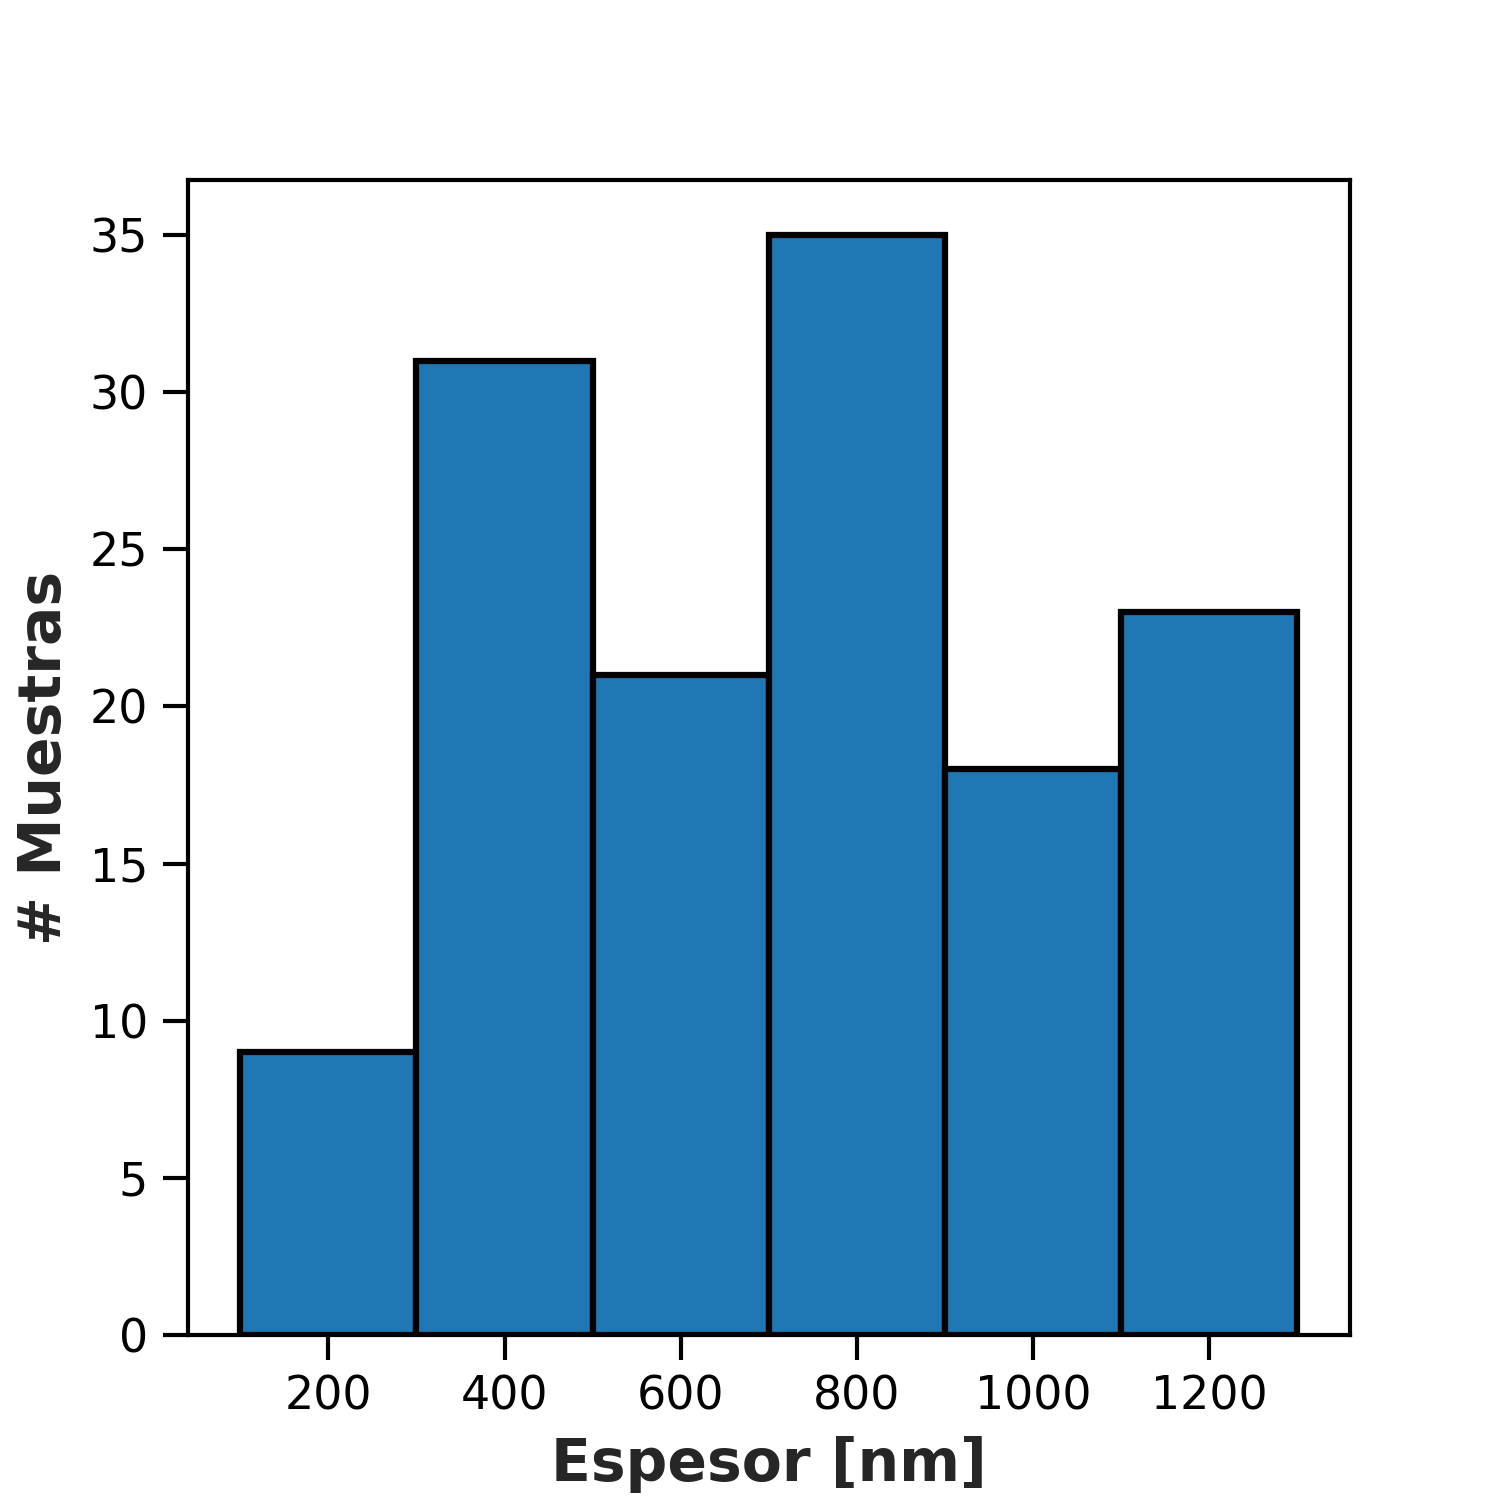
\includegraphics[width=0.7\textwidth]{bin_200.png}
\caption{Histograma de espesores con bins de 200 nm.}
\label{fig:bin200}
\end{figure}

\begin{figure}[htbp]
\centering
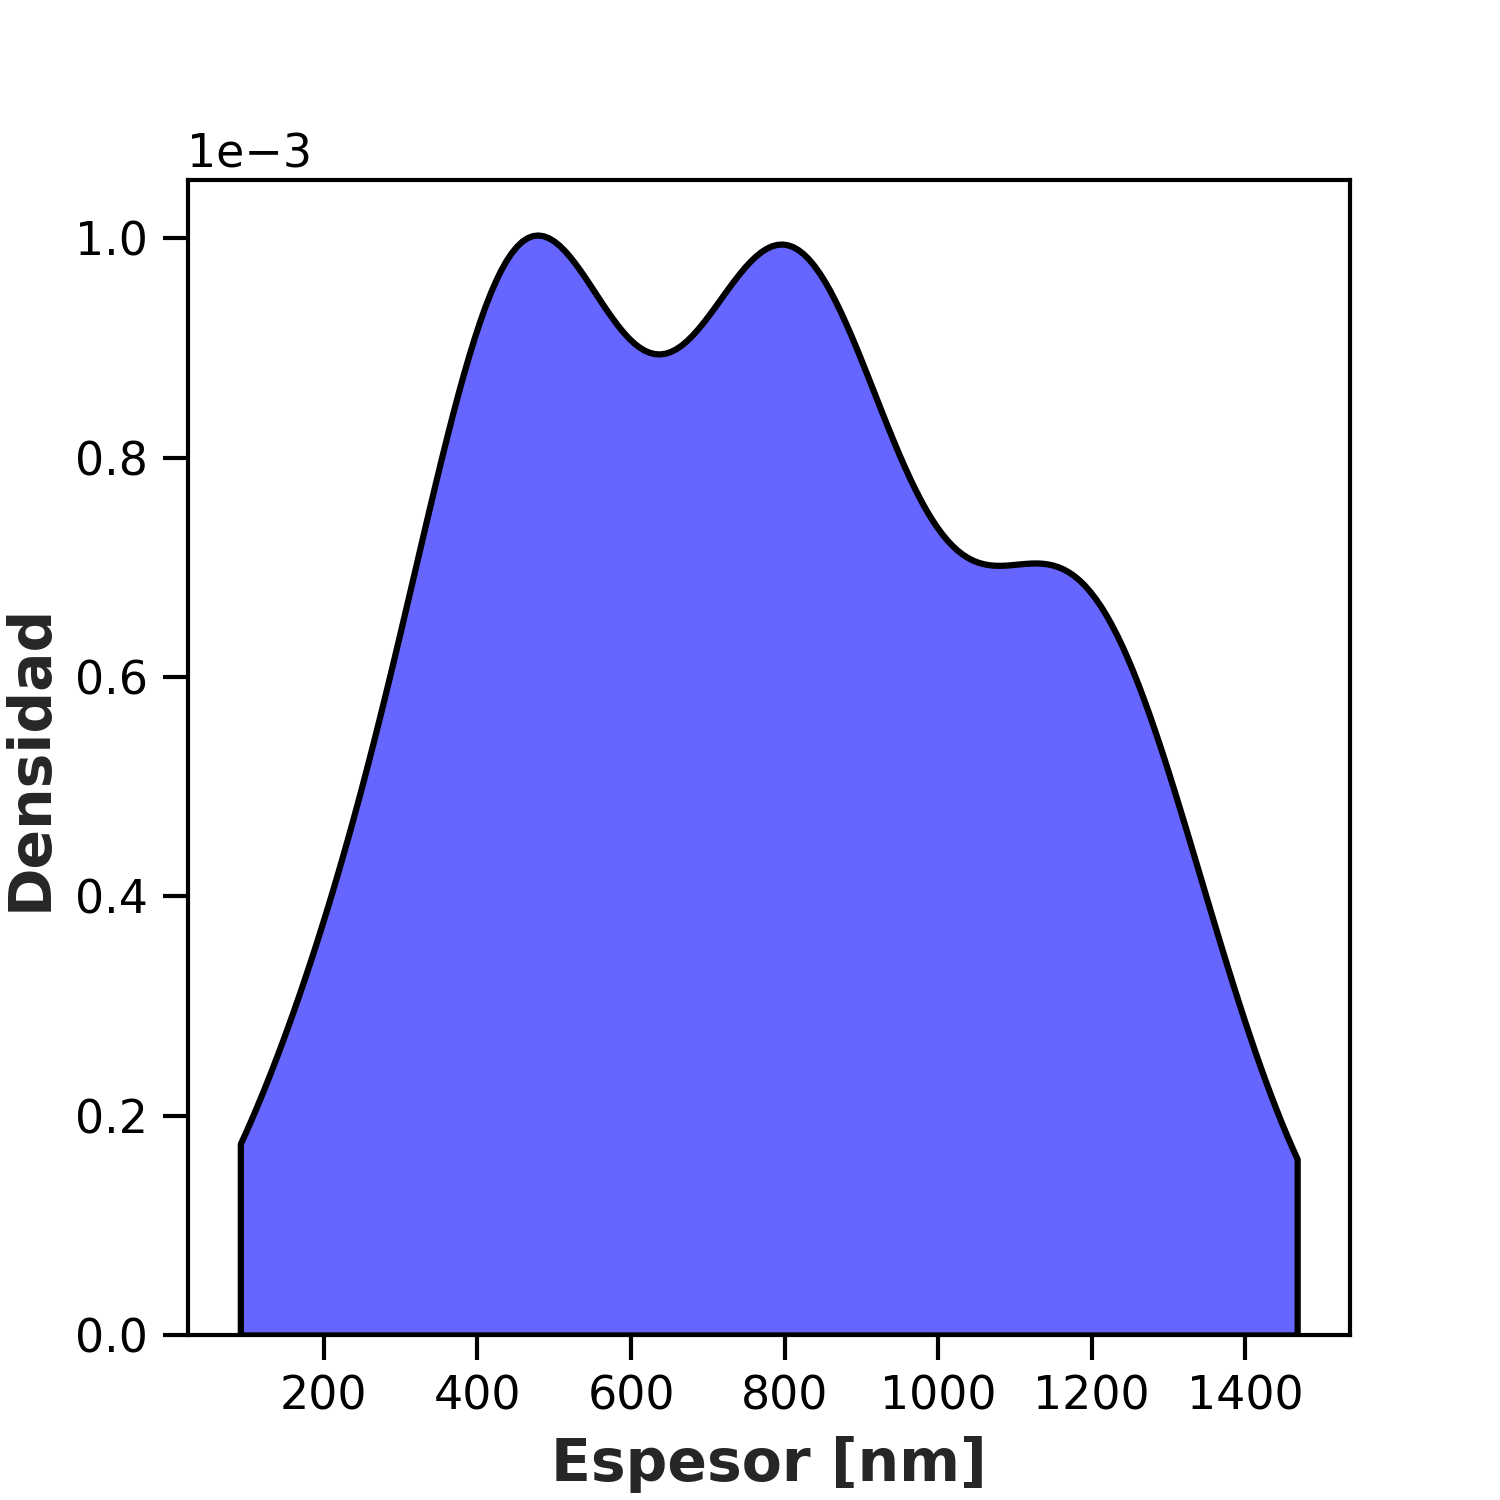
\includegraphics[width=0.7\textwidth]{kde.png}
\caption{Estimaci\'on de densidad KDE de la distribuci\'on de espesores.}
\label{fig:kde}
\end{figure}

\begin{figure}[htbp]
\centering
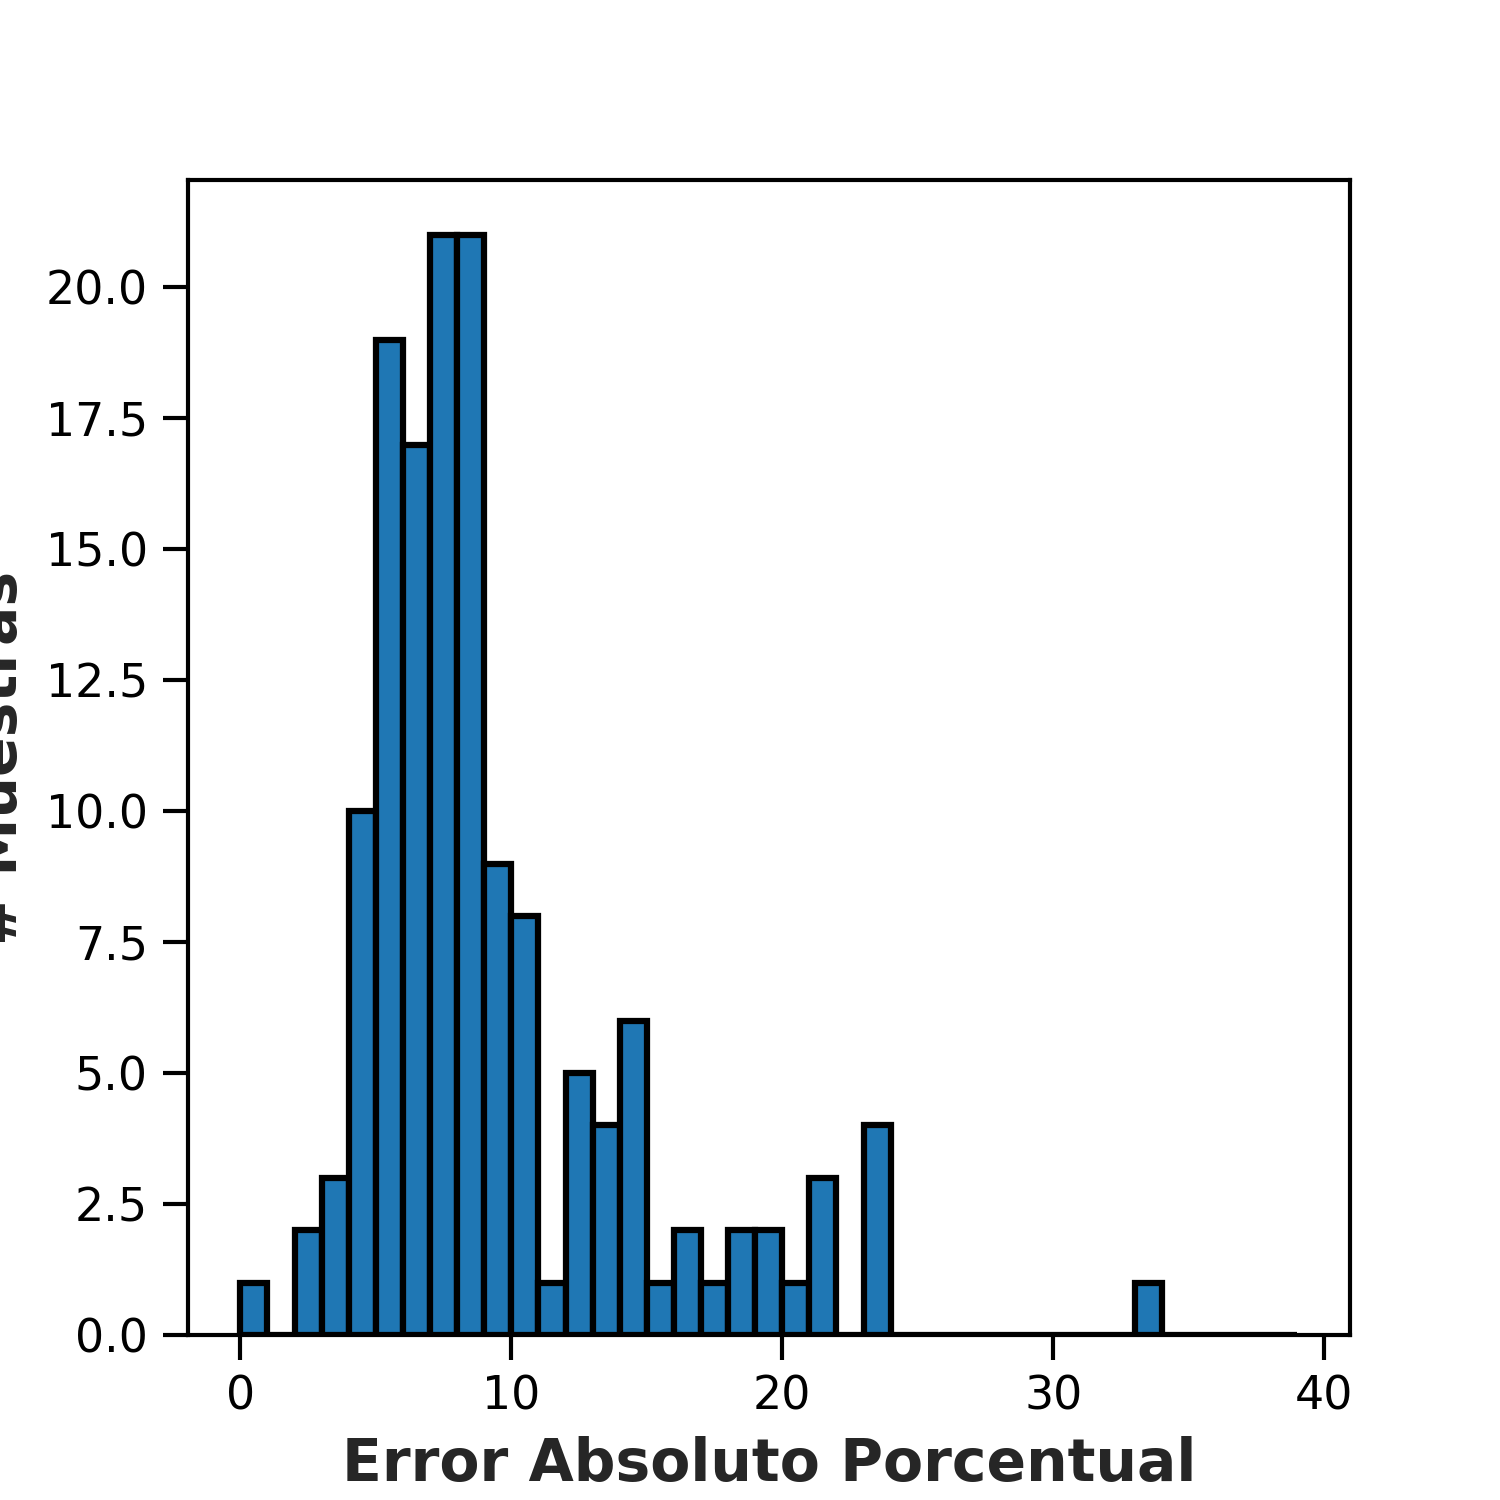
\includegraphics[width=0.7\textwidth]{error1.png}
\caption{Histograma de error porcentual de medici\'on de espesor.}
\label{fig:error1}
\end{figure}

% ============================================================
% CHAPTER 1: Estimación de Parámetros
% ============================================================
\section{Estimaci\'on de Par\'ametros: Ajuste del Modelo de Transmitancia}
\label{sec:param-est}

\subsection{Modelo de Transmitancia de Alonso}

El modelo f\'isico de transmitancia utilizado para describir el comportamiento \'optico de las pel\'iculas delgadas de AZO es el modelo de Alonso, que incorpora m\'ultiples componentes f\'isicas y un total de 13 par\'ametros:

\begin{itemize}
    \item \textbf{Par\'ametros geom\'etricos}: $x$ (longitud de onda, $\lambda$), $d$ (espesor de la pel\'icula)
    \item \textbf{Par\'ametros de rugosidad}: $R_1$ ($\sigma_1$), $R_2$ ($\sigma_2$)
    \item \textbf{Par\'ametros de Sellmeier}: $A, B, C, D, E$
    \item \textbf{Par\'ametros de absorci\'on}: $\alpha_0$ (amplitud de cola de Urbach), $\beta$ (energ\'ia de Urbach), $\lambda_g$ (\textit{band gap})
    \item \textbf{Portadores libres}: $n_e$ (densidad de electrones libres)
\end{itemize}

Los componentes f\'isicos del modelo incluyen:
\begin{enumerate}
    \item \textbf{Ecuaci\'on de Sellmeier}: describe la dependencia espectral del \'indice de refracci\'on $n(\lambda)$ en la regi\'on de transparencia.
    \item \textbf{Modelo de Drude}: modela la contribuci\'on de portadores libres (electrones) a las propiedades \'opticas.
    \item \textbf{Absorci\'on de cola de Urbach}: describe la absorci\'on exponencial cerca del borde de banda.
    \item \textbf{Correcciones de rugosidad}: mediante teor\'ia de dispersi\'on escalar (\textit{scalar scattering theory}) se modela el efecto de la rugosidad superficial en la transmitancia.
    \item \textbf{Transmitancia del sustrato de vidrio}: contribuci\'on independiente del sustrato.
\end{enumerate}

\textbf{Restricci\'on f\'isica}: $1.8 \leq n(\lambda) \leq 2.1$ para todo $\lambda$.

\textbf{Constantes}: $c = 3 \times 10^8$ m/s (velocidad de la luz), $\mu = 3.90 \times 10^{-4}$ m$^2$/Vs (movilidad de electrones).

\subsection{Algoritmos de Optimizaci\'on}

Se evaluaron tres algoritmos de optimizaci\'on para ajustar los 13 par\'ametros del modelo de Alonso a los espectros experimentales. En todos los casos, la funci\'on objetivo fue el Error Cuadr\'atico Medio (MSE) entre la transmitancia experimental y la simulada:

\subsubsection{Basin-Hopping (BH)}

Algoritmo de optimizaci\'on global estoc\'astica con optimizador local SLSQP y restricciones no lineales (\texttt{NonlinearConstraint}). Este m\'etodo explora el espacio de par\'ametros mediante saltos aleatorios (\textit{hopping}) seguidos de minimizaci\'on local.

\subsubsection{Evoluci\'on Diferencial (DE)}

Algoritmo evolutivo paralelo (\texttt{workers = -1}) con inicializaci\'on estoc\'astica mediante semillas (\textit{seeds}). Este m\'etodo explora el espacio de par\'ametros mediante una poblaci\'on de soluciones candidatas que evolucionan a trav\'es de mutaci\'on, cruza y selecci\'on.

\subsubsection{Direct}

M\'etodo de optimizaci\'on determinista con funci\'on de penalizaci\'on para manejar restricciones. Es el m\'as r\'apido pero el de menor calidad de ajuste.

\subsection{Resultados Comparativos}

El Cuadro~\ref{tab:optim-comp} presenta la comparaci\'on de los tres optimizadores.

\begin{table}[htbp]
\centering
\caption{Comparaci\'on de desempe\~no de los tres algoritmos de optimizaci\'on.}
\label{tab:optim-comp}
\begin{tabular}{@{}cccc@{}}
\toprule
\textbf{Optimizador} & \textbf{MSE Medio} & \textbf{Tiempo de Ejecuci\'on} & \textbf{Calidad} \\
\midrule
Evoluci\'on Diferencial (DE) & $\sim 0$ (mejor) & $\sim$ 4 horas & Excelente \\
Basin-Hopping (BH)           & $\sim 5$         & $\sim$ 12 horas & Moderada \\
Direct                       & $\sim 8$--30     & $\sim$ 5 minutos & Pobre \\
\bottomrule
\end{tabular}
\end{table}

Los tiempos de ejecuci\'on precisos por optimizador fueron:
\begin{itemize}
    \item Direct: 136.69 segundos ($\sim$ 2.3 minutos)
    \item DE: 4518.16 segundos ($\sim$ 1.25 horas)
    \item BH: 7995.91 segundos ($\sim$ 2.22 horas)
\end{itemize}

\begin{figure}[htbp]
\centering
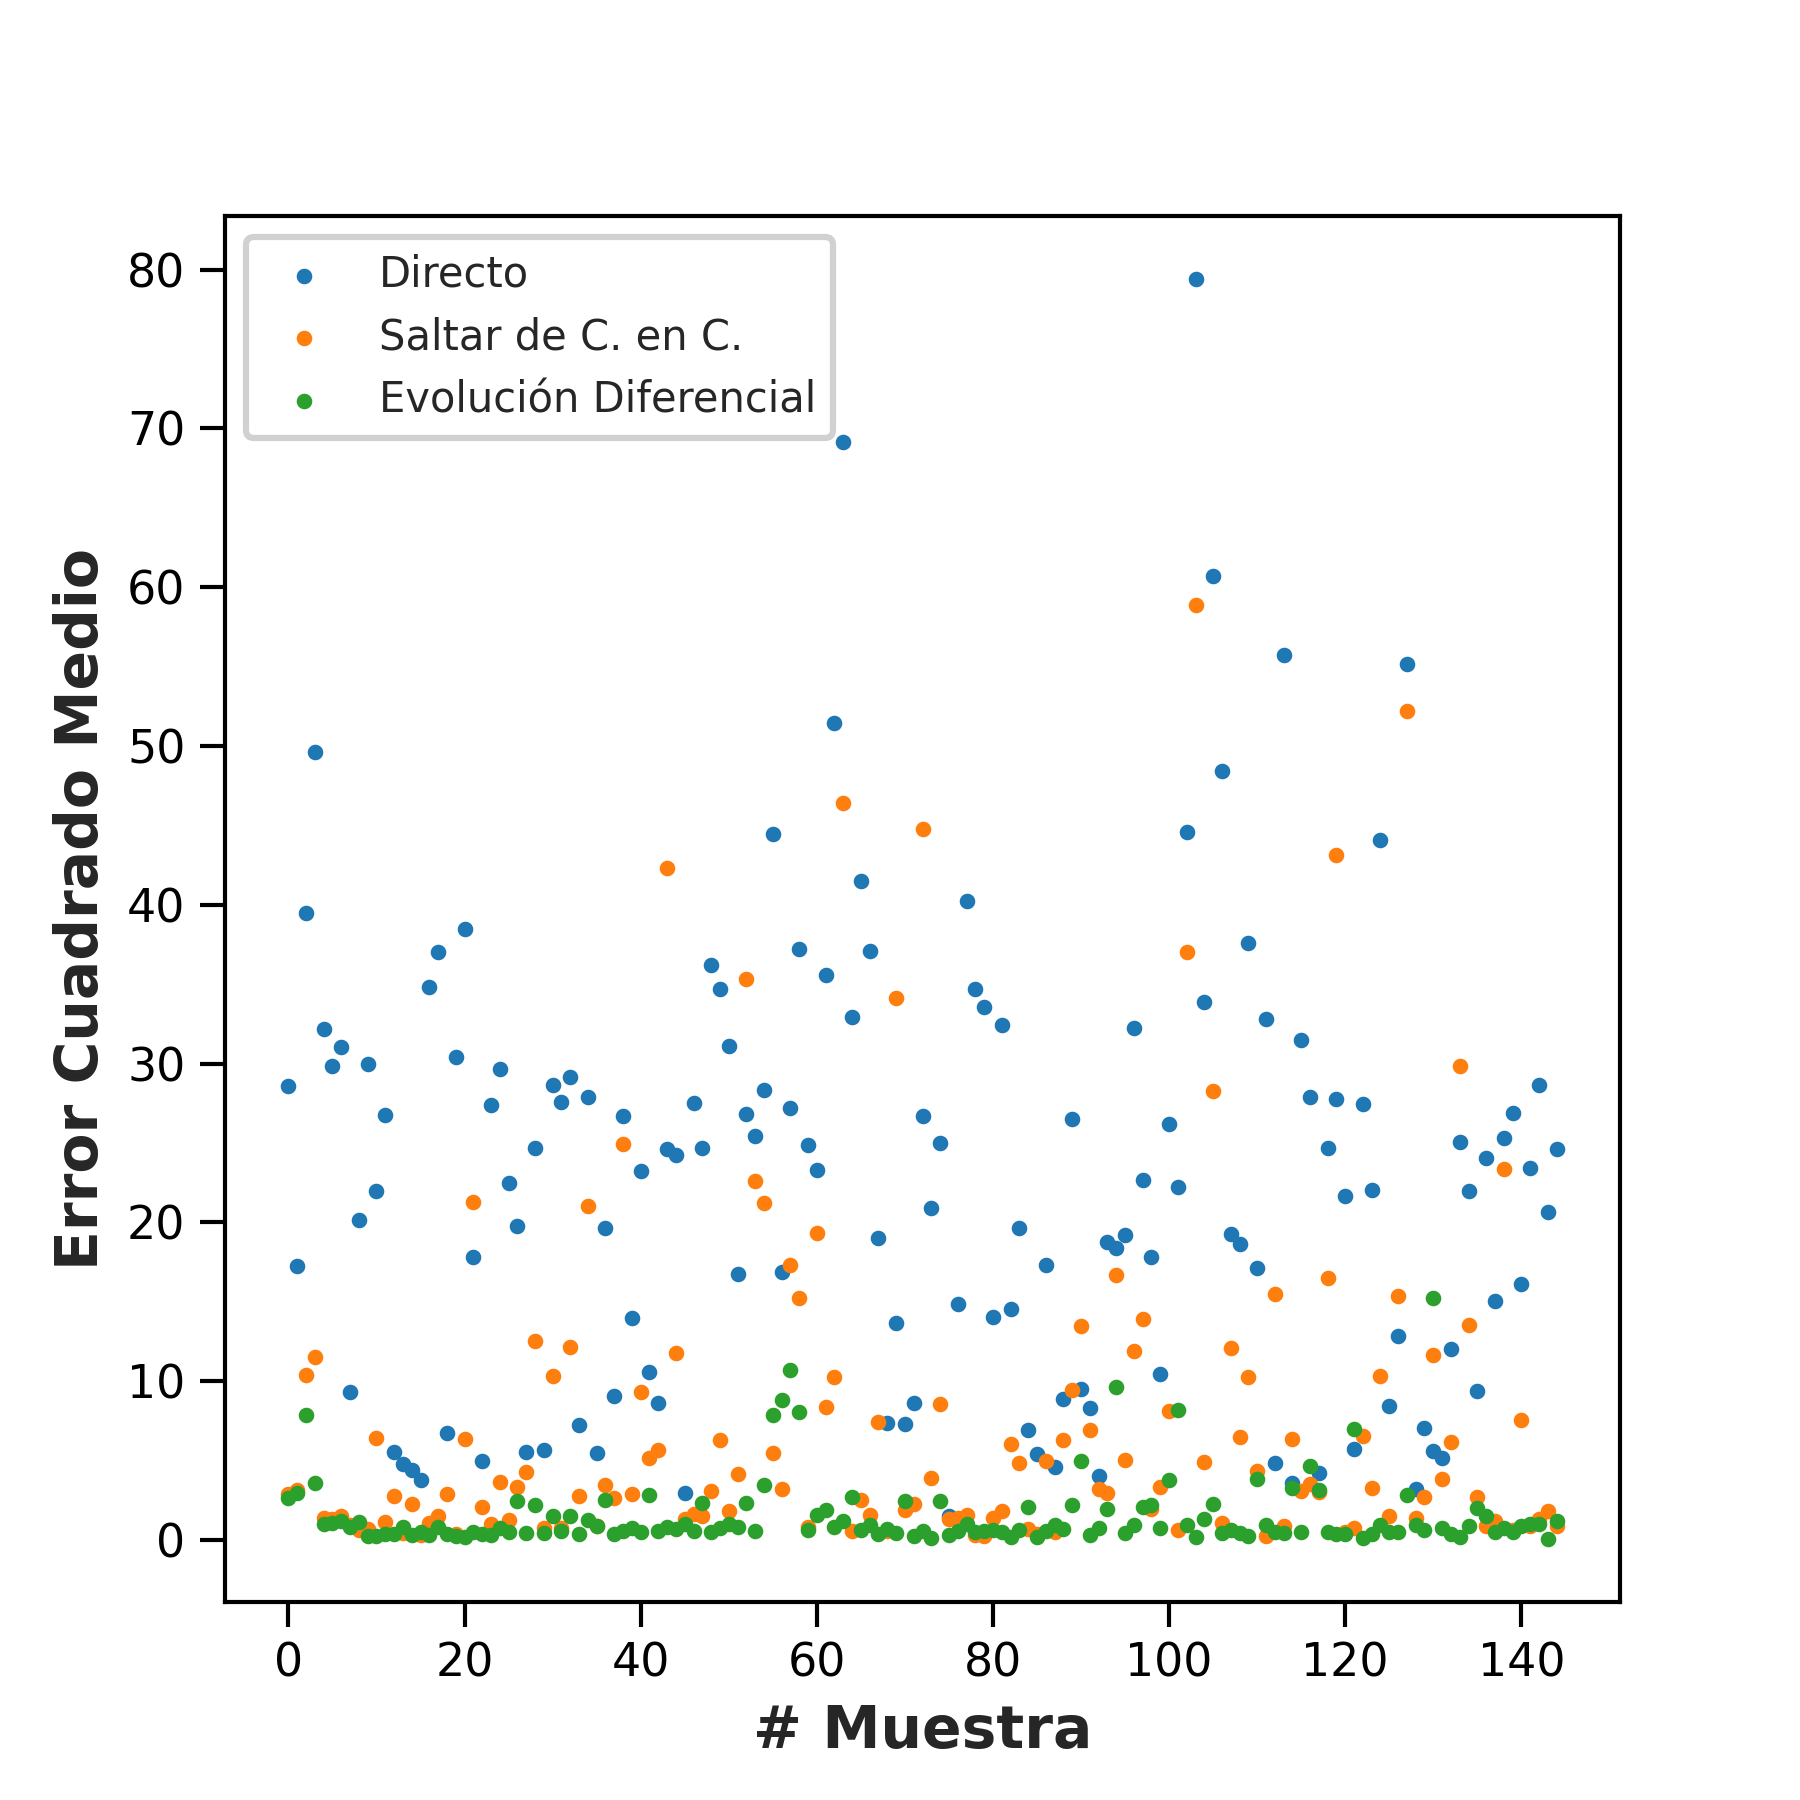
\includegraphics[width=0.9\textwidth]{comparative.png}
\caption{Gr\'afico de dispersi\'on del MSE por muestra para los tres algoritmos.}
\label{fig:comparative}
\end{figure}

\begin{figure}[htbp]
\centering
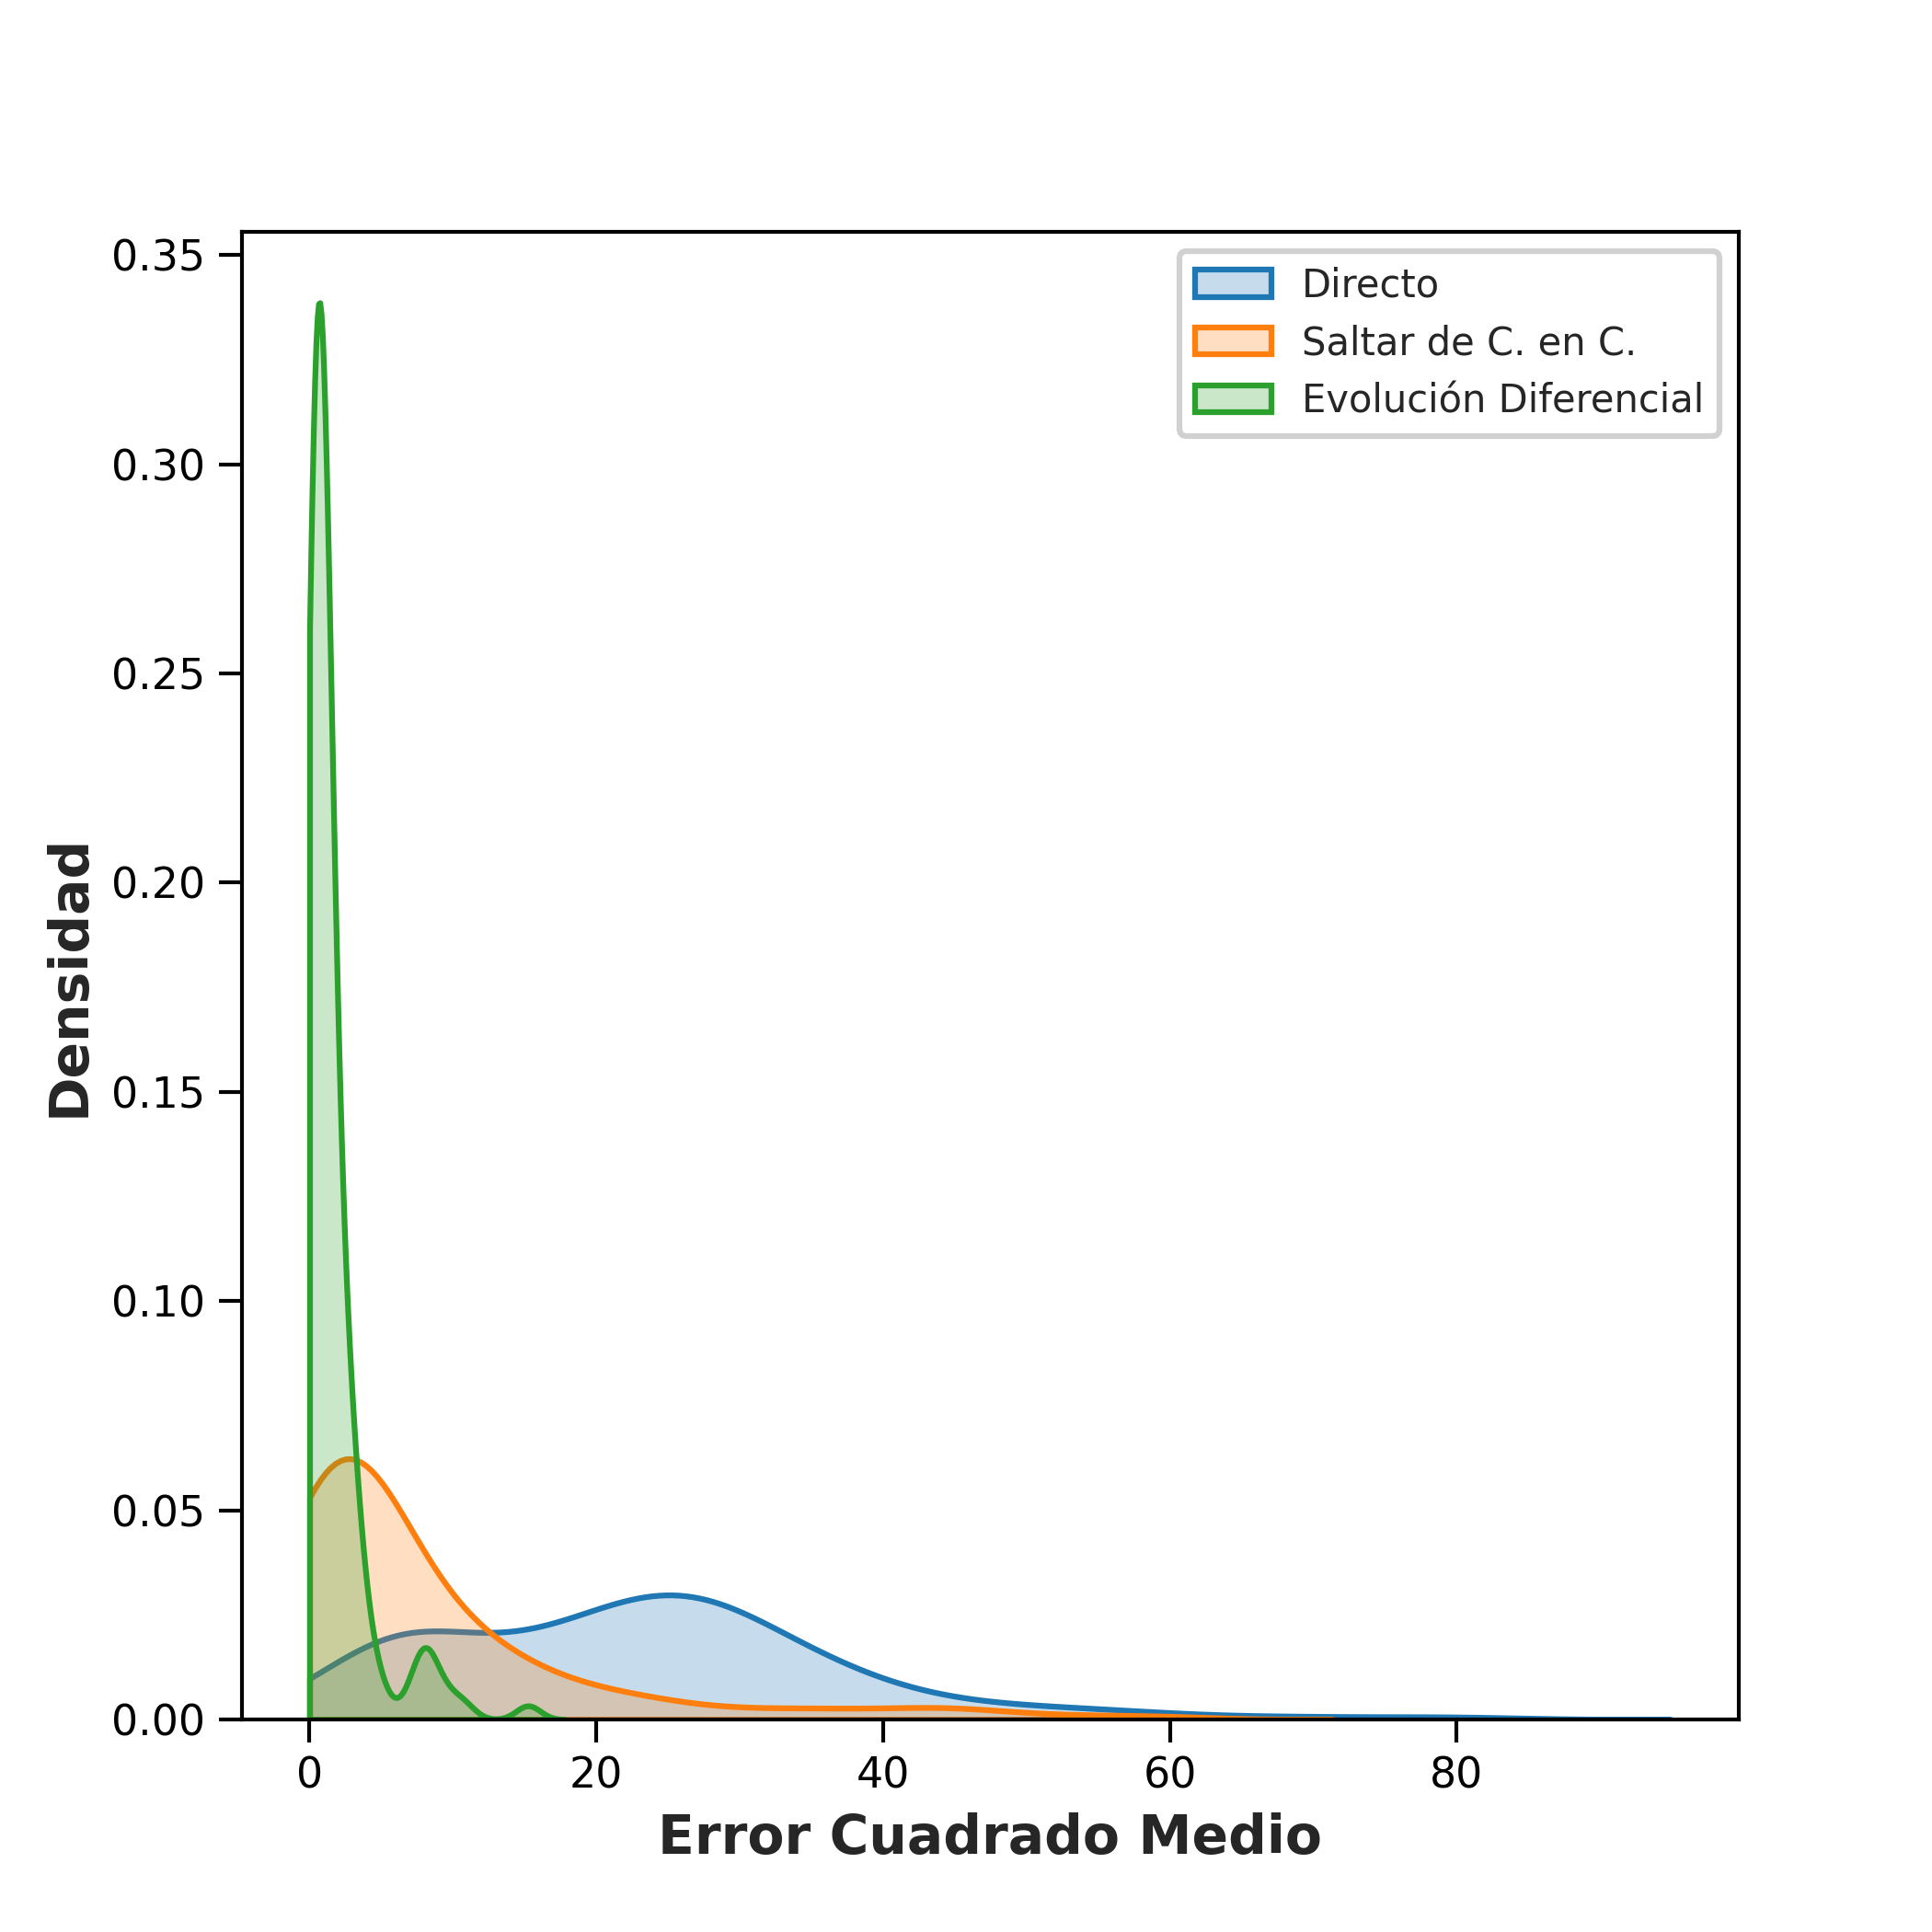
\includegraphics[width=0.8\textwidth]{kde_optimizers.png}
\caption{Estimaci\'on de densidad KDE de las distribuciones de MSE por optimizador.}
\label{fig:kde-opt}
\end{figure}

\begin{figure}[htbp]
\centering
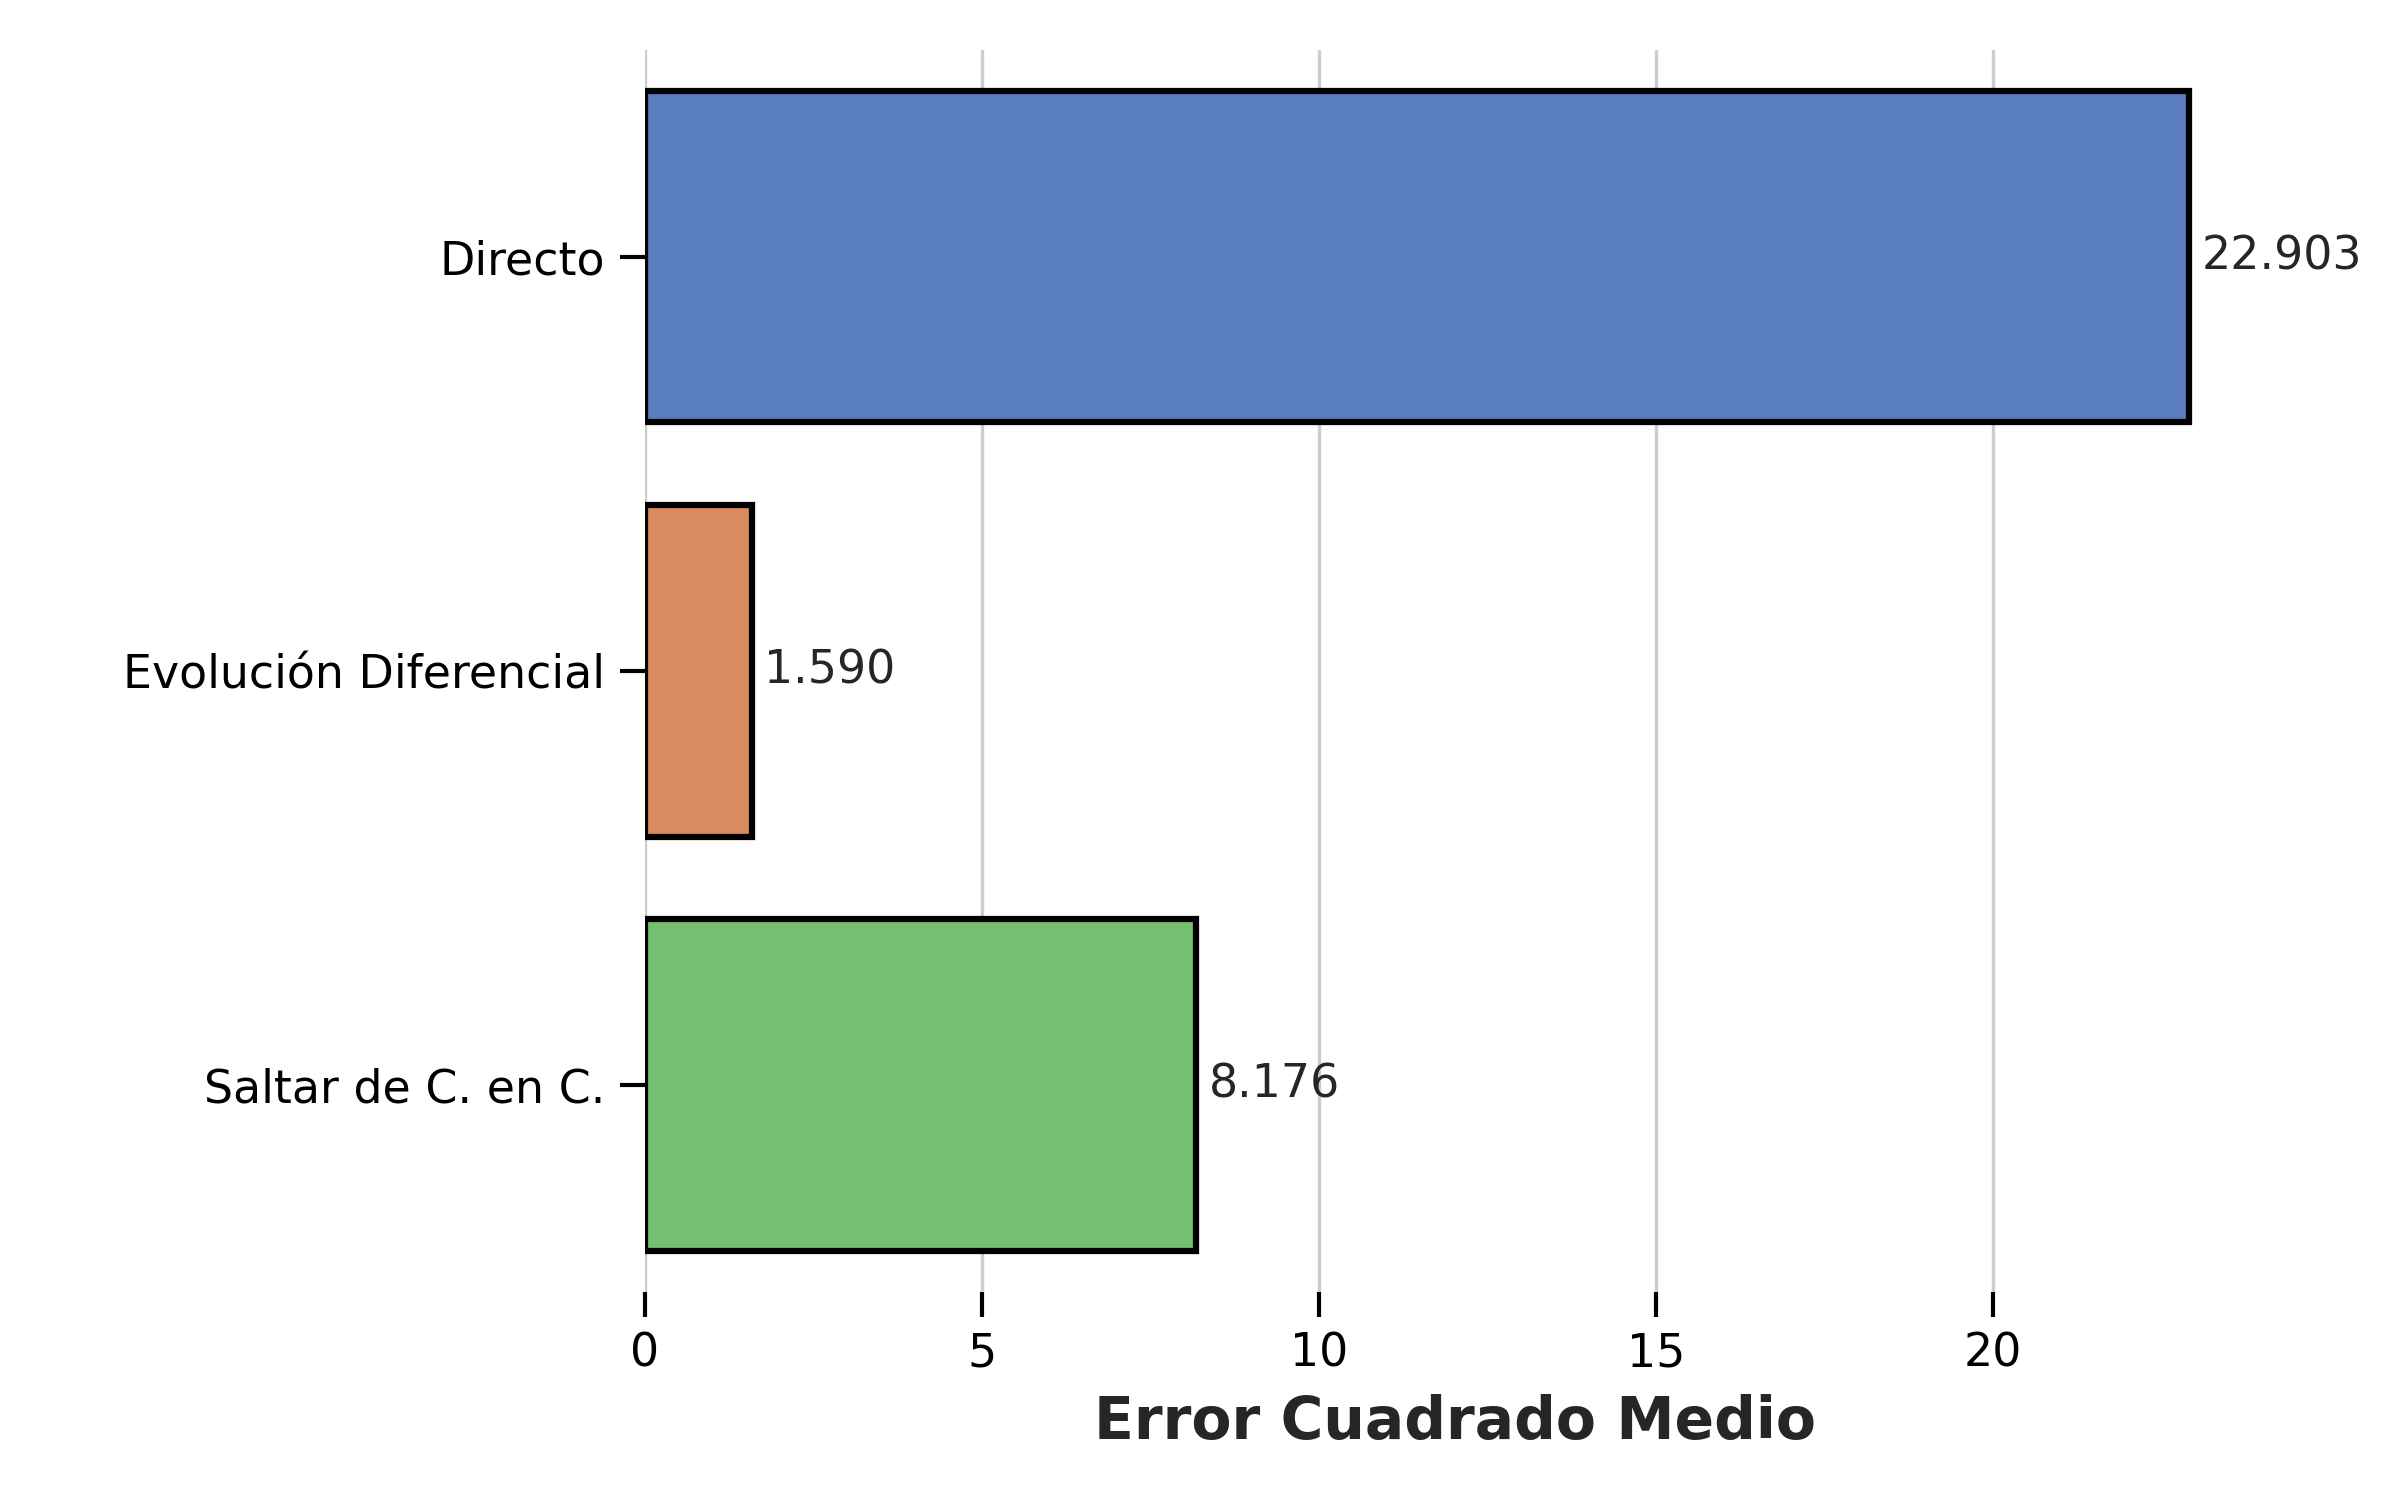
\includegraphics[width=0.7\textwidth]{final_comparative.png}
\caption{Comparaci\'on de barras del MSE medio por optimizador.}
\label{fig:final-comp}
\end{figure}

\subsection{An\'alisis de Sensibilidad: Rango de Longitud de Onda}

Se realiz\'o un an\'alisis de sensibilidad comparando el ajuste con el rango completo de longitudes de onda (190--1100 nm) versus un rango restringido (400--1100 nm). El Cuadro~\ref{tab:sens-mse} resume la comparaci\'on.

\begin{table}[htbp]
\centering
\caption{Comparaci\'on de MSE entre el rango completo (190--1100 nm) y el rango restringido (400--1100 nm).}
\label{tab:sens-mse}
\begin{tabular}{@{}ccc@{}}
\toprule
\textbf{Rango (nm)} & \textbf{MSE Medio} & \textbf{Observaci\'on} \\
\midrule
190--1100 & $\sim 0$ (con DE) & Ajuste \'optimo \\
400--1100 & Moderado & Reduce informaci\'on en UV \\
\bottomrule
\end{tabular}
\end{table}

\begin{figure}[htbp]
\centering
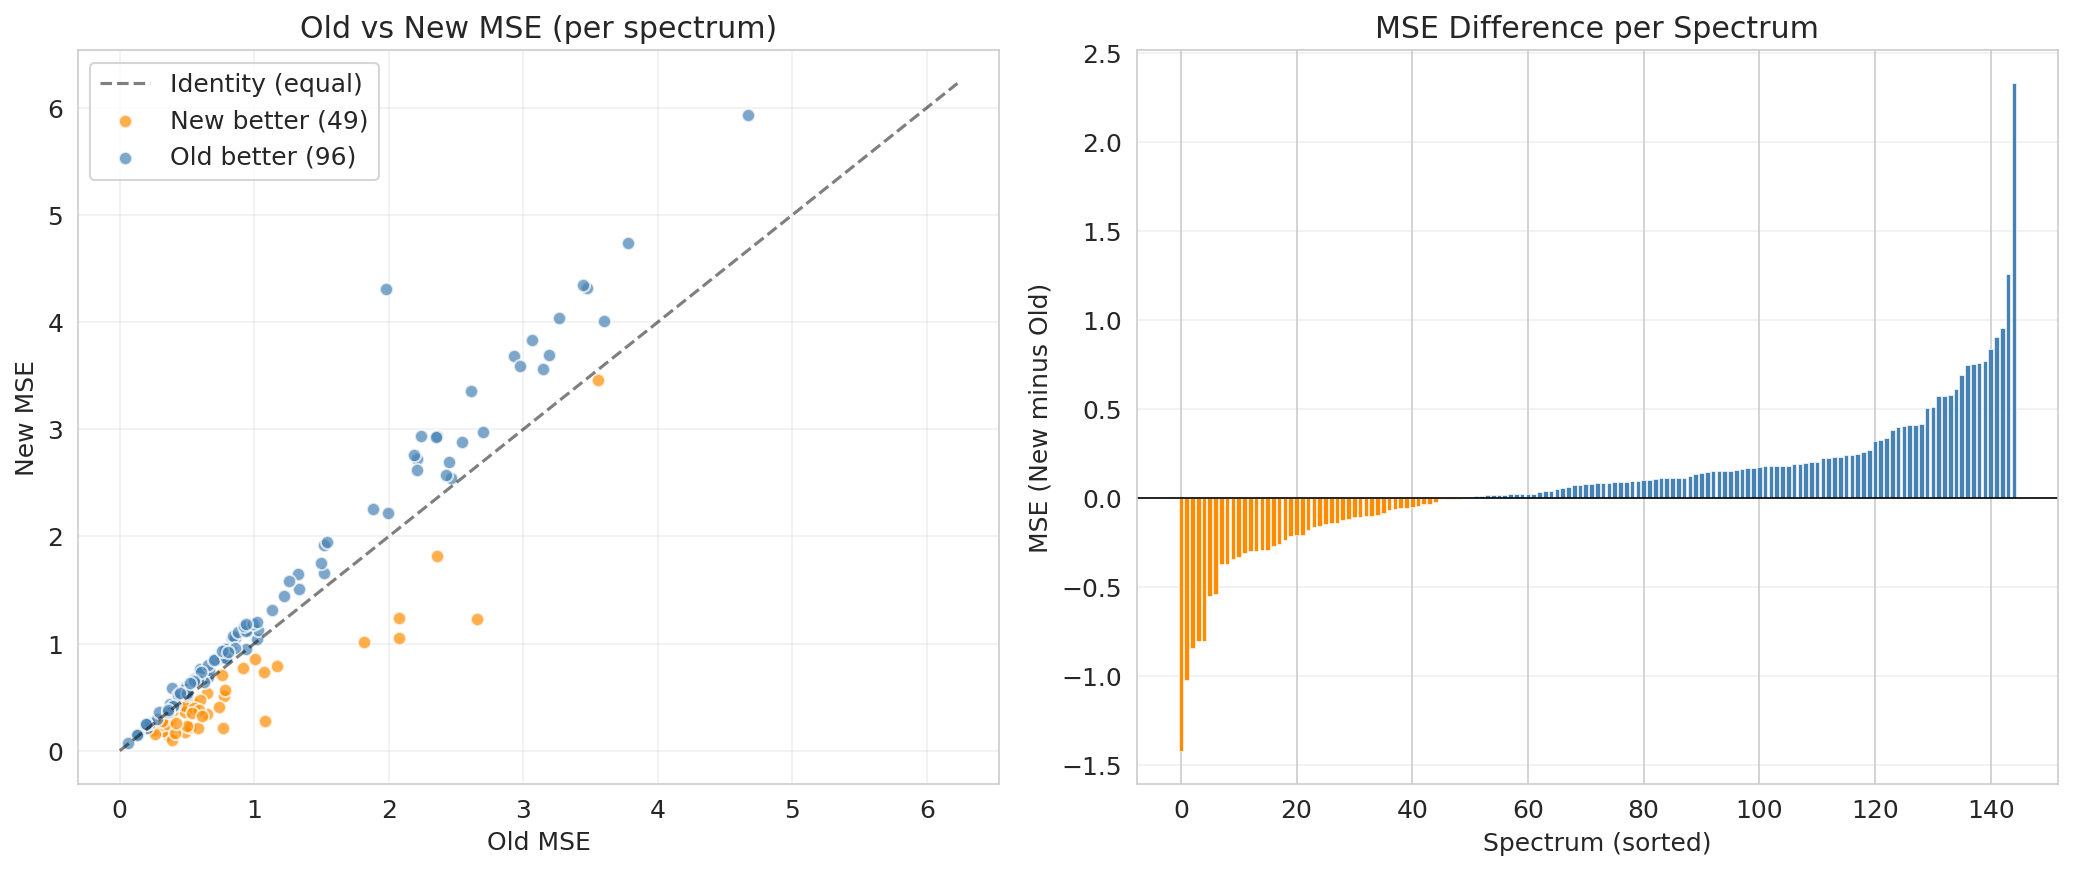
\includegraphics[width=0.8\textwidth]{mse_scatter_comparison.png}
\caption{Comparaci\'on de dispersi\'on MSE: rango completo vs 400--1100 nm.}
\label{fig:mse-scatter}
\end{figure}

\begin{figure}[htbp]
\centering
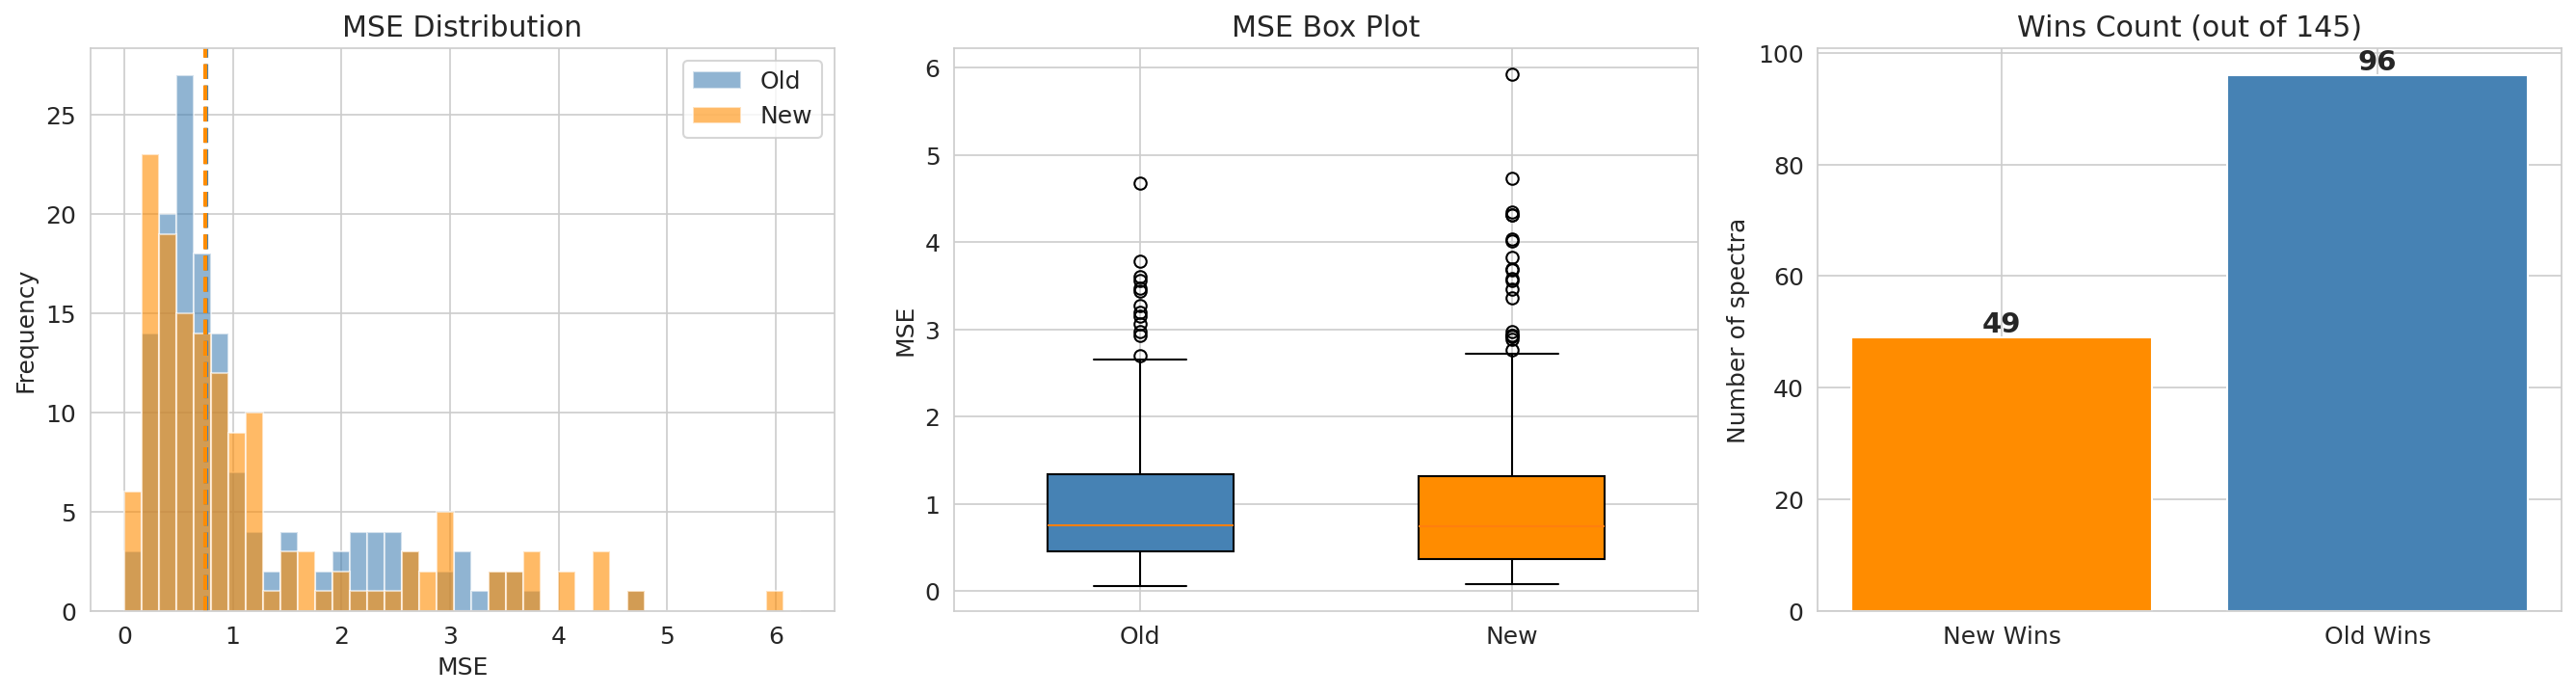
\includegraphics[width=0.7\textwidth]{mse_comparison_summary.png}
\caption{Resumen de comparaci\'on de m\'etricas MSE.}
\label{fig:mse-summary}
\end{figure}

\subsection{Conclusi\'on}

La Evoluci\'on Diferencial (DE) es el mejor optimizador para el ajuste del modelo de Alonso, proporcionando el MSE m\'as bajo ($\sim 0$) con un tiempo de ejecuci\'on aceptable ($\sim$ 1.25 horas). Se recomienda utilizar el rango completo de 190--1100 nm para la producci\'on, ya que proporciona informaci\'on espectral completa que mejora la calidad del ajuste.

% ============================================================
% CHAPTER 2: Análisis de Ajuste por Evolución Diferencial
% ============================================================
\section{An\'alisis de Ajuste por Evoluci\'on Diferencial}
\label{sec:de-analysis}

\subsection{Datos de Entrada y Flujo de An\'alisis}

Los datos de entrada para este an\'alisis consisten en:
\begin{itemize}
    \item Matriz \texttt{DE\_results} de dimensiones $(145, 14)$, conteniendo los 13 par\'ametros ajustados m\'as el MSE para cada muestra.
    \item \textit{DataFrame} experimental con los espectros de transmitancia y espesores medidos.
\end{itemize}

El flujo de an\'alisis comprende los siguientes pasos:
\begin{enumerate}
    \item Comparaci\'on de espectros: 145 gr\'aficas individuales de superposici\'on entre la transmitancia experimental y la simulada con par\'ametros DE.
    \item Cuadr\'iculas 3$\times$3: 17 cuadr\'iculas de resumen (16 completas + 1 con relleno) para inspecci\'on r\'apida.
    \item Distribuciones de MSE y espesores: histogramas y estimaciones de densidad KDE.
    \item An\'alisis estad\'istico por par\'ametro: funci\'on \texttt{analyze\_distribution} que calcula estad\'isticas b\'asicas, forma de distribuci\'on, pruebas de normalidad (Shapiro-Wilk, KS, Anderson-Darling, Jarque-Bera), comparaci\'on de cuantiles, detecci\'on de valores at\'ipicos, entrop\'ia, coeficiente de variaci\'on y figuras diagn\'osticas de 6 paneles.
    \item Ajuste GMM sobre el espesor mediante criterio BIC.
    \item An\'alisis por regiones: partici\'on en 5 intervalos de espesor.
    \item Gr\'aficos de cresta (\textit{ridge plots}) para visualizar distribuciones condicionadas por regi\'on.
\end{enumerate}

\subsection{Partici\'on por Regiones de Espesor}

El conjunto de 145 muestras se dividi\'o en 5 regiones basadas en el espesor $d$, como se muestra en el Cuadro~\ref{tab:regions}.

\begin{table}[htbp]
\centering
\caption{Partici\'on de las 145 muestras en 5 regiones de espesor.}
\label{tab:regions}
\begin{tabular}{@{}cccc@{}}
\toprule
\textbf{Regi\'on} & \textbf{Rango (nm)} & \textbf{Muestras} \\
\midrule
R$_1$ & $100$--$250$ & 8 \\
R$_2$ & $250$--$600$ & 47 \\
R$_3$ & $600$--$950$ & 46 \\
R$_4$ & $950$--$1100$ & 10 \\
R$_5$ & $1100$--$1500$ & 34 \\
\bottomrule
\end{tabular}
\end{table}

\subsection{Estad\'isticas de Par\'ametros: Espesor ($d$) y Sellmeier $A$}

A continuaci\'on se presentan las estad\'isticas descriptivas completas para el par\'ametro de espesor ($d$) y el par\'ametro Sellmeier $A$, obtenidas mediante la funci\'on \texttt{analyze\_distribution}.

\subsubsection{Par\'ametro: Espesor ($d$, nm)}

\begin{table}[htbp]
\centering
\caption{Estad\'isticas descriptivas del par\'ametro de espesor $d$ (nm) -- 145 muestras.}
\label{tab:stats-d}
\begin{tabular}{@{}lc@{}}
\toprule
\textbf{Estad\'istica} & \textbf{Valor} \\
\midrule
Tama\~no de muestra ($n$) & 145 \\
Media ($\bar{x}$) & 772.3146 \\
Mediana & 783.2036 \\
Desviaci\'on est\'andar ($\sigma$) & 339.2029 \\
Varianza ($\sigma^2$) & 115058.6111 \\
M\'inimo & 103.5237 \\
M\'aximo & 1476.0822 \\
Rango & 1372.5586 \\
IQR & 577.9567 \\
\midrule
Asimetr\'ia & 0.1570 \\
Curtosis (exceso) & $-0.9997$ \\
Coeficiente de variaci\'on & 0.4392 \\
Entrop\'ia & 2.9509 bits \\
\midrule
\textit{Outliers} (IQR) & 0 (0.00\%) \\
\midrule
\multicolumn{2}{c}{\textbf{Pruebas de Normalidad}} \\
\midrule
Shapiro-Wilk & $W = 0.9637$, $p = 0.000706$ \\
Kolmogorov-Smirnov & $D = 0.1209$, $p = 0.026356$ \\
Anderson-Darling & $A^2 = 1.7532$ (cr\'itico 5\%: 0.7670) \\
Jarque-Bera & $JB = 6.7051$, $p = 0.034995$ \\
\bottomrule
\end{tabular}
\end{table}

\begin{table}[htbp]
\centering
\caption{Comparaci\'on de cuantiles para espesor $d$: emp\'irico vs normal te\'orico.}
\label{tab:quant-d}
\begin{tabular}{@{}cccc@{}}
\toprule
\textbf{Cuantil} & \textbf{Emp\'irico} & \textbf{Normal} & \textbf{Diferencia} \\
\midrule
0.01 & 178.5707 & $-16.7894$ & 195.3600 \\
0.05 & 241.9872 & 214.3755 & 27.6118 \\
0.25 & 475.9550 & 543.5257 & $-67.5708$ \\
0.50 & 783.2036 & 772.3146 & 10.8890 \\
0.75 & 1053.9117 & 1001.1035 & 52.8082 \\
0.95 & 1286.8495 & 1330.2537 & $-43.4042$ \\
0.99 & 1436.9976 & 1561.4186 & $-124.4210$ \\
\bottomrule
\end{tabular}
\end{table}

\subsubsection{Par\'ametro: Sellmeier $A$}

\begin{table}[htbp]
\centering
\caption{Estad\'isticas descriptivas del par\'ametro Sellmeier $A$ -- 145 muestras.}
\label{tab:stats-A}
\begin{tabular}{@{}lc@{}}
\toprule
\textbf{Estad\'istica} & \textbf{Valor} \\
\midrule
Tama\~no de muestra ($n$) & 145 \\
Media ($\bar{x}$) & 3.4135 \\
Mediana & 3.2490 \\
Desviaci\'on est\'andar ($\sigma$) & 0.3186 \\
Varianza ($\sigma^2$) & 0.1015 \\
M\'inimo & 3.2400 \\
M\'aximo & 4.4097 \\
Rango & 1.1697 \\
IQR & 0.1526 \\
\midrule
Asimetr\'ia & 1.9490 \\
Curtosis (exceso) & 2.6042 \\
Coeficiente de variaci\'on & 0.0933 \\
Entrop\'ia & 2.1519 bits \\
\midrule
\textit{Outliers} (IQR) & 24 (16.55\%) \\
\midrule
\multicolumn{2}{c}{\textbf{Pruebas de Normalidad}} \\
\midrule
Shapiro-Wilk & $W = 0.6058$, $p < 0.000001$ \\
Kolmogorov-Smirnov & $D = 0.3277$, $p < 0.000001$ \\
Anderson-Darling & $A^2 = 24.8658$ (cr\'itico 5\%: 0.7670) \\
Jarque-Bera & $JB = 126.8835$, $p < 0.000001$ \\
\bottomrule
\end{tabular}
\end{table}

\subsection{An\'alisis por Regiones: Region R$_1$ (Bin 0, $100$--$250$ nm, 8 muestras)}

El Cuadro~\ref{tab:bin0} presenta las estad\'isticas de los 13 par\'ametros para la Regi\'on R$_1$.

\begin{table}[htbp]
\centering
\caption{Estad\'isticas por par\'ametro para la Regi\'on R$_1$ ($100$--$250$ nm, 8 muestras).}
\label{tab:bin0}
\begin{tabular}{@{}lcccccccc@{}} % Modified: removed one column to align properly
\toprule
\textbf{Par\'ametro} & \textbf{M\'in} & \textbf{M\'ax} & $\boldsymbol{\bar{x}}$ & $\boldsymbol{\delta(x)}$ & \textbf{Mediana} & \textbf{IQR} & \textbf{Asim.} & \textbf{Curt.} \\
\midrule
$r$ [nm] & $1.035 \times 10^2$ & $2.389 \times 10^2$ & $2.021 \times 10^2$ & $4.388 \times 10^1$ & $2.229 \times 10^2$ & $4.932 \times 10^1$ & $-1.245$ & $3.802 \times 10^{-1}$ \\
$\sigma_{1}$ [nm] & $5.000$ & $3.996 \times 10^1$ & $1.844 \times 10^1$ & $1.068 \times 10^1$ & $1.436 \times 10^1$ & $1.328 \times 10^1$ & $7.778 \times 10^{-1}$ & $-4.624 \times 10^{-1}$ \\
$\sigma_{2}$ [nm] & $5.000$ & $3.754 \times 10^1$ & $1.281 \times 10^1$ & $9.994$ & $7.863$ & $7.395$ & $1.759$ & $1.773$ \\
$A$ & $3.240$ & $4.410$ & $3.607$ & $4.459 \times 10^{-1}$ & $3.315$ & $7.890 \times 10^{-1}$ & $6.900 \times 10^{-1}$ & $-1.245$ \\
$B$ & $1.684 \times 10^5$ & $1.970 \times 10^6$ & $6.568 \times 10^5$ & $6.021 \times 10^5$ & $3.764 \times 10^5$ & $4.948 \times 10^5$ & $1.282$ & $1.259 \times 10^{-1}$ \\
$C$ [nm] & $1.927 \times 10^6$ & $1.444 \times 10^7$ & $9.539 \times 10^6$ & $3.474 \times 10^6$ & $9.538 \times 10^6$ & $2.870 \times 10^6$ & $-8.922 \times 10^{-1}$ & $4.464 \times 10^{-1}$ \\
$D$ & $5.000 \times 10^{-1}$ & $2.998$ & $8.927 \times 10^{-1}$ & $7.990 \times 10^{-1}$ & $6.357 \times 10^{-1}$ & $1.634 \times 10^{-1}$ & $2.231$ & $3.050$ \\
$E$ [nm] & $1.350 \times 10^2$ & $3.419 \times 10^2$ & $2.589 \times 10^2$ & $8.315 \times 10^1$ & $2.830 \times 10^2$ & $1.309 \times 10^2$ & $-4.529 \times 10^{-1}$ & $-1.410$ \\
$\alpha_{0}$ [nm$^{-1}$] & $1.106 \times 10^{-3}$ & $1.333 \times 10^{-2}$ & $5.866 \times 10^{-3}$ & $3.885 \times 10^{-3}$ & $5.427 \times 10^{-3}$ & $4.522 \times 10^{-3}$ & $5.662 \times 10^{-1}$ & $-6.593 \times 10^{-1}$ \\
$\beta$ [eV$^{-1}$] & $4.793$ & $1.273 \times 10^1$ & $9.774$ & $2.787$ & $1.052 \times 10^1$ & $2.987$ & $-8.363 \times 10^{-1}$ & $-8.402 \times 10^{-1}$ \\
$\lambda_{g}$ [nm] & $3.542 \times 10^2$ & $3.824 \times 10^2$ & $3.678 \times 10^2$ & $8.947$ & $3.694 \times 10^2$ & $1.282 \times 10^1$ & $2.041 \times 10^{-3}$ & $-1.116$ \\
$n_{e}$ [nm$^{-3}$] & $5.004 \times 10^{25}$ & $7.500 \times 10^{26}$ & $1.383 \times 10^{26}$ & $2.312 \times 10^{26}$ & $5.052 \times 10^{25}$ & $1.709 \times 10^{24}$ & $2.268$ & $3.142$ \\
$n(\lambda)$ & $1.166$ & $9.622$ & $5.375$ & $3.096$ & $5.389$ & $5.266$ & $6.788 \times 10^{-3}$ & $-1.746$ \\
\bottomrule
\end{tabular}
\end{table}

\subsection{An\'alisis por Regiones: Regi\'on R$_3$ (Bin 2, $600$--$950$ nm, 46 muestras)}

El Cuadro~\ref{tab:bin2} presenta las estad\'isticas para la Regi\'on R$_3$.

\begin{table}[htbp]
\centering
\caption{Estad\'isticas por par\'ametro para la Regi\'on R$_3$ ($600$--$950$ nm, 46 muestras).}
\label{tab:bin2}
\begin{tabular}{@{}lcccccccc@{}} % Modified: removed one column
\toprule
\textbf{Par\'ametro} & \textbf{M\'in} & \textbf{M\'ax} & $\boldsymbol{\bar{x}}$ & $\boldsymbol{\delta(x)}$ & \textbf{Mediana} & \textbf{IQR} & \textbf{Asim.} & \textbf{Curt.} \\
\midrule
$r$ [nm] & $6.174 \times 10^2$ & $9.424 \times 10^2$ & $7.974 \times 10^2$ & $7.527 \times 10^1$ & $8.149 \times 10^2$ & $1.031 \times 10^2$ & $-4.894 \times 10^{-1}$ & $-1.871 \times 10^{-1}$ \\
$\sigma_{1}$ [nm] & $5.000$ & $6.304 \times 10^1$ & $2.229 \times 10^1$ & $1.405 \times 10^1$ & $1.850 \times 10^1$ & $1.866 \times 10^1$ & $9.480 \times 10^{-1}$ & $2.092 \times 10^{-1}$ \\
$\sigma_{2}$ [nm] & $5.000$ & $7.374 \times 10^1$ & $2.355 \times 10^1$ & $1.481 \times 10^1$ & $2.297 \times 10^1$ & $1.831 \times 10^1$ & $1.032$ & $1.200$ \\
$A$ & $3.240$ & $4.385$ & $3.390$ & $3.029 \times 10^{-1}$ & $3.246$ & $1.009 \times 10^{-1}$ & $2.155$ & $3.336$ \\
$B$ & $1.199 \times 10^5$ & $2.317 \times 10^6$ & $1.381 \times 10^6$ & $5.408 \times 10^5$ & $1.343 \times 10^6$ & $7.029 \times 10^5$ & $-3.148 \times 10^{-1}$ & $-3.332 \times 10^{-1}$ \\
$C$ [nm] & $7.366 \times 10^5$ & $1.381 \times 10^7$ & $3.259 \times 10^6$ & $3.090 \times 10^6$ & $2.288 \times 10^6$ & $1.486 \times 10^6$ & $2.212$ & $4.021$ \\
$D$ & $5.000 \times 10^{-1}$ & $3.165$ & $7.197 \times 10^{-1}$ & $4.485 \times 10^{-1}$ & $5.154 \times 10^{-1}$ & $2.113 \times 10^{-1}$ & $3.767$ & $1.670 \times 10^1$ \\
$E$ [nm] & $1.401 \times 10^2$ & $3.517 \times 10^2$ & $3.101 \times 10^2$ & $3.877 \times 10^1$ & $3.193 \times 10^2$ & $2.204 \times 10^1$ & $-2.929$ & $9.414$ \\
$\alpha_{0}$ [nm$^{-1}$] & $8.113 \times 10^{-4}$ & $1.340 \times 10^{-2}$ & $6.201 \times 10^{-3}$ & $3.737 \times 10^{-3}$ & $5.172 \times 10^{-3}$ & $6.470 \times 10^{-3}$ & $3.476 \times 10^{-1}$ & $-1.186$ \\
$\beta$ [eV$^{-1}$] & $7.086$ & $1.297 \times 10^1$ & $1.023 \times 10^1$ & $1.241$ & $9.823$ & $1.800$ & $4.089 \times 10^{-1}$ & $-1.411 \times 10^{-1}$ \\
$\lambda_{g}$ [nm] & $3.469 \times 10^2$ & $3.822 \times 10^2$ & $3.605 \times 10^2$ & $8.488$ & $3.598 \times 10^2$ & $1.313 \times 10^1$ & $4.272 \times 10^{-1}$ & $-5.691 \times 10^{-1}$ \\
$n_{e}$ [nm$^{-3}$] & $5.003 \times 10^{25}$ & $6.019 \times 10^{26}$ & $1.509 \times 10^{26}$ & $1.092 \times 10^{26}$ & $1.246 \times 10^{26}$ & $1.227 \times 10^{26}$ & $1.891$ & $4.522$ \\
$n(\lambda)$ & $6.120 \times 10^{-2}$ & $4.975$ & $1.121$ & $1.098$ & $7.813 \times 10^{-1}$ & $5.861 \times 10^{-1}$ & $1.988$ & $3.582$ \\
\bottomrule
\end{tabular}
\end{table}

% Additional region tables for completeness
\subsection{An\'alisis por Regiones: Regi\'on R$_2$ (Bin 1, $250$--$600$ nm, 47 muestras)}

\begin{table}[htbp]
\centering
\caption{Estad\'isticas por par\'ametro para la Regi\'on R$_2$ ($250$--$600$ nm, 47 muestras).}
\label{tab:bin1}
\begin{tabular}{@{}lcccccccc@{}} % Modified: removed one column
\toprule
\textbf{Par\'ametro} & \textbf{M\'in} & \textbf{M\'ax} & $\boldsymbol{\bar{x}}$ & $\boldsymbol{\delta(x)}$ & \textbf{Mediana} & \textbf{IQR} & \textbf{Asim.} & \textbf{Curt.} \\
\midrule
$r$ [nm] & $2.541 \times 10^2$ & $5.870 \times 10^2$ & $4.502 \times 10^2$ & $7.467 \times 10^1$ & $4.641 \times 10^2$ & $1.080 \times 10^2$ & $-6.521 \times 10^{-1}$ & $1.204 \times 10^{-1}$ \\
$\sigma_{1}$ [nm] & $5.000$ & $6.283 \times 10^1$ & $1.913 \times 10^1$ & $1.323 \times 10^1$ & $1.663 \times 10^1$ & $1.709 \times 10^1$ & $1.188$ & $1.133$ \\
$\sigma_{2}$ [nm] & $5.000$ & $6.757 \times 10^1$ & $2.368 \times 10^1$ & $1.658 \times 10^1$ & $1.963 \times 10^1$ & $2.536 \times 10^1$ & $7.391 \times 10^{-1}$ & $-4.584 \times 10^{-1}$ \\
$A$ & $3.240$ & $4.404$ & $3.527$ & $3.740 \times 10^{-1}$ & $3.294$ & $4.066 \times 10^{-1}$ & $1.141$ & $-6.842 \times 10^{-2}$ \\
$B$ & $6.430 \times 10^4$ & $2.202 \times 10^6$ & $9.982 \times 10^5$ & $7.285 \times 10^5$ & $1.050 \times 10^6$ & $1.348 \times 10^6$ & $2.924 \times 10^{-2}$ & $-1.520$ \\
$C$ [nm] & $6.086 \times 10^5$ & $1.466 \times 10^7$ & $6.776 \times 10^6$ & $4.721 \times 10^6$ & $5.348 \times 10^6$ & $9.311 \times 10^6$ & $1.981 \times 10^{-1}$ & $-1.530$ \\
$D$ & $5.000 \times 10^{-1}$ & $2.351$ & $8.541 \times 10^{-1}$ & $5.582 \times 10^{-1}$ & $5.094 \times 10^{-1}$ & $4.452 \times 10^{-1}$ & $1.512$ & $7.640 \times 10^{-1}$ \\
$E$ [nm] & $1.350 \times 10^2$ & $3.419 \times 10^2$ & $2.825 \times 10^2$ & $6.385 \times 10^1$ & $3.151 \times 10^2$ & $7.464 \times 10^1$ & $-1.373$ & $3.748 \times 10^{-1}$ \\
$\alpha_{0}$ [nm$^{-1}$] & $4.944 \times 10^{-4}$ & $1.488 \times 10^{-2}$ & $8.126 \times 10^{-3}$ & $4.052 \times 10^{-3}$ & $8.056 \times 10^{-3}$ & $8.104 \times 10^{-3}$ & $1.257 \times 10^{-2}$ & $-1.240$ \\
$\beta$ [eV$^{-1}$] & $6.975$ & $1.345 \times 10^1$ & $1.011 \times 10^1$ & $1.315$ & $9.930$ & $8.448 \times 10^{-1}$ & $4.172 \times 10^{-1}$ & $8.843 \times 10^{-1}$ \\
$\lambda_{g}$ [nm] & $3.496 \times 10^2$ & $3.884 \times 10^2$ & $3.597 \times 10^2$ & $8.018$ & $3.582 \times 10^2$ & $1.084 \times 10^1$ & $1.374$ & $2.531$ \\
$n_{e}$ [nm$^{-3}$] & $5.003 \times 10^{25}$ & $7.500 \times 10^{26}$ & $2.363 \times 10^{26}$ & $1.805 \times 10^{26}$ & $2.292 \times 10^{26}$ & $2.989 \times 10^{26}$ & $9.031 \times 10^{-1}$ & $3.167 \times 10^{-1}$ \\
$n(\lambda)$ & $1.354 \times 10^{-1}$ & $1.525 \times 10^1$ & $1.793$ & $3.057$ & $6.646 \times 10^{-1}$ & $7.282 \times 10^{-1}$ & $2.841$ & $7.712$ \\
\bottomrule
\end{tabular}
\end{table}

\subsection{An\'alisis por Regiones: Regi\'on R$_4$ (Bin 3, $950$--$1100$ nm, 10 muestras)}

\begin{table}[htbp]
\centering
\caption{Estad\'isticas por par\'ametro para la Regi\'on R$_4$ ($950$--$1100$ nm, 10 muestras).}
\label{tab:bin3}
\begin{tabular}{@{}lcccccccc@{}} % Modified: removed one column
\toprule
\textbf{Par\'ametro} & \textbf{M\'in} & \textbf{M\'ax} & $\boldsymbol{\bar{x}}$ & $\boldsymbol{\delta(x)}$ & \textbf{Mediana} & \textbf{IQR} & \textbf{Asim.} & \textbf{Curt.} \\
\midrule
$r$ [nm] & $9.526 \times 10^2$ & $1.075 \times 10^3$ & $1.021 \times 10^3$ & $3.967 \times 10^1$ & $1.024 \times 10^3$ & $6.094 \times 10^1$ & $-1.630 \times 10^{-1}$ & $-1.136$ \\
$\sigma_{1}$ [nm] & $5.065$ & $4.333 \times 10^1$ & $2.070 \times 10^1$ & $1.177 \times 10^1$ & $2.376 \times 10^1$ & $1.796 \times 10^1$ & $2.386 \times 10^{-1}$ & $-8.932 \times 10^{-1}$ \\
$\sigma_{2}$ [nm] & $5.056$ & $3.201 \times 10^1$ & $1.733 \times 10^1$ & $8.684$ & $1.827 \times 10^1$ & $1.425 \times 10^1$ & $-2.440 \times 10^{-2}$ & $-1.162$ \\
$A$ & $3.240$ & $3.317$ & $3.250$ & $2.267 \times 10^{-2}$ & $3.240$ & $6.274 \times 10^{-3}$ & $2.575$ & $4.814$ \\
$B$ & $7.304 \times 10^5$ & $2.315 \times 10^6$ & $1.659 \times 10^6$ & $4.849 \times 10^5$ & $1.642 \times 10^6$ & $6.624 \times 10^5$ & $-2.235 \times 10^{-1}$ & $-7.319 \times 10^{-1}$ \\
$C$ [nm] & $8.960 \times 10^5$ & $3.498 \times 10^6$ & $2.211 \times 10^6$ & $7.649 \times 10^5$ & $2.301 \times 10^6$ & $1.127 \times 10^6$ & $-2.033 \times 10^{-1}$ & $-8.972 \times 10^{-1}$ \\
$D$ & $5.000 \times 10^{-1}$ & $9.542 \times 10^{-1}$ & $6.032 \times 10^{-1}$ & $1.503 \times 10^{-1}$ & $5.000 \times 10^{-1}$ & $1.981 \times 10^{-1}$ & $1.239$ & $2.561 \times 10^{-1}$ \\
$E$ [nm] & $1.350 \times 10^2$ & $3.341 \times 10^2$ & $2.983 \times 10^2$ & $5.555 \times 10^1$ & $3.173 \times 10^2$ & $1.236 \times 10^1$ & $-2.469$ & $4.505$ \\
$\alpha_{0}$ [nm$^{-1}$] & $1.697 \times 10^{-3}$ & $1.463 \times 10^{-2}$ & $7.551 \times 10^{-3}$ & $4.630 \times 10^{-3}$ & $8.068 \times 10^{-3}$ & $8.255 \times 10^{-3}$ & $9.364 \times 10^{-2}$ & $-1.483$ \\
$\beta$ [eV$^{-1}$] & $6.799$ & $1.084 \times 10^1$ & $9.065$ & $9.279 \times 10^{-1}$ & $9.081$ & $3.119 \times 10^{-1}$ & $-7.468 \times 10^{-1}$ & $1.897$ \\
$\lambda_{g}$ [nm] & $3.417 \times 10^2$ & $3.743 \times 10^2$ & $3.558 \times 10^2$ & $1.013 \times 10^1$ & $3.534 \times 10^2$ & $1.745 \times 10^1$ & $3.240 \times 10^{-1}$ & $-1.100$ \\
$n_{e}$ [nm$^{-3}$] & $5.009 \times 10^{25}$ & $2.120 \times 10^{26}$ & $1.137 \times 10^{26}$ & $5.852 \times 10^{25}$ & $1.057 \times 10^{26}$ & $8.894 \times 10^{25}$ & $5.025 \times 10^{-1}$ & $-1.125$ \\
$n(\lambda)$ & $4.518 \times 10^{-1}$ & $3.758$ & $1.390$ & $1.101$ & $6.952 \times 10^{-1}$ & $1.729$ & $8.924 \times 10^{-1}$ & $-5.072 \times 10^{-1}$ \\
\bottomrule
\end{tabular}
\end{table}

\subsection{An\'alisis por Regiones: Regi\'on R$_5$ (Bin 4, $1100$--$1500$ nm, 34 muestras)}

\begin{table}[htbp]
\centering
\caption{Estad\'isticas por par\'ametro para la Regi\'on R$_5$ ($1100$--$1500$ nm, 34 muestras).}
\label{tab:bin4}
\begin{tabular}{@{}lcccccccc@{}} % Modified: removed one column
\toprule
\textbf{Par\'ametro} & \textbf{M\'in} & \textbf{M\'ax} & $\boldsymbol{\bar{x}}$ & $\boldsymbol{\delta(x)}$ & \textbf{Mediana} & \textbf{IQR} & \textbf{Asim.} & \textbf{Curt.} \\
\midrule
$r$ [nm] & $1.103 \times 10^3$ & $1.476 \times 10^3$ & $1.245 \times 10^3$ & $9.444 \times 10^1$ & $1.222 \times 10^3$ & $7.912 \times 10^1$ & $9.172 \times 10^{-1}$ & $4.223 \times 10^{-2}$ \\
$\sigma_{1}$ [nm] & $5.491$ & $6.076 \times 10^1$ & $2.581 \times 10^1$ & $1.243 \times 10^1$ & $2.354 \times 10^1$ & $1.817 \times 10^1$ & $7.951 \times 10^{-1}$ & $4.147 \times 10^{-1}$ \\
$\sigma_{2}$ [nm] & $6.401$ & $4.751 \times 10^1$ & $2.171 \times 10^1$ & $1.029 \times 10^1$ & $2.021 \times 10^1$ & $1.583 \times 10^1$ & $6.573 \times 10^{-1}$ & $-4.621 \times 10^{-1}$ \\
$A$ & $3.240$ & $3.855$ & $3.290$ & $1.232 \times 10^{-1}$ & $3.244$ & $1.260 \times 10^{-2}$ & $3.270$ & $1.089 \times 10^1$ \\
$B$ & $4.299 \times 10^5$ & $2.376 \times 10^6$ & $1.604 \times 10^6$ & $5.445 \times 10^5$ & $1.732 \times 10^6$ & $8.980 \times 10^5$ & $-3.773 \times 10^{-1}$ & $-9.145 \times 10^{-1}$ \\
$C$ [nm] & $6.802 \times 10^5$ & $3.113 \times 10^6$ & $2.016 \times 10^6$ & $7.102 \times 10^5$ & $2.174 \times 10^6$ & $1.187 \times 10^6$ & $-3.405 \times 10^{-1}$ & $-1.044$ \\
$D$ & $5.000 \times 10^{-1}$ & $9.088 \times 10^{-1}$ & $6.092 \times 10^{-1}$ & $1.298 \times 10^{-1}$ & $5.691 \times 10^{-1}$ & $1.995 \times 10^{-1}$ & $9.257 \times 10^{-1}$ & $-3.858 \times 10^{-1}$ \\
$E$ [nm] & $1.350 \times 10^2$ & $3.572 \times 10^2$ & $3.028 \times 10^2$ & $5.104 \times 10^1$ & $3.166 \times 10^2$ & $1.672 \times 10^1$ & $-2.163$ & $3.901$ \\
$\alpha_{0}$ [nm$^{-1}$] & $1.925 \times 10^{-3}$ & $1.461 \times 10^{-2}$ & $7.798 \times 10^{-3}$ & $3.751 \times 10^{-3}$ & $8.029 \times 10^{-3}$ & $7.025 \times 10^{-3}$ & $2.565 \times 10^{-1}$ & $-1.251$ \\
$\beta$ [eV$^{-1}$] & $7.938$ & $2.249 \times 10^1$ & $9.747$ & $2.404$ & $9.281$ & $8.708 \times 10^{-1}$ & $4.381$ & $2.029 \times 10^1$ \\
$\lambda_{g}$ [nm] & $3.418 \times 10^2$ & $3.668 \times 10^2$ & $3.544 \times 10^2$ & $6.572$ & $3.529 \times 10^2$ & $1.207 \times 10^1$ & $2.343 \times 10^{-1}$ & $-1.018$ \\
$n_{e}$ [nm$^{-3}$] & $5.004 \times 10^{25}$ & $2.408 \times 10^{26}$ & $1.236 \times 10^{26}$ & $4.392 \times 10^{25}$ & $1.119 \times 10^{26}$ & $5.739 \times 10^{25}$ & $7.207 \times 10^{-1}$ & $-2.762 \times 10^{-2}$ \\
$n(\lambda)$ & $1.686 \times 10^{-1}$ & $3.848$ & $1.111$ & $9.129 \times 10^{-1}$ & $6.382 \times 10^{-1}$ & $1.026$ & $1.275$ & $6.897 \times 10^{-1}$ \\
\bottomrule
\end{tabular}
\end{table}

\subsection{Estad\'isticas Globales de Todos los Par\'ametros (145 muestras)}

El Cuadro~\ref{tab:global-stats} presenta las estad\'isticas resumidas para los 13 par\'ametros del ajuste DE a nivel global.

\begin{table}[htbp]
\centering
\caption{Estad\'isticas descriptivas globales de los 13 par\'ametros del ajuste DE (145 muestras).}
\label{tab:global-stats}
\begin{tabular}{@{}lccccccccc@{}}
\toprule
\textbf{Par\'ametro} & $\boldsymbol{\bar{x}}$ & \textbf{Med.} & $\boldsymbol{\sigma}$ & \textbf{Asim.} & \textbf{Curt.} & \textbf{M\'in} & \textbf{M\'ax} & \textbf{CV} & \textbf{Entrop\'ia} \\
\midrule
$d$ [nm] & $7.723 \times 10^2$ & $7.832 \times 10^2$ & $3.392 \times 10^2$ & $0.157$ & $-0.999$ & $1.035 \times 10^2$ & $1.476 \times 10^3$ & $0.439$ & 2.95 \\
$\sigma_1$ [nm] & $2.177 \times 10^1$ & $1.853 \times 10^1$ & $1.340 \times 10^1$ & $0.919$ & $0.465$ & $5.000$ & $6.304 \times 10^1$ & $0.616$ & 2.74 \\
$\sigma_2$ [nm] & $2.214 \times 10^1$ & $1.963 \times 10^1$ & $1.426 \times 10^1$ & $0.990$ & $0.775$ & $5.000$ & $7.374 \times 10^1$ & $0.644$ & 2.83 \\
$A$ & $3.414$ & $3.249$ & $0.319$ & $1.949$ & $2.604$ & $3.240$ & $4.410$ & $0.093$ & 2.15 \\
$B$ [$\times 10^5$] & $1.288 \times 10^1$ & $1.349 \times 10^1$ & $6.771$ & $-0.334$ & $-0.961$ & $6.430 \times 10^{-1}$ & $2.376 \times 10^1$ & $0.526$ & 3.10 \\
$C$ [$\times 10^6$] & $4.382$ & $2.443$ & $4.069$ & $1.274$ & $0.150$ & $6.086 \times 10^{-1}$ & $1.467 \times 10^1$ & $0.929$ & 2.61 \\
$D$ & $7.388 \times 10^{-1}$ & $5.173 \times 10^{-1}$ & $4.669 \times 10^{-1}$ & $3.029$ & $9.988$ & $5.000 \times 10^{-1}$ & $3.165$ & $0.632$ & 2.45 \\
$E$ [nm] & $2.958 \times 10^2$ & $3.164 \times 10^2$ & $5.688 \times 10^1$ & $-1.907$ & $2.515$ & $1.350 \times 10^2$ & $3.572 \times 10^2$ & $0.192$ & 3.22 \\
$\alpha_0$ [$\times 10^{-3}$ nm$^{-1}$] & $7.274$ & $6.945$ & $4.032$ & $0.212$ & $-1.202$ & $4.944 \times 10^{-1}$ & $1.488 \times 10^1$ & $0.554$ & 3.13 \\
$\beta$ [eV$^{-1}$] & $9.972$ & $9.730$ & $1.735$ & $2.544$ & $18.400$ & $4.793$ & $2.249 \times 10^1$ & $0.174$ & 3.37 \\
$\lambda_g$ [nm] & $3.589 \times 10^2$ & $3.582 \times 10^2$ & $8.752$ & $0.678$ & $0.449$ & $3.417 \times 10^2$ & $3.884 \times 10^2$ & $0.024$ & 2.82 \\
$n_e$ [$\times 10^{26}$ nm$^{-3}$] & $1.689$ & $1.236$ & $1.430$ & $1.988$ & $4.468$ & $5.003 \times 10^{-1}$ & $7.500$ & $0.846$ & 2.58 \\
$n(\lambda)$ & $1.846$ & $1.803$ & $8.280 \times 10^{-2}$ & $1.901$ & $2.390$ & $1.800$ & $2.100$ & $0.045$ & 2.06 \\
\bottomrule
\end{tabular}
\end{table}

\subsection{An\'alisis Diagn\'ostico por Par\'ametro}

Cada par\'ametro fue sometido a un an\'alisis diagn\'ostico de 6 paneles que incluye: histograma con curva de densidad, gr\'afico Q-Q, diagrama de caja (\textit{boxplot}), gr\'afico de viol\'in, ECDF (\textit{Empirical Cumulative Distribution Function}), y gr\'afico de dispersi\'on por \'indice de muestra. Este an\'alisis se realiz\'o para los 13 par\'ametros de forma individual.

\subsection{Figuras de An\'alisis}

\begin{figure}[htbp]
\centering
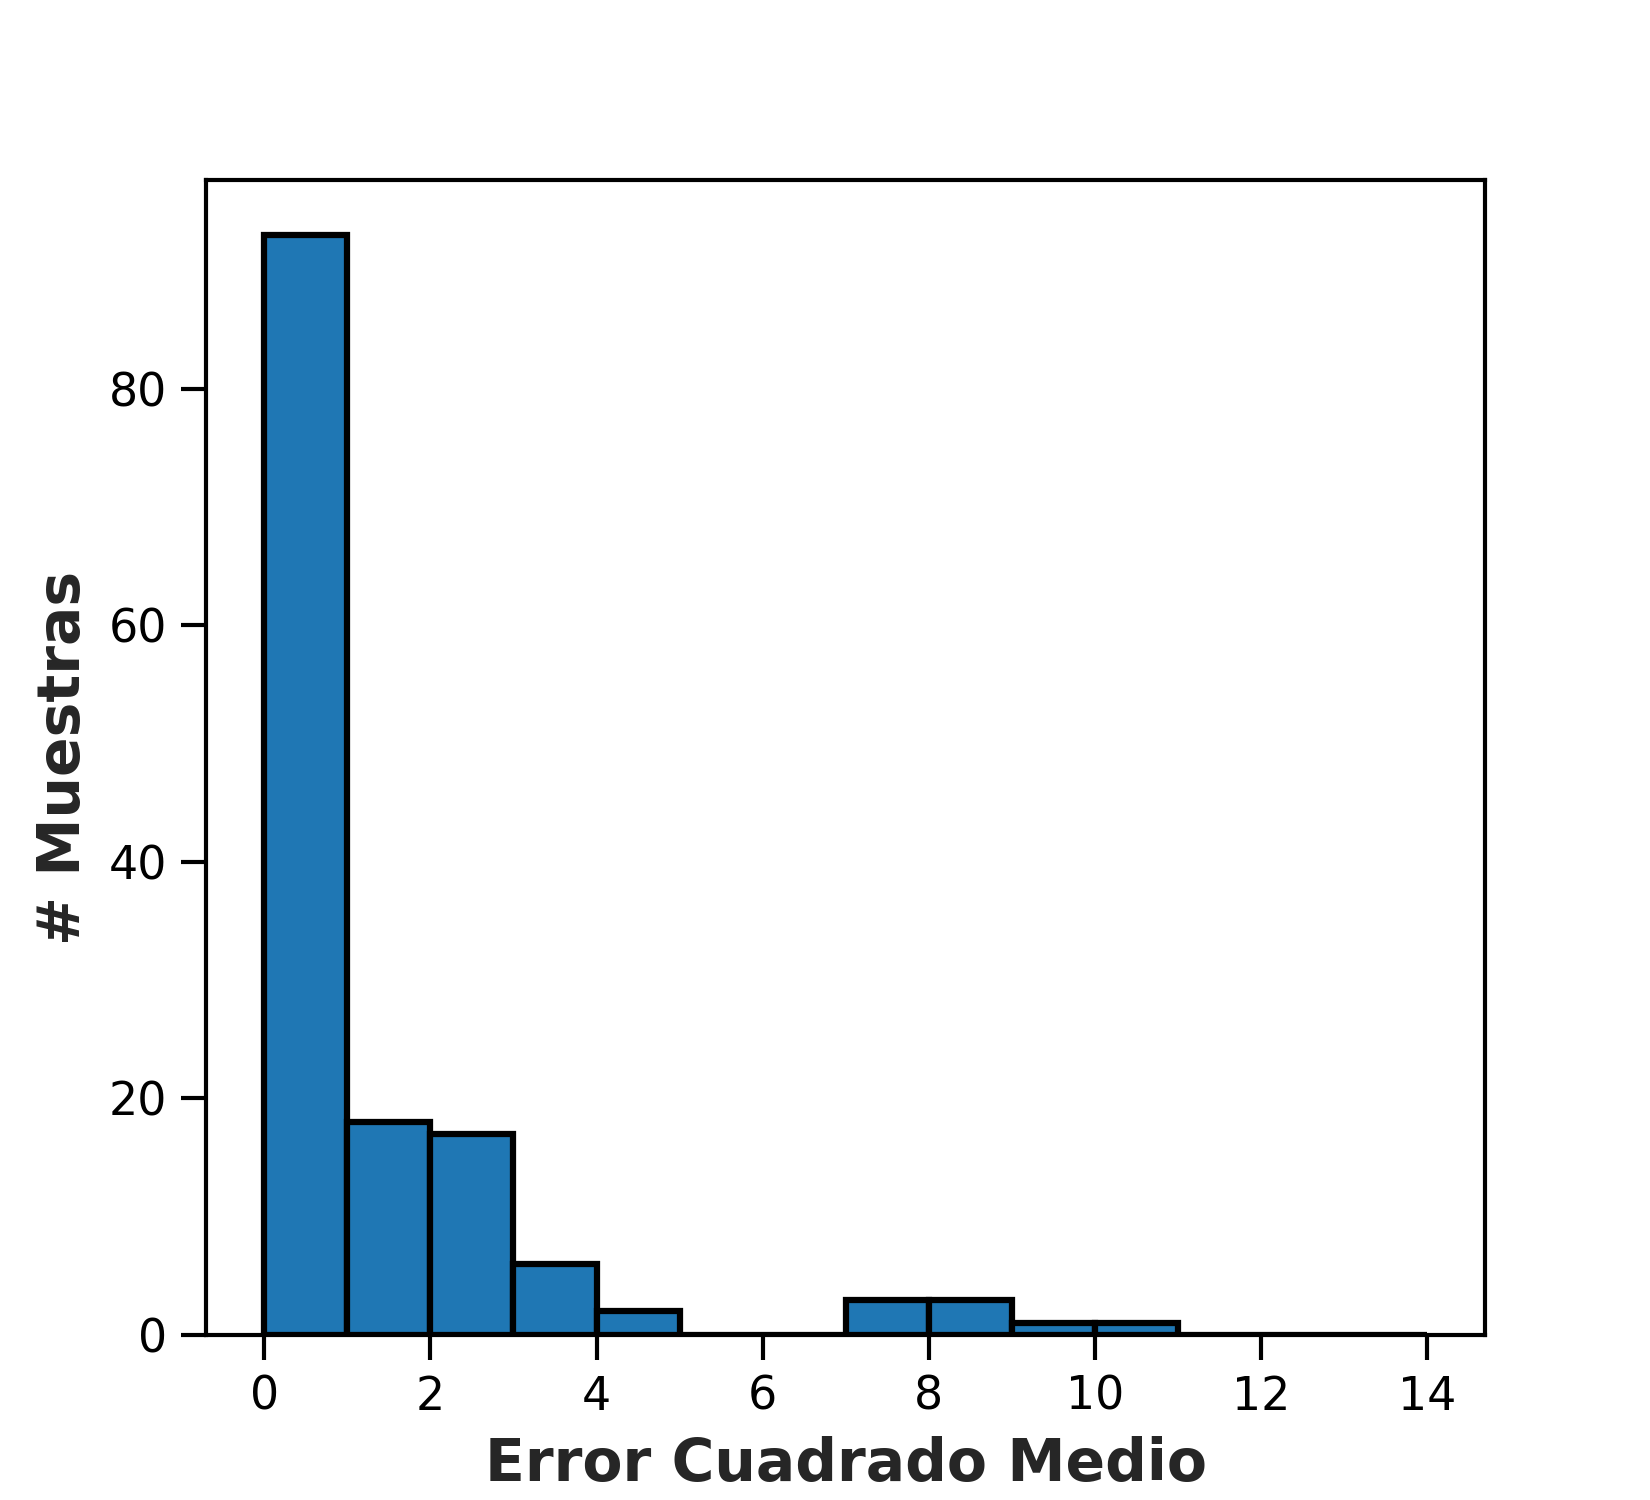
\includegraphics[width=0.7\textwidth]{ECM_DE.png}
\caption{Histograma del MSE del ajuste DE.}
\label{fig:ecm-de}
\end{figure}

\begin{figure}[htbp]
\centering
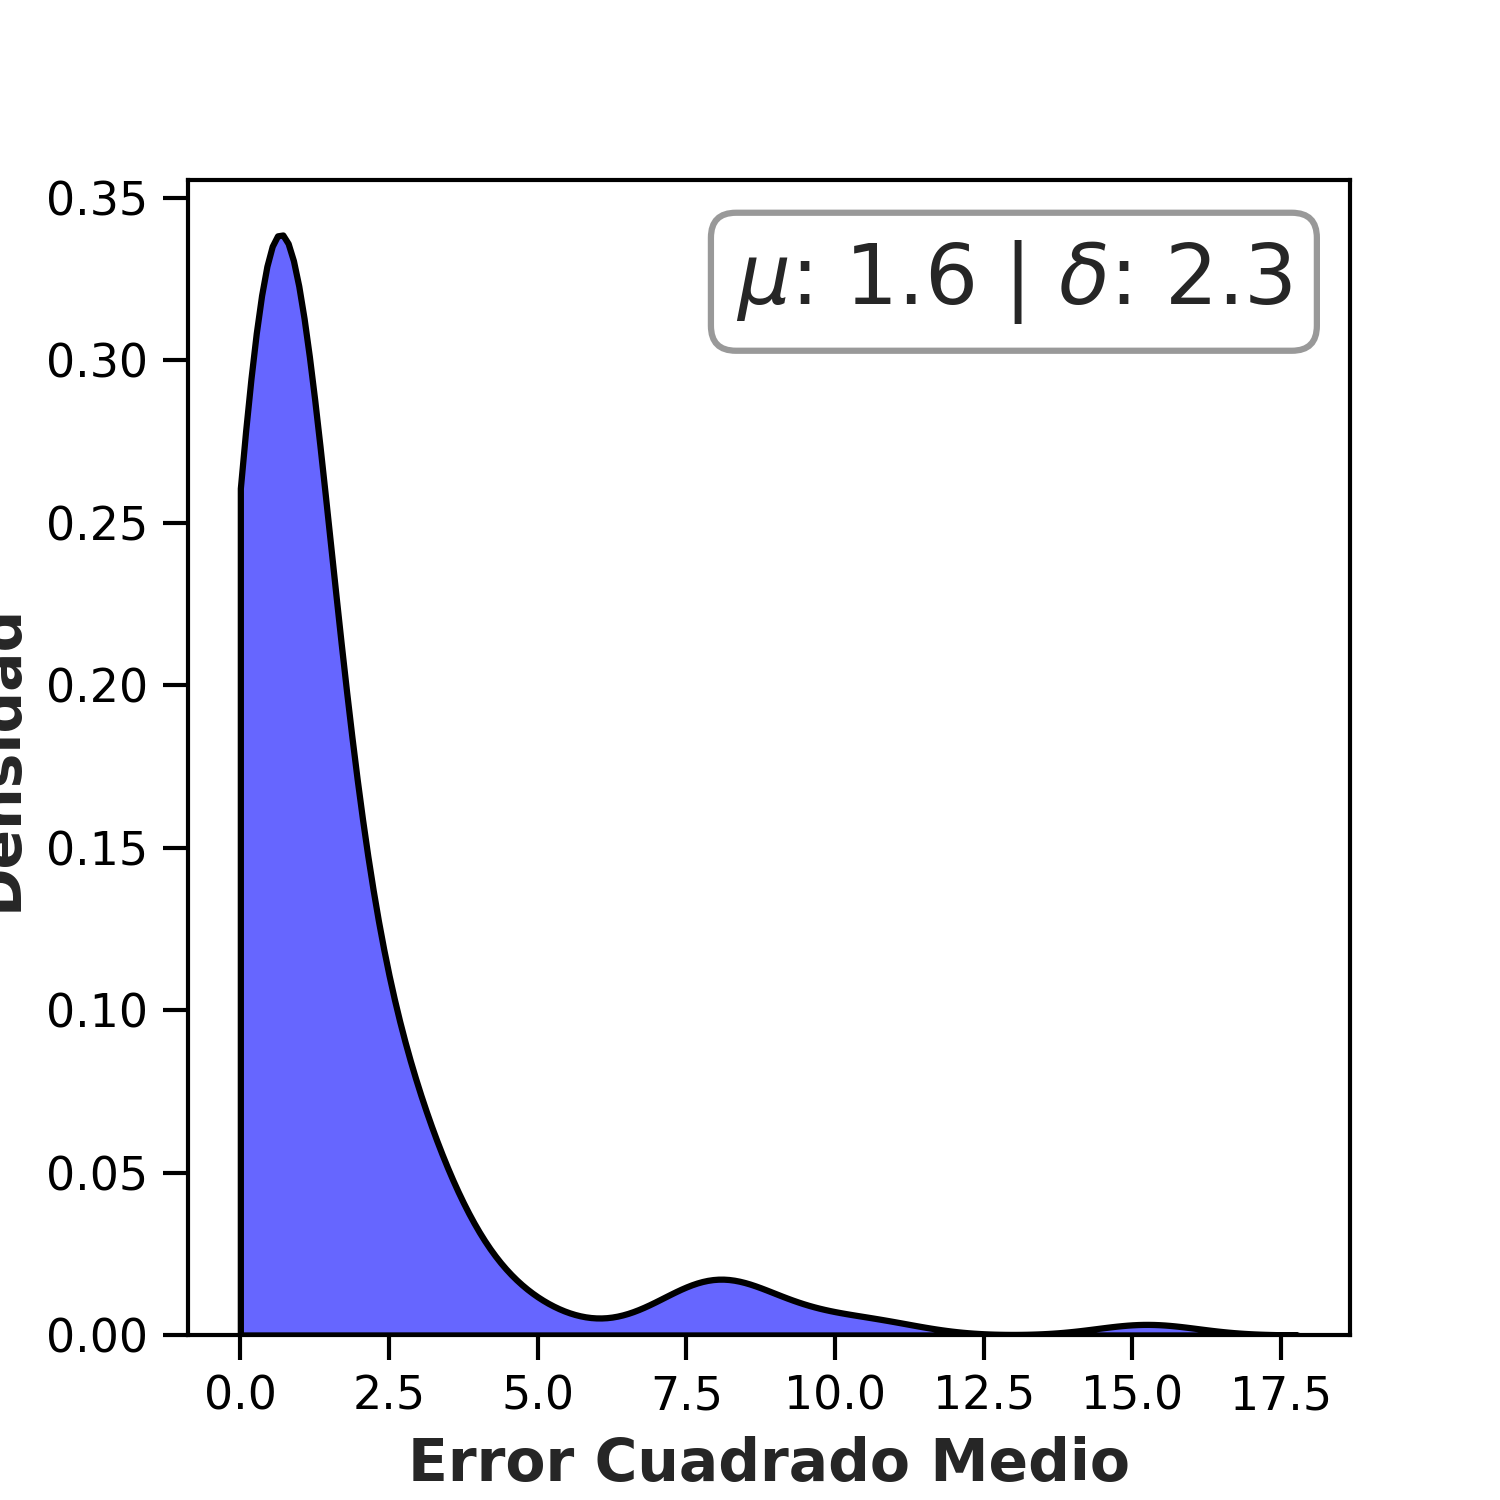
\includegraphics[width=0.7\textwidth]{error_kde.png}
\caption{Densidad KDE del error MSE con anotaciones de $\mu$ y $\delta$.}
\label{fig:error-kde}
\end{figure}

\begin{figure}[htbp]
\centering
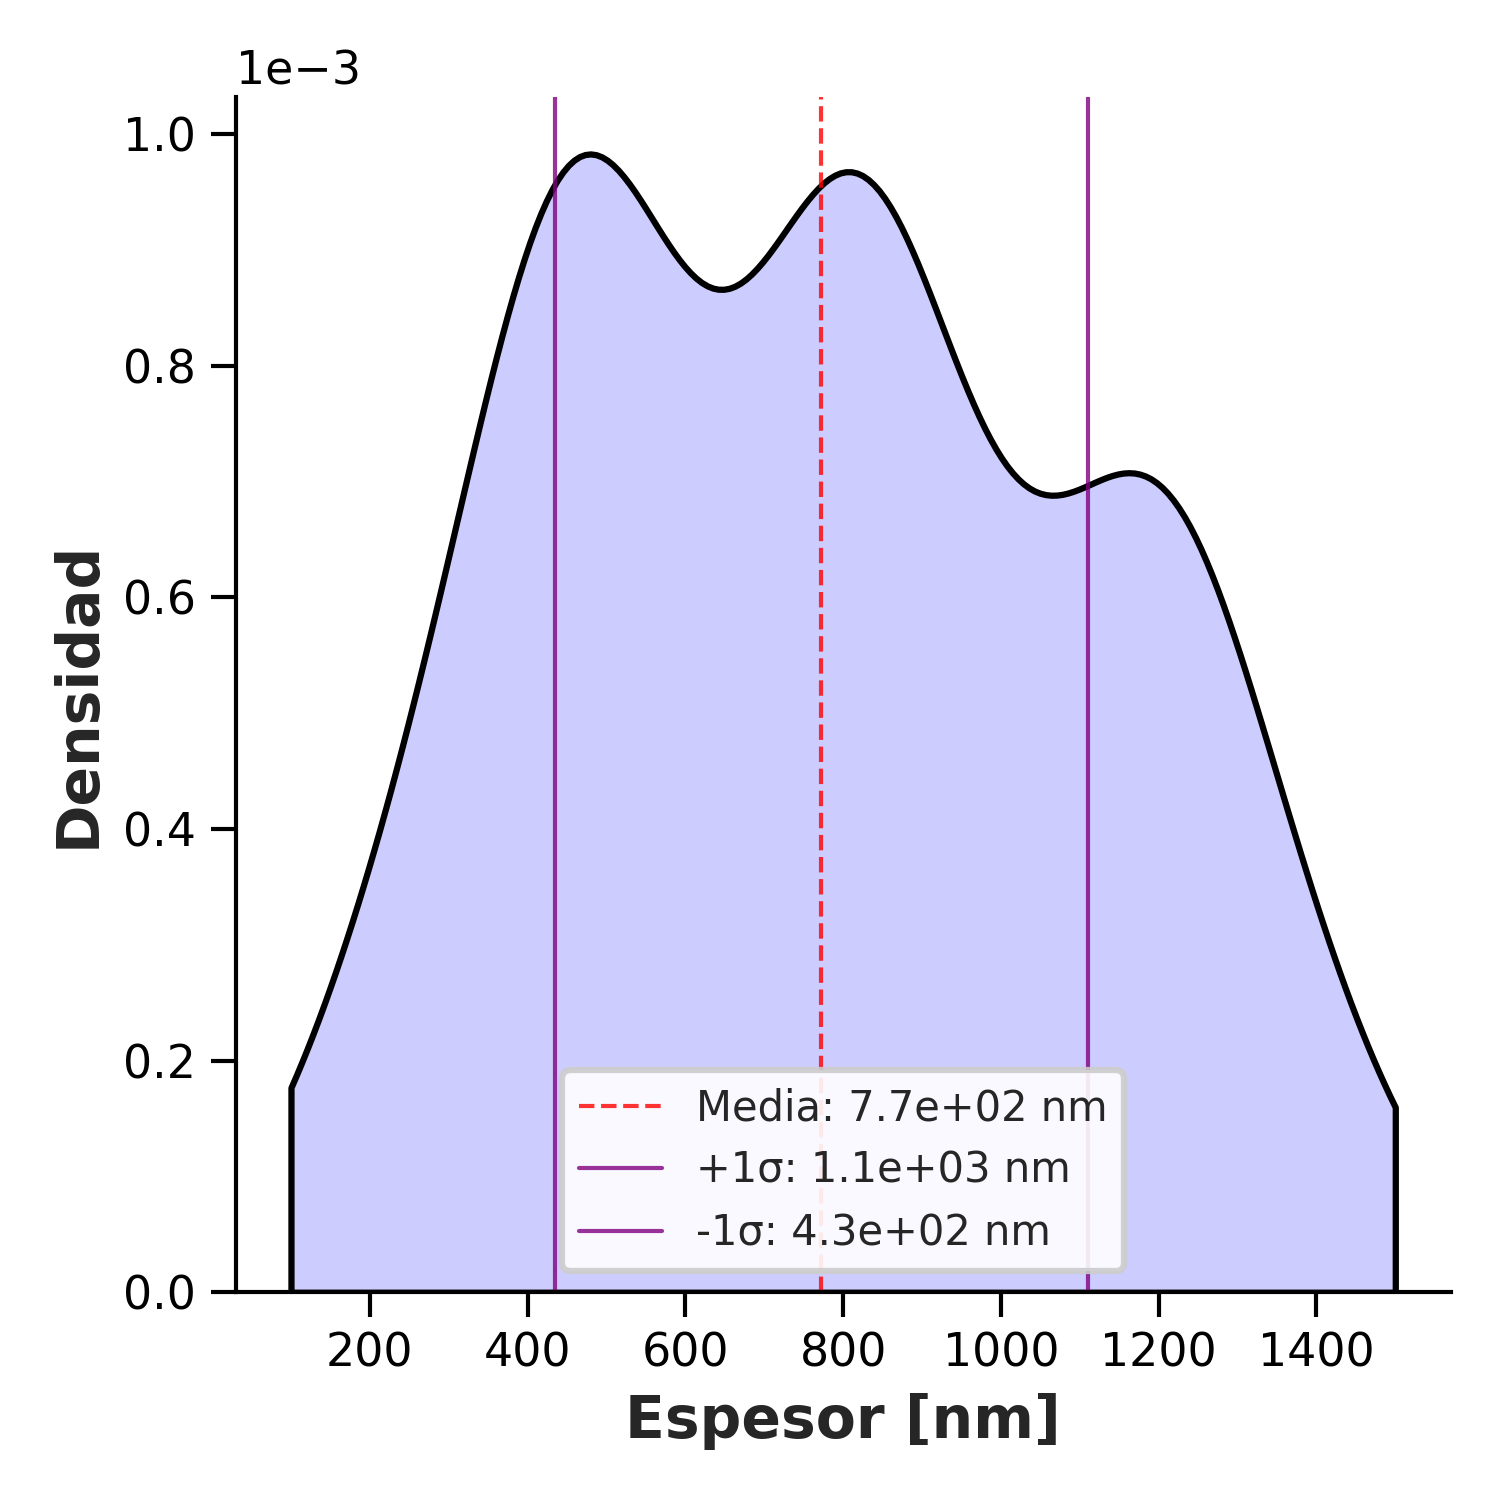
\includegraphics[width=0.7\textwidth]{thickness_kde.png}
\caption{Densidad KDE de la distribuci\'on de espesores.}
\label{fig:thickness-kde}
\end{figure}

% Grid samples
\begin{figure}[htbp]
\centering
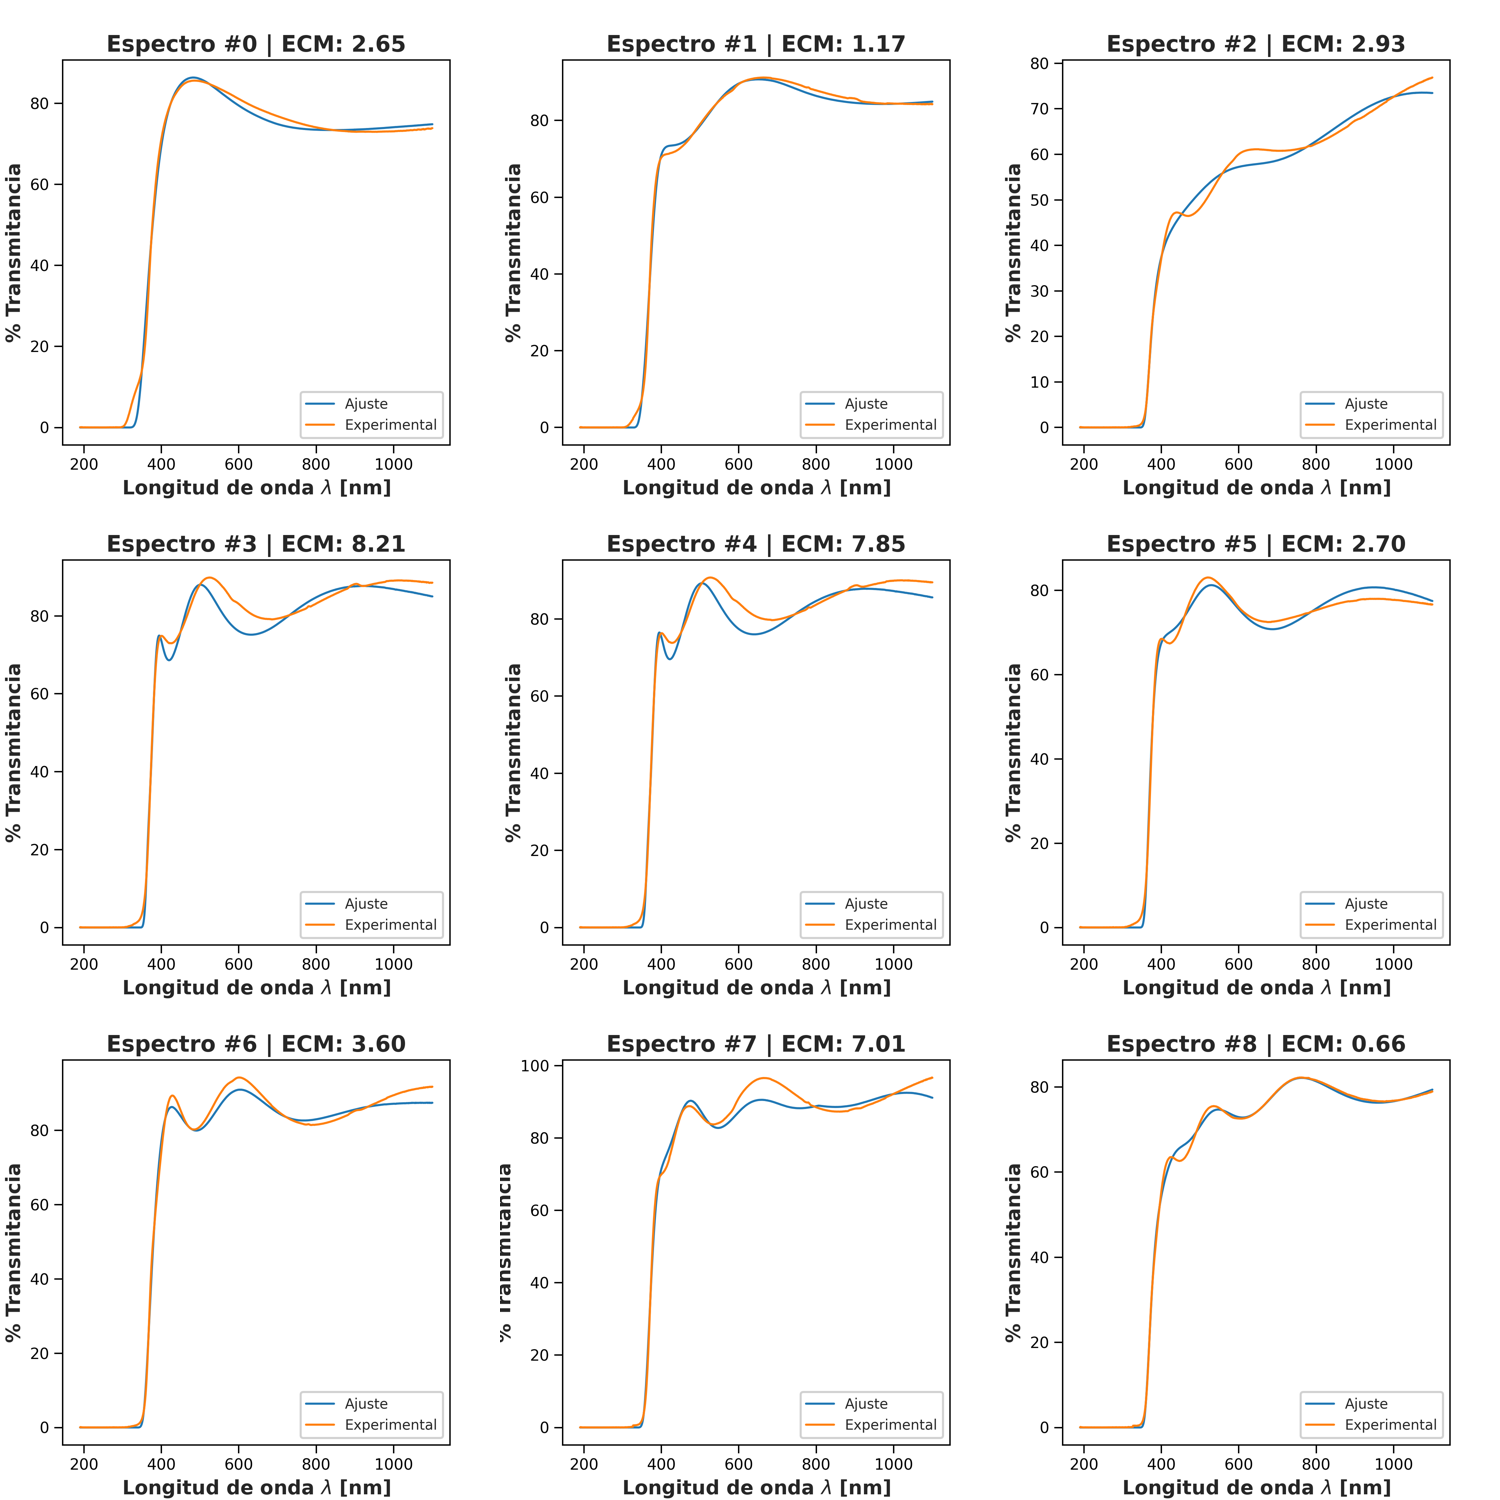
\includegraphics[width=0.85\textwidth]{grid_0.png}
\caption{Cuadr\'icula $3 \times 3$ de comparaci\'on de espectros (Grid 0).}
\label{fig:grid0}
\end{figure}

\begin{figure}[htbp]
\centering
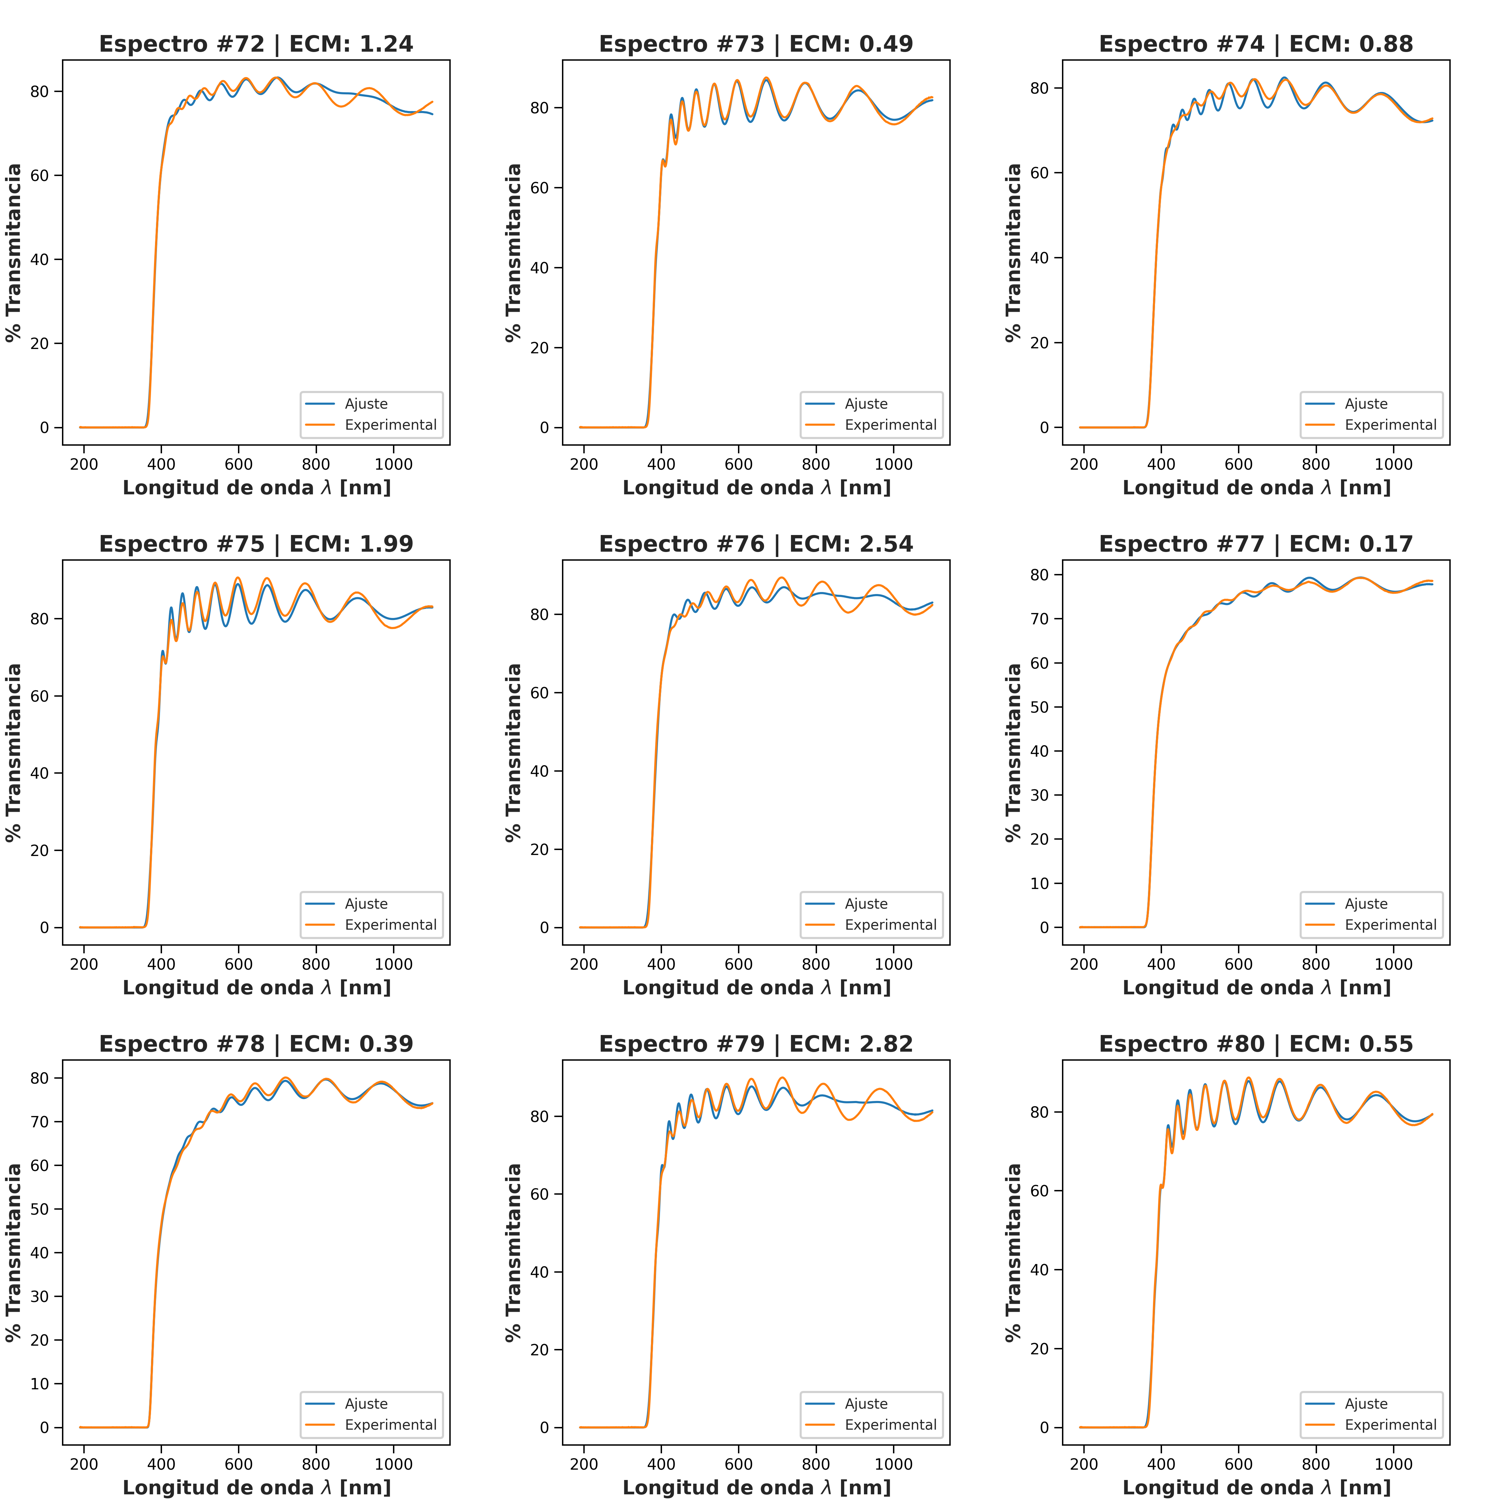
\includegraphics[width=0.85\textwidth]{grid_8.png}
\caption{Cuadr\'icula $3 \times 3$ de comparaci\'on de espectros (Grid 8).}
\label{fig:grid8}
\end{figure}

\begin{figure}[htbp]
\centering
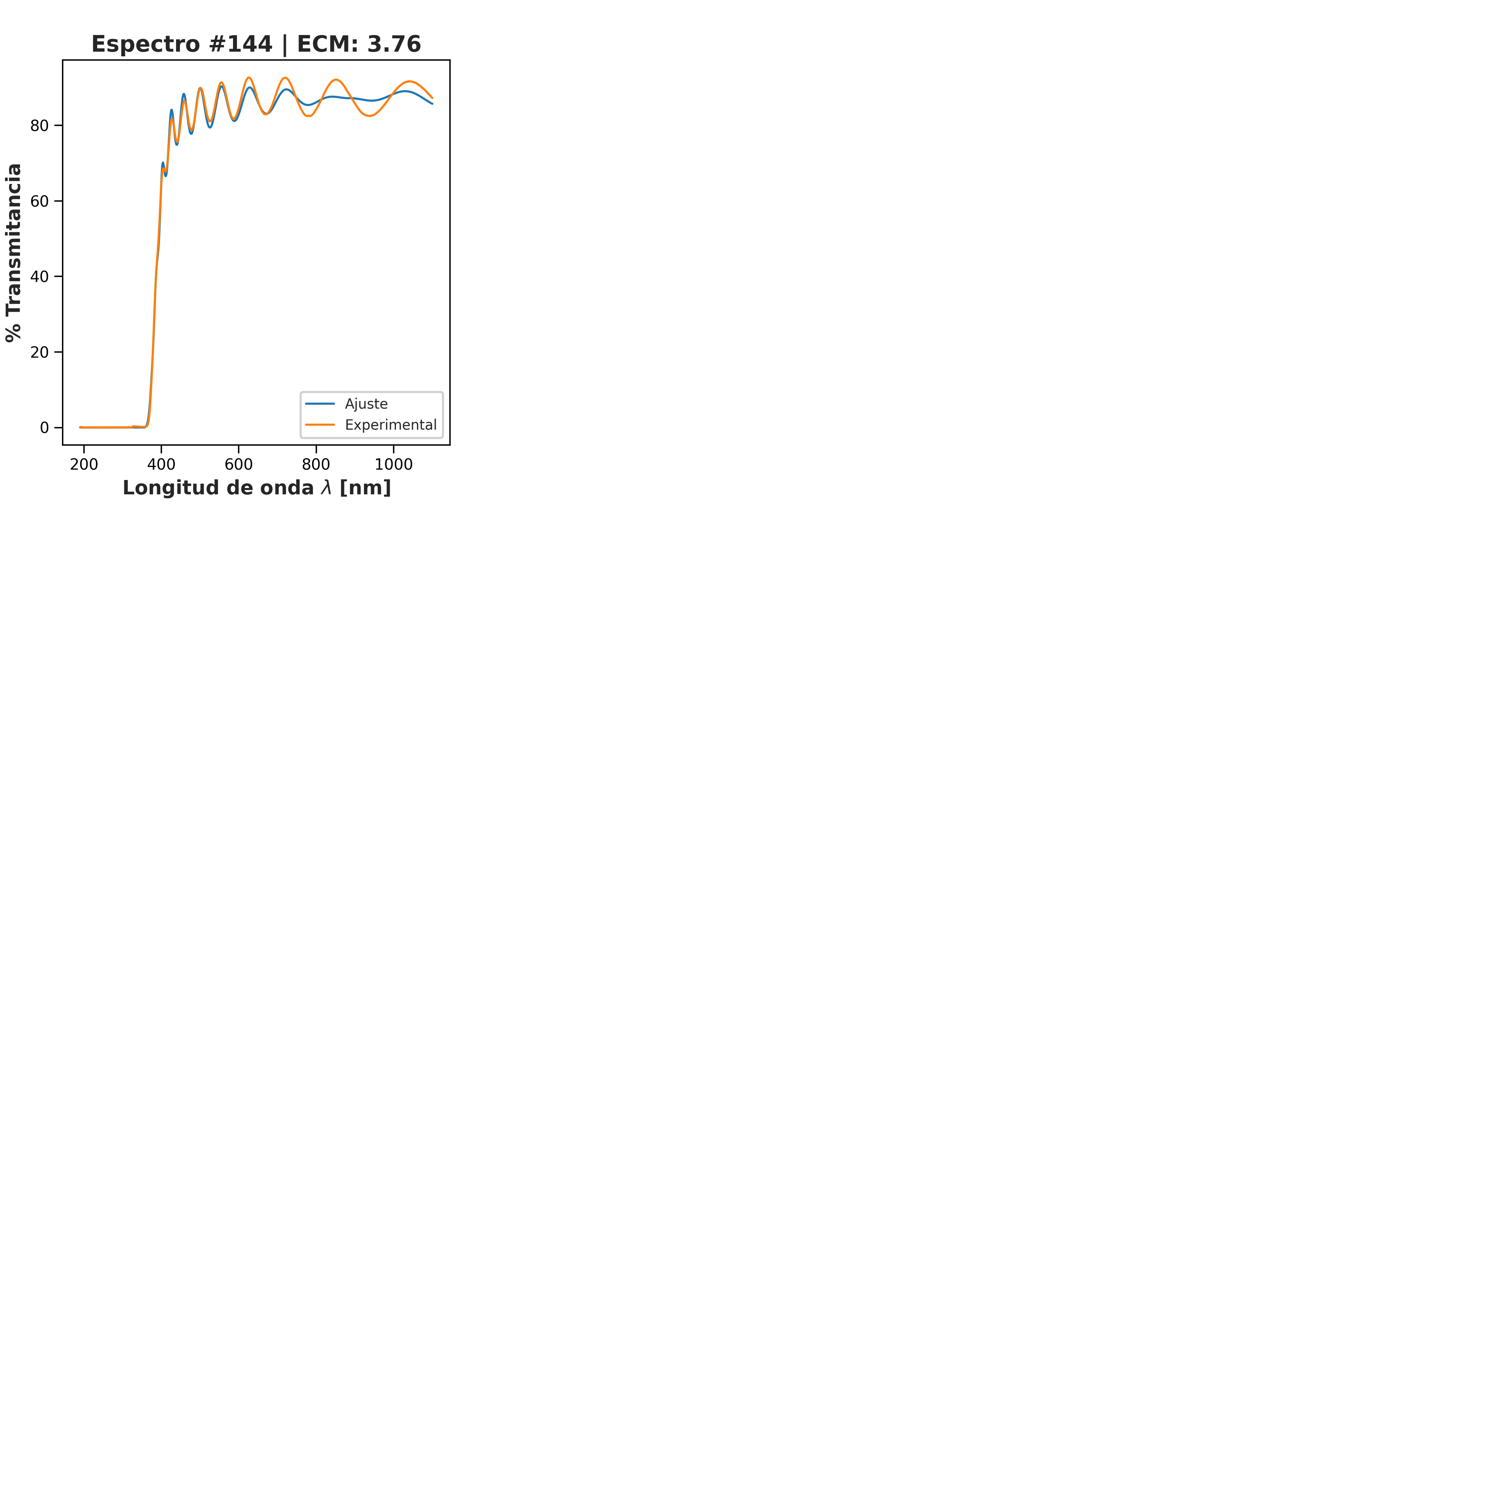
\includegraphics[width=0.85\textwidth]{grid_16.png}
\caption{Cuadr\'icula $3 \times 3$ de comparaci\'on de espectros (Grid 16, \'ultima).}
\label{fig:grid16}
\end{figure}

% Diagnostic figures
\begin{figure}[htbp]
\centering
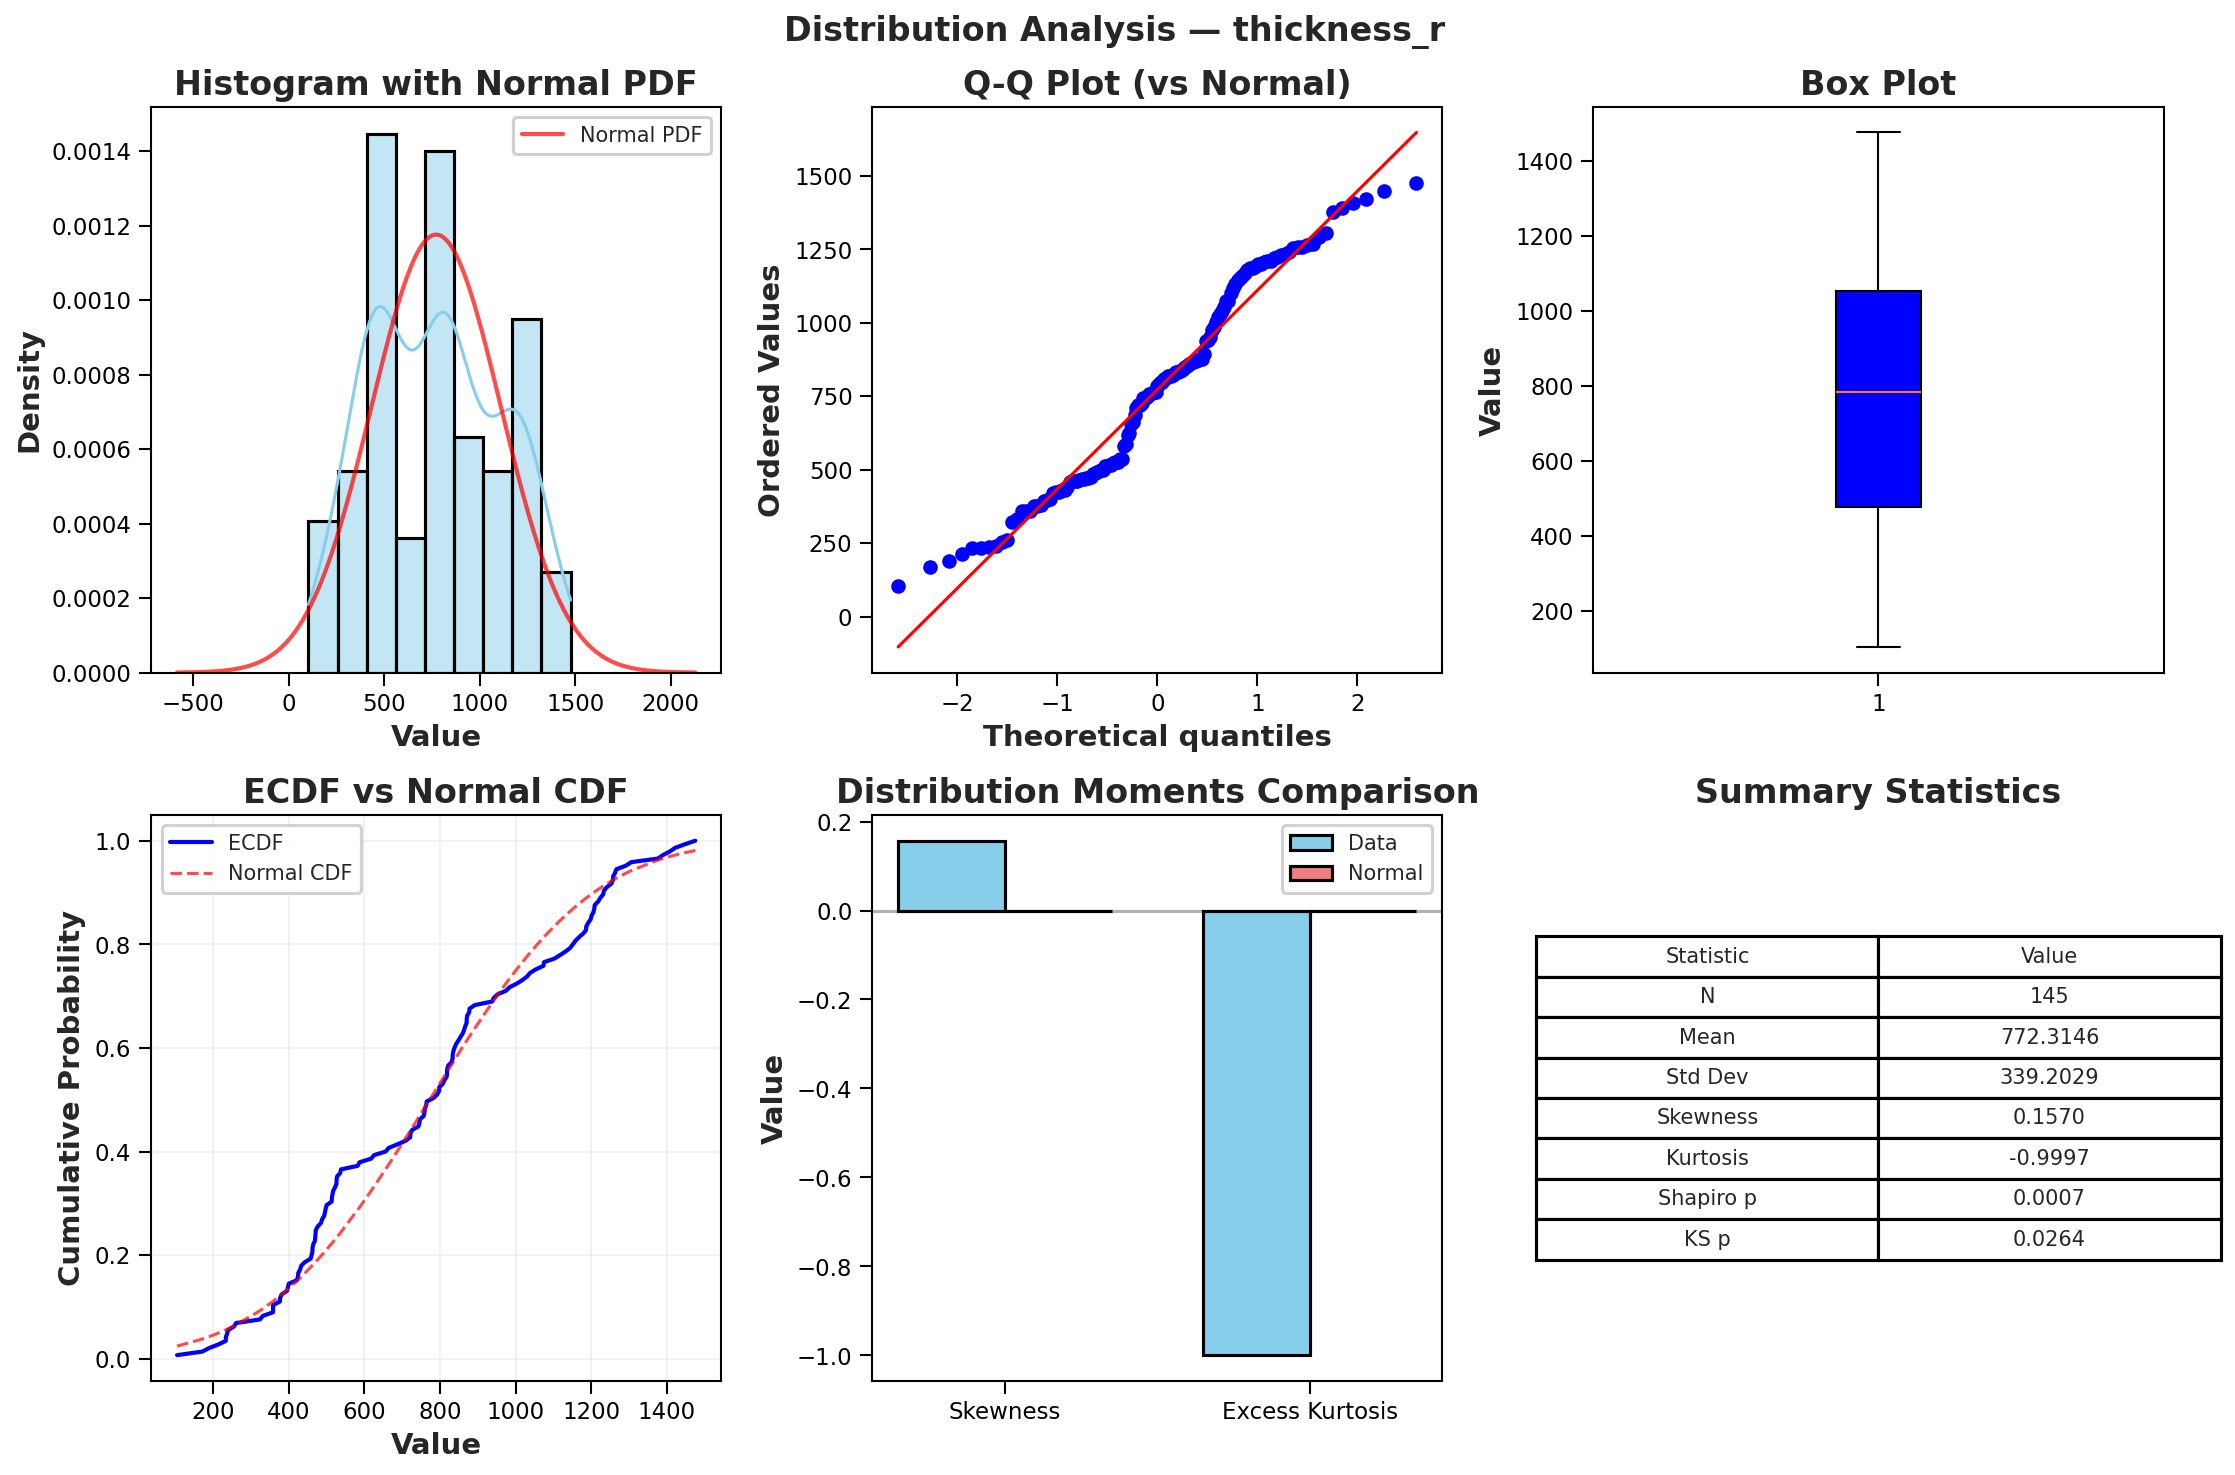
\includegraphics[width=0.85\textwidth]{analysis_thickness_r.png}
\caption{An\'alisis diagn\'ostico de 6 paneles para el par\'ametro de espesor ($d$).}
\label{fig:analysis-d}
\end{figure}

\begin{figure}[htbp]
\centering
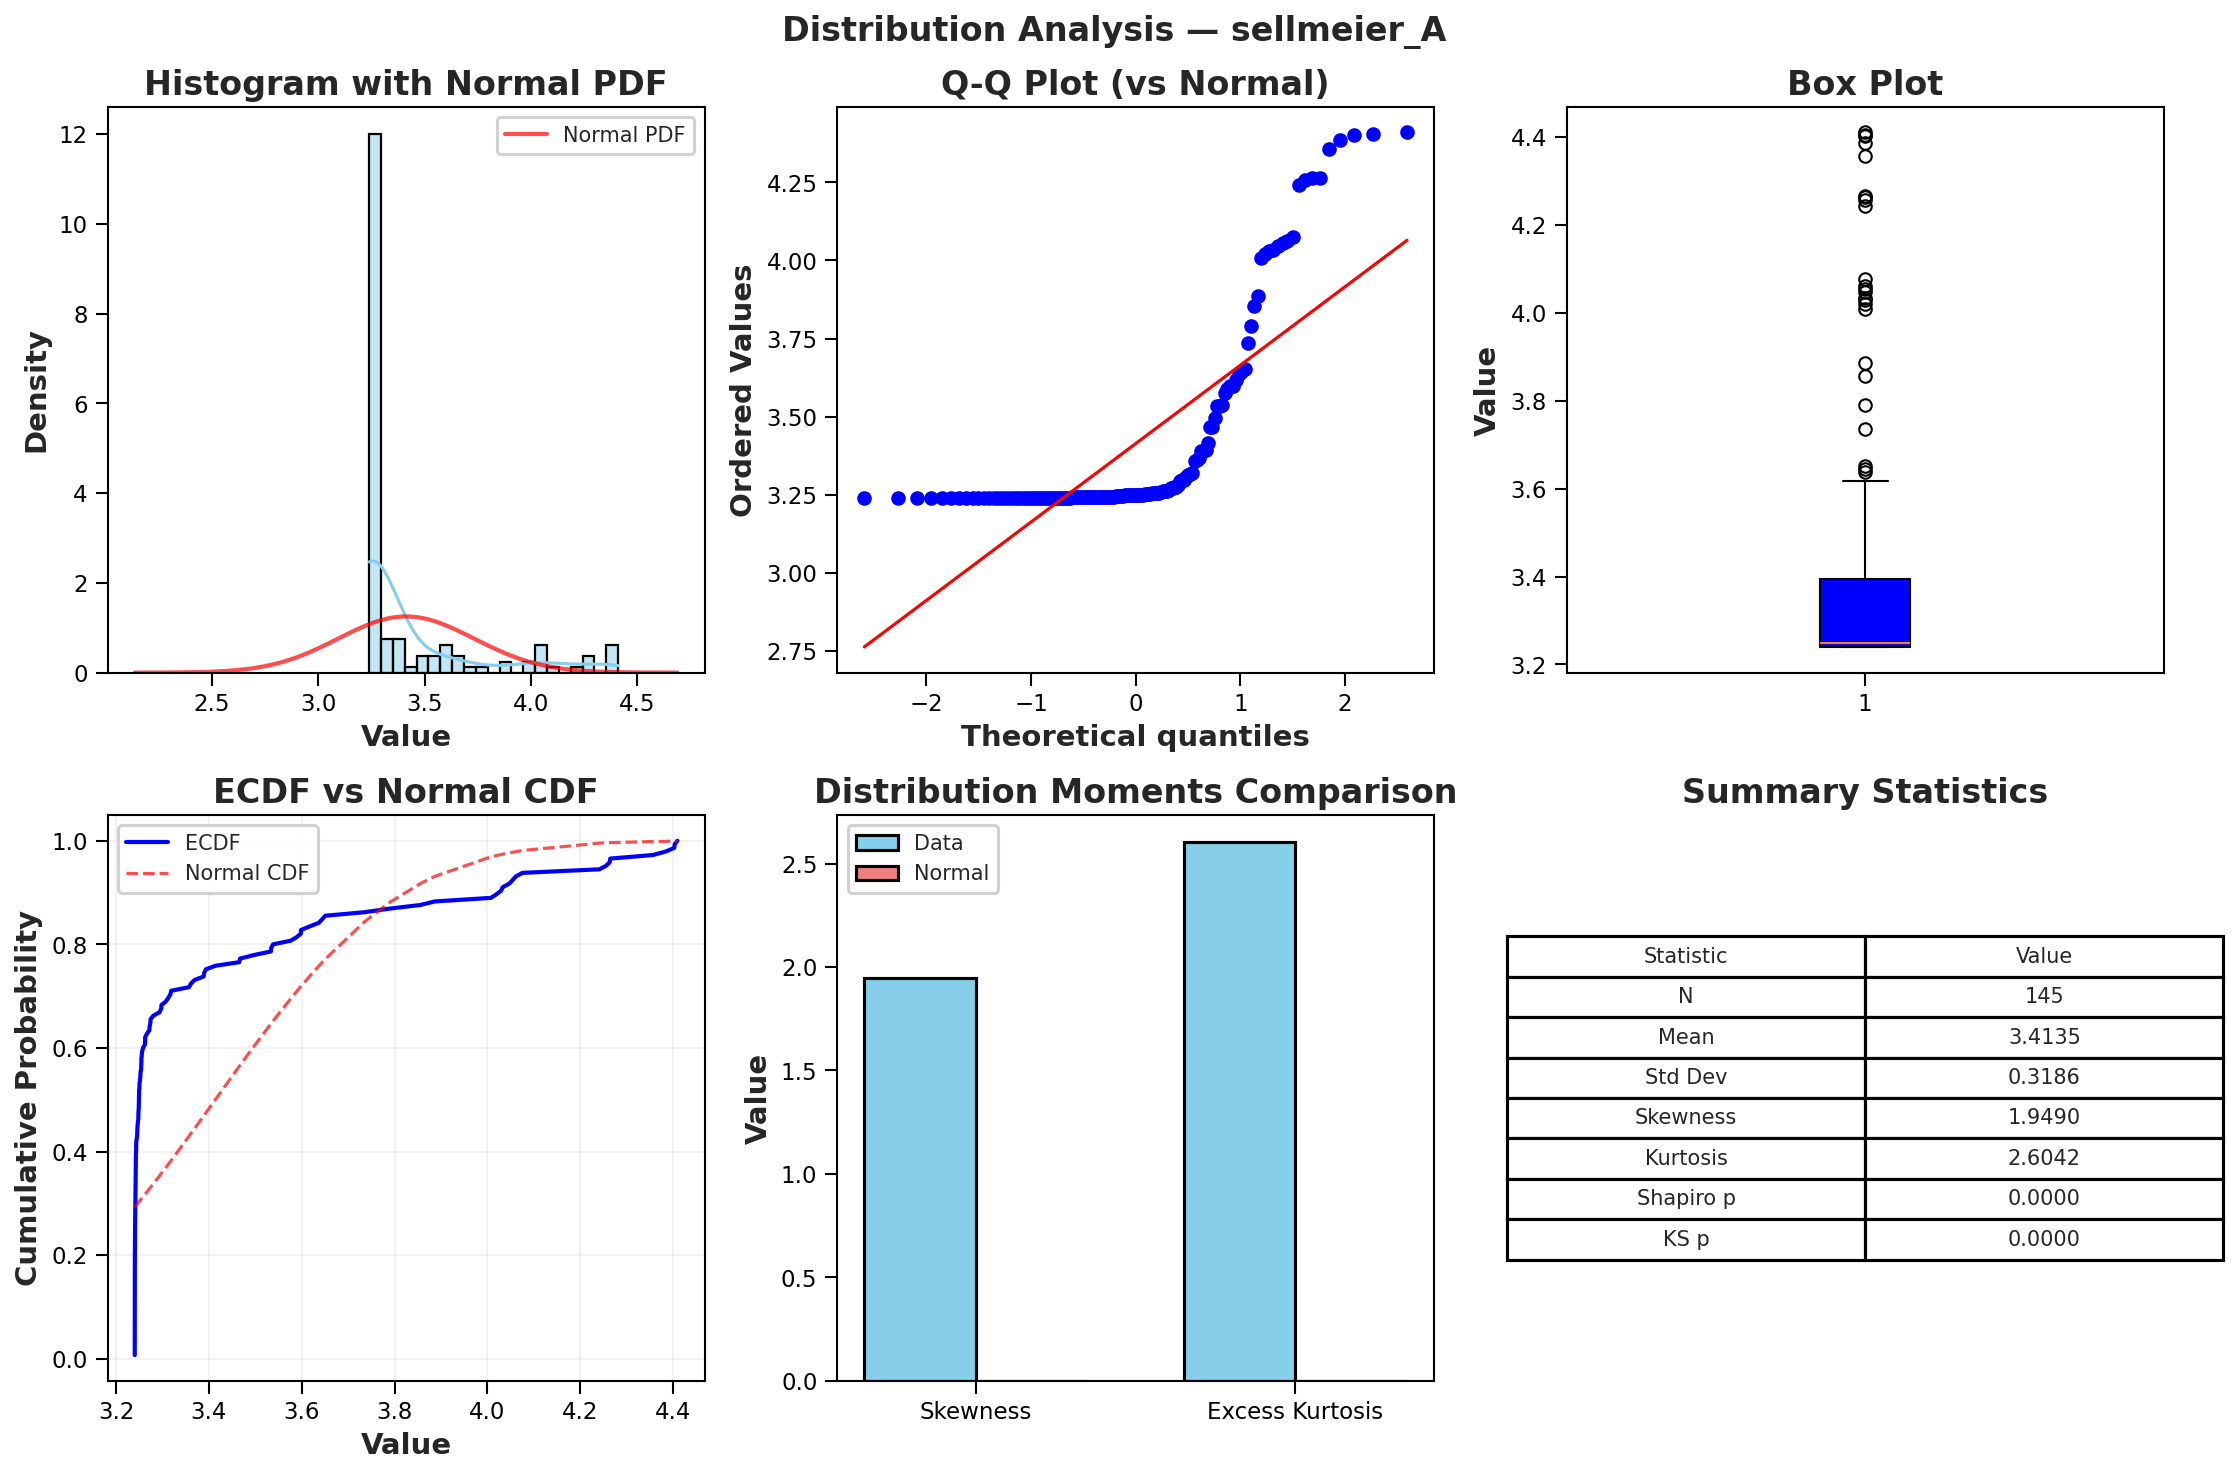
\includegraphics[width=0.85\textwidth]{analysis_sellmeier_A.png}
\caption{An\'alisis diagn\'ostico de 6 paneles para el par\'ametro Sellmeier $A$.}
\label{fig:analysis-A}
\end{figure}

% Ridge composites
\begin{figure}[htbp]
\centering

\includegraphics[width=\textwidth]{combined_rugosidades.png}
\caption{Gr\'aficos de cresta combinados: espesor, $\sigma_1$, $\sigma_2$ ($1 \times 3$).}
\label{fig:ridge-rug}
\end{figure}

\begin{figure}[htbp]
\centering

\includegraphics[width=\textwidth]{combined_sellmeier.png}
\caption{Gr\'aficos de cresta combinados: Sellmeier $A, B, C, D, E$ y $n(\lambda)$ ($2 \times 3$).}
\label{fig:ridge-sell}
\end{figure}

\begin{figure}[htbp]
\centering

\includegraphics[width=\textwidth]{combined_absorcion.png}
\caption{Gr\'aficos de cresta combinados: $\alpha_0, \beta, \lambda_g, n_e$ ($2 \times 2$).}
\label{fig:ridge-abs}
\end{figure}

% ============================================================
% CHAPTER 3: Simulación de Datos Sintéticos mediante GMM
% ============================================================
\section{Simulaci\'on de Datos Sint\'eticos mediante Modelos de Mezcla Gaussiana}
\label{sec:data-sim}

\subsection{Descripci\'on General del Pipeline}

La generaci\'on de datos sint\'eticos constituye un componente cr\'itico del proyecto AzONetV2, ya que el conjunto experimental de 145 muestras resulta insuficiente para entrenar una red neuronal profunda tipo U-NET. El pipeline completo de simulaci\'on comprende las siguientes etapas:

\begin{enumerate}
    \item \textbf{Preparaci\'on}: Organizaci\'on de los par\'ametros DE en 5 regiones de espesor.
    \item \textbf{Ajuste GMM}: Modelado de cada par\'ametro con Modelos de Mezcla Gaussiana (GMM), seleccionando el n\'umero \'optimo de componentes mediante el criterio BIC.
    \item \textbf{Generaci\'on de par\'ametros}: Muestreo de 3000 valores por par\'ametro en cada regi\'on, con filtro de rechazo para las tuplas de Sellmeier que violan $1.8 \leq n(\lambda) \leq 2.1$.
    \item \textbf{C\'alculo de espectros}: Para $\sim$240,000 iteraciones por regi\'on, se selecciona independientemente un valor de cada par\'ametro y se calcula el espectro de transmitancia de 911 puntos mediante el modelo de Alonso.
    \item \textbf{Validaci\'on}: Comparaci\'on visual de distribuciones originales vs simuladas mediante gr\'aficos de cresta, espectros de muestra e histogramas de espesor.
    \item \textbf{Uni\'on y partici\'on}: Concatenaci\'on de los 5 archivos Parquet en un \'unico conjunto de $\sim$1.2M de espectros, y divisi\'on 80/10/10 en archivos HDF5.
\end{enumerate}

El volumen total de datos generados es de $\sim 1,200,000$ espectros (5 regiones $\times \sim 240,000$ espectros), cada uno con 911 puntos de longitud de onda y su correspondiente espesor.

\subsection{Archivos Fuente}

Los scripts que implementan este pipeline son:
\begin{itemize}
    \item \texttt{bin\_\{0,1,2,3,4\}.py}: Scripts individuales para cada una de las 5 regiones de espesor.
    \item \texttt{2\_Figures\_Colab.py}: Generaci\'on de figuras de validaci\'on.
    \item \texttt{3\_join\_split\_merge\_Colab.py}: Concatenaci\'on, mezcla y partici\'on del conjunto final.
\end{itemize}

El modelo de Alonso fue re-implementado para esta fase, retornando no solo el espectro de transmitancia sino tambi\'en todos los par\'ametros intermedios (\'indices de refracci\'on, coeficientes de absorci\'on, correcciones de rugosidad, etc.).

\subsection{Fase 1: Ajuste de Modelos de Mezcla Gaussiana}

\subsubsection{Datos de Entrada}

Cada archivo \texttt{region\_\{bint\}.npy} contiene una matriz de dimensiones $(n_{\text{muestras}}, 13)$ con los siguientes par\'ametros en orden:

\[
[d,\; R_1,\; R_2,\; A,\; B,\; C,\; D,\; E,\; \alpha_0,\; \beta,\; \lambda_g,\; n_e,\; \text{MSE}]
\]

\subsubsection{Procedimiento GMM}

Para cada regi\'on de espesor:
\begin{enumerate}
    \item Se ajusta un GMM a los datos de cada par\'ametro individual con \texttt{max\_gaussians = 10}, seleccionando el n\'umero \'optimo de componentes $K_{\text{opt}}$ mediante minimizaci\'on del criterio BIC (\textit{Bayesian Information Criterion}).
    \item Para los par\'ametros de Sellmeier ($A, B, C, D, E$), se aplica un m\'aximo de 3 componentes Gaussianas (\texttt{max\_gaussians = 3}) para mantener la parsimonia del modelo.
    \item De cada GMM ajustado se generan 3000 nuevos valores mediante muestreo aleatorio.
    \item Para los 5 par\'ametros de Sellmeier, se aplica un filtro de rechazo: solo se conservan las tuplas $(A, B, C, D, E)$ que producen un \'indice de refracci\'on $n(\lambda)$ en el rango f\'isicamente v\'alido $1.8 \leq n(\lambda) \leq 2.1$ para todo $\lambda \in [190, 1100]$ nm.
\end{enumerate}

\subsection{Fase 2: Generaci\'on de Espectros de Transmitancia}

Para cada regi\'on, se ejecutan $\sim 240,000$ iteraciones. En cada iteraci\'on:
\begin{enumerate}
    \item Se selecciona aleatoria e independientemente un valor de cada uno de los 13 par\'ametros del \textit{pool} de 3000 valores generados por el GMM.
    \item Se invoca la funci\'on \texttt{modelo\_transmitancia} con 911 puntos de longitud de onda ($\lambda$).
    \item Los espectros que resultan en valores \texttt{NaN} (debido a inestabilidades num\'ericas en casos extremos) son descartados.
    \item El \textit{DataFrame} resultante se mezcla aleatoriamente (\textit{shuffle}) antes de guardarse en formato Parquet.
\end{enumerate}

\subsection{Fase 3: Figuras de Validaci\'on}

El script \texttt{2\_Figures\_Colab.py} genera las siguientes visualizaciones de validaci\'on:

\begin{itemize}
    \item \textbf{Gr\'aficos de cresta (\textit{ridge plots})}: 5 filas por par\'ametro, donde la distribuci\'on original (resultados DE) se muestra en azul ($\rho$) y la distribuci\'on simulada (GMM) en rojo ($\rho_s$).
    \item \textbf{Muestras de espectros}: Espectros de transmitancia simulados representativos de las regiones R$_1$, R$_3$ y R$_5$.
    \item \textbf{Histogramas de espesor}: Comparaci\'on de la distribuci\'on de espesores simulados vs originales.
\end{itemize}

\subsection{Fase 4: Uni\'on y Partici\'on del Conjunto Final}

\subsubsection{Esquema del Archivo Parquet}

Los 5 archivos Parquet (uno por regi\'on) se concatenan para formar \texttt{Final\_Dataset.parquet}, con $\sim 1,200,000$ filas. El Cuadro~\ref{tab:parquet-schema} muestra el esquema de columnas.

\begin{table}[htbp]
\centering
\caption{Esquema del archivo Parquet \texttt{Final\_Dataset.parquet}.}
\label{tab:parquet-schema}
\begin{tabular}{@{}ccc@{}}
\toprule
\textbf{Columna} & \textbf{Tipo} & \textbf{Descripci\'on} \\
\midrule
\texttt{wl\_000}--\texttt{wl\_910} & \texttt{float32} & Transmitancia en 911 longitudes de onda \\
\texttt{thickness} & \texttt{float32} & Espesor de la pel\'icula (nm) \\
\bottomrule
\end{tabular}
\end{table}

\subsubsection{Esquema de los Archivos HDF5}

El conjunto se divide en tres particiones ML-ready: 80\% entrenamiento, 10\% validaci\'on, 10\% prueba. Los datos se almacenan en formato HDF5 con el esquema descrito en el Cuadro~\ref{tab:hdf5-schema}.

\begin{table}[htbp]
\centering
\caption{Esquema de los datasets HDF5.}
\label{tab:hdf5-schema}
\begin{tabular}{@{}lccc@{}}
\toprule
\textbf{Dataset HDF5} & \textbf{Dimensiones} & \textbf{Tipo} & \textbf{Descripci\'on} \\
\midrule
\texttt{train.h5} & & & \\
\quad \texttt{x\_total} & $(960000, 911, 1)$ & \texttt{float32} & Espectros de entrenamiento \\
\quad \texttt{y\_total} & $(960000, 1)$ & \texttt{float32} & Espesores de entrenamiento \\
\texttt{val.h5} & & & \\
\quad \texttt{x\_total} & $(120000, 911, 1)$ & \texttt{float32} & Espectros de validaci\'on \\
\quad \texttt{y\_total} & $(120000, 1)$ & \texttt{float32} & Espesores de validaci\'on \\
\texttt{test.h5} & & & \\
\quad \texttt{x\_total} & $(120000, 911, 1)$ & \texttt{float32} & Espectros de prueba \\
\quad \texttt{y\_total} & $(120000, 1)$ & \texttt{float32} & Espesores de prueba \\
\bottomrule
\end{tabular}
\end{table}

Todos los datasets HDF5 utilizan compresi\'on con \texttt{chunks = True} para lectura eficiente durante el entrenamiento.

\subsection{Figuras de Validaci\'on de la Simulaci\'on}

% Ridge validation figures
\begin{figure}[htbp]
\centering

\includegraphics[width=\textwidth]{combined_rugosidades.png}
\caption{Gr\'aficos de cresta de validaci\'on: espesor, $\sigma_1$, $\sigma_2$ --- original (azul) vs simulado (rojo).}
\label{fig:sim-rug}
\end{figure}

\begin{figure}[htbp]
\centering

\includegraphics[width=\textwidth]{combined_sellmeier.png}
\caption{Gr\'aficos de cresta de validaci\'on: Sellmeier --- original vs simulado.}
\label{fig:sim-sell}
\end{figure}

\begin{figure}[htbp]
\centering

\includegraphics[width=\textwidth]{combined_absorcion.png}
\caption{Gr\'aficos de cresta de validaci\'on: par\'ametros de absorci\'on y $n_e$ --- original vs simulado.}
\label{fig:sim-abs}
\end{figure}

% Spectrum samples
\begin{figure}[htbp]
\centering
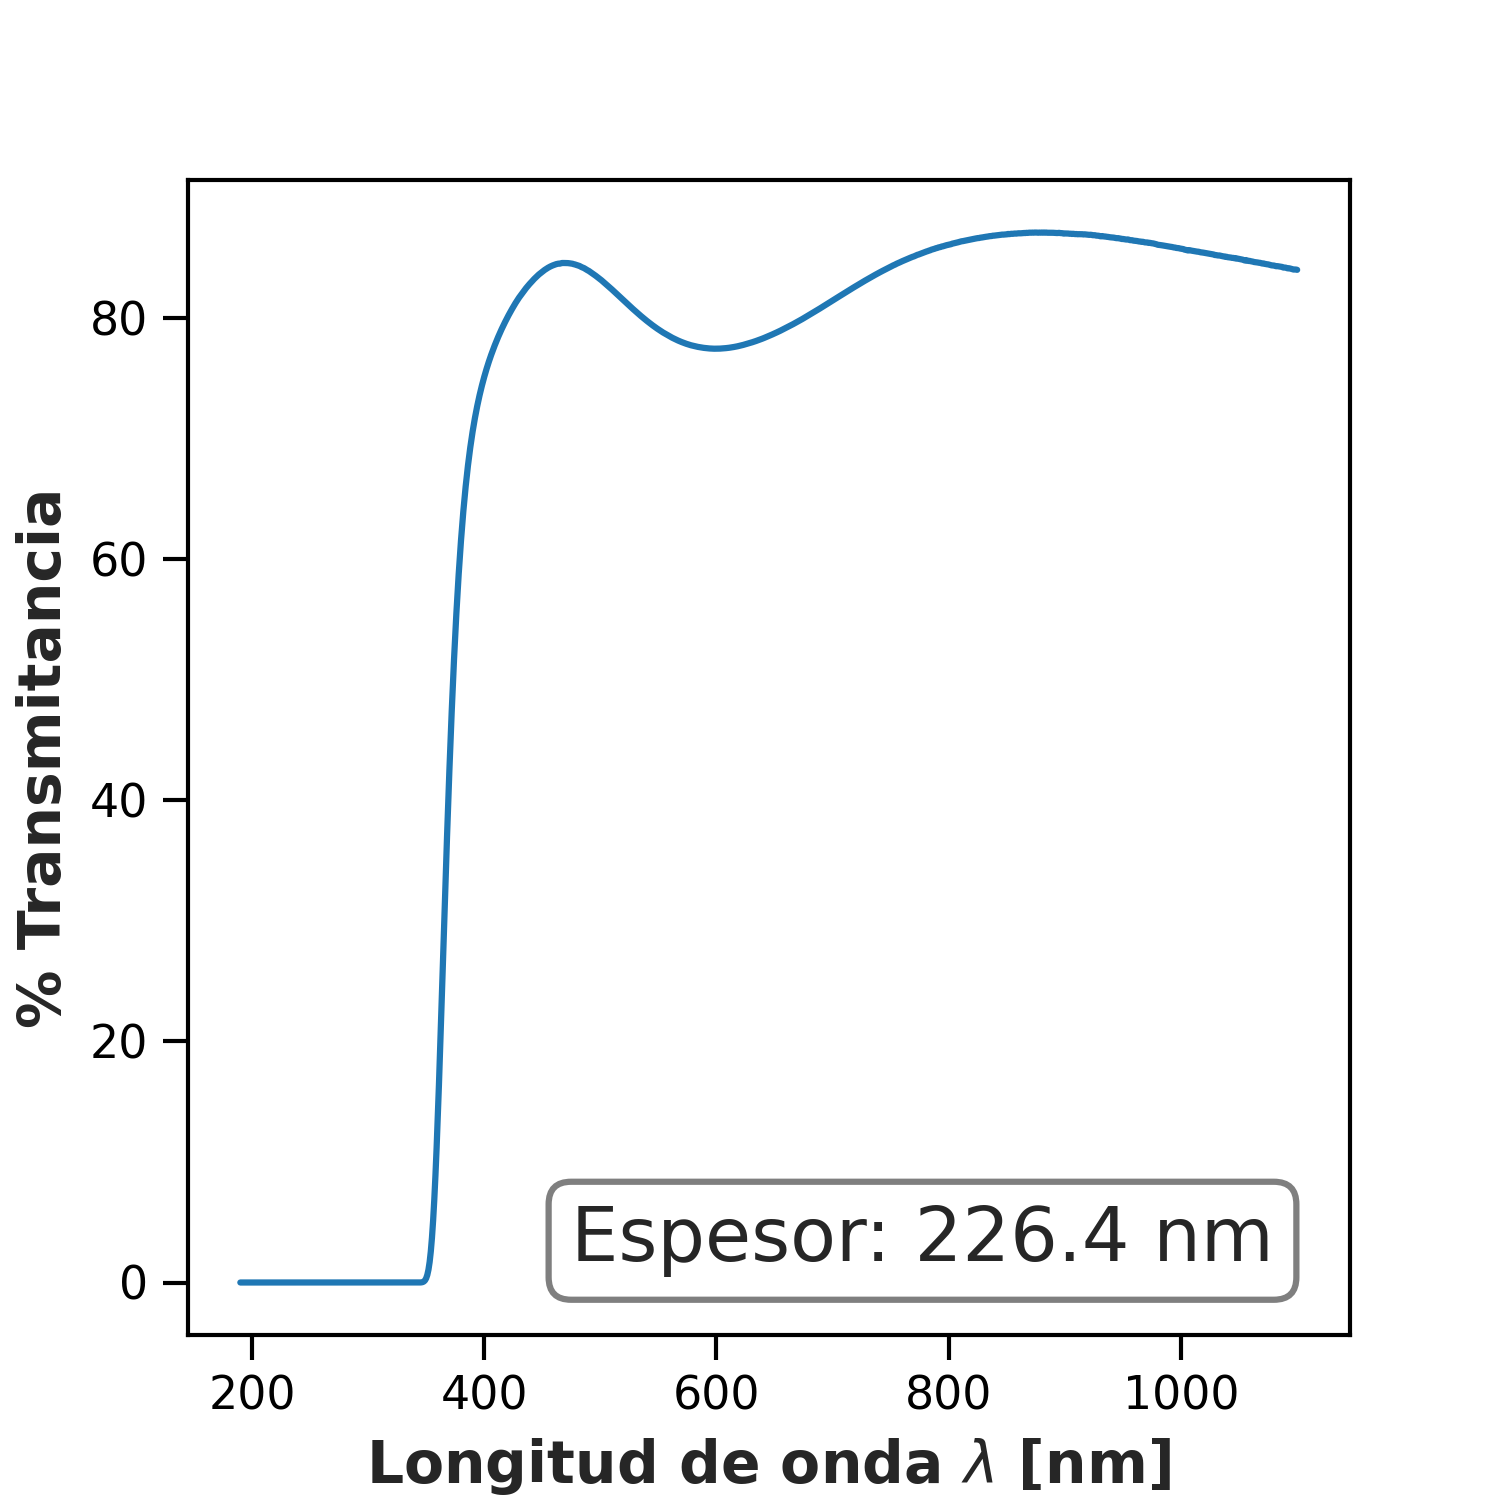
\includegraphics[width=0.48\textwidth]{r1.png}
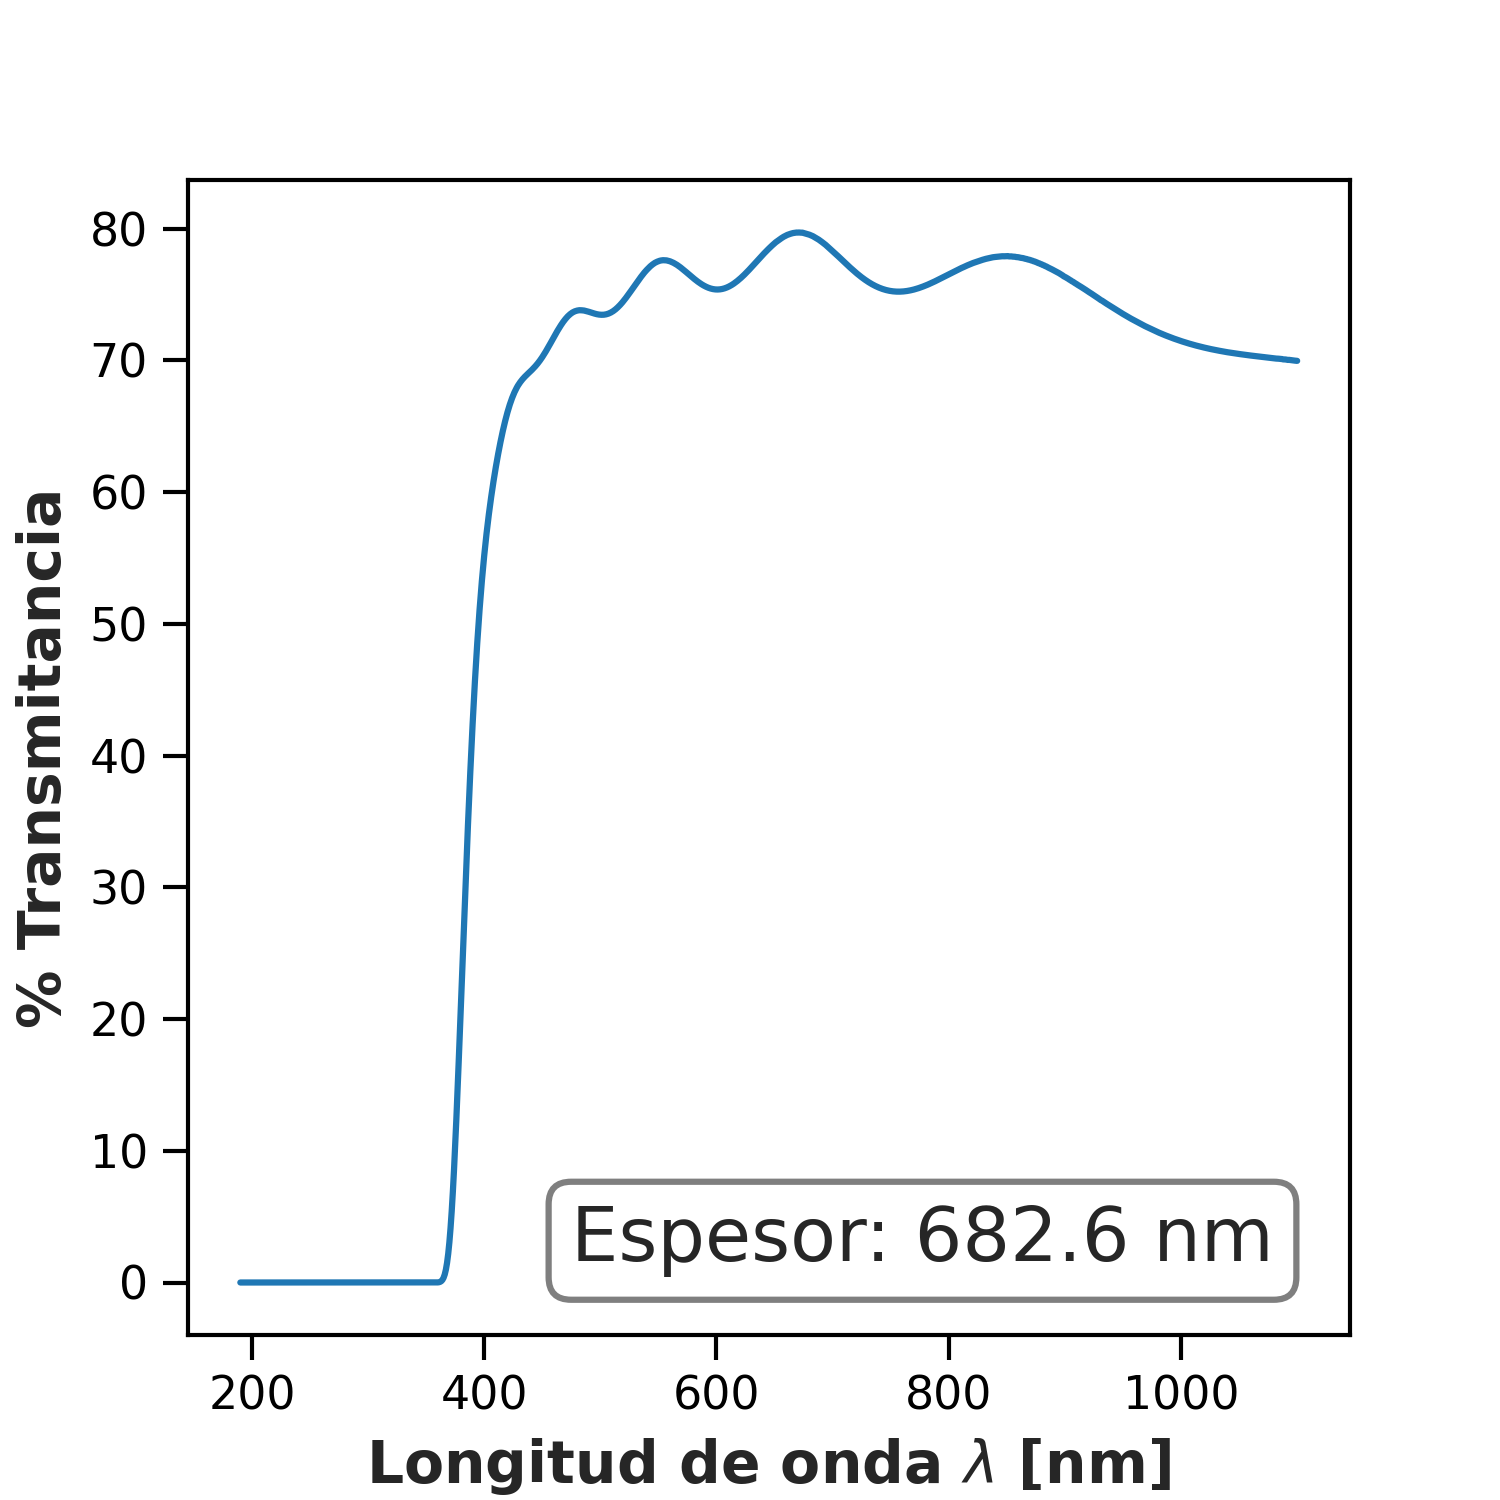
\includegraphics[width=0.48\textwidth]{r3.png}
\caption{Espectros de transmitancia simulados: Regi\'on R$_1$ (izq.) y Regi\'on R$_3$ (der.).}
\label{fig:spec-samples}
\end{figure}

\begin{figure}[htbp]
\centering
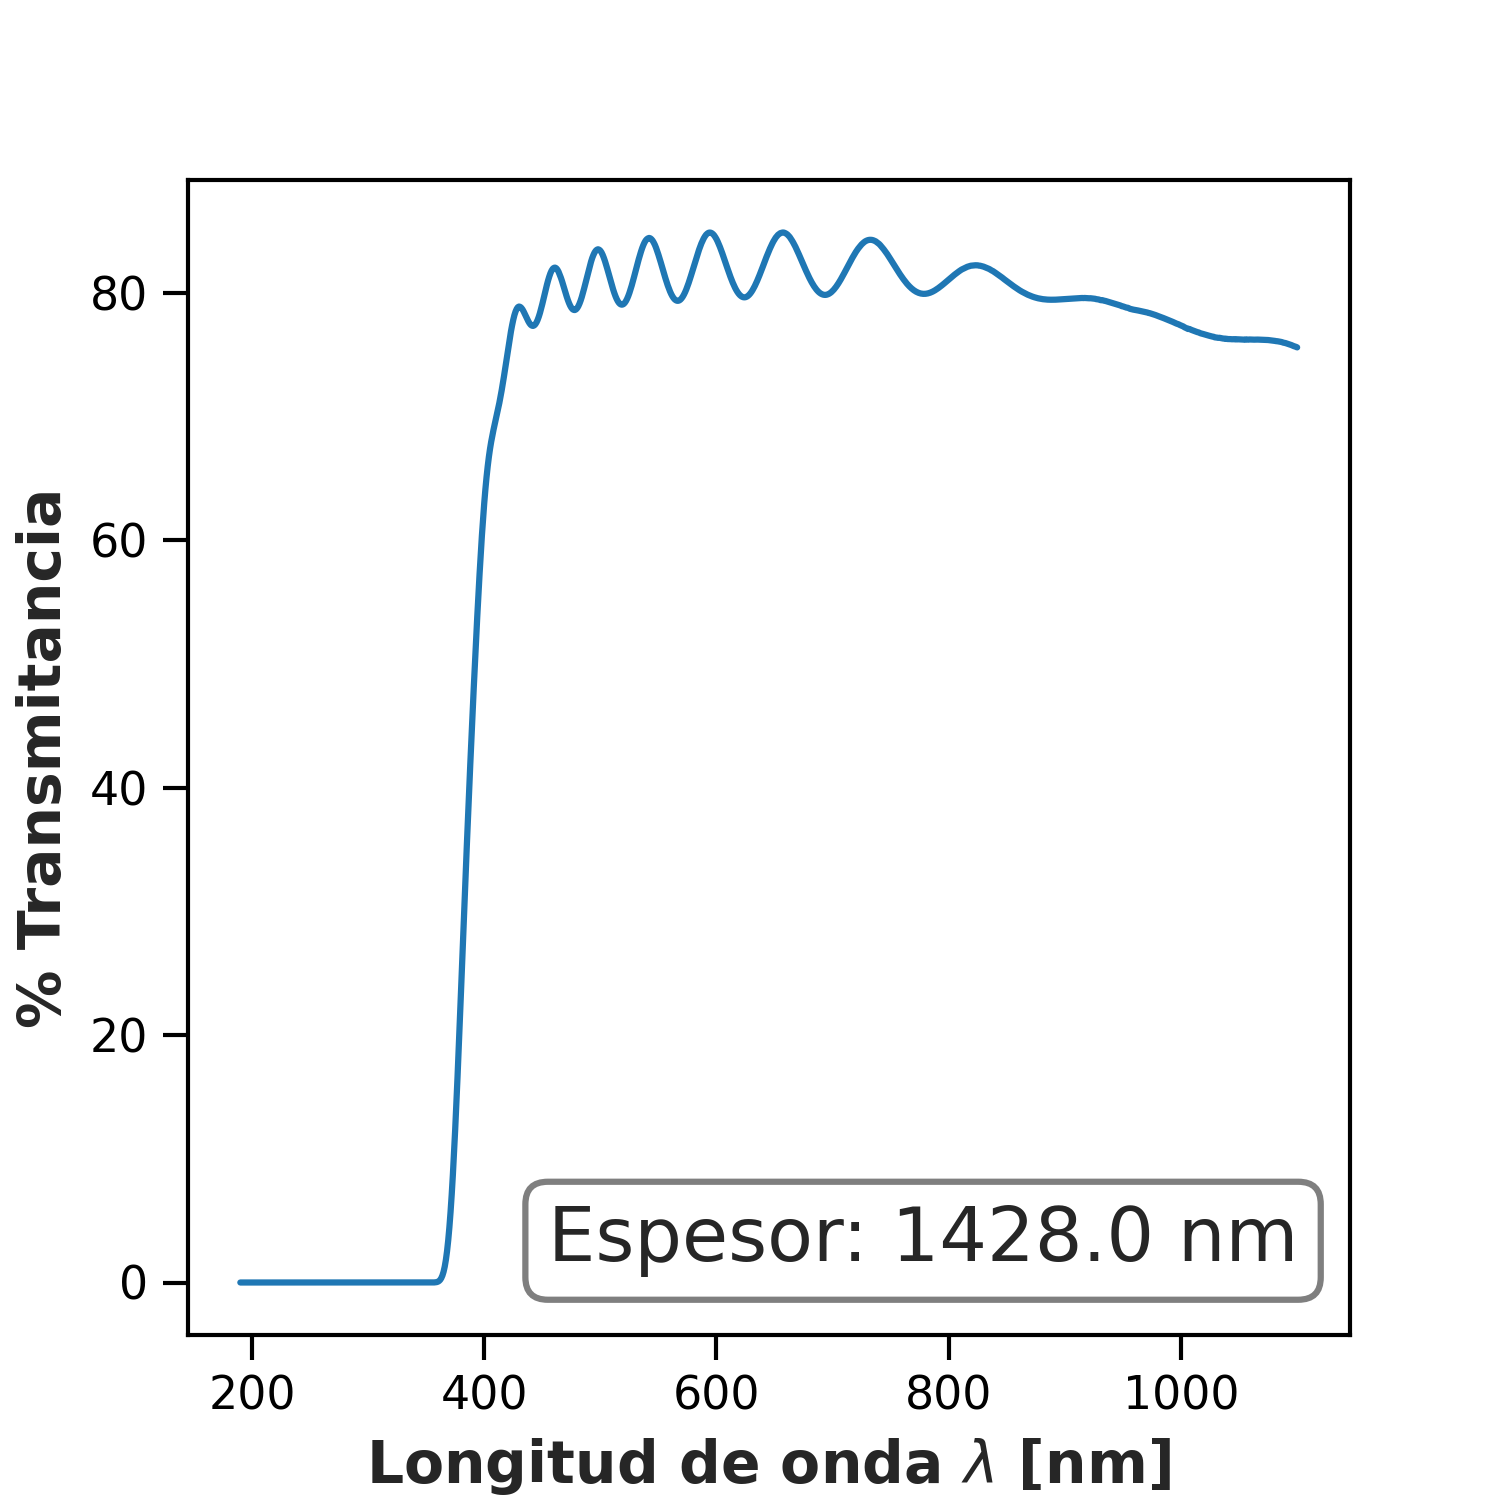
\includegraphics[width=0.7\textwidth]{r5.png}
\caption{Espectro de transmitancia simulado: Regi\'on R$_5$ ($1100$--$1500$ nm).}
\label{fig:spec-r5}
\end{figure}

% Thickness comparison
\begin{figure}[htbp]
\centering
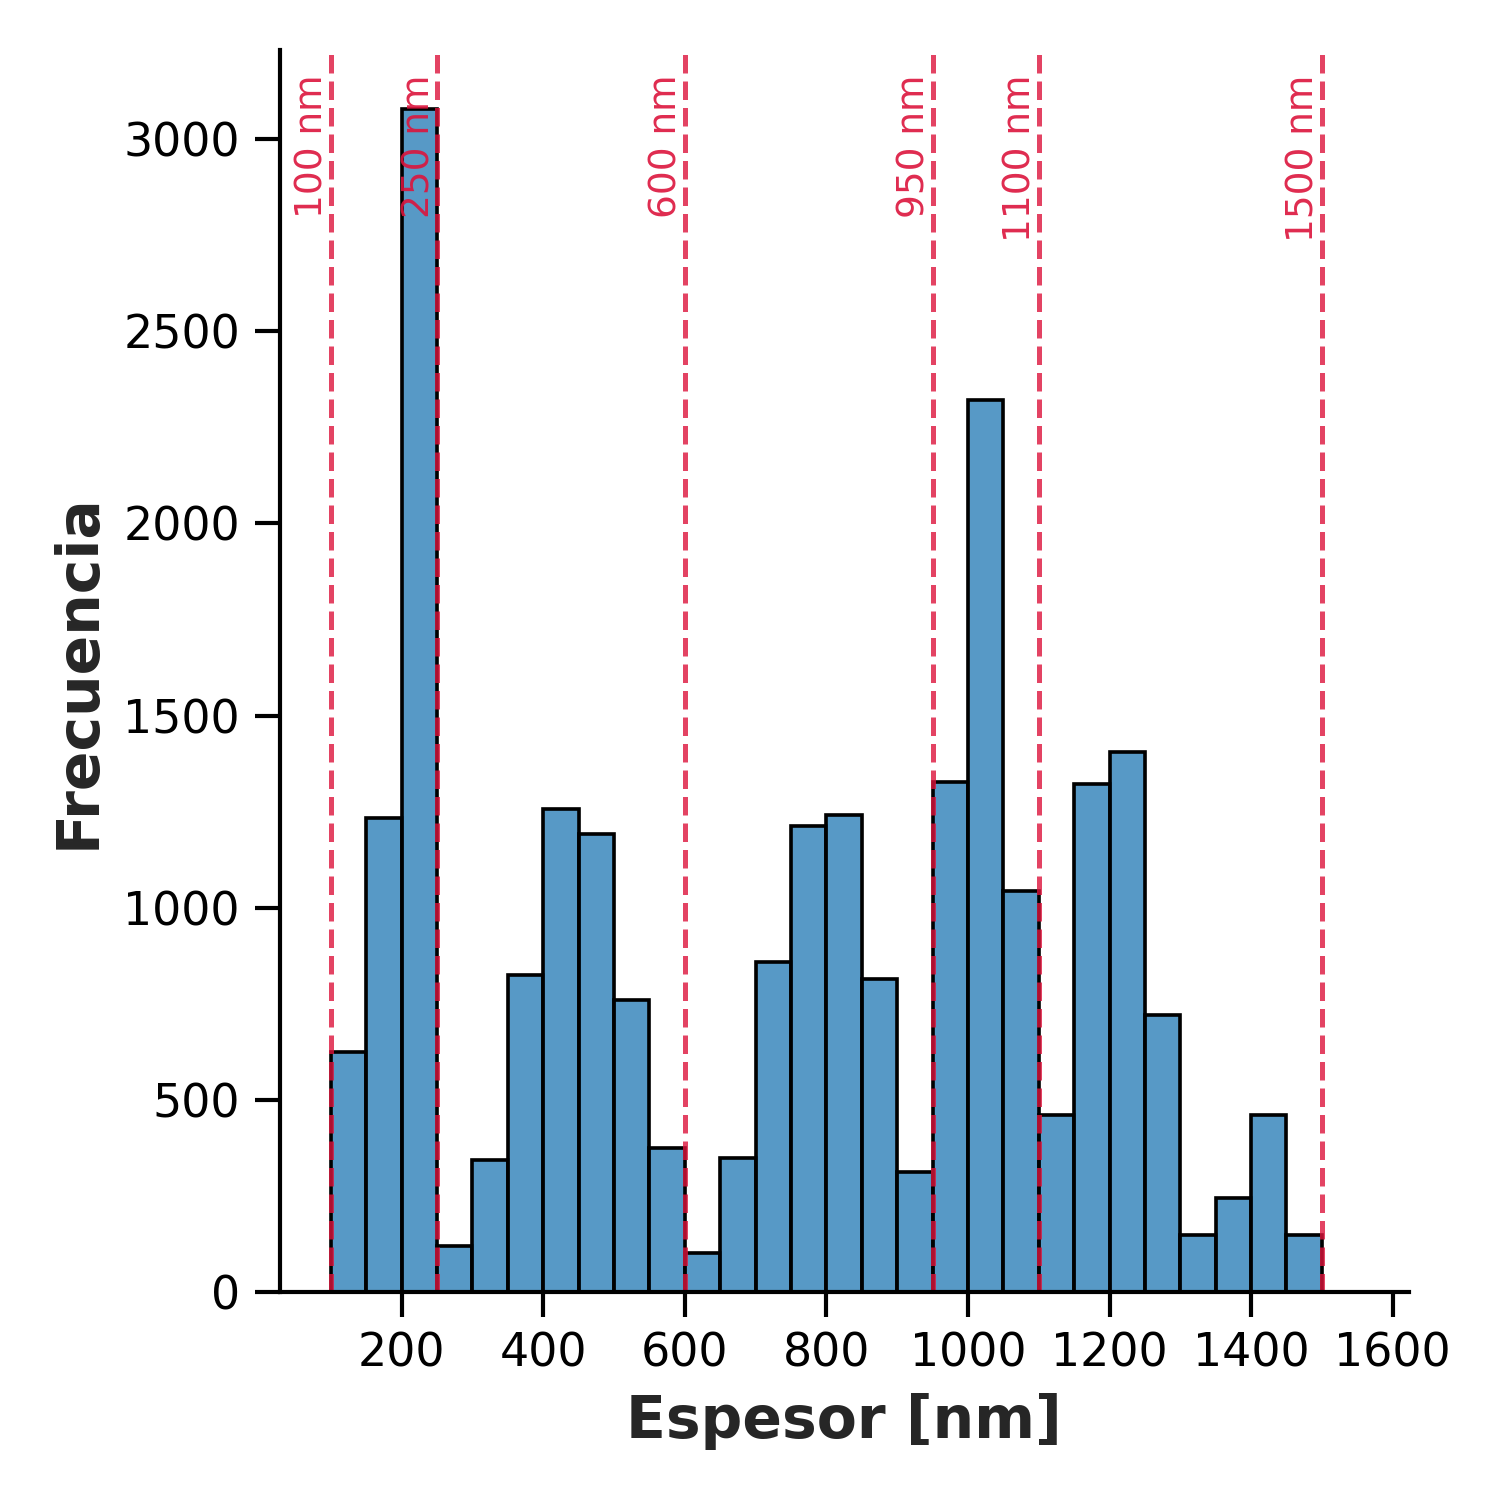
\includegraphics[width=0.7\textwidth]{allthickness.png}
\caption{Histograma de espesores simulados ($\sim$1.2M muestras, bins de 50 nm).}
\label{fig:all-thickness}
\end{figure}

\begin{figure}[htbp]
\centering
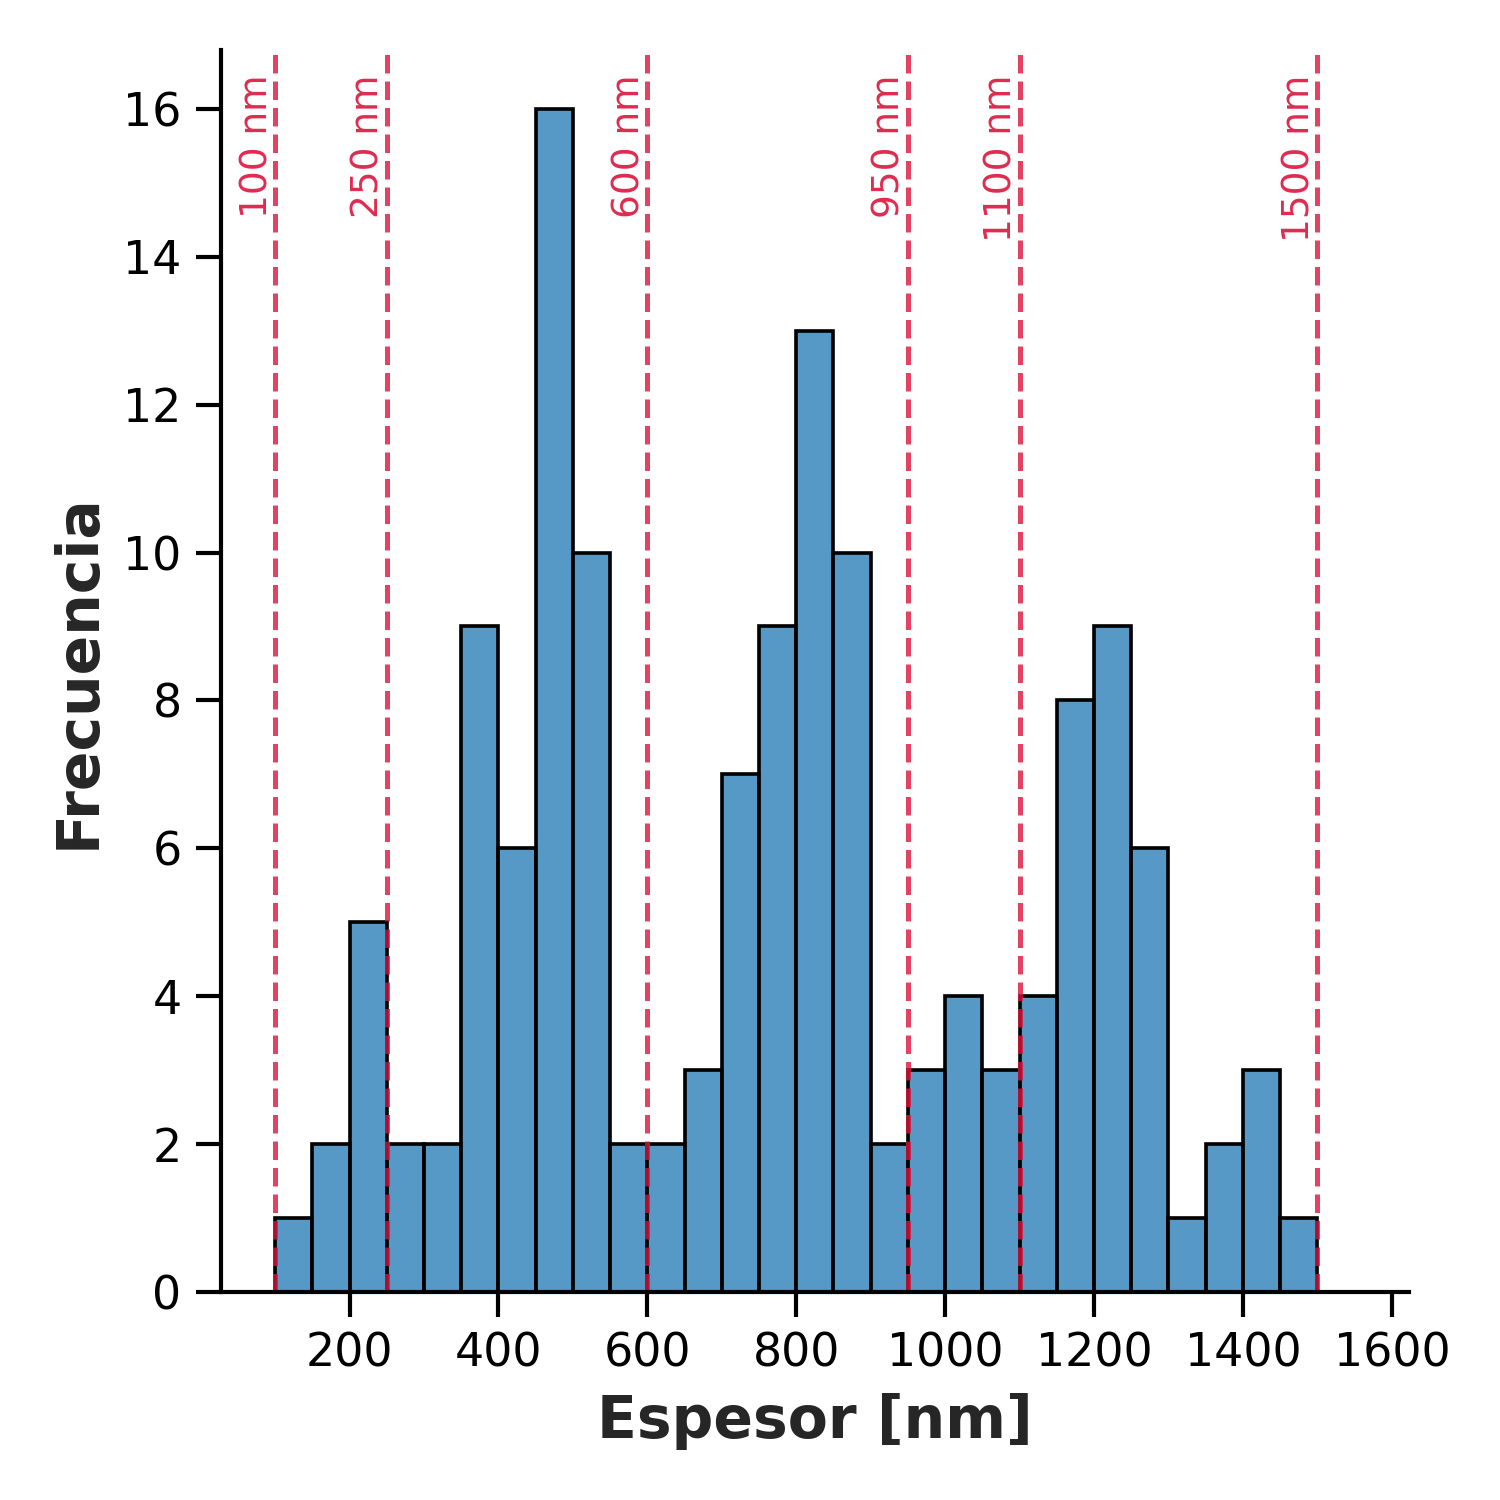
\includegraphics[width=0.7\textwidth]{145thickness.png}
\caption{Histograma de espesores originales (145 muestras experimentales).}
\label{fig:145-thickness}
\end{figure}

\begin{figure}[htbp]
\centering
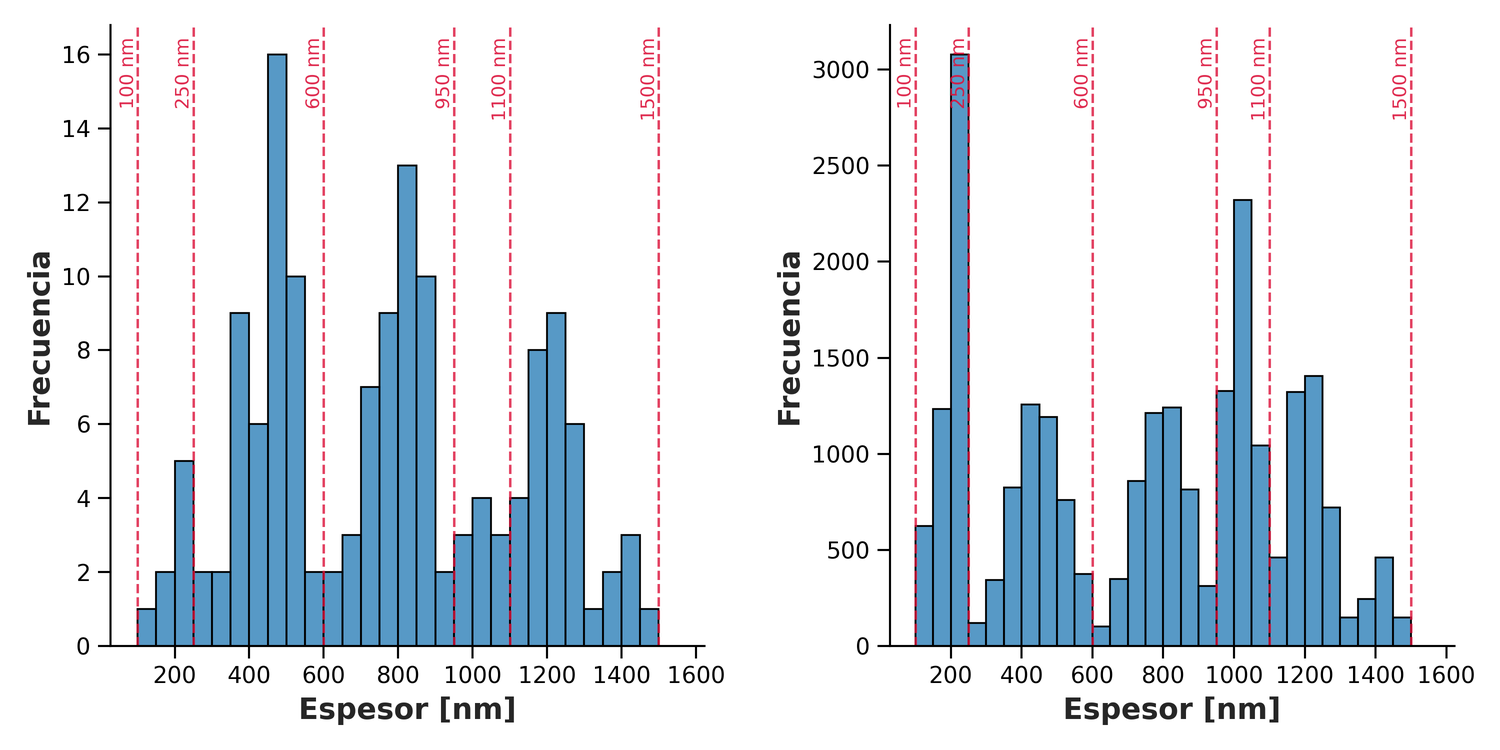
\includegraphics[width=0.85\textwidth]{combined_hist_thickness.png}
\caption{Comparaci\'on de histogramas: simulado vs original.}
\label{fig:hist-comp}
\end{figure}

\begin{figure}[htbp]
\centering
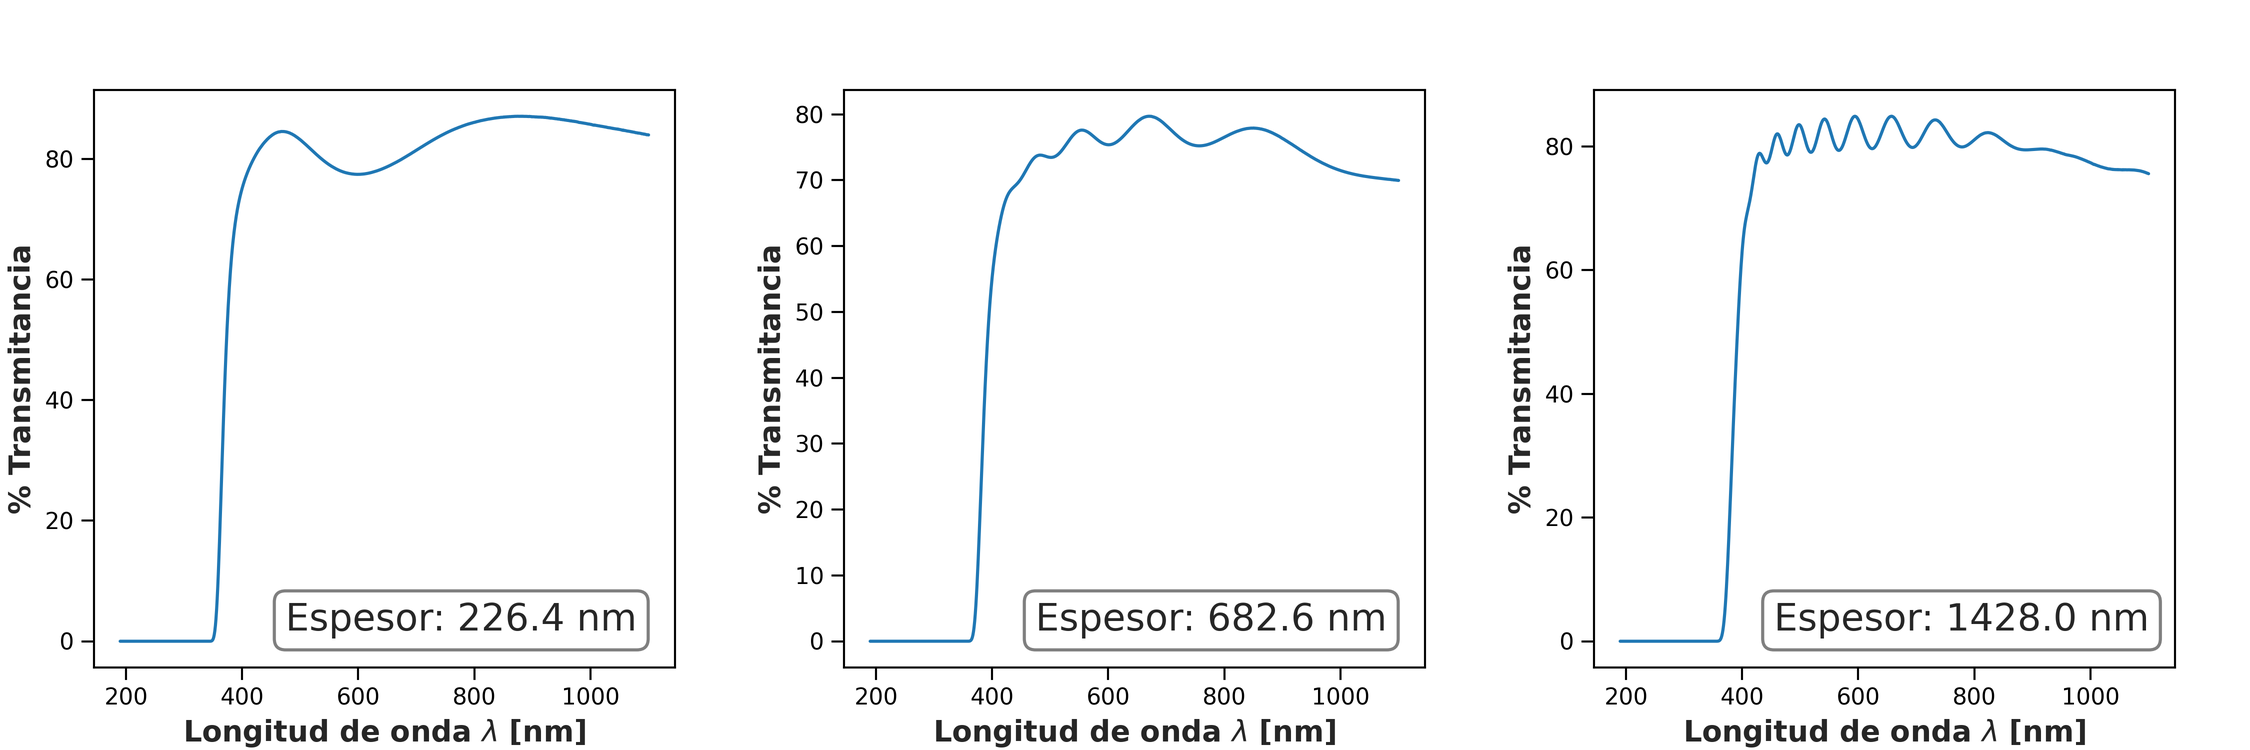
\includegraphics[width=0.85\textwidth]{combined_spectrums.png}
\caption{Composici\'on $1 \times 3$ de espectros simulados de las regiones R$_1$, R$_3$ y R$_5$.}
\label{fig:combined-specs}
\end{figure}

% ============================================================
% ============================================================
% AzONetV2 — Reporte Técnico: Parte 2 (Capítulos 4–7 + Conclusión)
% ============================================================

%%%%%%%%%%%%%%%%%%%%%%%%%%%%%%%%%%%%%%%%%%%%%%%%%%%%%%%%%%%%%%
%% CAPÍTULO 4: BÚSQUEDA DE HIPERPARÁMETROS
%%%%%%%%%%%%%%%%%%%%%%%%%%%%%%%%%%%%%%%%%%%%%%%%%%%%%%%%%%%%%%
\section{Búsqueda de Hiperparámetros para Modelos de Aprendizaje Profundo}
\label{sec:hp-search}

\subsection{Resumen General}

Se presenta una búsqueda sistemática de hiperparámetros para tres arquitecturas de redes neuronales aplicadas a la predicción de espesor de películas delgadas de AZO a partir de espectros de transmitancia sintéticos. La búsqueda utiliza \texttt{keras\_tuner.BayesianOptimization} con las bibliotecas personalizadas \textbf{AmaroX} y \textbf{AmaroXI}. El objetivo es encontrar la arquitectura y el esquema de regularización que minimicen el Error Porcentual Absoluto Medio (MAPE) en un conjunto de validación independiente.

Todos los datos de entrenamiento provienen del pipeline de simulación de datos (Capítulo~3): aproximadamente 1.2 millones de espectros de transmitancia sintéticos (911 puntos, 190--1100~nm) con valores de espesor conocidos.

\subsection{Justificación de U-NET sobre DNN}

Las Redes Neuronales Profundas (DNN) entrenadas sobre espectros de transmitancia aplanados alcanzaron un error mínimo de validación de aproximadamente 10.5\% MAPE. Este error relativamente elevado se atribuye a que un espectro de transmitancia posee una \textbf{estructura espacial intrínseca}: la posición de cada valor de transmitancia en su correspondiente longitud de onda define de manera única la curva espectral.

En contraste, las Redes Neuronales Convolucionales —y particularmente las estructuras tipo autoencoder como U-NET— aplican filtros localizados que se deslizan a lo largo de la entrada, explotando naturalmente las correlaciones espaciales. Entre las variantes convolucionales, las arquitecturas U-NET con capas anidadas han demostrado un rendimiento superior para tareas de regresión sobre señales 1D estructuradas.

\subsection{Configuración Experimental}

\subsubsection{Datos}
\begin{itemize}
\item Origen: Espectros sintéticos del Capítulo~3.
\item Scripts DNN: cargan desde \texttt{data\_simulation/F2} (formato HDF5).
\item Scripts U-NET: cargan desde \texttt{data\_simulation/F1} (formato HDF5).
\item Formato: \texttt{x\_total} (n, 911, 1) \texttt{float32}, normalizado a [0,1]; \texttt{y\_total} (n, 1) \texttt{float32}, espesor en nm.
\item Tamaño del subconjunto: 1/10 del dataset completo — aproximadamente 108,000 entrenamiento / 10,800 prueba / 1,200 validación.
\item Normalización: Min-Max a [0,1] mediante utilidades de AmaroX.
\end{itemize}

\subsubsection{Configuración de Entrenamiento}
\begin{itemize}
\item Tuner: \texttt{keras\_tuner.BayesianOptimization}.
\item Trials: 50 por búsqueda.
\item Ejecuciones por trial: 2.
\item Épocas: 25 (DNN) / 10 (U-NET).
\item Batch size: 512.
\item Loss: MAE (DNN, U-NET Fase 1).
\item Métrica: MAPE.
\item Objetivo: minimizar \texttt{val\_mape}.
\item GPU: GPU única mediante AmaroX \texttt{get\_gpu()}.
\end{itemize}

\subsection{Resultados de Redes Neuronales Profundas (DNN)}

\subsubsection{DNN 5 Capas Ocultas}
Búsqueda de arquitectura: Nodos-$i \in [50, 500]$ paso 50, Dropout $\in [0, 50]$ paso 2, L1/L2 $\in \{10^{-6},\dots,1\}$.

\begin{table}[htbp]
\centering
\caption{Top 5 — DNN 5 Capas Ocultas (de \texttt{best\_models.txt} DNN\_HP\_5).}
\label{tab:dnn5}
\begin{tabular}{cccc}
\hline
\# & Trial & Nodos & MAPE \\
\hline
1 & 43 & [400, 50, 300, 100, 250] & 12.33\% \\
2 & 00 & [300, 400, 500, 450, 350] & 12.63\% \\
3 & 33 & [350, 400, 200, 100, 300] & 12.63\% \\
4 & 39 & [100, 50, 500, 250, 400] & 13.27\% \\
5 & 40 & [400, 400, 350, 100, 200] & 13.85\% \\
\hline
\end{tabular}
\end{table}

\textbf{Mejor: Nodos [400, 50, 300, 100, 250], MAPE = 12.33\%.} La búsqueda de regularizadores (arquitectura fija, Dropout + L1/L2) no mejoró este resultado.

\subsubsection{DNN 7 Capas Ocultas}

\begin{table}[htbp]
\centering
\caption{Top 5 — DNN 7 Capas Ocultas (DNN\_HP\_7).}
\label{tab:dnn7}
\begin{tabular}{cccc}
\hline
\# & Trial & Nodos & MAPE \\
\hline
1 & 27 & [500, 300, 50, 500, 50, 400, 500] & \textbf{10.79\%} \\
2 & 04 & [500, 250, 50, 500, 100, 350, 500] & 10.87\% \\
3 & 26 & [500, 300, 50, 400, 100, 400, 500] & 11.00\% \\
4 & 25 & [500, 250, 100, 500, 100, 450, 500] & 12.21\% \\
5 & 31 & [450, 350, 300, 200, 200, 100, 400] & 12.26\% \\
\hline
\end{tabular}
\end{table}

\textbf{Mejor: Nodos [500, 300, 50, 500, 50, 400, 500], MAPE = 10.79\%} — mejora respecto a 5HL (12.33\%). La regularización no aportó mejoras adicionales.

\subsubsection{DNN 10 Capas Ocultas}

\begin{table}[htbp]
\centering
\caption{Top 5 — DNN 10 Capas Ocultas (DNN\_HP\_10).}
\label{tab:dnn10}
\begin{tabular}{cccc}
\hline
\# & Trial & Nodos & MAPE \\
\hline
1 & 27 & [500, 300, 100, 200, 450, 300, 150, 300, 300, 500] & \textbf{10.51\%} \\
2 & 36 & [500, 250, 50, 300, 100, 200, 200, 50, 350, 250] & 10.85\% \\
3 & 32 & [300, 350, 250, 150, 100, 400, 350, 300, 150, 300] & 11.10\% \\
4 & 39 & [250, 400, 150, 250, 400, 350, 250, 350, 100, 350] & 11.58\% \\
5 & 46 & [350, 450, 150, 100, 50, 450, 350, 150, 400, 400] & 11.78\% \\
\hline
\end{tabular}
\end{table}

\textbf{Mejor: Nodos [500, 300, 100, 200, 450, 300, 150, 300, 300, 500], MAPE = 10.51\%} — mejor resultado DNN en todas las profundidades. La regularización no mejoró este resultado.

\subsubsection{Resumen DNN}

\begin{table}[htbp]
\centering
\caption{Resumen comparativo de arquitecturas DNN.}
\label{tab:dnn-summary}
\begin{tabular}{lcc}
\hline
Arquitectura & Mejor MAPE & Mejor Configuración de Nodos \\
\hline
DNN 5HL  & 12.33\% & [400, 50, 300, 100, 250] \\
DNN 7HL  & 10.79\% & [500, 300, 50, 500, 50, 400, 500] \\
DNN 10HL & \textbf{10.51\%} & [500, 300, 100, 200, 450, 300, 150, 300, 300, 500] \\
\hline
\end{tabular}
\end{table}

Aumentar la profundidad de 5 a 10 capas proporciona una mejora modesta de 12.33\% a 10.51\% MAPE. Sin embargo, el error permanece por encima del 10\%, lo que motiva la exploración de arquitecturas convolucionales.

\subsection{Arquitectura U-NET}

\subsubsection{Componentes Fijos de Diseño}

\textbf{Sección U-NET (Codificador-Decodificador Convolucional):}
\begin{itemize}
\item Número de bloques: 3 (profundidad suficiente para compresión $911 \rightarrow 1$).
\item Filtros base $F$: Buscado (Fase 1), fijado en 21. Se duplica por bloque: $F_i = 2 \cdot F_{i-1}$.
\item Tamaños de kernel: [150, 50, 5]. $K_0 = 150$ elegido de la distancia máx-mín entre franjas para películas de 100--250~nm.
\item Inicializador de pesos: He Normal.
\item Regularizadores L1\_Conv, L2\_Conv: Buscados (Fase 2).
\item Pooling: Average Pooling con \texttt{pool\_size = stride = 4}.
\item Tipo de padding: \texttt{valid}.
\item Activación interna: LeakyReLU.
\end{itemize}

\textbf{Cabezal DNN (Regresión de Espesor):}
Después de que el codificador-decodificador U-NET procesa el espectro, la salida se aplana y se pasa a través de una red Dense de 3 capas:
\begin{itemize}
\item Capas ocultas: 3.
\item Nodos por capa: Buscados (Fase 1), fijados en [470, 340, 330].
\item Dropout: Buscado.
\item Regularizadores L1, L2: Buscados (Fase 2).
\item Activación interna: LeakyReLU, init He Normal.
\item Salida: 1 neurona, ReLU.
\end{itemize}

\subsubsection{Estrategia de Búsqueda en Dos Fases}

\textbf{Fase 1 — Descubrimiento de Arquitectura:} Objetivo: encontrar la mejor combinación de filtros U-NET y nodos del cabezal DNN, sin regularización. Espacio de búsqueda: $F \in [2, 30]$ paso 1, $n_i \in [50, 500)$ paso 10, $D \in [0, 50\%)$ paso 5. 50 trials $\times$ 2 ejecuciones, 10 épocas. Nótese que la Fase 1 optimiza \texttt{val\_accuracy}, no \texttt{val\_mape}.

\begin{table}[htbp]
\centering
\caption{Top 10 — U-NET Fase 1: Descubrimiento de Arquitectura (de \texttt{best\_models\_unet3m.txt}).}
\label{tab:unet-phase1}
\begin{tabular}{cccccc}
\hline
\# & Trial & $F$ & Nodos & Dropout & Accuracy \\
\hline
1 & 187 & \textbf{21} & [470, 340, 330] & 25\% & \textbf{93.82\%} \\
2 & 042 & 25 & [190, 450, 380] & 5\%  & 92.87\% \\
3 & 265 & 19 & [420, 290, 270] & 20\% & 91.85\% \\
4 & 093 & 27 & [130, 150, 180] & 10\% & 91.67\% \\
5 & 211 & 11 & [310, 420, 160] & 40\% & 91.53\% \\
6 & 148 & 21 & [380, 470, 330] & 45\% & 91.38\% \\
7 & 076 & 15 & [290, 320, 440] & 10\% & 90.87\% \\
8 & 299 & 27 & [480, 210, 390] & 30\% & 90.26\% \\
9 & 033 & 13 & [90, 460, 270]  & 35\% & 89.92\% \\
10& 154 & 29 & [70, 380, 490]  & 20\% & 89.66\% \\
\hline
\end{tabular}
\end{table}

\textbf{Mejor: $F=21$, $n=[470,340,330]$, $D=25\%$, accuracy 93.82\% ($\approx 6.18\%$ MAPE).} Todos los 3 mejores candidatos logran MAPE por debajo del 10\%, superando ya al mejor DNN (10.51\%).

\textbf{Fase 2 — Optimización de Regularizadores:} Objetivo: reducir aún más el sobreajuste buscando regularizadores sobre la mejor arquitectura de la Fase 1. Fijo: $F=21$, $n=[470,340,330]$. Espacio de búsqueda: $D \in [0,50)$ paso 5, L1\_Conv, L2\_Conv, L1, L2 $\in \{10^{-6},\dots,1\}$.

\begin{table}[htbp]
\centering
\caption{Top 10 — U-NET Fase 2: Optimización de Regularizadores (de \texttt{DNN\_UNET\_F1\_R/best\_models.txt}).}
\label{tab:unet-phase2}
\begin{tabular}{cccccccc}
\hline
\# & Trial & $D$ & L1 & L2 & L1C & L2C & MAPE \\
\hline
1 & 29 & 35\% & $10^{-6}$ & $10^{-5}$ & $10^{-6}$ & $10^{-4}$ & \textbf{5.77\%} \\
2 & 44 & 30\% & $10^{-6}$ & $10^{-6}$ & $10^{-6}$ & $10^{-6}$ & 6.88\% \\
3 & 20 & 25\% & $10^{-6}$ & $10^{-6}$ & $10^{-4}$ & $10^{-5}$ & 6.99\% \\
4 & 37 & 35\% & $10^{-6}$ & $10^{-5}$ & $10^{-6}$ & $10^{-3}$ & 7.10\% \\
5 & 14 & 25\% & $10^{-6}$ & $10^{-5}$ & $10^{-6}$ & $10^{-4}$ & 7.23\% \\
6 & 41 & 30\% & $10^{-6}$ & $10^{-6}$ & $10^{-6}$ & $10^{-6}$ & 7.64\% \\
7 & 38 & 35\% & $10^{-6}$ & $10^{-5}$ & $10^{-6}$ & $10^{-4}$ & 7.67\% \\
8 & 21 & 35\% & $10^{-6}$ & $10^{-5}$ & $10^{-5}$ & $10^{-4}$ & 7.70\% \\
9 & 28 & 50\% & $10^{-6}$ & $10^{-6}$ & $10^{-6}$ & $10^{-3}$ & 7.84\% \\
10& 18 & 40\% & $10^{-6}$ & $10^{-6}$ & $10^{-4}$ & $10^{-3}$ & 8.15\% \\
\hline
\end{tabular}
\end{table}

\textbf{Mejor: $D=35\%$, L1=$10^{-6}$, L2=$10^{-5}$, L1C=$10^{-6}$, L2C=$10^{-4}$, MAPE = 5.77\%} — mejora adicional respecto a Fase 1 (6.18\%).

\subsubsection{Análisis de Patrones de Regularización}
\begin{itemize}
\item Los regularizadores L1 convergen al valor más pequeño ($10^{-6}$) en casi todos los mejores trials $\rightarrow$ la dispersión L1 no es beneficiosa para este problema.
\item Los regularizadores L2 toman valores en $\{10^{-6}, 10^{-5}, 10^{-4}\}$ $\rightarrow$ un L2 suave previene el sobreajuste sin suprimir características relevantes.
\item El Dropout converge a 30--35\% en los mejores trials, mayor que en Fase 1 (25\%) $\rightarrow$ el L2 adicional permite un dropout más fuerte sin degradar el rendimiento.
\end{itemize}

\subsection{Comparación Final}

\begin{table}[htbp]
\centering
\caption{Comparación final de todos los modelos.}
\label{tab:final-compare}
\begin{tabular}{lccc}
\hline
Modelo & Mejor MAPE & Mejora & Parámetros Clave \\
\hline
DNN 5HL      & 12.33\% & baseline   & Nodos [400,50,300,100,250] \\
DNN 7HL      & 10.79\% & $-1.54$ pp & Nodos [500,300,50,500,50,400,500] \\
DNN 10HL     & 10.51\% & $-1.82$ pp & Nodos [500,300,100,200,450,300,150,300,300,500] \\
U-NET Fase 1 & $\sim$6.18\% & $-4.33$ pp & $F$=21, nodos [470,340,330], $D$=25\% \\
\textbf{U-NET Fase 2} & \textbf{5.77\%} & \textbf{$-4.74$ pp} & $F$=21, nodos [470,340,330], $D$=35\%, L1=$10^{-6}$, L2=$10^{-5}$, L1C=$10^{-6}$, L2C=$10^{-4}$ \\
\hline
\end{tabular}
\end{table}

La arquitectura U-NET \textbf{duplica} el rendimiento en comparación con la mejor DNN (5.77\% vs 10.51\% MAPE), confirmando la hipótesis de que las arquitecturas convolucionales son fundamentalmente más adecuadas para aprender a partir de espectros de transmitancia estructurados.

\subsection{Dependencias}
\texttt{keras}, \texttt{keras\_tuner}, \texttt{AmaroX/AmaroXI}, \texttt{pandas}, \texttt{numpy}, \texttt{h5py}.

\newpage

%%%%%%%%%%%%%%%%%%%%%%%%%%%%%%%%%%%%%%%%%%%%%%%%%%%%%%%%%%%%%%
%% CAPÍTULO 5: ENTRENAMIENTO DE PRODUCCIÓN U-NET CON PÉRDIDA MSE
%%%%%%%%%%%%%%%%%%%%%%%%%%%%%%%%%%%%%%%%%%%%%%%%%%%%%%%%%%%%%%
\section{Entrenamiento de Producción U-NET con Pérdida MSE}
\label{sec:prod-training}

\subsection{Resumen General}

Esta sección describe la ejecución de entrenamiento de producción para la mejor arquitectura U-NET identificada durante la búsqueda de hiperparámetros. A diferencia de la fase de búsqueda de HP —que utilizó 1/10 del dataset, pérdida MAE y 10 épocas— esta ejecución:
\begin{itemize}
\item Utiliza el dataset sintético completo ($\sim$1.2M de muestras).
\item Cambia la pérdida de MAE a MSE, consistente con el ajuste del modelo físico.
\item Entrena durante 100 épocas con la mejor arquitectura de la Fase 2.
\item Guarda el checkpoint del mejor modelo basado en MAPE de validación.
\item Genera gráficos completos de evaluación y logs de TensorBoard.
\end{itemize}

\subsection{Script}
\textbf{Archivo:} \texttt{0\_UNET\_F145F2\_Colab\_Cleaned.py} (también disponible como \texttt{.ipynb}).

Pipeline:
\begin{enumerate}
\item Montar Google Drive.
\item Cargar archivos HDF5 de train, test, validación.
\item Normalización min-max por muestra a [0,1].
\item Asignación de GPU.
\item Definir arquitectura U-NET $\rightarrow$ DNN con los mejores hiperparámetros fijos.
\item Compilar con Adam, pérdida MSE, métricas MAPE+RMSE.
\item Semilla aleatoria = 13.
\item Entrenar 100 épocas, batch 512.
\item Guardar mejor modelo (monitoreando \texttt{val\_mape}) y modelo final.
\item Generar gráficos de MSE, MAPE, RMSE.
\item Evaluar sobre el conjunto de test.
\end{enumerate}

\subsection{Arquitectura del Modelo}

\subsubsection{Entrada}
Shape: (911, 1) — espectro de transmitancia 1D, normalizado a [0,1].

\subsubsection{Sección U-NET (Codificador-Decodificador Convolucional)}

\begin{table}[htbp]
\centering
\caption{Configuración de la sección U-NET.}
\label{tab:unet-config}
\begin{tabular}{lll}
\hline
Parámetro & Valor & Descripción \\
\hline
Filtros base & 21 & Se duplica por bloque: $F_i = 21 \times 2^i$ \\
Kernels & [150, 50, 5] & Tamaños de kernel para 3 bloques del encoder \\
Inicializador & He Normal & Inicializador de pesos \\
Reg. de kernel & L1L2($l_1=10^{-6}$, $l_2=10^{-4}$) & Regularización convolucional \\
Padding & \texttt{valid} & Dimensiones de salida por fórmula \\
Activación & LeakyReLU & Activación interna \\
Pool / stride & 4 / 4 & Average Pooling \\
\hline
\end{tabular}
\end{table}

\textbf{Ruta del Codificador} (3 bloques de downsampling con conexiones de salto):
\begin{itemize}
\item Bloque 0: 21 filtros, kernel 150, entrada (911, 1) $\rightarrow$ salida tras pool (227, 21).
\item Bloque 1: 42 filtros, kernel 50, entrada (227, 21) $\rightarrow$ salida tras pool (56, 42).
\item Bloque 2: 84 filtros, kernel 5, entrada (56, 42) $\rightarrow$ salida tras pool (13, 84).
\end{itemize}

\textbf{Cuello de Botella (Bottleneck):} Sin pooling. 168 filtros, kernel 5. Entrada (13, 84).

\textbf{Ruta del Decodificador} (3 bloques de upsampling con conexiones de salto):
\begin{itemize}
\item Bloque 2 Up: 84 filtros, kernel 5, concatena con salto del encoder bloque 1.
\item Bloque 1 Up: 42 filtros, kernel 50, concatena con salto del encoder bloque 0.
\item Bloque 0 Up: 21 filtros, kernel 150, concatena con la entrada original.
\end{itemize}

\textbf{Convolución Final:} Conv1D(1, kernel=1, LeakyReLU) $\rightarrow$ salida (911, 1).

\subsubsection{Cabezal DNN (Regresión de Espesor)}
Después de aplanar la salida U-NET, se pasa a través de una red Dense de 3 capas:

\begin{table}[htbp]
\centering
\caption{Configuración del cabezal DNN.}
\label{tab:dnn-head}
\begin{tabular}{ll}
\hline
Parámetro & Valor \\
\hline
Nodos & [470, 340, 330] \\
Dropout & 35\% \\
L1 & $10^{-6}$ \\
L2 & $10^{-5}$ \\
Activación interna & LeakyReLU \\
Inicializador & He Normal \\
Salida & 1 neurona, ReLU \\
\hline
\end{tabular}
\end{table}

Cada capa Dense es seguida por Dropout y BatchNormalization.

\subsubsection{Diagrama de Arquitectura}

\begin{figure}[htbp]
\centering

\includegraphics[width=0.55\textwidth]{model.png}
\caption{Diagrama de arquitectura del modelo U-NET + DNN.}
\label{fig:model-arch}
\end{figure}

\subsection{Pipeline de Datos}

\subsubsection{Normalización por Muestra}
Cada espectro se normaliza independientemente a [0,1] usando su propio mínimo y máximo:
\[
x_{\text{norm}} = \frac{x - \min(x)}{\max(x) - \min(x) + 10^{-6}}
\]

\subsubsection{Carga de Datos HDF5}
Desde \texttt{notebooks/3\_data\_simulation/NewDataAzONetV2/Sets/}:
\begin{itemize}
\item \texttt{train.h5}: $\sim$960,000 muestras (80\%).
\item \texttt{test.h5}: $\sim$120,000 muestras (10\%).
\item \texttt{val.h5}: $\sim$120,000 muestras (10\%).
\end{itemize}

\subsection{Configuración de Entrenamiento}

\begin{table}[htbp]
\centering
\caption{Configuración de entrenamiento de producción.}
\label{tab:train-config}
\begin{tabular}{ll}
\hline
Parámetro & Valor \\
\hline
Pérdida & MSE: $L = \frac{1}{N} \sum (y_{\text{pred}} - y_{\text{true}})^2$ \\
Métricas & MAPE, RMSE \\
Optimizador & Adam ($lr=0.001$) \\
Batch size & 512 \\
Épocas & 100 \\
Semilla & 13 \\
Callbacks & EarlyStopping(patience=1000), ReduceLROnPlateau, \\
 & Checkpoint(val\_mape), CSVLogger, TensorBoard \\
\hline
\end{tabular}
\end{table}

\subsubsection{¿Por qué MSE en lugar de MAE?}
En la búsqueda de HP, los modelos se entrenaron con pérdida MAE. En esta ejecución de producción, la pérdida se cambia a MSE por consistencia con el resto del pipeline:
\begin{itemize}
\item El ajuste DE minimiza MSE entre el modelo y los espectros experimentales.
\item La simulación de datos genera espectros a partir de parámetros optimizados con MSE.
\item Entrenar con el mismo objetivo (MSE) alinea la señal de aprendizaje con el proceso de generación de datos.
\end{itemize}

\subsection{Resultados de Entrenamiento}

\subsubsection{Mejor Modelo (Época 39)}
El mejor rendimiento de validación (menor \texttt{val\_mape}) se alcanzó en la época 39:

\begin{table}[htbp]
\centering
\caption{Métricas del mejor modelo (Época 39).}
\label{tab:best-model}
\begin{tabular}{lcc}
\hline
Métrica & Entrenamiento & Validación \\
\hline
MSE (nm$^2$) & 699.75 & \textbf{18.28} \\
MAPE (\%)    & 4.76\% & \textbf{0.61\%} \\
RMSE (nm)    & 26.39  & \textbf{3.85} \\
\hline
\end{tabular}
\end{table}

\subsubsection{Modelo Final (Época 99)}
Después de 100 épocas, el modelo había sobreajustado significativamente:

\begin{table}[htbp]
\centering
\caption{Métricas del modelo final (Época 99).}
\label{tab:final-model}
\begin{tabular}{lcc}
\hline
Métrica & Entrenamiento & Validación \\
\hline
MSE (nm$^2$) & 660.20 & 260.79 \\
MAPE (\%)    & 4.60\% & 2.20\% \\
RMSE (nm)    & 25.58  & 15.96 \\
\hline
\end{tabular}
\end{table}

\subsubsection{Dinámica de Entrenamiento}

\begin{table}[htbp]
\centering
\caption{Métricas época por época (épocas seleccionadas).}
\label{tab:epoch-detail}
\begin{tabular}{ccccccc}
\hline
Época & Train MSE & Train MAPE & Train RMSE & Val MSE & Val MAPE & Val RMSE \\
\hline
0  & 178,780 & 48.70\% & 422.8 & 20,029 & 20.62\% & 141.5 \\
1  & 2,718   & 9.95\%  & 52.1  & 862    & 6.51\%  & 29.4 \\
2  & 1,553   & 8.06\%  & 39.4  & 457    & 4.10\%  & 21.4 \\
12 & 799     & 5.18\%  & 28.2  & 1,634  & 4.52\%  & 40.4 \\
22 & 731     & 4.92\%  & 27.0  & 35.3   & 0.88\%  & 5.8 \\
\textbf{39} & \textbf{700} & \textbf{4.76\%} & \textbf{26.4} & \textbf{18.3} & \textbf{0.61\%} & \textbf{3.9} \\
50 & 689     & 4.69\%  & 26.2  & 23.3   & 0.79\%  & 4.4 \\
70 & 673     & 4.63\%  & 25.8  & 484    & 2.08\%  & 21.9 \\
80 & 669     & 4.62\%  & 25.7  & 1,784  & 4.11\%  & 42.2 \\
99 & 660     & 4.60\%  & 25.6  & 261    & 2.20\%  & 16.0 \\
\hline
\end{tabular}
\end{table}

Observaciones:
\begin{enumerate}
\item \textbf{Aprendizaje inicial rápido:} el MSE de la primera época cae de 178,780 a 2,718 (dos órdenes de magnitud).
\item \textbf{Inicio de sobreajuste:} después de la época $\sim$50, las métricas de entrenamiento continúan mejorando mientras que las de validación oscilan hacia arriba.
\item \textbf{Inestabilidad en validación:} alta varianza entre épocas debido al gran batch size o a patrones espectrales poco frecuentes.
\item \textbf{Mejor época (39):} equilibrio óptimo entre subajuste y sobreajuste, val MAPE 0.61\%, val RMSE 3.85~nm.
\end{enumerate}

\subsubsection{Curvas de Entrenamiento}

\begin{figure}[htbp]
\centering

\includegraphics[width=0.48\textwidth]{mae.png}

\includegraphics[width=0.48\textwidth]{mape.png}
\caption{Curvas de entrenamiento: MSE (izq.) y MAPE (der.) sobre 100 épocas.}
\label{fig:training-curves1}
\end{figure}

\begin{figure}[htbp]
\centering

\includegraphics[width=0.7\textwidth]{rmse.png}
\caption{Curva de entrenamiento: RMSE sobre 100 épocas.}
\label{fig:training-curves2}
\end{figure}

\subsection{Comparación: Primera Versión (Pérdida MAE)}

Antes de la ejecución de producción con MSE, se realizó un entrenamiento inicial utilizando pérdida MAE —la misma pérdida usada durante la búsqueda de HP—. Configuración: pérdida MAE, arquitectura idéntica ($F$=21, kernels [150,50,5], nodos [470,340,330], $D$=35\%, L1/L2=$10^{-6}$/$10^{-5}$, L1C/L2C=$10^{-6}$/$10^{-4}$), 100 épocas, batch 512, semilla 13, Adam.

\begin{table}[htbp]
\centering
\caption{Primera versión (MAE) — épocas seleccionadas.}
\label{tab:mae-version}
\begin{tabular}{ccccccc}
\hline
Época & Train MAE & Train MAPE & Train RMSE & Val MAE & Val MAPE & Val RMSE \\
\hline
0  & 226.3 & 33.20\% & 407.7 & 14.0 & 4.58\% & 28.9 \\
1  & 31.9  & 9.19\%  & 45.0  & 19.1 & 7.13\% & 34.8 \\
14 & 22.3  & 5.87\%  & 28.4  & 7.2  & 1.79\% & 8.5 \\
\textbf{17} & \textbf{21.9} & \textbf{5.79\%} & \textbf{28.0} & \textbf{5.8} & \textbf{1.13\%} & \textbf{7.1} \\
50 & 21.3  & 5.70\%  & 27.7  & 6.0  & 1.28\% & 7.7 \\
80 & 20.9  & 5.57\%  & 27.1  & 46.9 & 6.38\% & 64.6 \\
99 & 21.2  & 5.65\%  & 27.5  & 18.3 & 3.99\% & 32.4 \\
\hline
\end{tabular}
\end{table}

Mejor rendimiento: Época 17 con \texttt{val\_mape} = 1.13\%, \texttt{val\_mae} = 5.76~nm, \texttt{val\_rmse} = 7.13~nm.

\subsection{Comparación Directa MAE vs MSE}

\begin{table}[htbp]
\centering
\caption{Comparación directa entre versiones MAE y MSE.}
\label{tab:mae-vs-mse}
\begin{tabular}{lcc}
\hline
Métrica & Primera Versión (MAE) & Producción (MSE) \\
\hline
Función de pérdida & $|y - \hat{y}|$ & $(y - \hat{y})^2$ \\
Mejor época   & 17 & 39 \\
Mejor Val MAPE  & 1.13\% & \textbf{0.61\%} \\
Mejor Val RMSE  & 7.13~nm & \textbf{3.85~nm} \\
Velocidad de convergencia & Más rápida (época 17) & Más lenta (época 39) \\
Inicio de sobreajuste & $\sim$época 20 & $\sim$época 50 \\
\hline
\end{tabular}
\end{table}

El cambio de MAE a MSE produce una mejora relativa del 46\% en MAPE (1.13\% $\rightarrow$ 0.61\%) y del 46\% en RMSE (7.13 $\rightarrow$ 3.85~nm).

Análisis:
\begin{enumerate}
\item \textbf{Penalización cuadrática:} MSE sobre-pondera los errores grandes ($\propto \varepsilon^2$), forzando al optimizador a enfocarse en espectros atípicos.
\item \textbf{Magnitud del gradiente:} MAE tiene gradiente constante ($\pm 1$), el gradiente de MSE escala con el error ($2\varepsilon$) $\rightarrow$ convergencia más fina cerca del óptimo.
\item \textbf{Consistencia con el pipeline:} tanto el ajuste DE como la simulación de datos minimizan MSE, alineando la señal de aprendizaje en todas las etapas.
\end{enumerate}

\subsection{Conclusión del Entrenamiento}

La arquitectura U-NET con hiperparámetros óptimos ($F$=21, nodos [470,340,330], L1C=$10^{-6}$, L2C=$10^{-4}$, L1=$10^{-6}$, L2=$10^{-5}$, $D$=35\%), al entrenarse sobre el dataset sintético completo de 1.2M de muestras con pérdida MSE, alcanza:
\begin{itemize}
\item \textbf{MAPE de validación: 0.61\%} — error promedio de predicción por debajo del 1\%.
\item \textbf{RMSE de validación: 3.85~nm} — RMSE por debajo de 4~nm.
\end{itemize}
Estos resultados validan la estrategia de búsqueda de HP en dos fases y demuestran que las arquitecturas convolucionales pueden aprender efectivamente el mapeo inverso desde espectros de transmitancia hasta el espesor de película.

\subsection{Dependencias}
\texttt{tensorflow 2.x}, \texttt{keras}, \texttt{h5py}, \texttt{numpy}, \texttt{pandas}, \texttt{matplotlib}, \texttt{seaborn}, \texttt{google.colab}, \texttt{AmaroXI}.

\newpage

%%%%%%%%%%%%%%%%%%%%%%%%%%%%%%%%%%%%%%%%%%%%%%%%%%%%%%%%%%%%%%
%% CAPÍTULO 6: PIPELINE DE INFERENCIA Y PREDICCIÓN
%%%%%%%%%%%%%%%%%%%%%%%%%%%%%%%%%%%%%%%%%%%%%%%%%%%%%%%%%%%%%%
\section{Pipeline de Inferencia y Predicción}
\label{sec:inference}

\subsection{Resumen General}

Este capítulo describe el pipeline de inferencia implementado en \texttt{notebooks/6\_results\_colab/Predictions.py}, el cual carga un modelo UNET pre-entrenado para predecir espesores de películas delgadas a partir de datos espectrales tanto simulados como experimentales. Se generan predicciones para las divisiones completas de entrenamiento, prueba y validación, así como para las 145 muestras experimentales externas, exportando todos los resultados como arreglos NumPy.

\subsection{Datos}

\subsubsection{Datasets Simulados}
Las divisiones de entrenamiento, prueba y validación se almacenan como archivos HDF5 bajo \texttt{notebooks/3\_data\_simulation/NewDataAzONetV2/Sets/}. Cada archivo \texttt{.h5} contiene \texttt{x\_total} (espectros de transmitancia) y \texttt{y\_total} (etiquetas de espesor).

\subsubsection{Datos Experimentales}
Los espectros experimentales de las 145 muestras de película delgada se cargan desde \texttt{results/dataframe\_spectrum\_thickness\_145\_final.pkl}. Los valores de espesor de referencia (ground truth) provienen de los parámetros de Evolución Diferencial almacenados en \texttt{results/SciPy\_IIM/differential\_evolution\_NonLinear\_145F.npy}.

\subsection{Metodología}

\subsubsection{Normalización por Muestra}
La normalización se aplica a cada espectro de forma independiente:
\[
x_{\text{norm}} = \frac{x - \min(x)}{\max(x) - \min(x) + 1 \times 10^{-6}}
\]
Esto garantiza que cada espectro quede normalizado al intervalo $[0, 1]$ sin fuga de información entre muestras. El término $10^{-6}$ previene la división por cero en espectros constantes.

\subsubsection{Modelo UNET}
El modelo UNET pre-entrenado se carga desde \texttt{Copia de model.keras}. Se realiza una verificación de integridad evaluando el modelo sobre el conjunto de prueba mediante \texttt{modelo\_UNET.evaluate}, confirmando que los pesos se cargaron correctamente y que las predicciones son coherentes con el rendimiento esperado.

\subsubsection{Asignación de GPU}
Los recursos de GPU se configuran mediante \texttt{tf.config.set\_visible\_devices} de TensorFlow, apuntando al primer dispositivo GPU disponible. Esto es esencial para el entorno de ejecución de Google Colab, garantizando que el modelo utilice la aceleración por hardware durante la inferencia.

\subsection{Predicciones y Salidas}

Las predicciones se generan usando \texttt{modelo\_UNET.predict} para los cuatro subconjuntos de datos:
\begin{itemize}
\item Entrenamiento (Train): predicciones sobre la división de entrenamiento completa ($\sim$960,000 muestras).
\item Prueba (Test): predicciones sobre la división de prueba ($\sim$120,000 muestras).
\item Validación (Validation): predicciones sobre la división de validación ($\sim$120,000 muestras).
\item Experimental 145: predicciones sobre los espectros experimentales externos (145 muestras).
\end{itemize}

Los archivos de salida se guardan en el directorio \texttt{MSE\_data/}:

\begin{table}[htbp]
\centering
\caption{Archivos de salida del pipeline de inferencia.}
\label{tab:inference-outputs}
\begin{tabular}{ll}
\hline
Archivo & Descripción \\
\hline
\texttt{preds\_train.npy} & Predicciones de espesor para el conjunto de entrenamiento \\
\texttt{y\_train.npy}    & Valores reales (ground truth) de entrenamiento \\
\texttt{preds\_test.npy}  & Predicciones de espesor para el conjunto de prueba \\
\texttt{y\_test.npy}      & Valores reales (ground truth) de prueba \\
\texttt{preds\_val.npy}   & Predicciones de espesor para el conjunto de validación \\
\texttt{y\_val.npy}       & Valores reales (ground truth) de validación \\
\texttt{preds\_145.npy}   & Predicciones de espesor para las 145 muestras experimentales \\
\texttt{y\_145.npy}       & Valores reales (ground truth) experimentales (DE) \\
\hline
\end{tabular}
\end{table}

\subsection{Reproducibilidad}
\begin{itemize}
\item Entorno: Google Colab con runtime de GPU.
\item Modelo: \texttt{Copia de model.keras} (UNET pre-entrenado).
\item Script de inferencia: \texttt{notebooks/6\_results\_colab/Predictions.py}.
\item No se utiliza semilla aleatoria explícita; los resultados son deterministas dados los mismos pesos del modelo y los mismos datos de entrada.
\end{itemize}

\newpage

%%%%%%%%%%%%%%%%%%%%%%%%%%%%%%%%%%%%%%%%%%%%%%%%%%%%%%%%%%%%%%
%% CAPÍTULO 7: INFERENCIA FINAL Y EVALUACIÓN ESTADÍSTICA
%%%%%%%%%%%%%%%%%%%%%%%%%%%%%%%%%%%%%%%%%%%%%%%%%%%%%%%%%%%%%%
\section{Inferencia Final y Evaluación Estadística}
\label{sec:final-eval}

\subsection{Resumen General}

Este capítulo presenta una evaluación exhaustiva del modelo UNET de predicción de espesor. Se generaron predicciones para tres divisiones de datos simulados (960,000 entrenamiento, 120,000 validación, 120,000 prueba) y un conjunto de datos experimental externo (145 muestras de película delgada). Se reportan métricas de error (MAE, MSE, RMSE, MAPE, $R^2$) y análisis detallados de las distribuciones del Error Porcentual Absoluto (APE) y del Error Porcentual (PE) para cada división. El modelo alcanza un rendimiento excepcional en datos simulados (MAPE $\approx$ 0.61\%, $R^2 = 0.9999$) con métricas casi idénticas entre divisiones, lo que indica una excelente generalización. En las muestras experimentales, el modelo obtiene un MAPE de 7.38\% y $R^2 = 0.9385$. Notablemente, la distribución del PE en los datos experimentales es normal (Shapiro-Wilk $p = 0.816$).

\subsection{Pipeline de Evaluación}
El pipeline de inferencia consta de dos scripts principales:
\begin{itemize}
\item \texttt{1\_figures\_MSE.py} — Carga las predicciones pre-calculadas (archivos \texttt{.npy} generados en el Capítulo~6), calcula métricas de error y análisis de distribuciones, y genera figuras con calidad de publicación.
\item \texttt{training\_plots.py} — Lee \texttt{training.log} y grafica la evolución de MSE, MAPE y RMSE a lo largo de 100 épocas de entrenamiento.
\end{itemize}

\subsection{Historial de Entrenamiento}
El modelo UNET fue entrenado durante \textbf{100 épocas} utilizando el optimizador \textbf{Adam} con una tasa de aprendizaje $lr = 0.001$. Las métricas finales en la época 100 son:

\begin{table}[htbp]
\centering
\caption{Métricas al final del entrenamiento (Época 100).}
\label{tab:train-final}
\begin{tabular}{lccc}
\hline
Conjunto & MSE (nm$^2$) & MAPE (\%) & RMSE (nm) \\
\hline
Entrenamiento & 660.20 & 4.60\% & 25.58 \\
Validación    & 260.79 & 2.20\% & 15.96 \\
\hline
\end{tabular}
\end{table}

Nota: Las métricas de entrenamiento reportadas aquí representan el error durante la fase de aprendizaje y no deben confundirse con las métricas de inferencia final presentadas en las secciones siguientes, las cuales se calculan sobre el modelo ya entrenado.

%%%%%%%%%%%%%%%%%%%%%%%%%%%%%%%%%%%%%%%%%%%%%%%%%%%%%%%%%%%%%%
\subsection{División Train ($N = 960{,}000$)}
%%%%%%%%%%%%%%%%%%%%%%%%%%%%%%%%%%%%%%%%%%%%%%%%%%%%%%%%%%%%%%

\subsubsection{Métricas de Error}

\begin{table}[htbp]
\centering
\caption{Métricas de error — División Train.}
\label{tab:train-metrics}
\begin{tabular}{ll}
\hline
Métrica & Valor \\
\hline
MAE  & 2.91~nm \\
MSE  & 14.73~nm$^2$ \\
RMSE & 3.84~nm \\
MAPE & 0.61\% \\
$R^2$ & 0.9999 \\
\hline
\end{tabular}
\end{table}

\subsubsection{Distribución APE (Error Porcentual Absoluto)}

\begin{table}[htbp]
\centering
\caption{Estadísticos de la distribución APE — Train.}
\label{tab:train-ape}
\begin{tabular}{ll}
\hline
Estadístico & Valor \\
\hline
Media                    & 0.6120\% \\
Mediana                  & 0.3273\% \\
Desviación Estándar      & 0.8593\% \\
Mínimo                   & 0.00\% \\
Máximo                   & 40.17\% \\
IQR                      & 0.5931\% \\
Asimetría (Skewness)     & 6.2475 (altamente sesgada, derecha/positiva) \\
Curtosis (Exceso)        & 105.3445 (leptocúrtica, colas pesadas) \\
Outliers (IQR)           & 81,990 (8.54\%) \\
Entropía                 & 7.0395 bits \\
Coeficiente de Variación & 1.4040 \\
\hline
\end{tabular}
\end{table}

\textbf{Pruebas de Normalidad — TODAS RECHAZADAS:}
\begin{itemize}
\item Kolmogorov-Smirnov: $D = 0.2382$, $p \approx 0$.
\item Anderson-Darling: $A^2 = 90{,}671.85 > 0.7870$ (rechaza al 5\%).
\item Jarque-Bera: $\text{JB} = 4.50 \times 10^8$, $p \approx 0$.
\end{itemize}

\subsubsection{Distribución PE (Error Porcentual)}

\begin{table}[htbp]
\centering
\caption{Estadísticos de la distribución PE — Train.}
\label{tab:train-pe}
\begin{tabular}{ll}
\hline
Estadístico & Valor \\
\hline
Media                    & $-0.3221\%$ \\
Mediana                  & $-0.0481\%$ \\
Desviación Estándar      & 1.0047\% \\
Asimetría (Skewness)     & $-3.6440$ (altamente sesgada, izquierda/negativa) \\
Curtosis (Exceso)        & 60.9873 (leptocúrtica) \\
Outliers (IQR)           & 62,782 (6.54\%) \\
\hline
\end{tabular}
\end{table}

\textbf{Normalidad:} Rechazada por todas las pruebas (KS $D = 0.1555$, AD $A^2 = 49{,}907.91$, JB $= 1.51 \times 10^8$, todos $p \approx 0$).

La media negativa del PE ($-0.32\%$) indica una tendencia negligible a \textbf{sobre-predecir} ligeramente el espesor. Sin embargo, la mediana ($-0.05\%$) está muy cercana a cero, lo que confirma que el grueso de las predicciones está bien centrado.

\subsubsection{Figuras — División Train}

\begin{figure}[htbp]
\centering
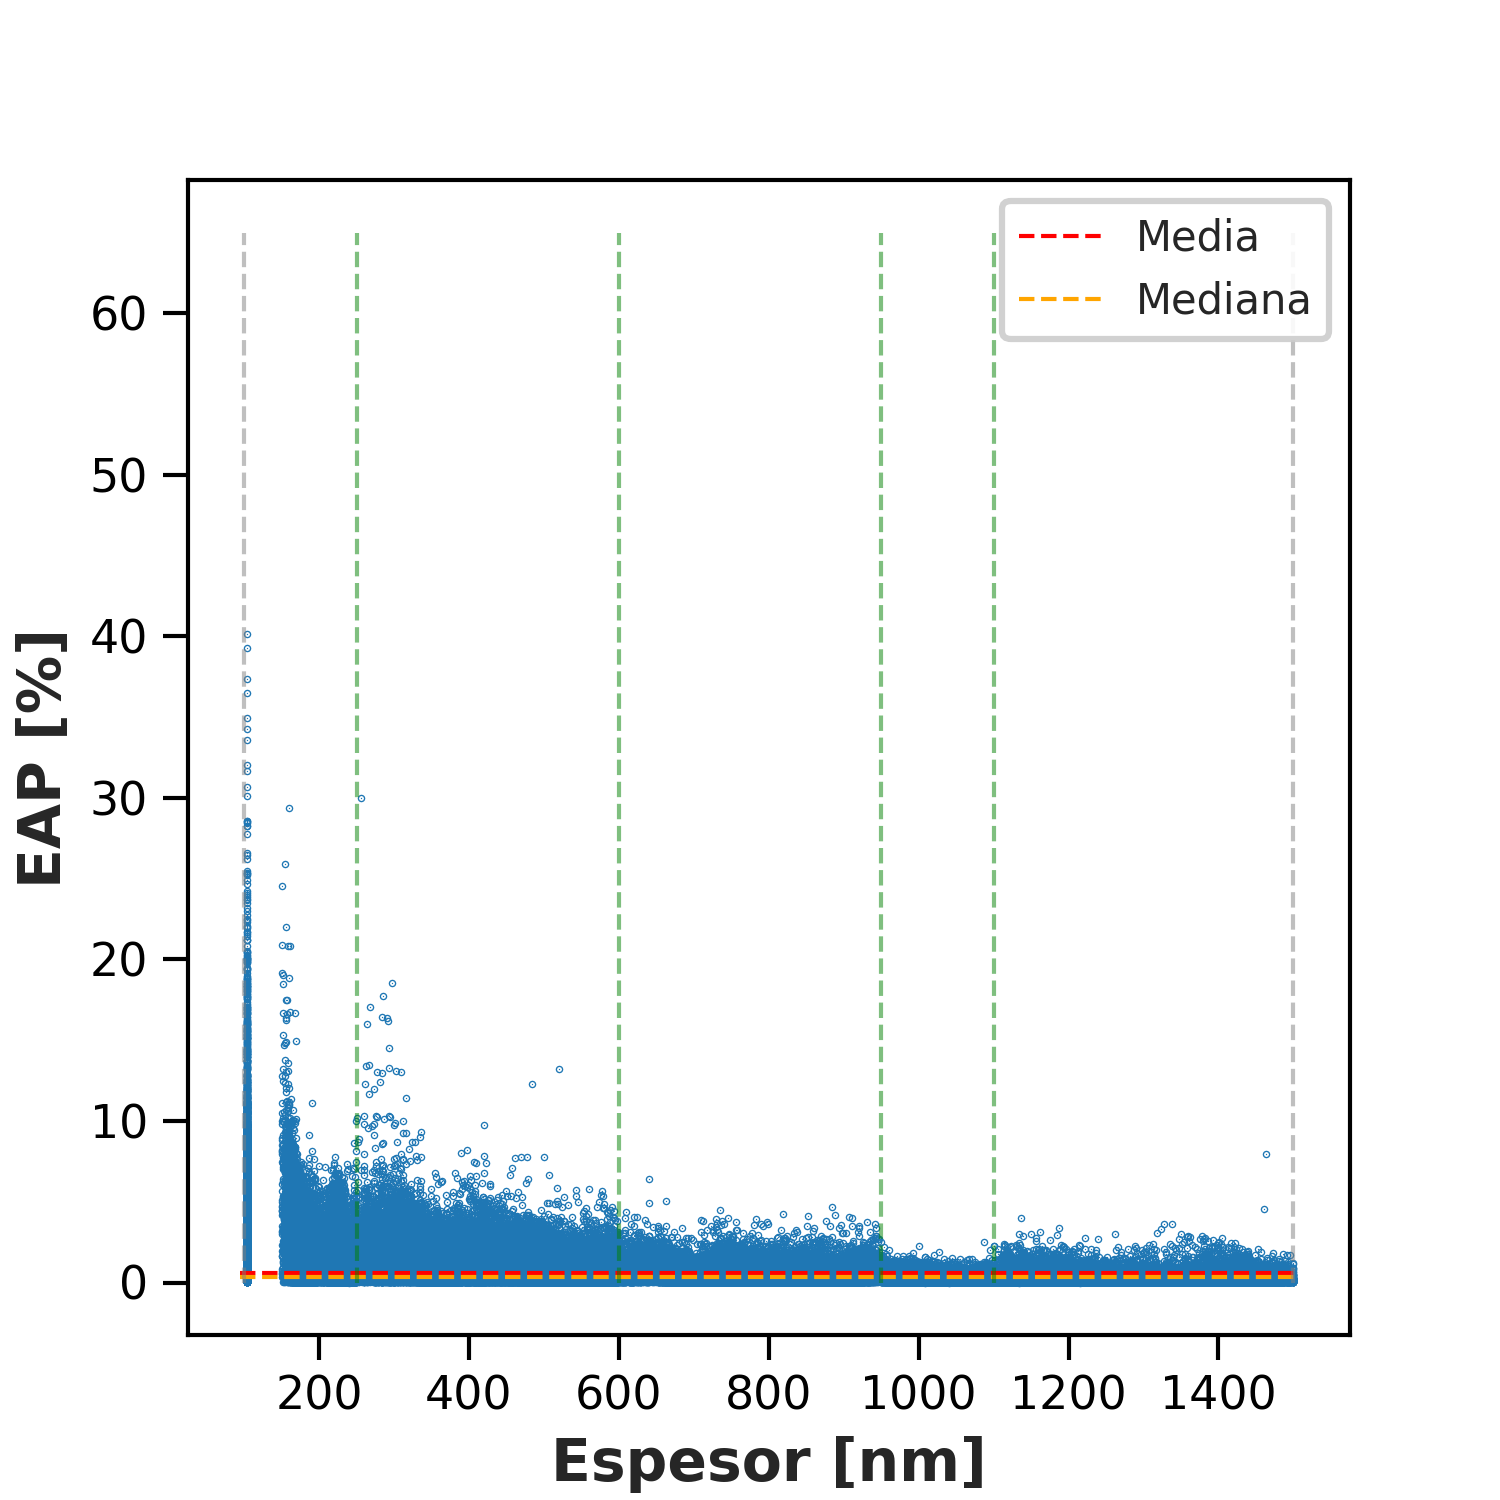
\includegraphics[width=0.48\textwidth]{train_error.png}
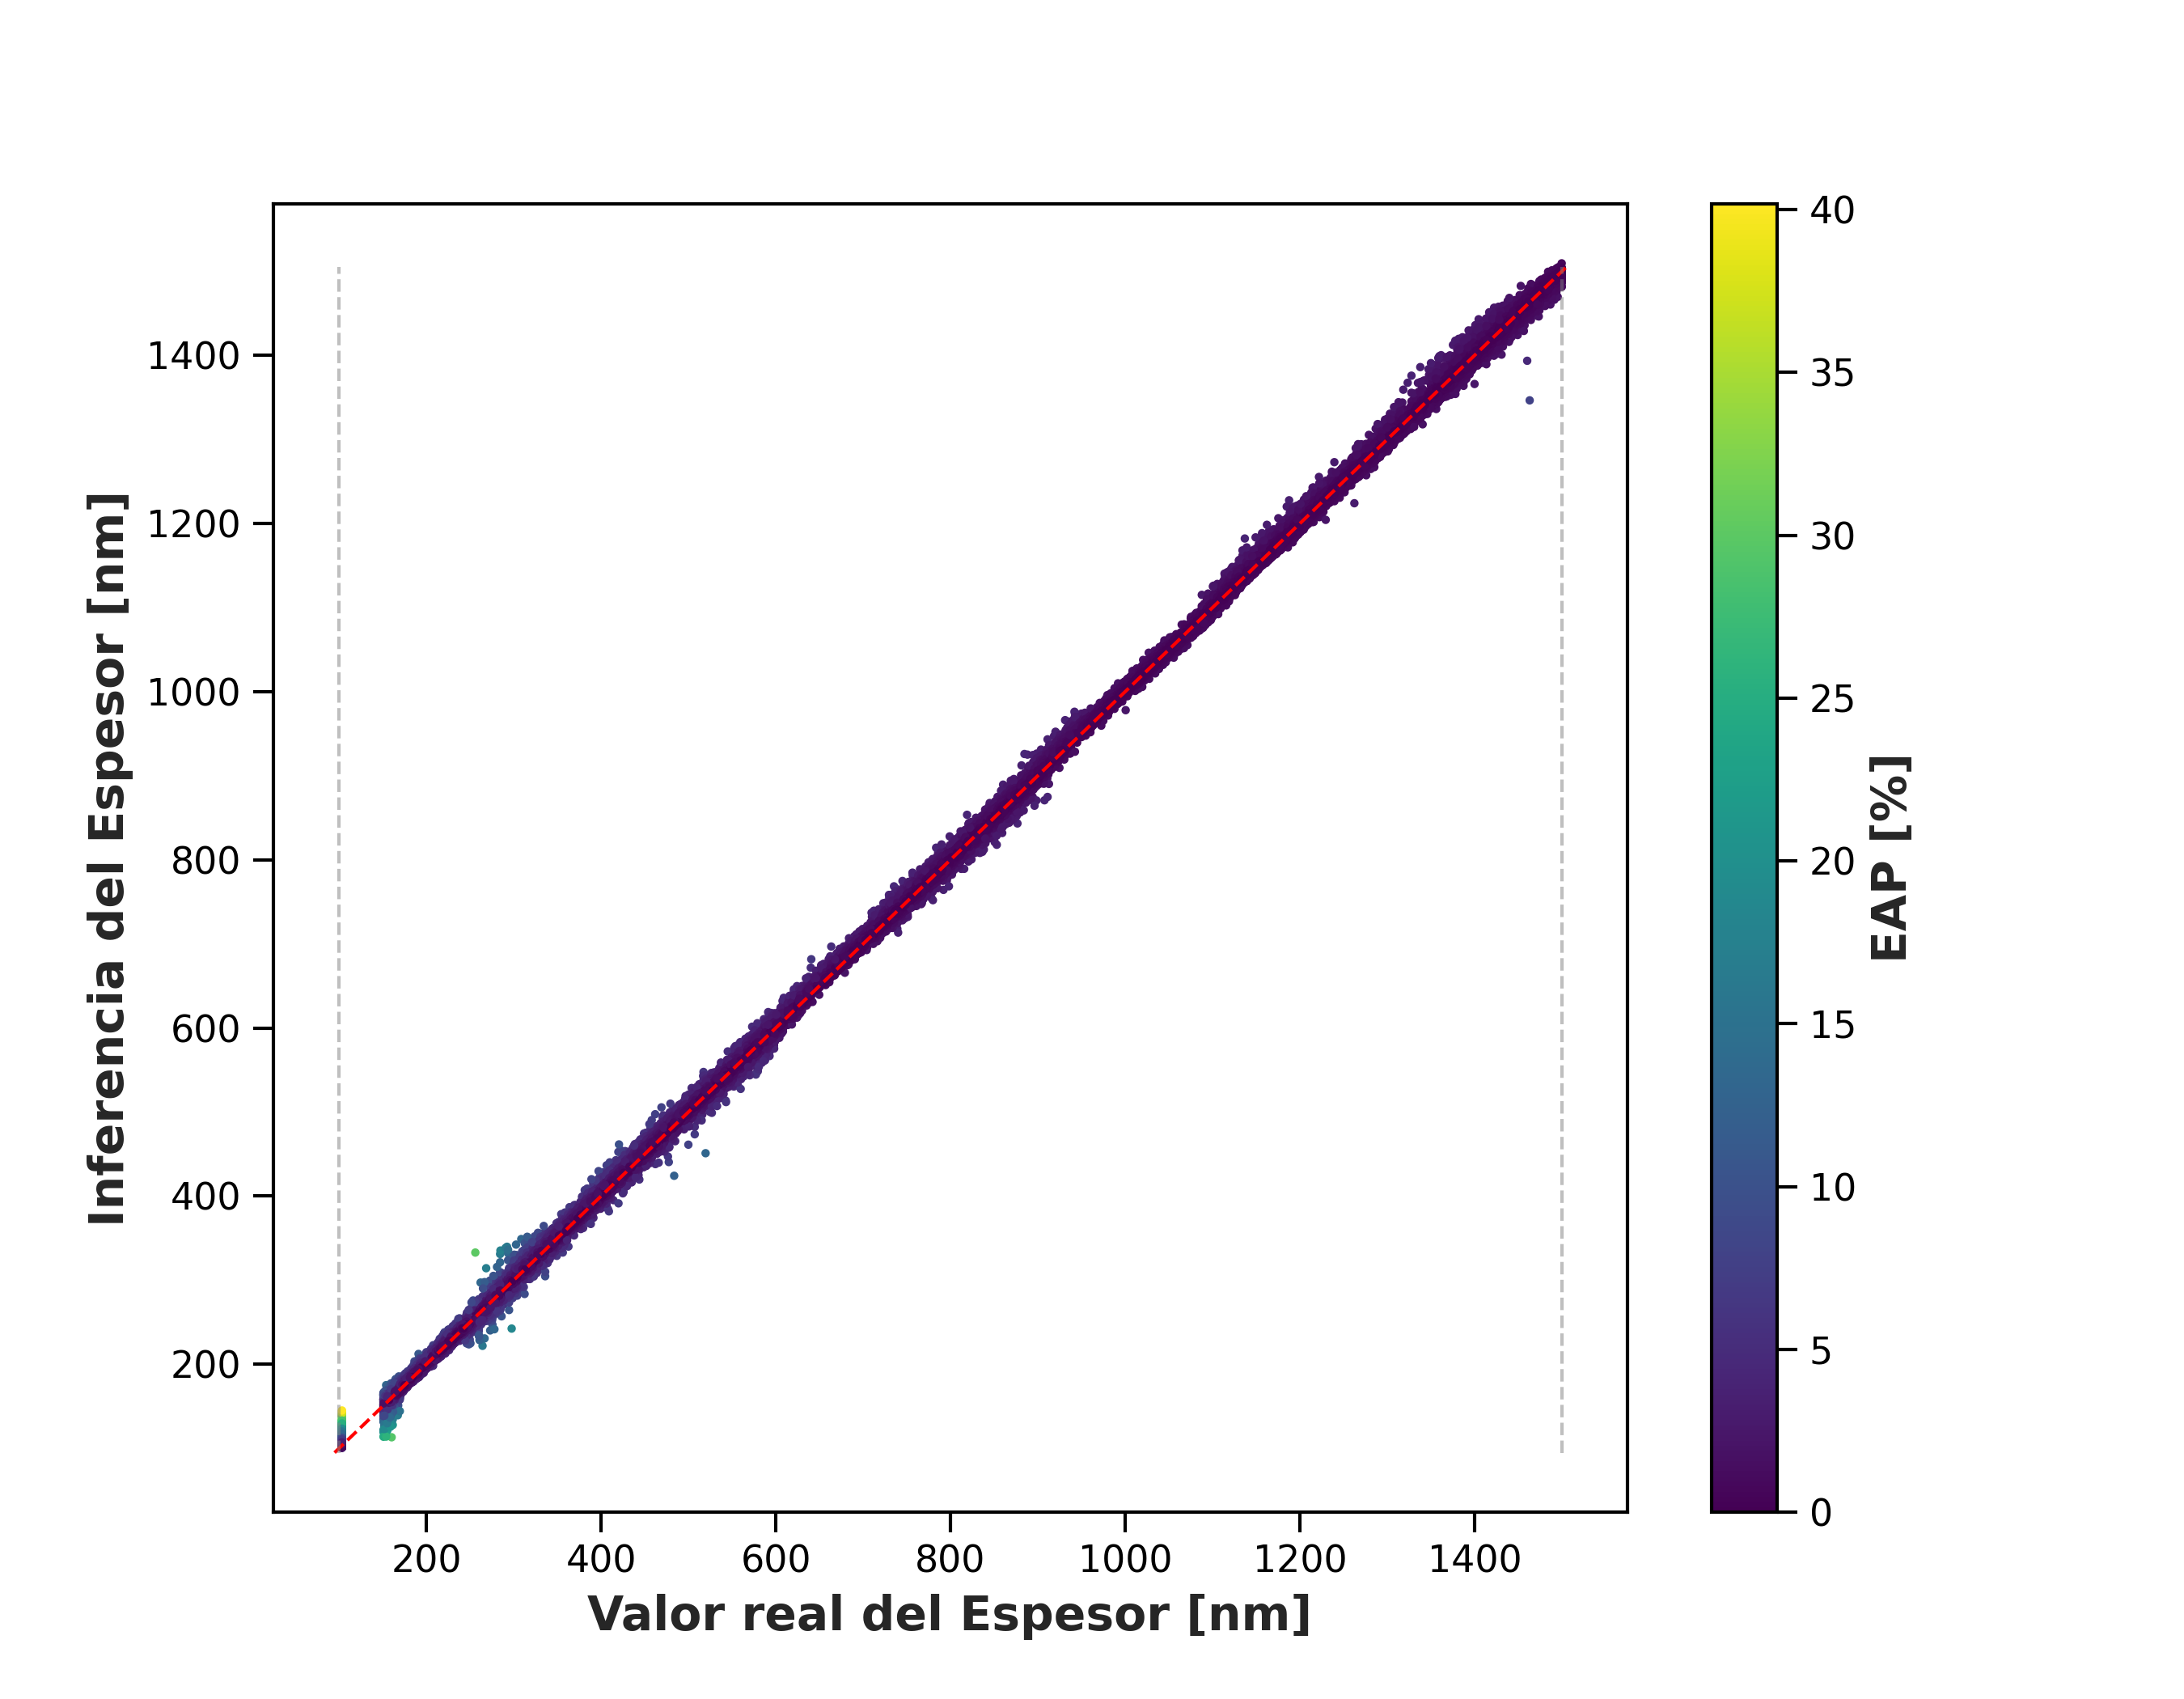
\includegraphics[width=0.48\textwidth]{train_comparsion_true_preds.png}
\caption{División Train: error de predicción (izq.) y comparación valores reales vs predichos (der.).}
\label{fig:train-1}
\end{figure}

\begin{figure}[htbp]
\centering
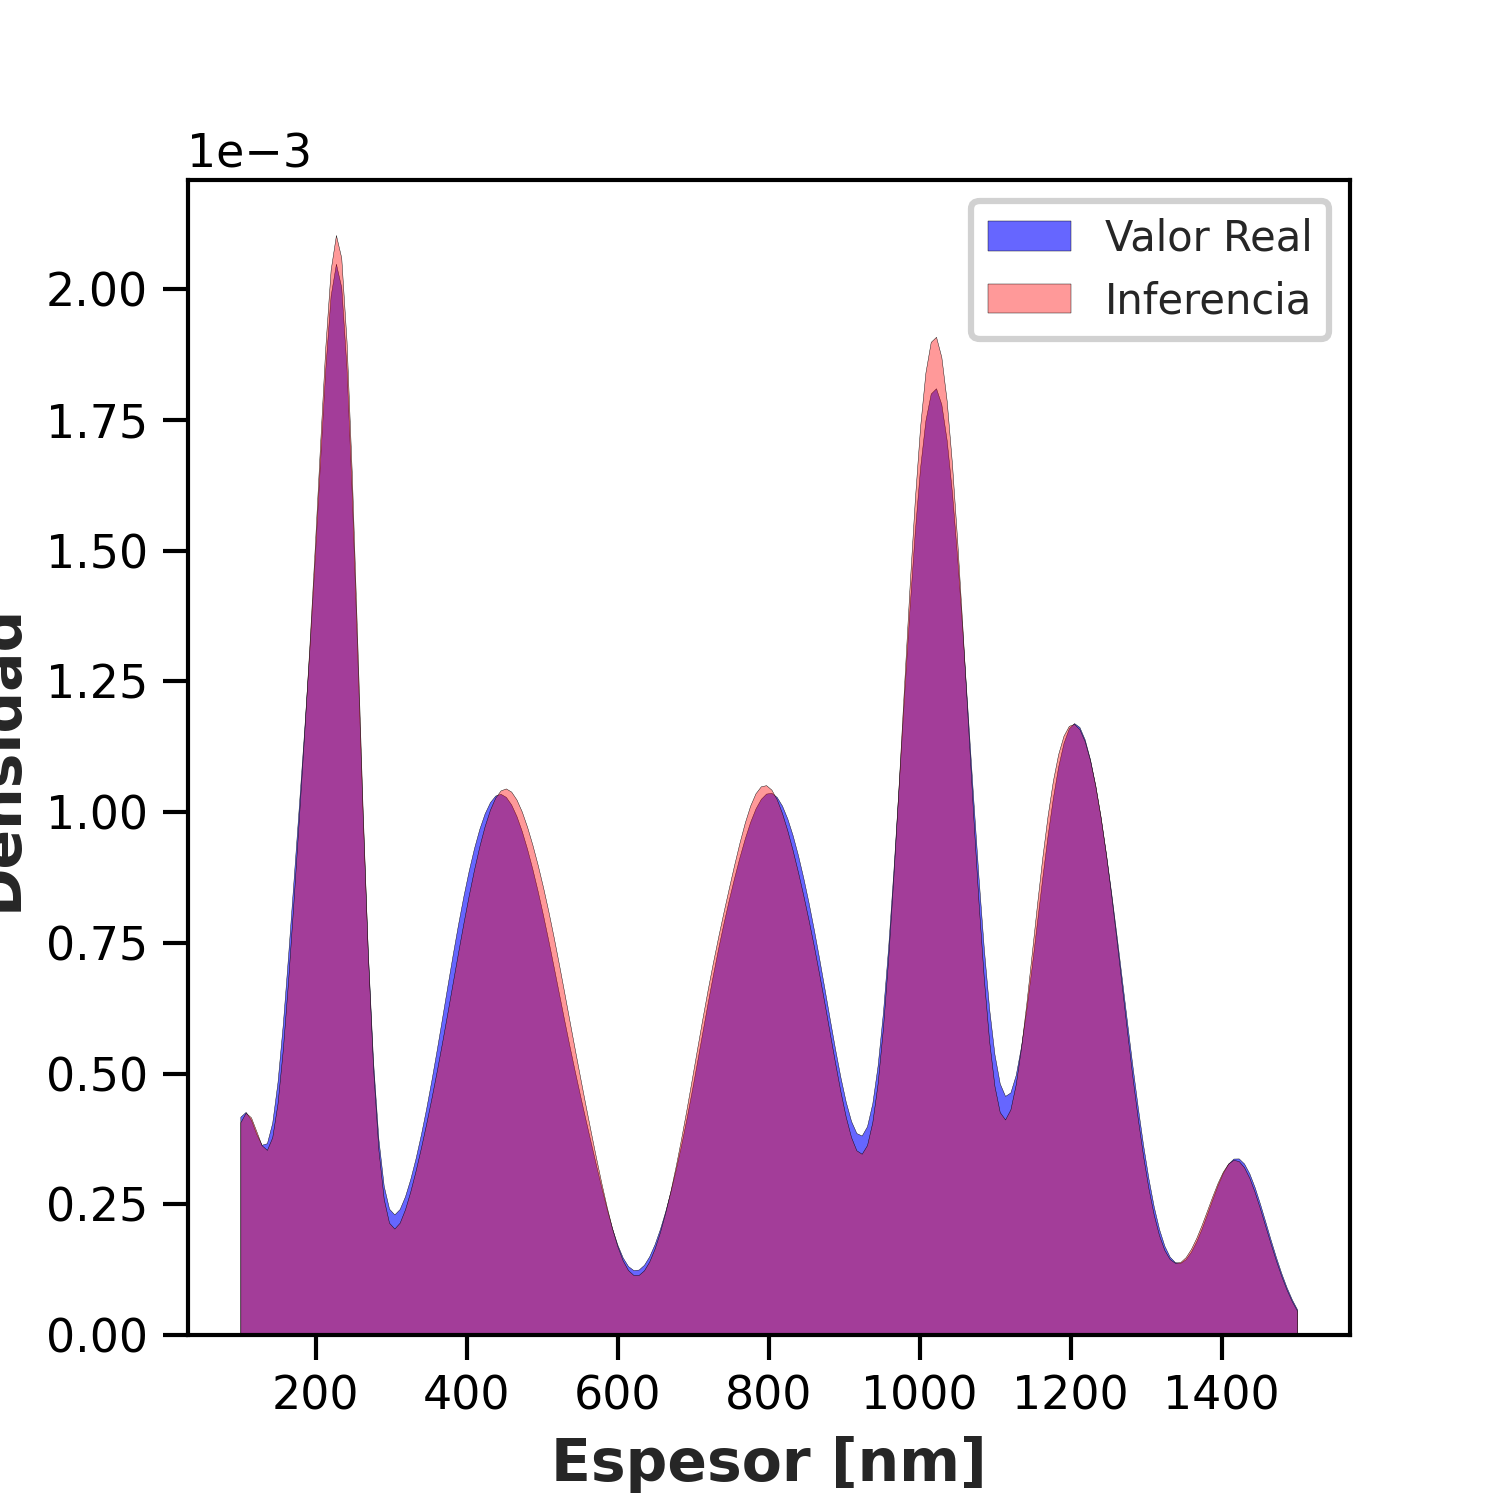
\includegraphics[width=0.48\textwidth]{train_two_dist.png}
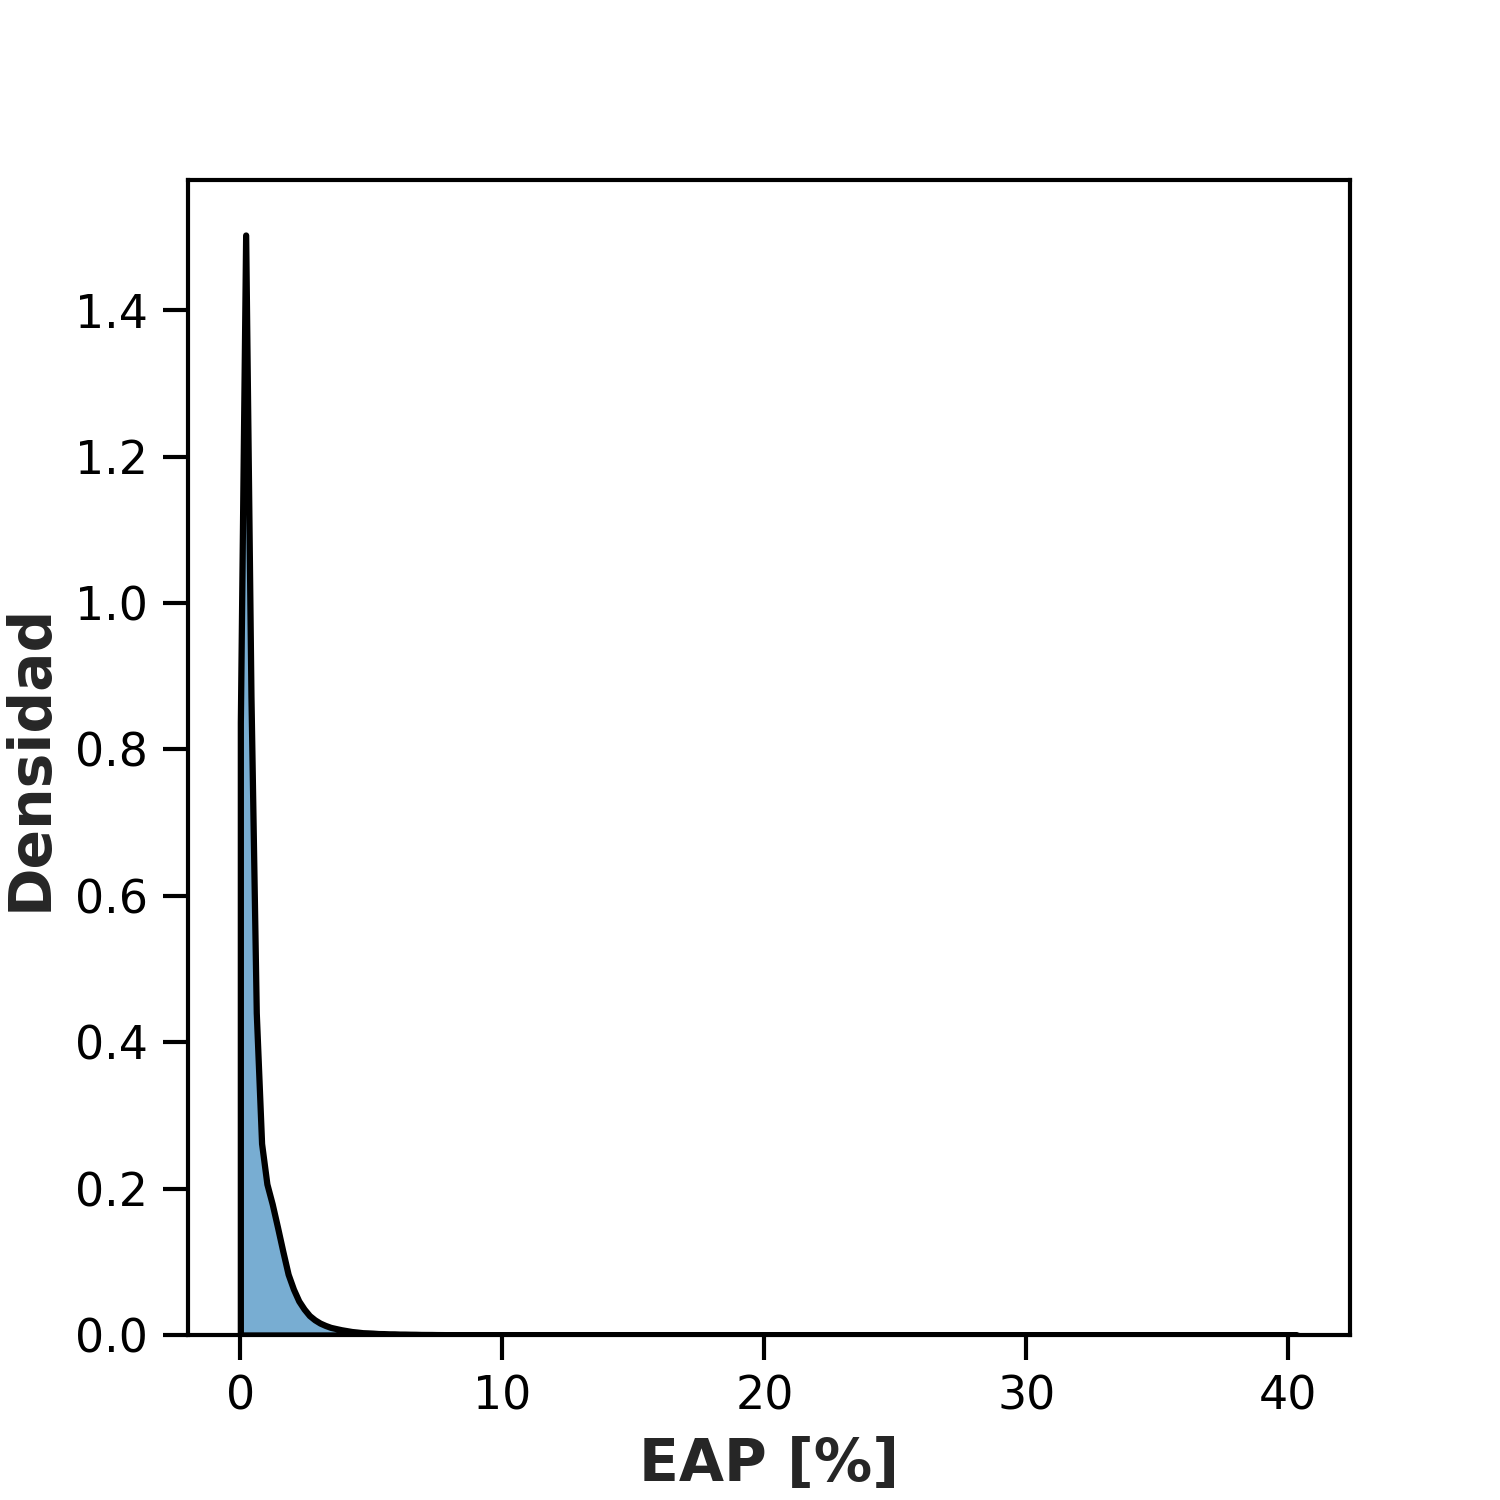
\includegraphics[width=0.48\textwidth]{train_dist_ape.png}
\caption{División Train: distribuciones superpuestas (izq.) y distribución APE (der.).}
\label{fig:train-2}
\end{figure}

\begin{figure}[htbp]
\centering
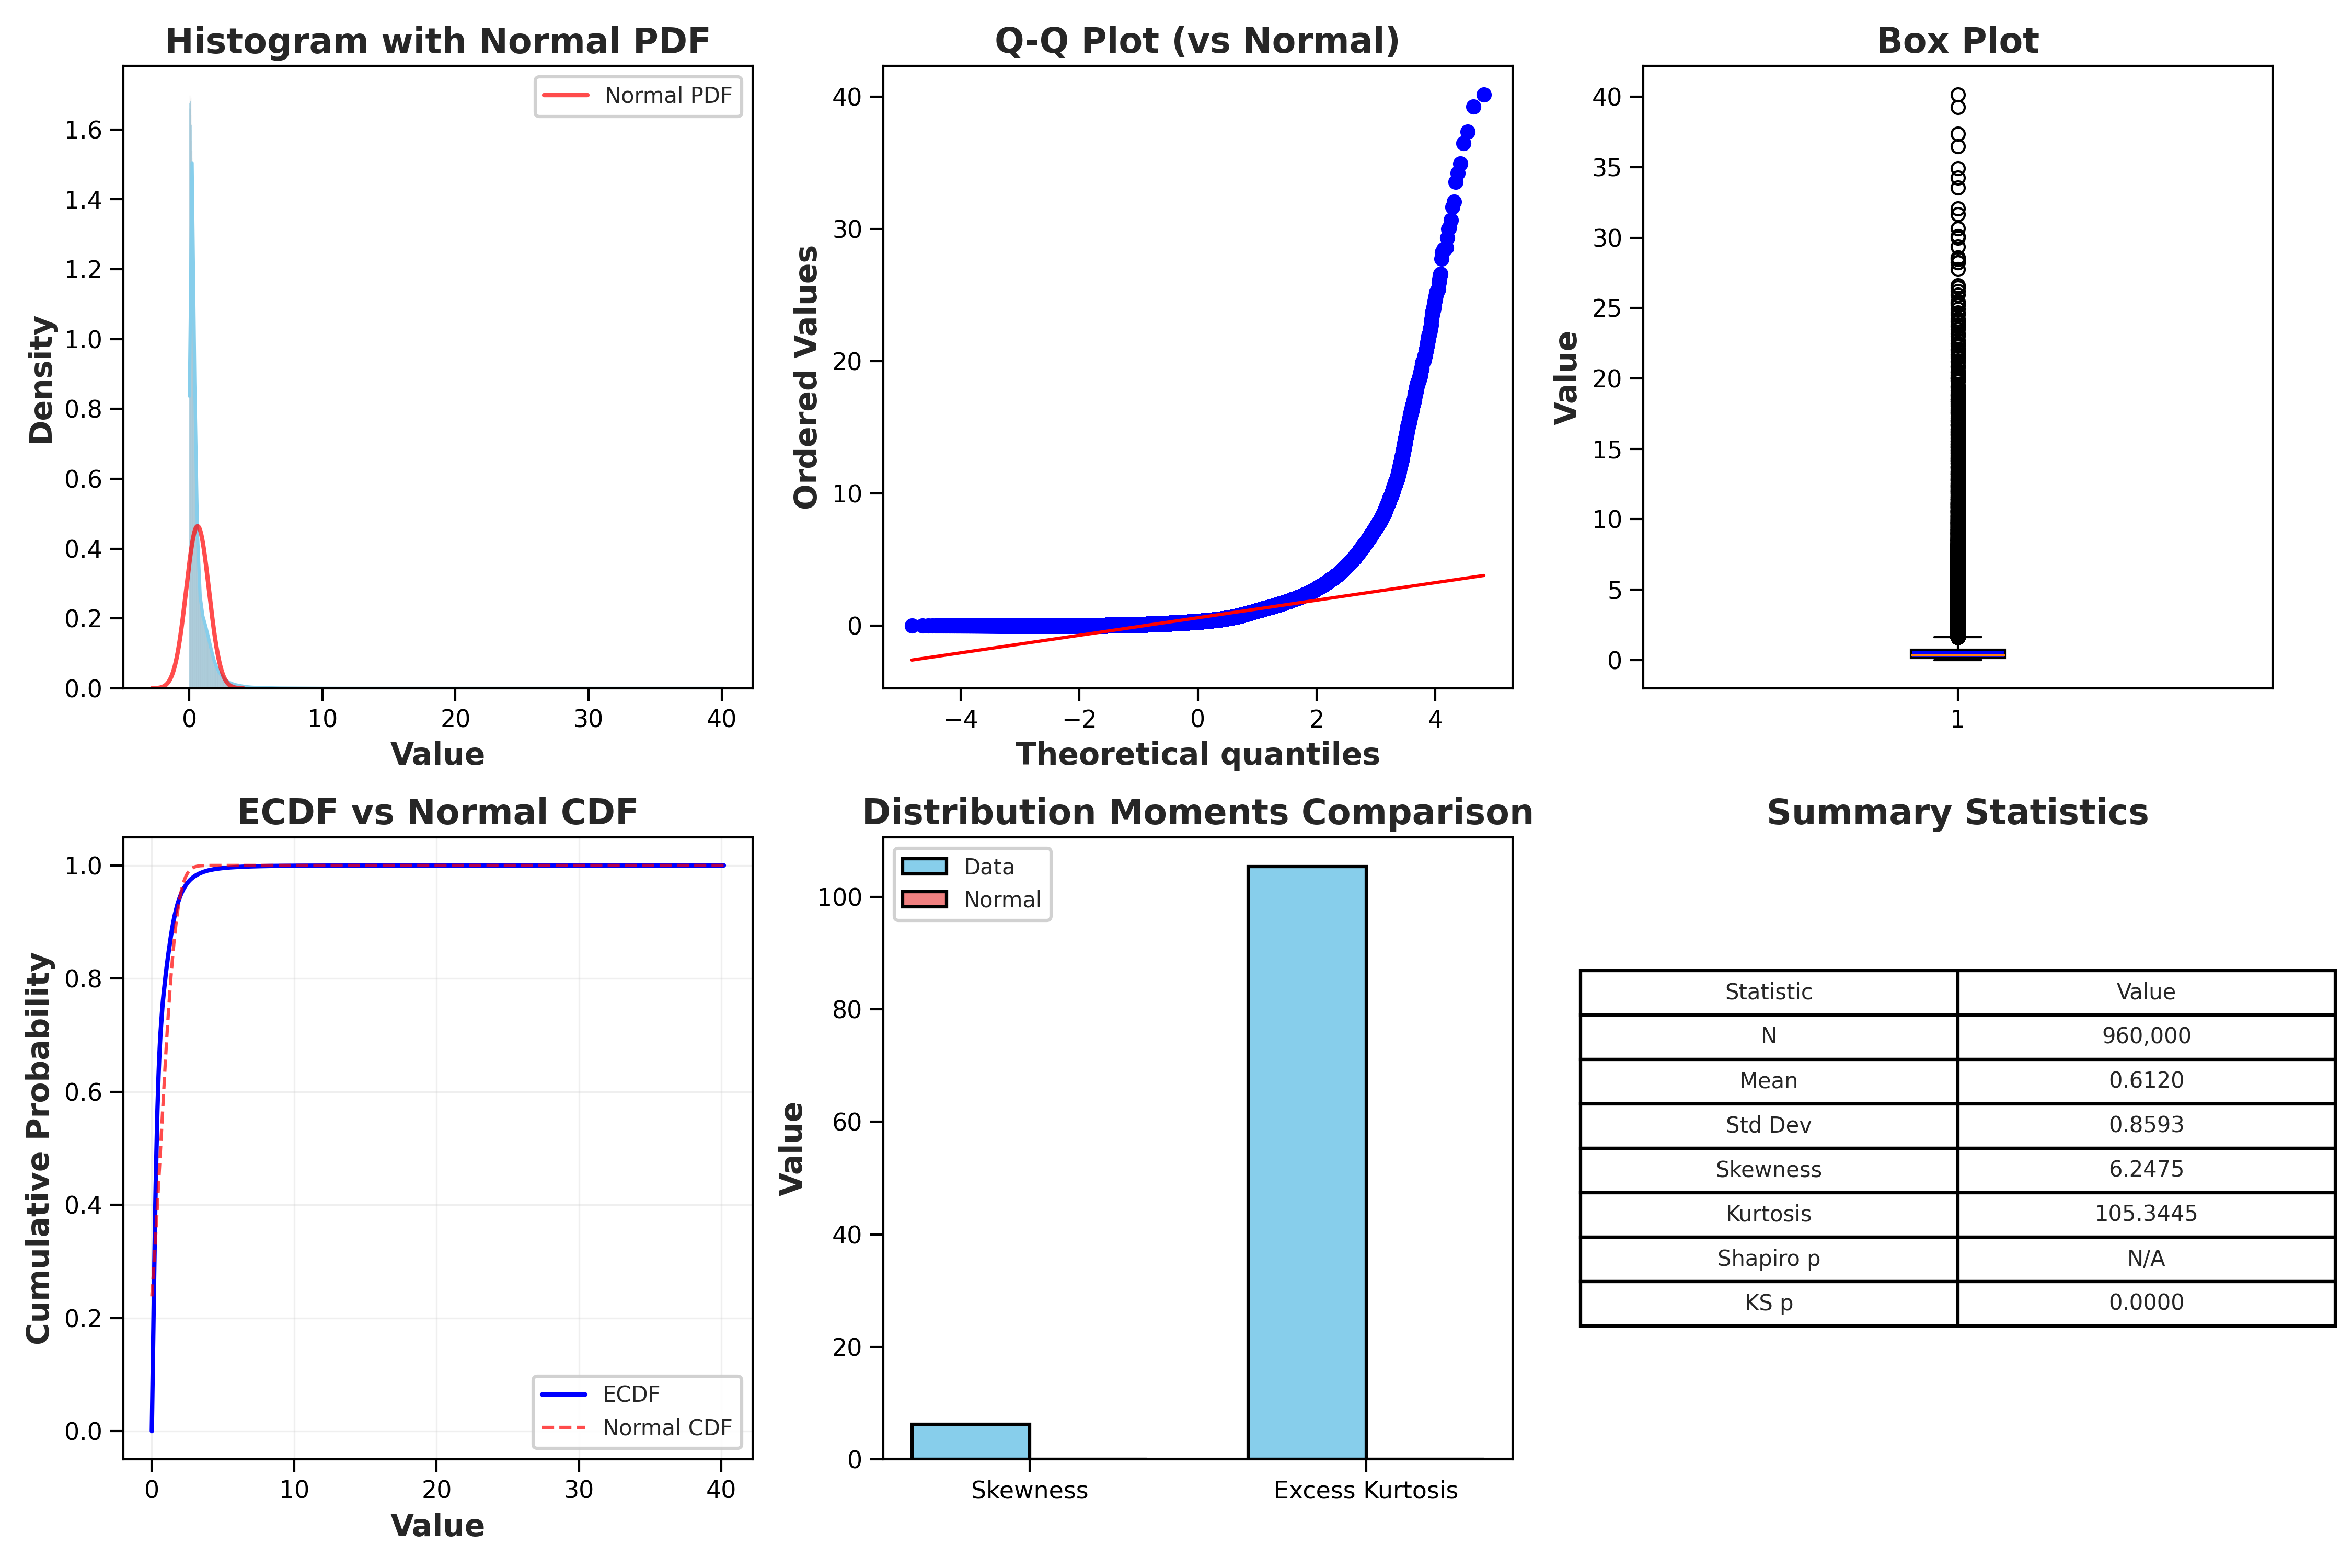
\includegraphics[width=0.48\textwidth]{train_dist_analysis_ape.png}
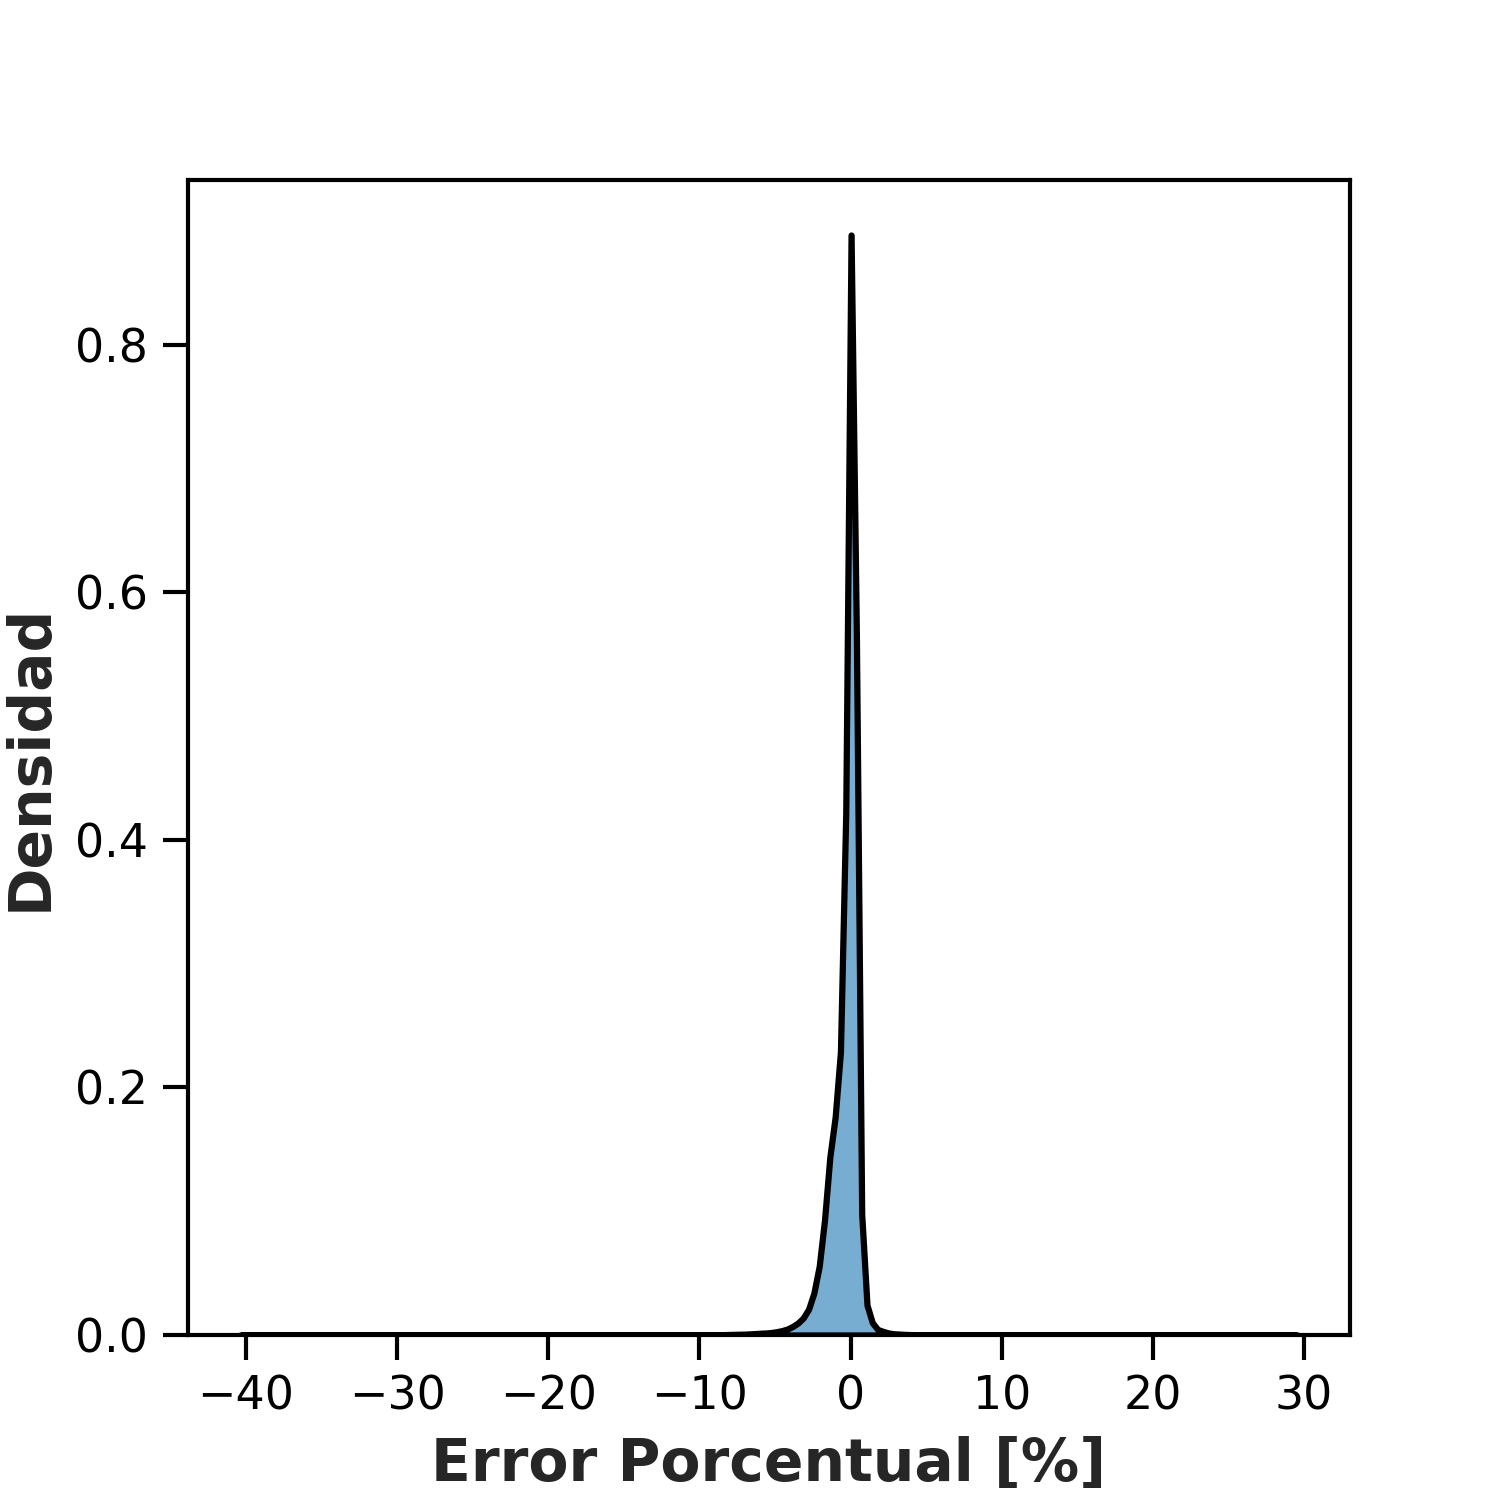
\includegraphics[width=0.48\textwidth]{train_dist_ep.png}
\caption{División Train: análisis diagnóstico APE (izq.) y distribución PE (der.).}
\label{fig:train-3}
\end{figure}

\begin{figure}[htbp]
\centering
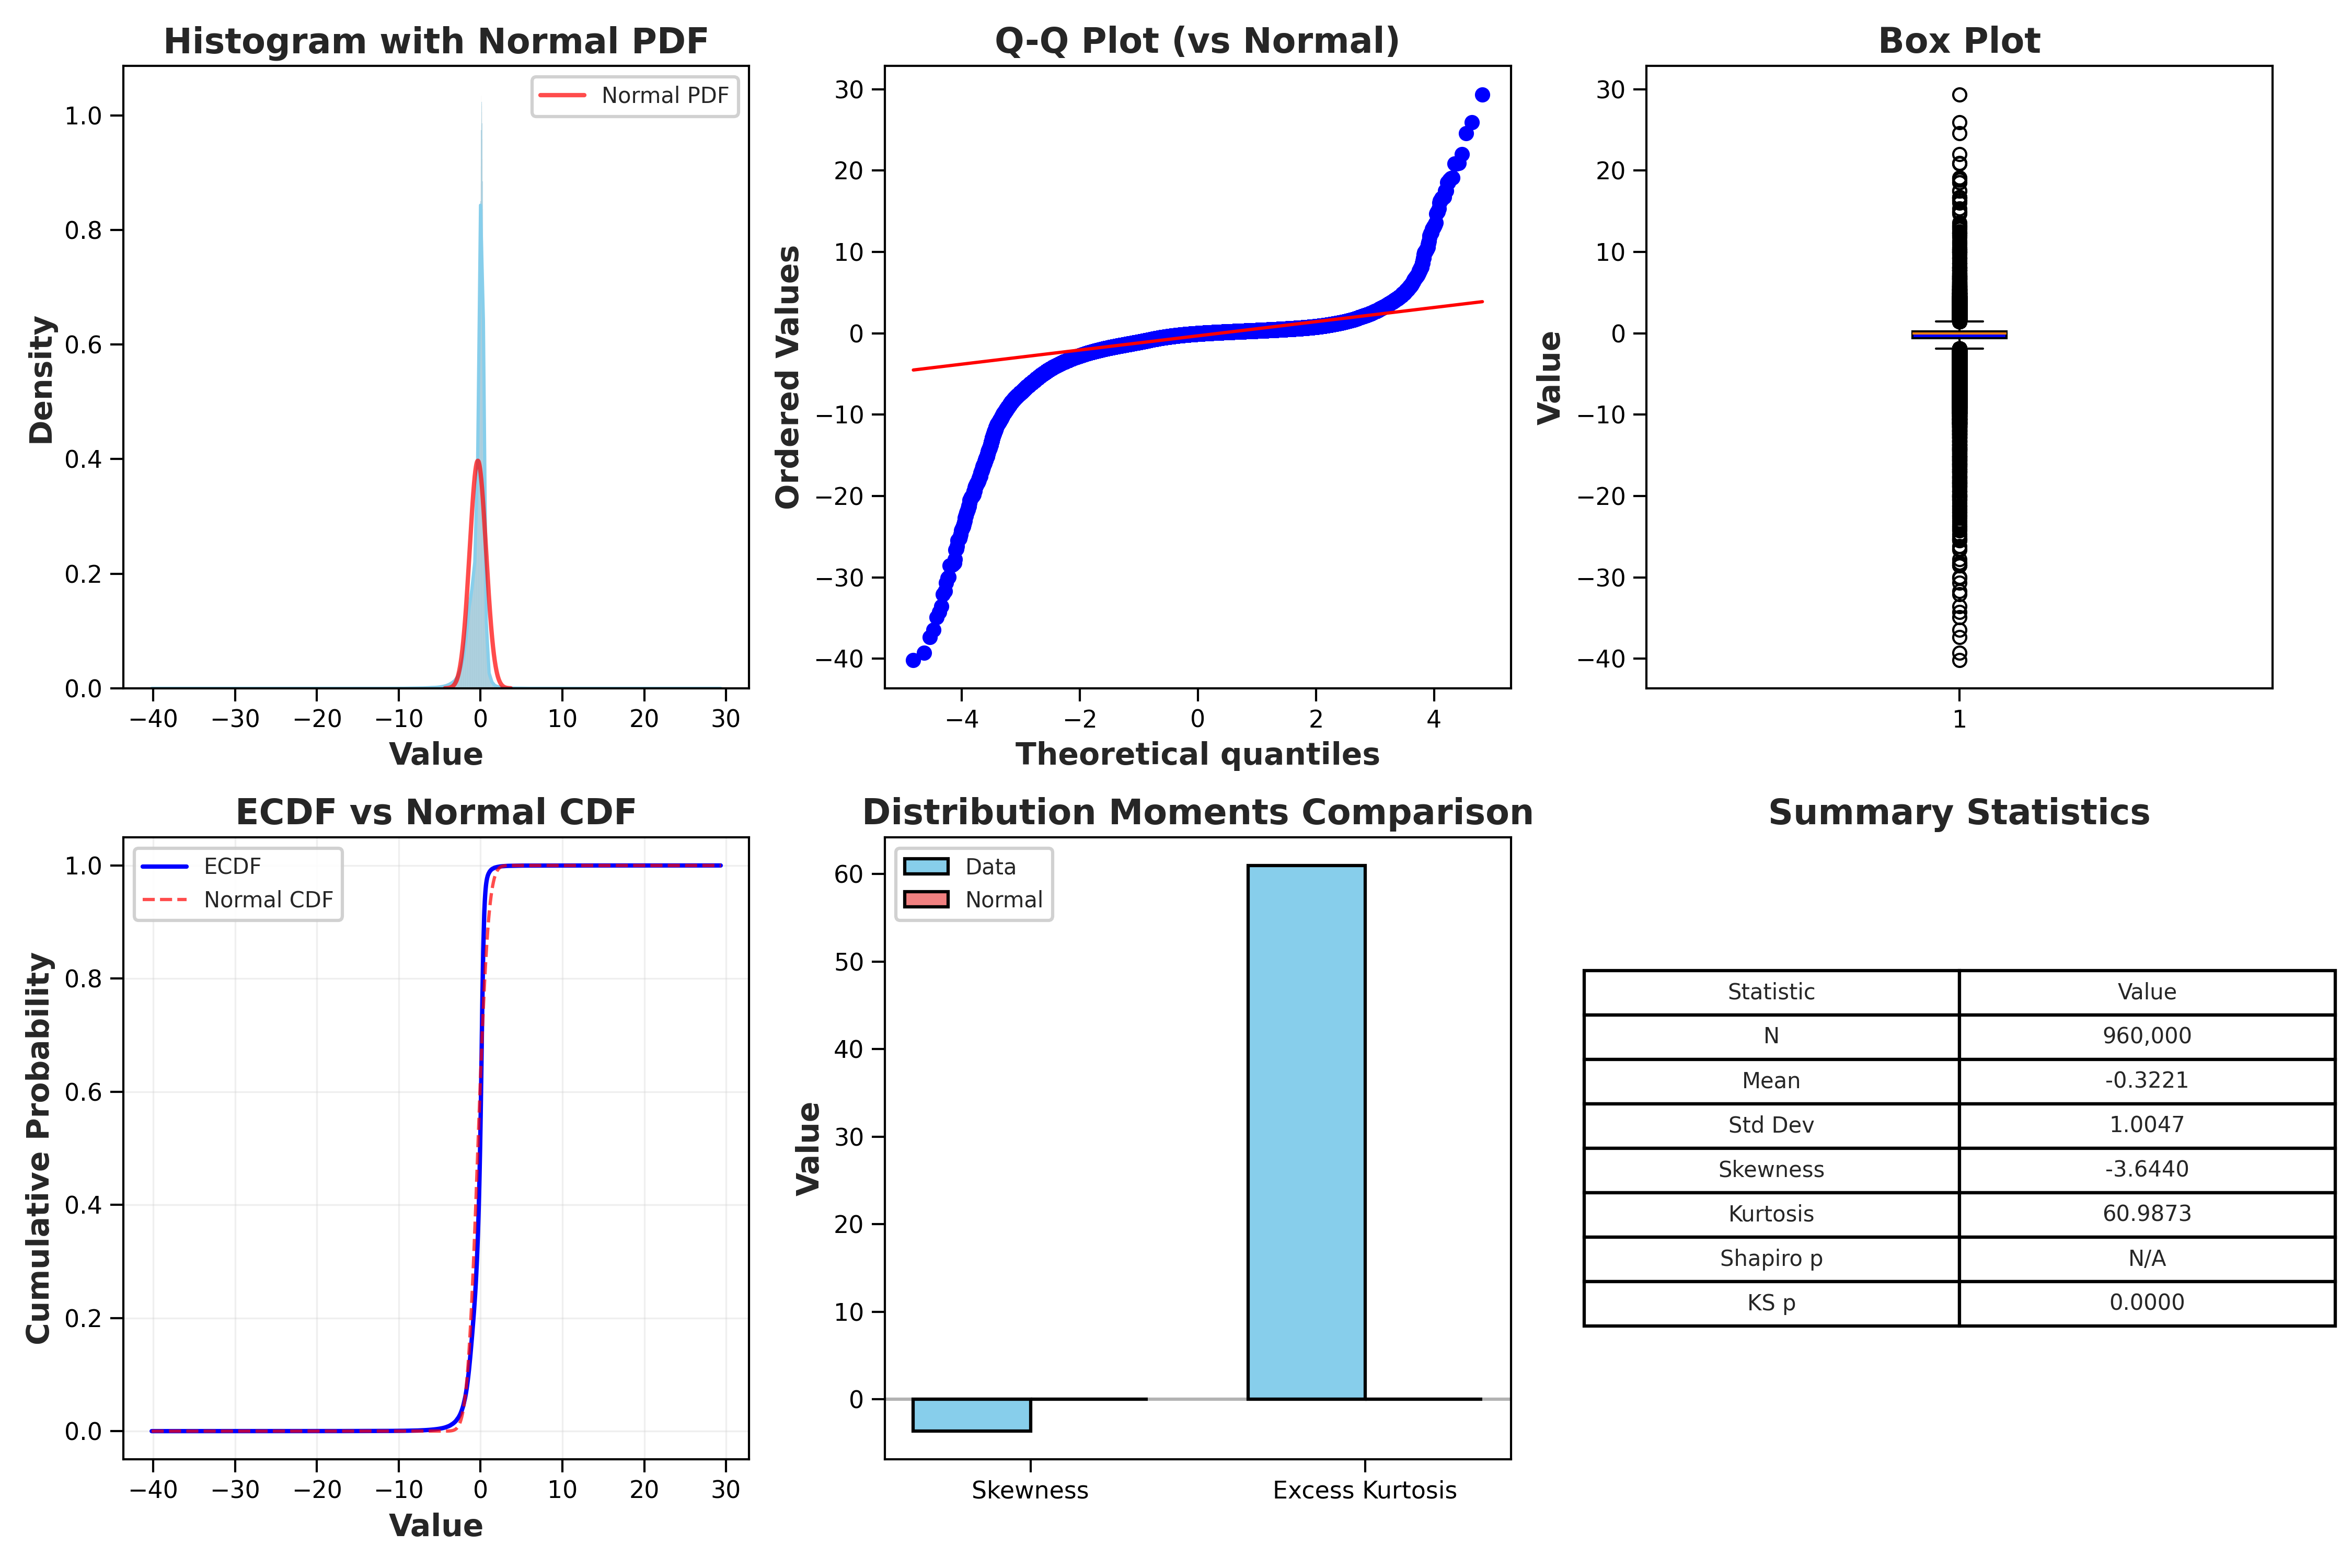
\includegraphics[width=0.7\textwidth]{train_dist_analysis_pe.png}
\caption{División Train: análisis diagnóstico PE (6 paneles).}
\label{fig:train-4}
\end{figure}

%%%%%%%%%%%%%%%%%%%%%%%%%%%%%%%%%%%%%%%%%%%%%%%%%%%%%%%%%%%%%%
\subsection{División Validación ($N = 120{,}000$)}
%%%%%%%%%%%%%%%%%%%%%%%%%%%%%%%%%%%%%%%%%%%%%%%%%%%%%%%%%%%%%%

\subsubsection{Métricas de Error}

\begin{table}[htbp]
\centering
\caption{Métricas de error — División Validación.}
\label{tab:val-metrics}
\begin{tabular}{ll}
\hline
Métrica & Valor \\
\hline
MAE  & 2.91~nm \\
MSE  & 14.80~nm$^2$ \\
RMSE & 3.85~nm \\
MAPE & 0.61\% \\
$R^2$ & 0.9999 \\
\hline
\end{tabular}
\end{table}

\subsubsection{Distribución APE (Error Porcentual Absoluto)}

\begin{table}[htbp]
\centering
\caption{Estadísticos de la distribución APE — Validación.}
\label{tab:val-ape}
\begin{tabular}{ll}
\hline
Estadístico & Valor \\
\hline
Media                    & 0.6095\% \\
Mediana                  & 0.3275\% \\
Desviación Estándar      & 0.8552\% \\
Asimetría (Skewness)     & 6.5218 (altamente sesgada, derecha) \\
Curtosis (Exceso)        & 124.7084 (leptocúrtica) \\
Outliers (IQR)           & 10,465 (8.72\%) \\
\hline
\end{tabular}
\end{table}

\textbf{Normalidad:} Rechazada por todas las pruebas (KS $D = 0.2380$, AD $A^2 = 11{,}329.0$, JB $= 7.86 \times 10^7$, todos $p \approx 0$).

\subsubsection{Distribución PE (Error Porcentual)}

\begin{table}[htbp]
\centering
\caption{Estadísticos de la distribución PE — Validación.}
\label{tab:val-pe}
\begin{tabular}{ll}
\hline
Estadístico & Valor \\
\hline
Media                    & $-0.3186\%$ \\
Mediana                  & $-0.0446\%$ \\
Desviación Estándar      & 1.0007\% \\
Asimetría (Skewness)     & $-4.1251$ (altamente sesgada, izquierda) \\
Curtosis (Exceso)        & 70.9283 (leptocúrtica) \\
Outliers (IQR)           & 8,026 (6.69\%) \\
\hline
\end{tabular}
\end{table}

\subsubsection{Figuras — División Validación}

\begin{figure}[htbp]
\centering
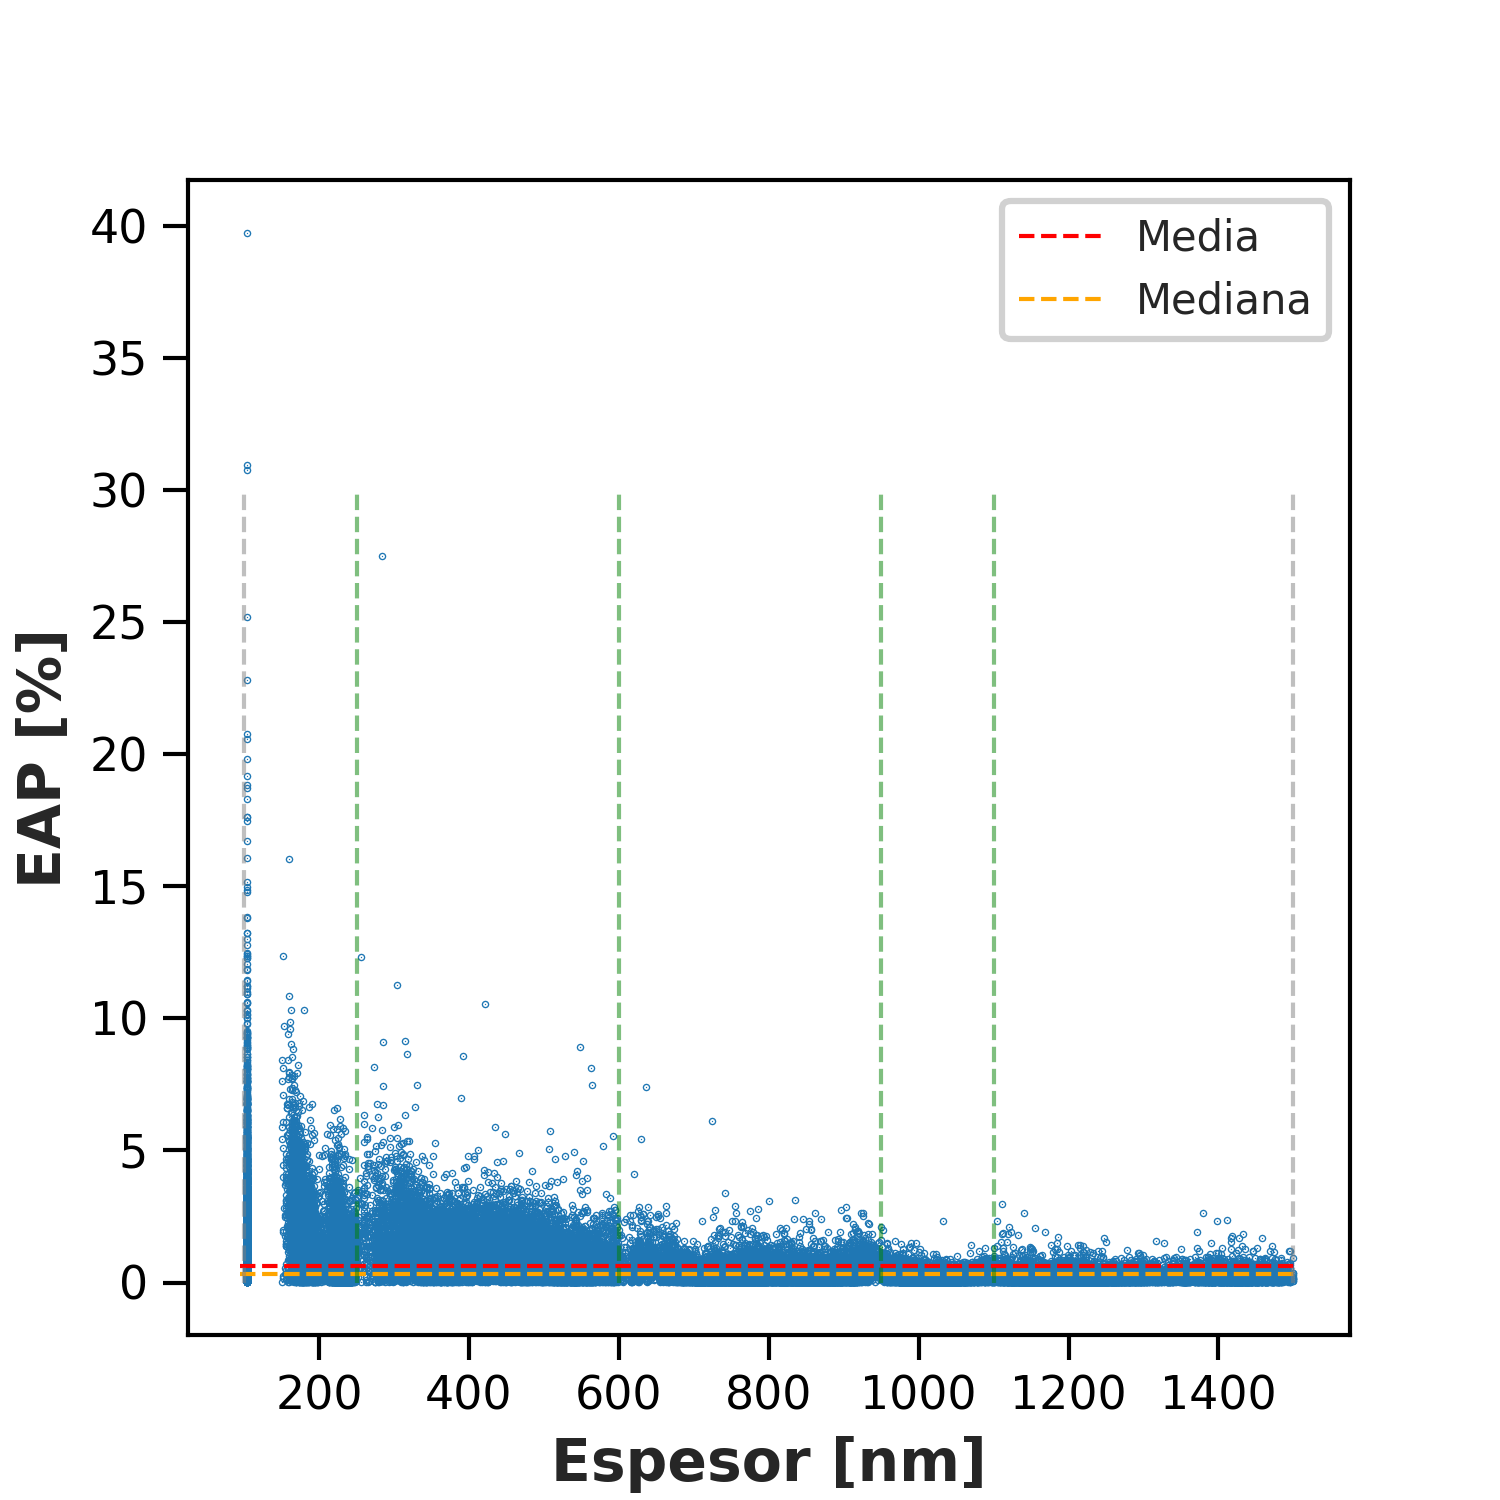
\includegraphics[width=0.48\textwidth]{val_error.png}
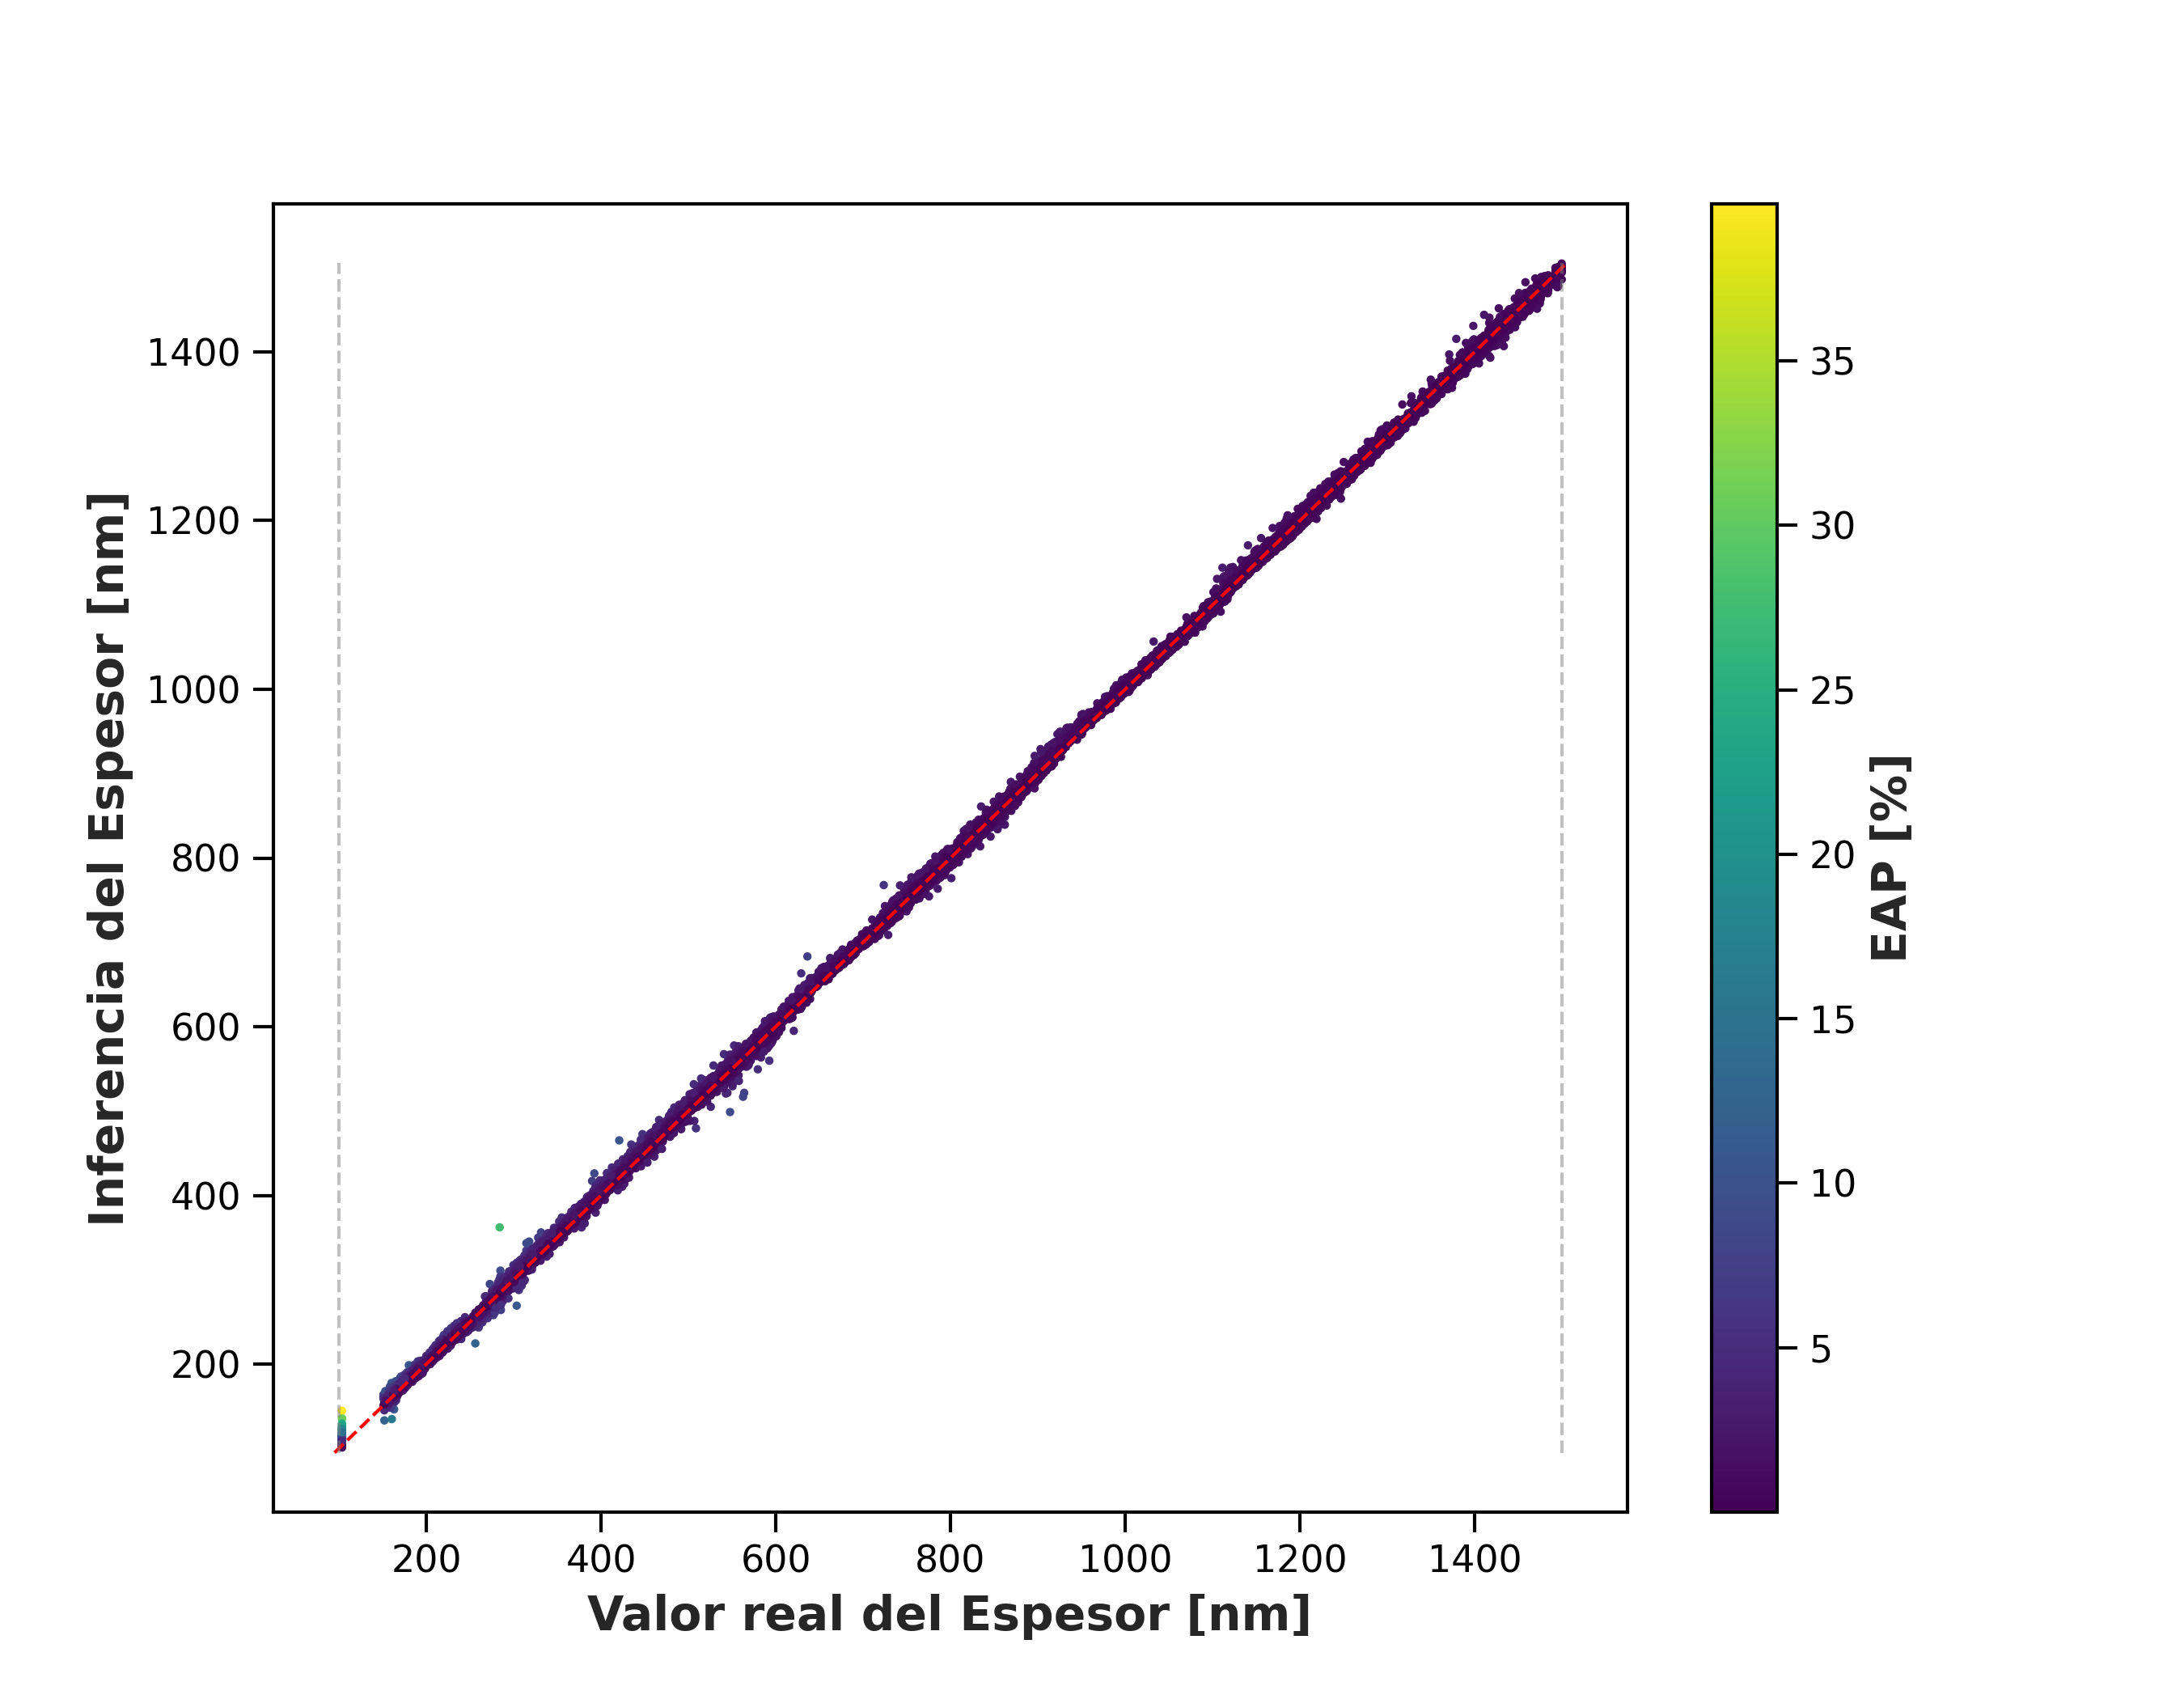
\includegraphics[width=0.48\textwidth]{val_comparsion_true_preds.png}
\caption{División Validación: error de predicción (izq.) y comparación real vs predicho (der.).}
\label{fig:val-1}
\end{figure}

\begin{figure}[htbp]
\centering
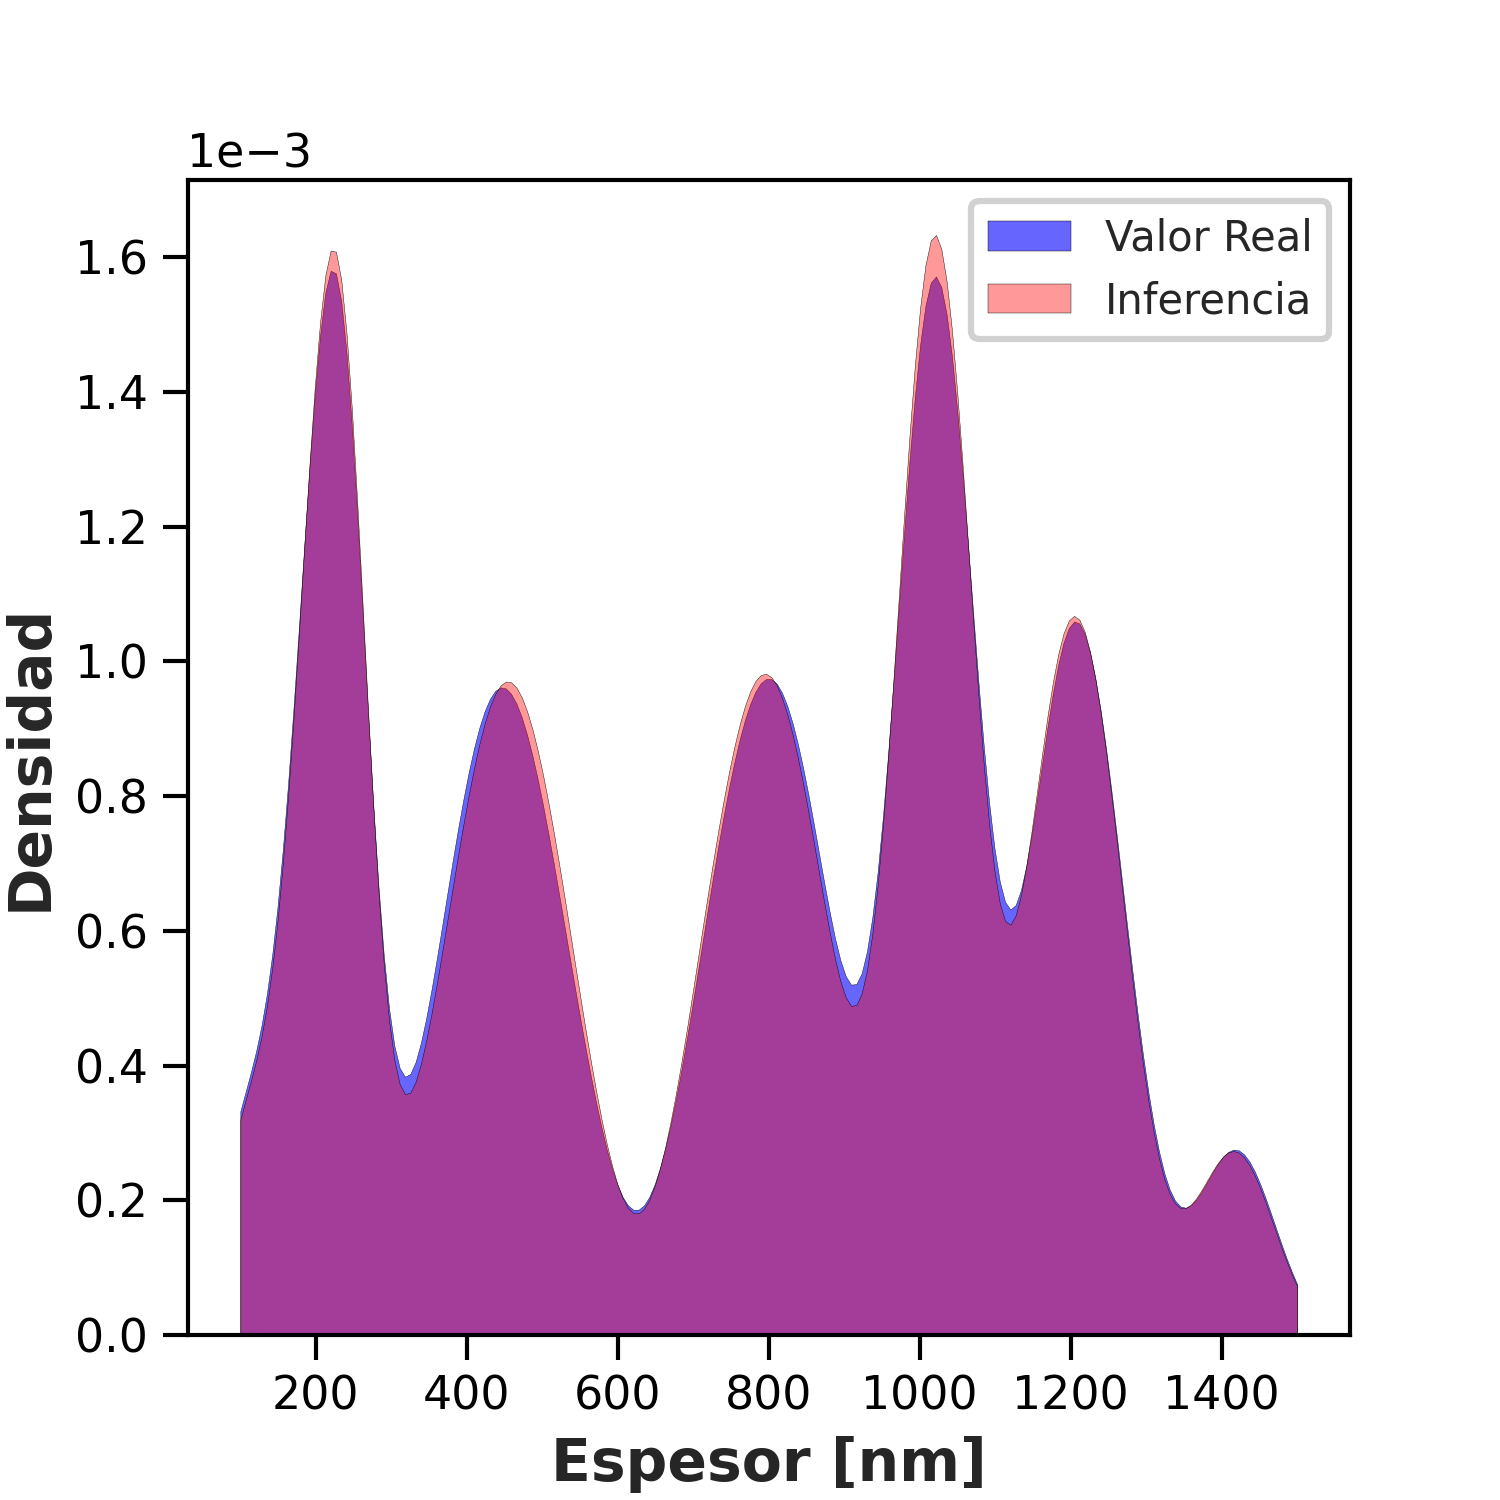
\includegraphics[width=0.48\textwidth]{val_two_dist.png}
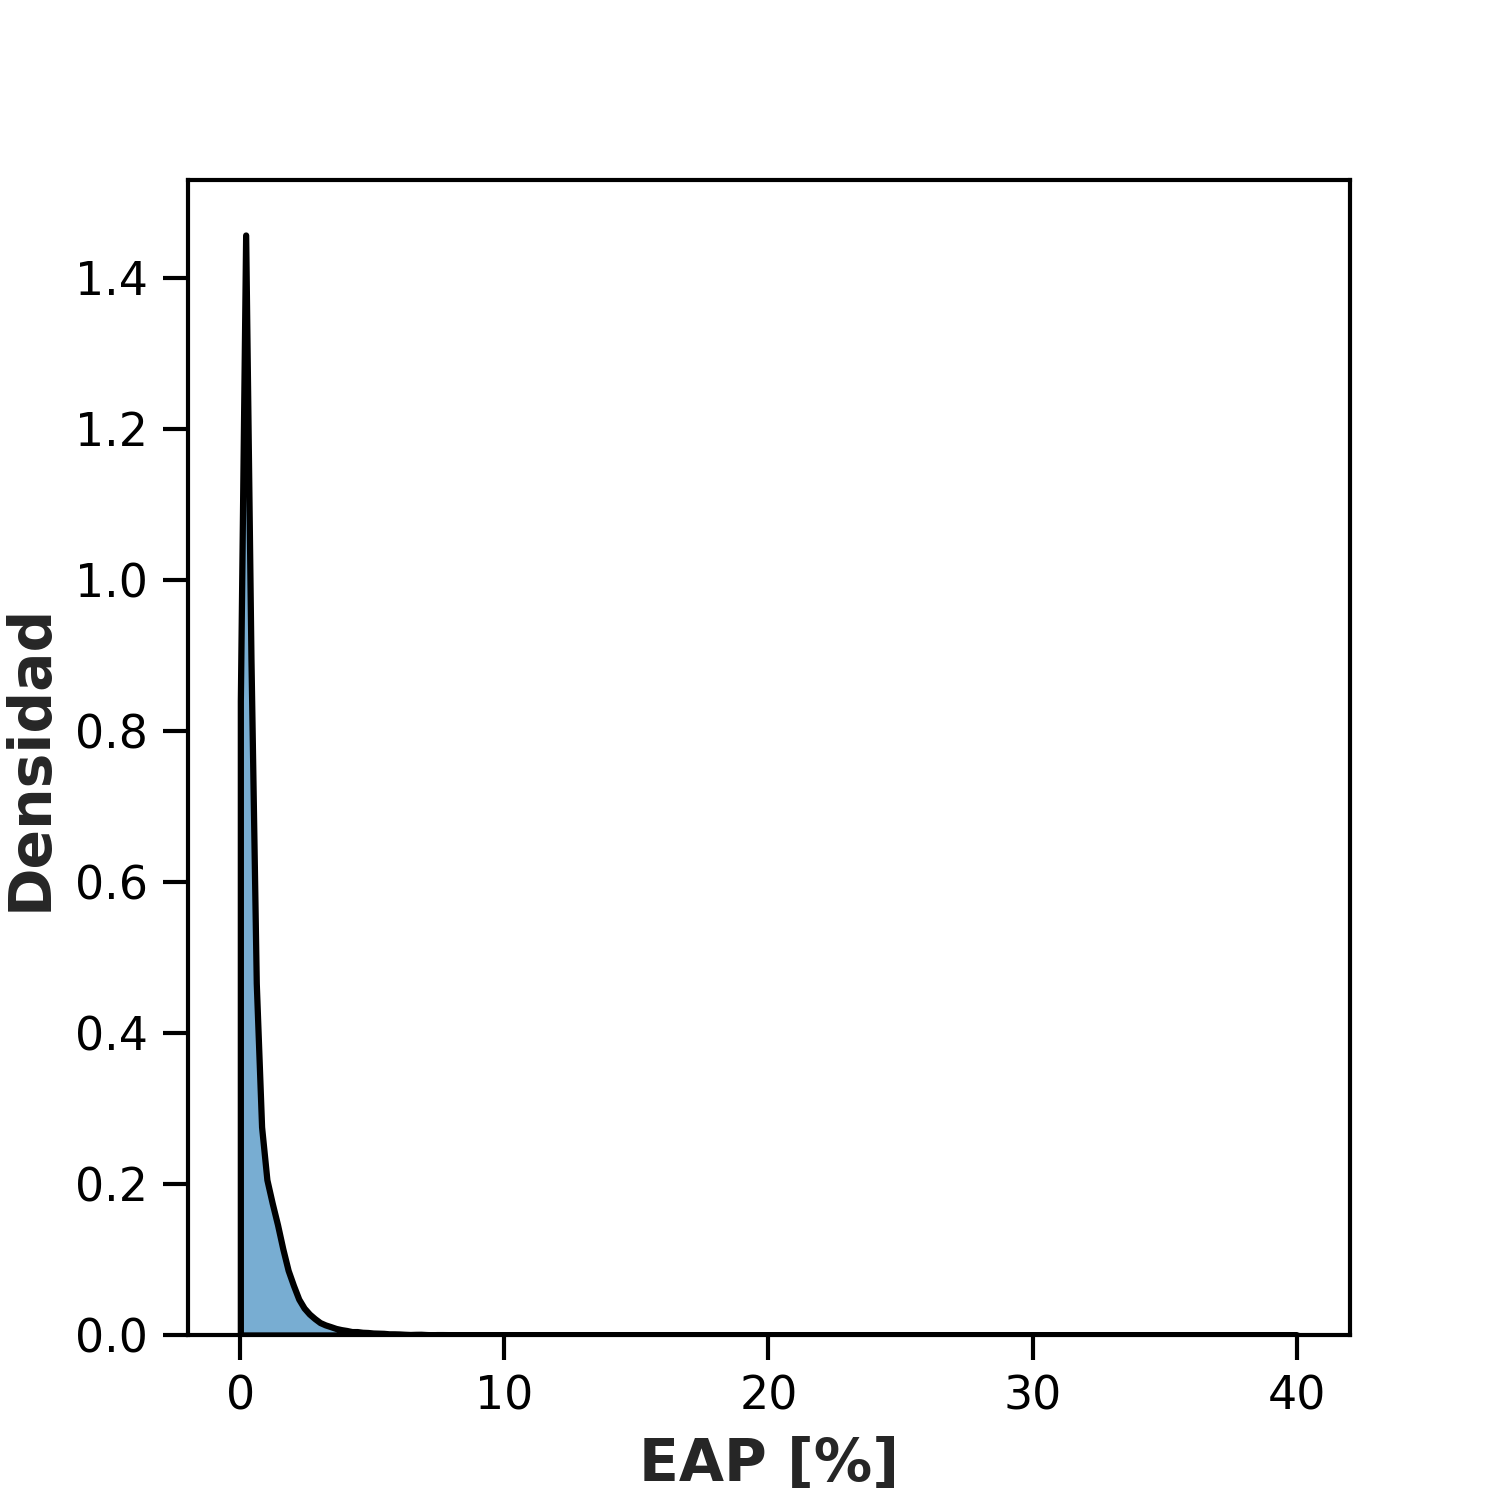
\includegraphics[width=0.48\textwidth]{val_dist_ape.png}
\caption{División Validación: distribuciones superpuestas (izq.) y distribución APE (der.).}
\label{fig:val-2}
\end{figure}

\begin{figure}[htbp]
\centering
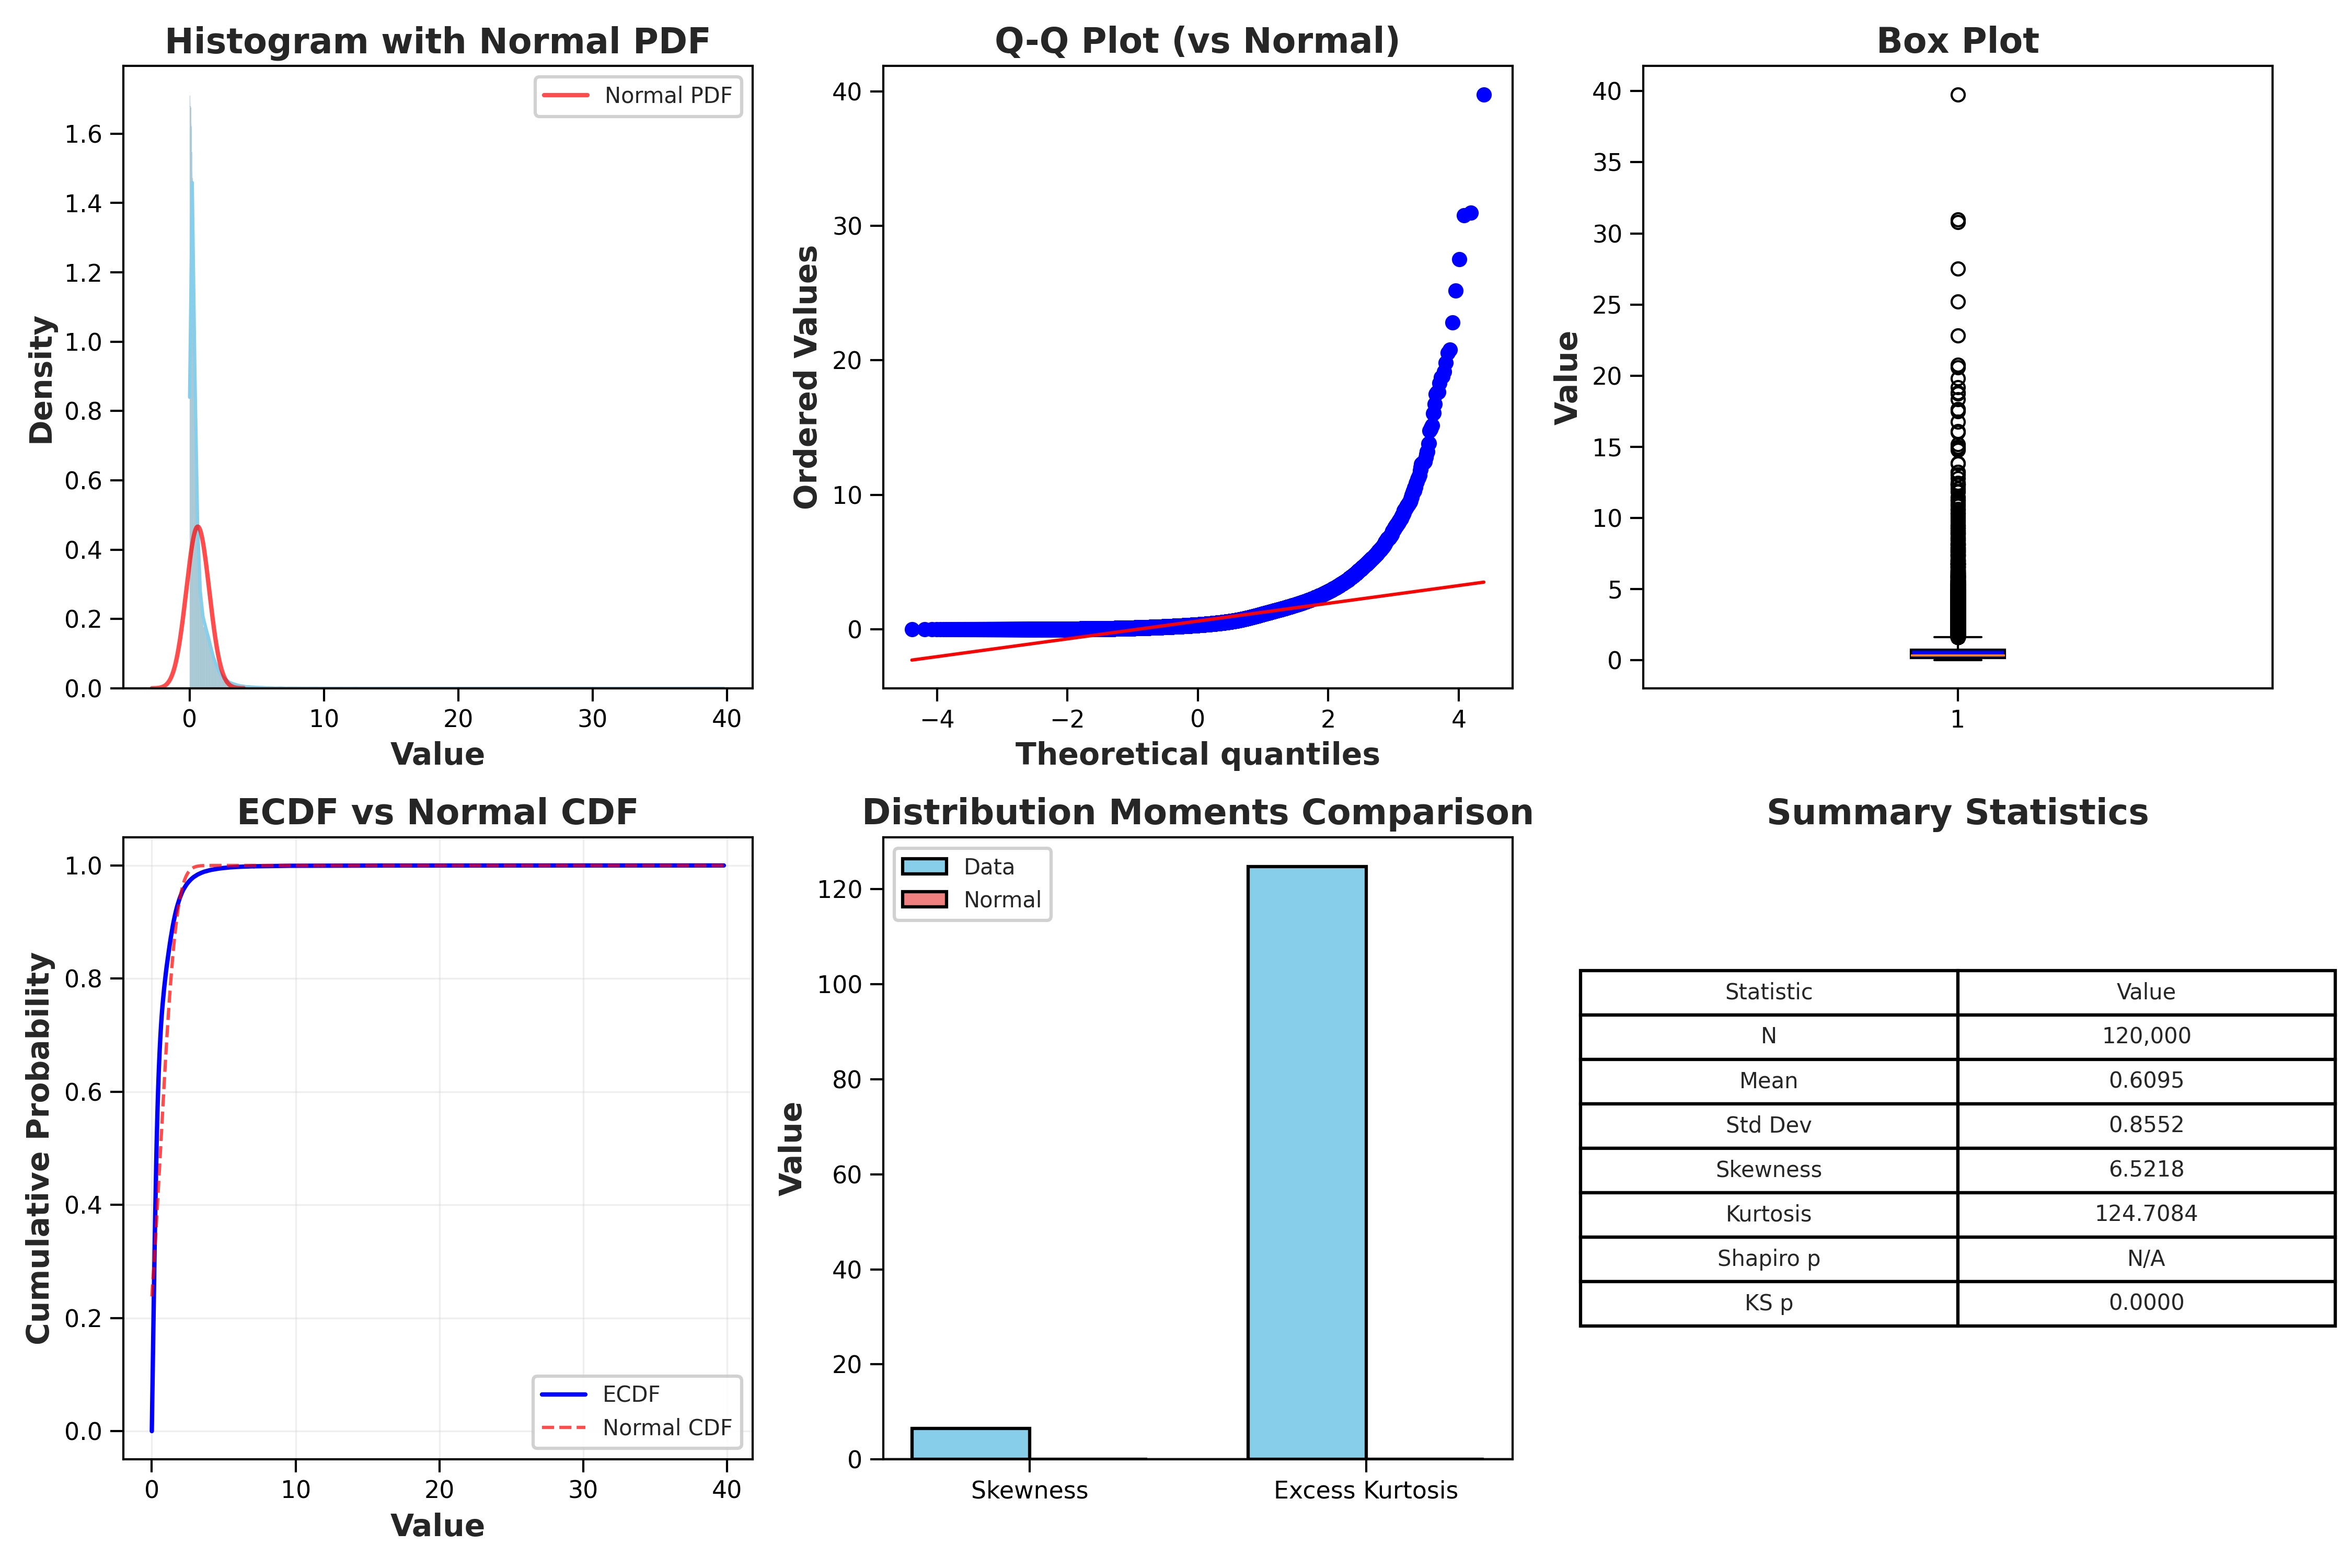
\includegraphics[width=0.48\textwidth]{val_dist_analysis_ape.png}
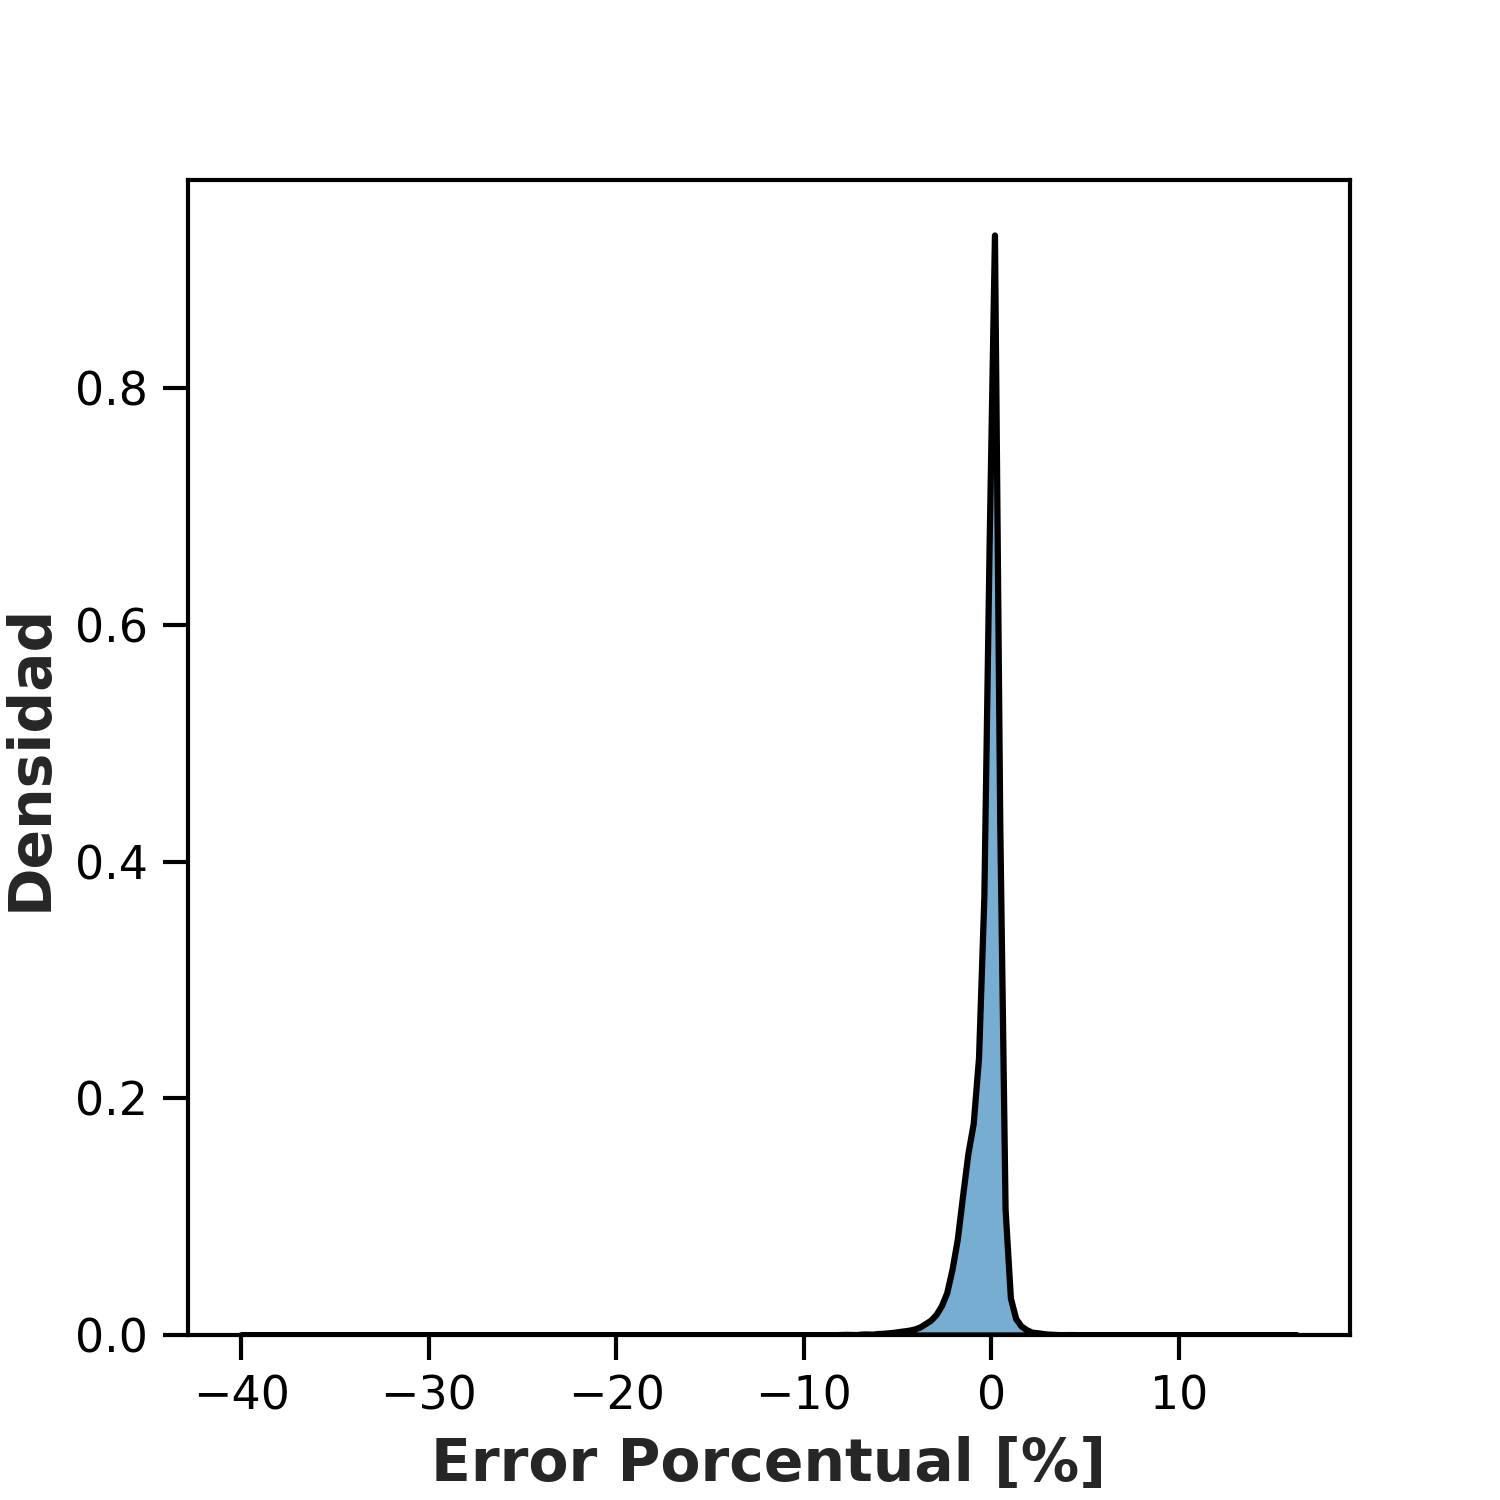
\includegraphics[width=0.48\textwidth]{val_dist_pe.png}
\caption{División Validación: análisis diagnóstico APE (izq.) y distribución PE (der.).}
\label{fig:val-3}
\end{figure}

\begin{figure}[htbp]
\centering
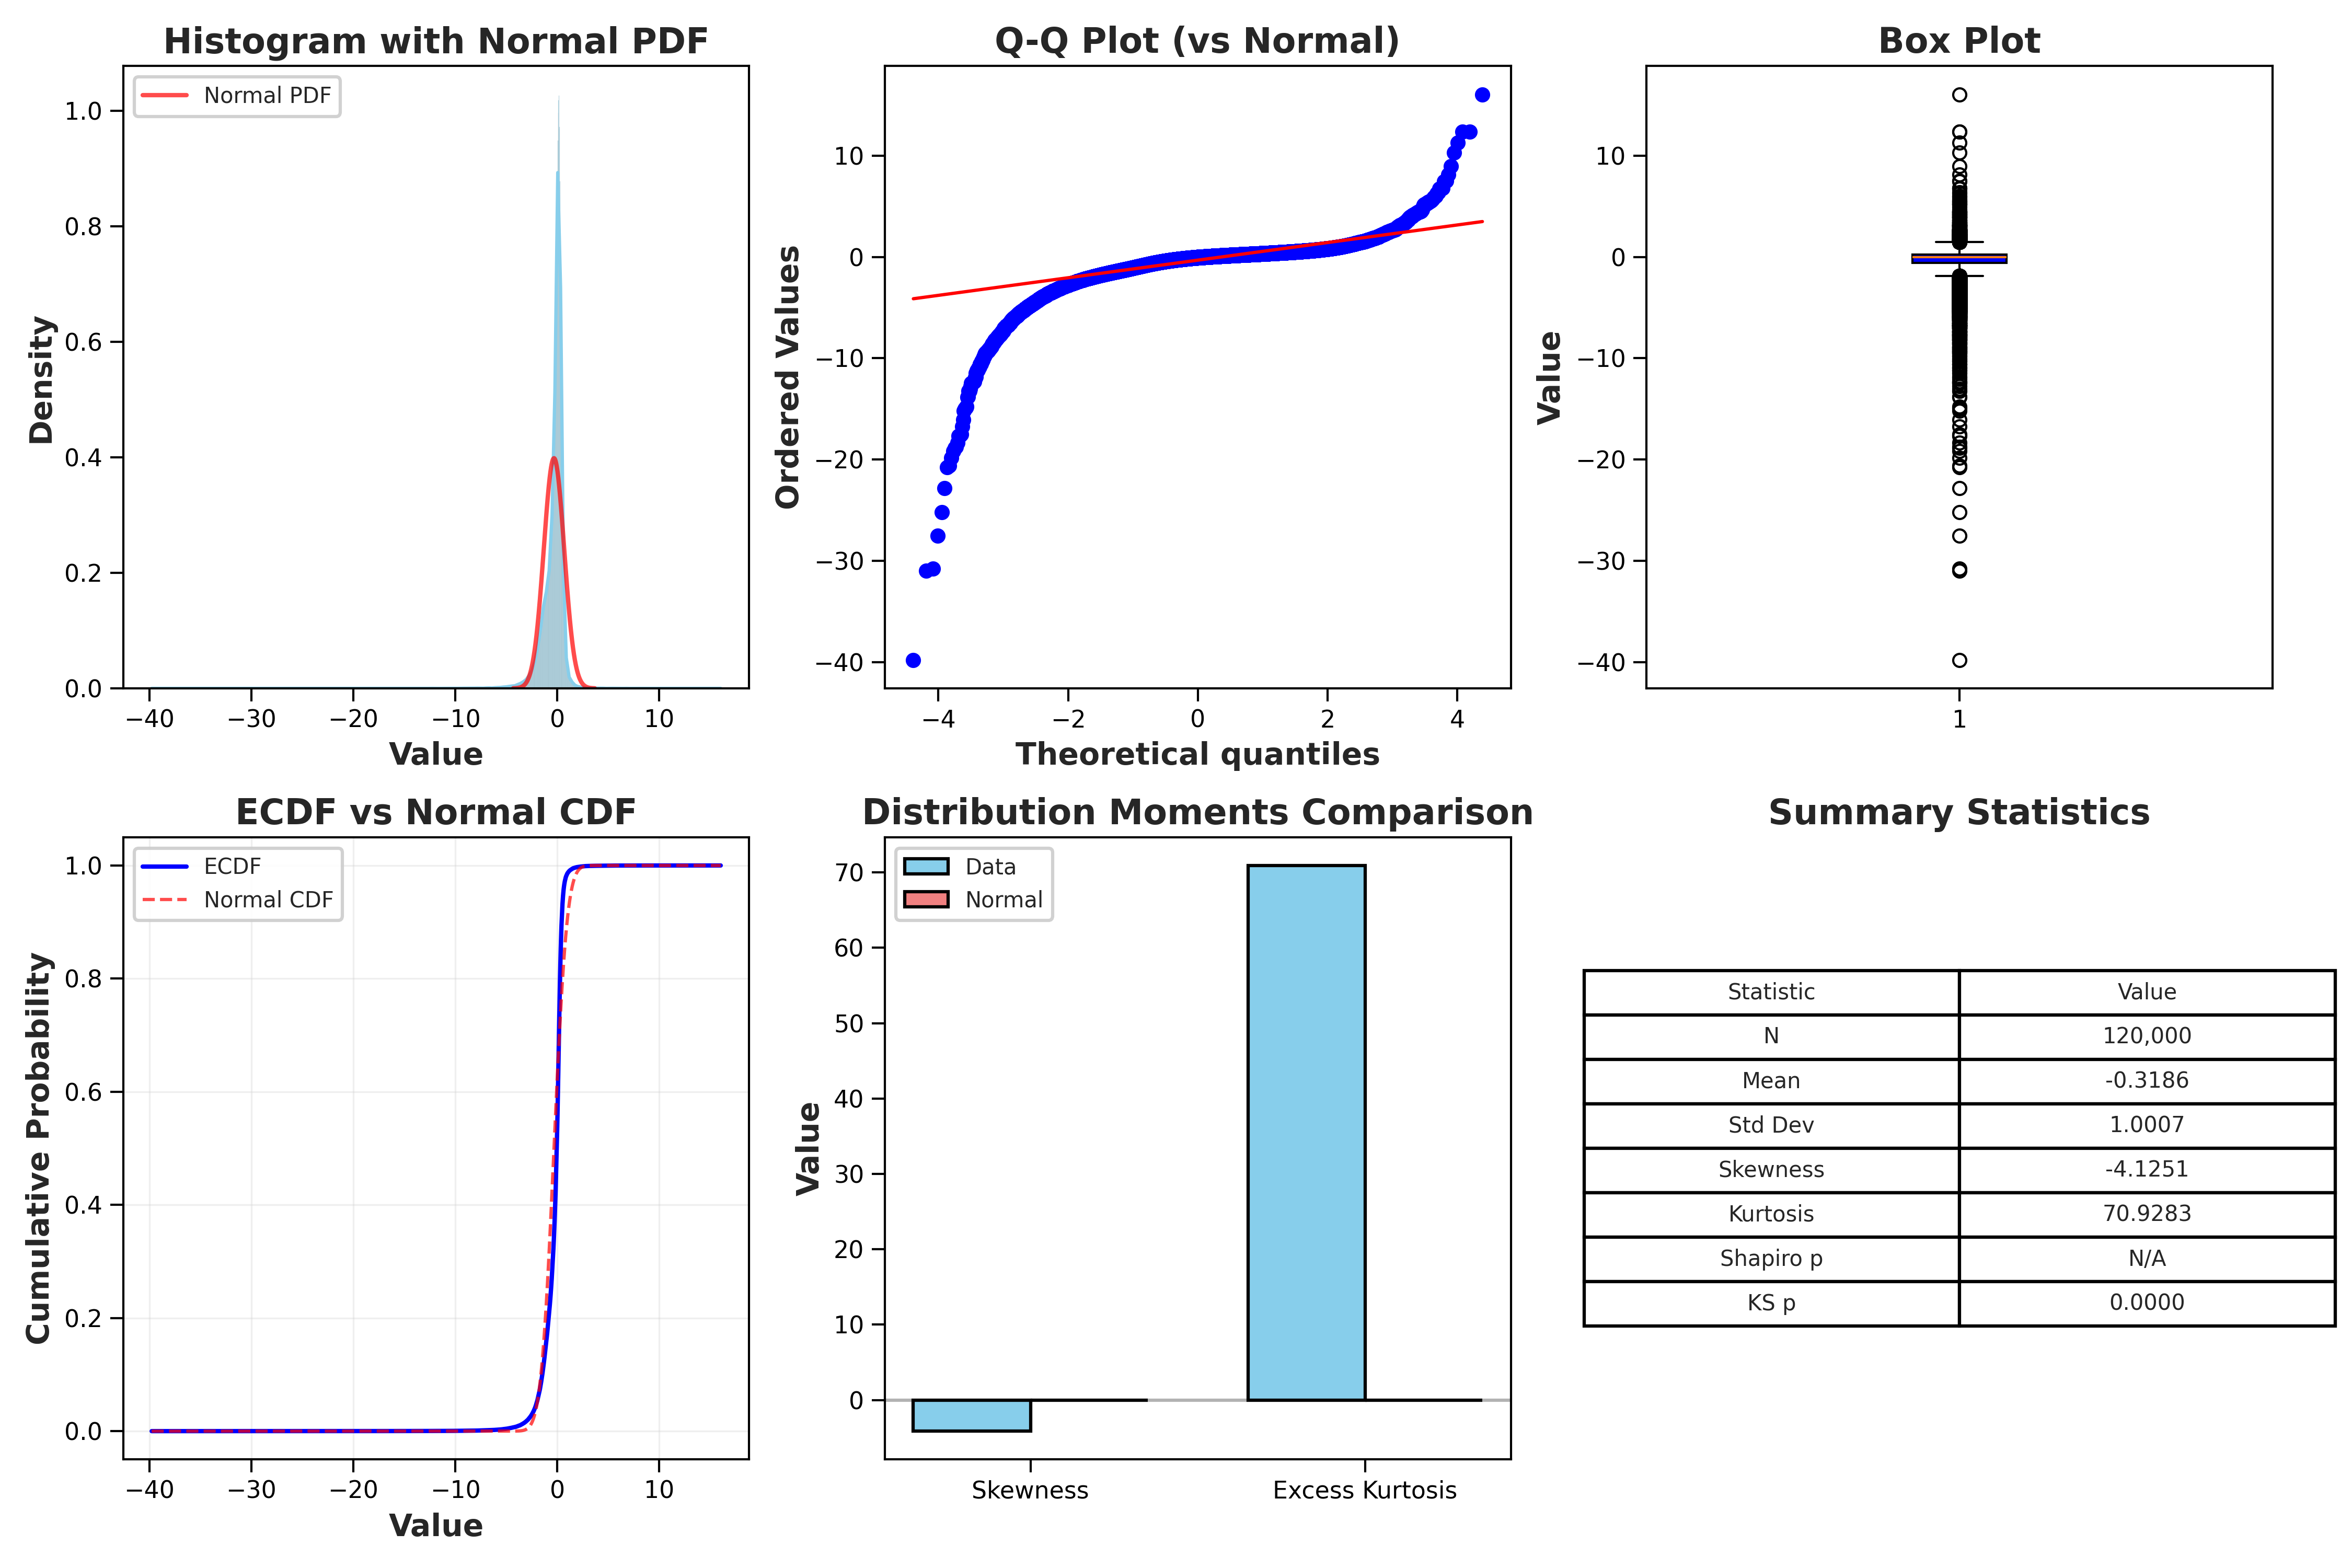
\includegraphics[width=0.7\textwidth]{val_dist_analysis_pe.png}
\caption{División Validación: análisis diagnóstico PE (6 paneles).}
\label{fig:val-4}
\end{figure}

%%%%%%%%%%%%%%%%%%%%%%%%%%%%%%%%%%%%%%%%%%%%%%%%%%%%%%%%%%%%%%
\subsection{División Test ($N = 120{,}000$)}
%%%%%%%%%%%%%%%%%%%%%%%%%%%%%%%%%%%%%%%%%%%%%%%%%%%%%%%%%%%%%%

\subsubsection{Métricas de Error}

\begin{table}[htbp]
\centering
\caption{Métricas de error — División Test.}
\label{tab:test-metrics}
\begin{tabular}{ll}
\hline
Métrica & Valor \\
\hline
MAE  & 2.93~nm \\
MSE  & 15.14~nm$^2$ \\
RMSE & 3.89~nm \\
MAPE & 0.62\% \\
$R^2$ & 0.9999 \\
\hline
\end{tabular}
\end{table}

\subsubsection{Distribución APE (Error Porcentual Absoluto)}

\begin{table}[htbp]
\centering
\caption{Estadísticos de la distribución APE — Test.}
\label{tab:test-ape}
\begin{tabular}{ll}
\hline
Estadístico & Valor \\
\hline
Media                    & 0.6153\% \\
Mediana                  & 0.3280\% \\
Desviación Estándar      & 0.8716\% \\
Máximo APE               & 44.97\% \\
Asimetría (Skewness)     & 7.2378 (la más alta entre divisiones simuladas) \\
Curtosis (Exceso)        & 167.2586 (la de colas más pesadas entre simuladas) \\
Outliers (IQR)           & 10,243 (8.54\%) \\
\hline
\end{tabular}
\end{table}

\textbf{Normalidad:} Rechazada por todas las pruebas (KS $D = 0.2401$, AD $A^2 = 11{,}389.35$, JB $= 1.41 \times 10^8$, todos $p \approx 0$).

\subsubsection{Distribución PE (Error Porcentual)}

\begin{table}[htbp]
\centering
\caption{Estadísticos de la distribución PE — Test.}
\label{tab:test-pe}
\begin{tabular}{ll}
\hline
Estadístico & Valor \\
\hline
Media                    & $-0.3210\%$ \\
Mediana                  & $-0.0468\%$ \\
Desviación Estándar      & 1.0175\% \\
Asimetría (Skewness)     & $-4.2738$ \\
Curtosis (Exceso)        & 95.4401 \\
Outliers (IQR)           & 7,774 (6.48\%) \\
\hline
\end{tabular}
\end{table}

\subsubsection{Figuras — División Test}

\begin{figure}[htbp]
\centering
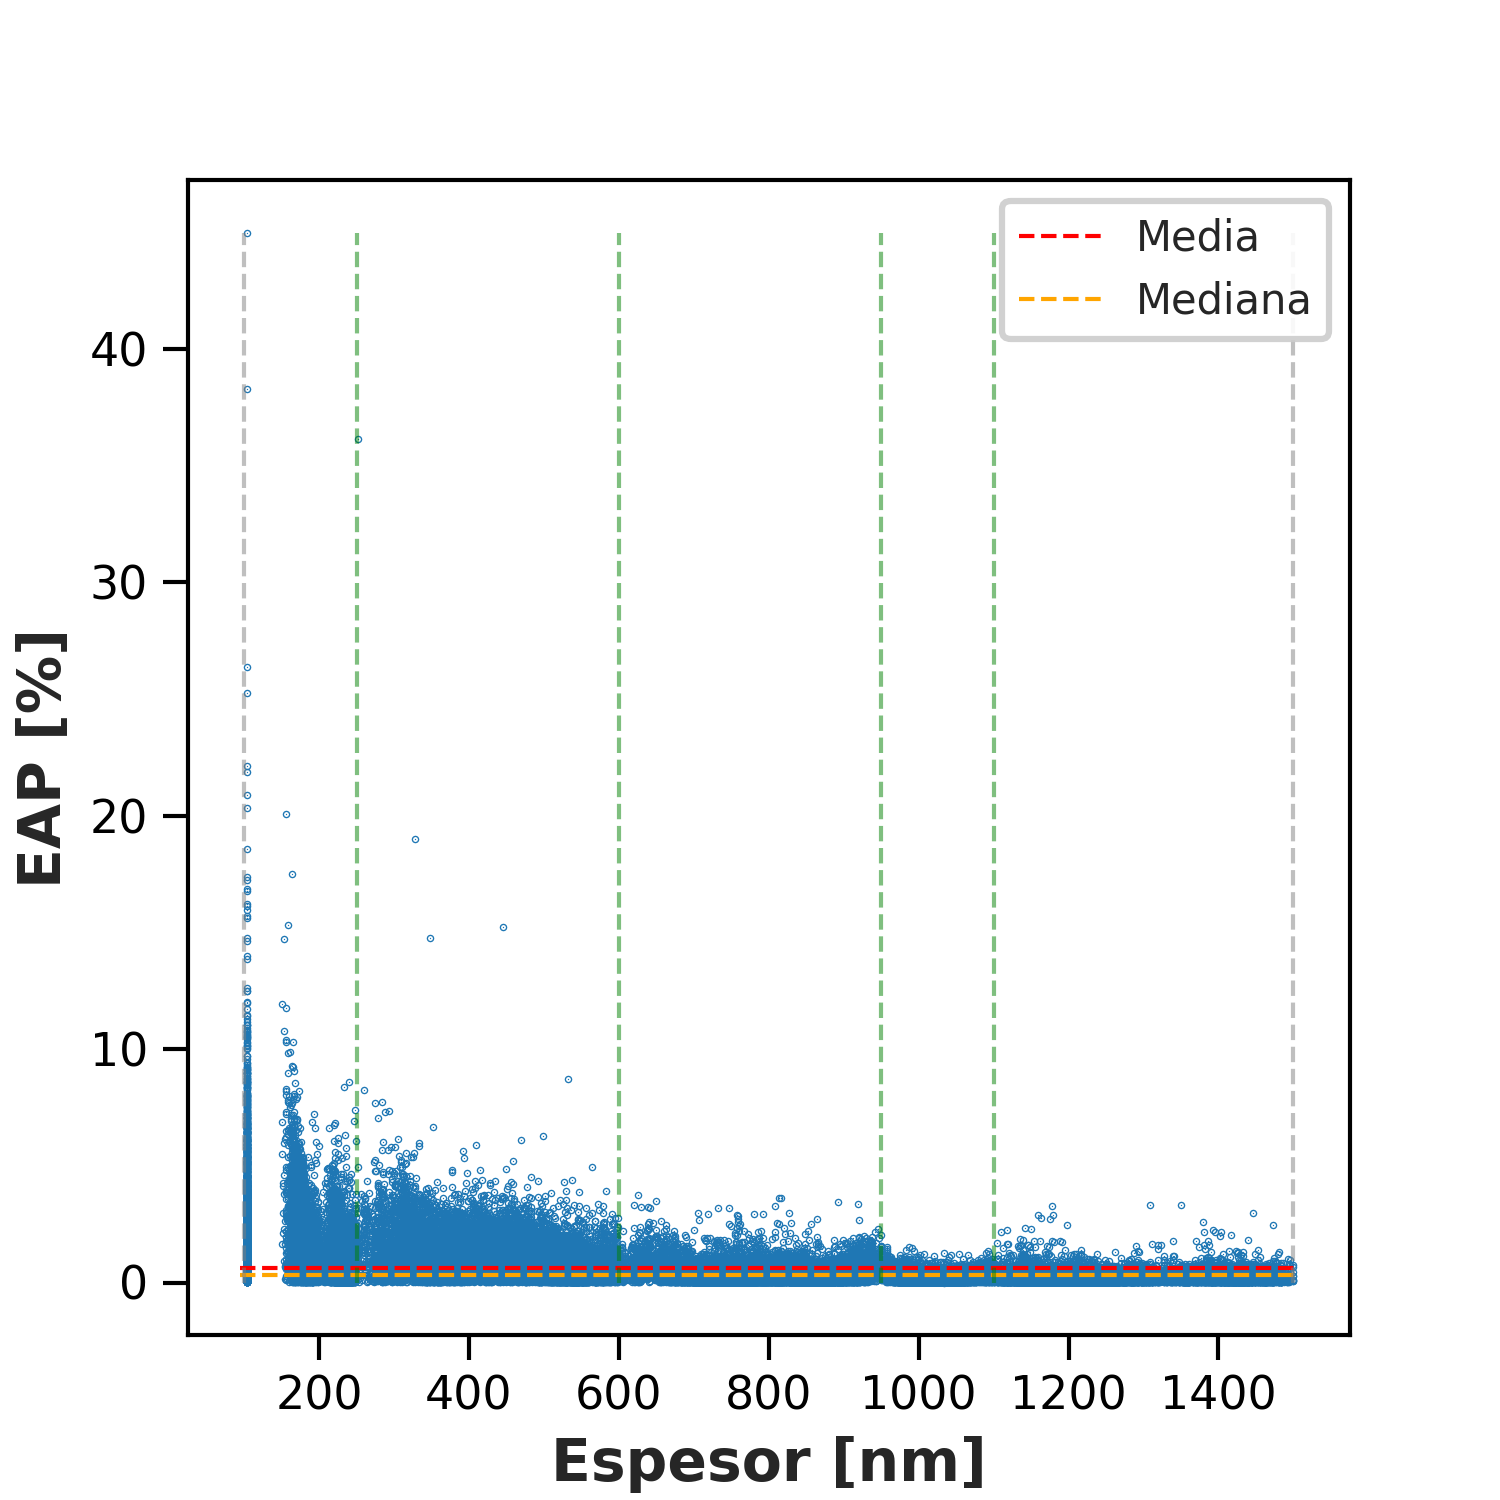
\includegraphics[width=0.48\textwidth]{test_error.png}
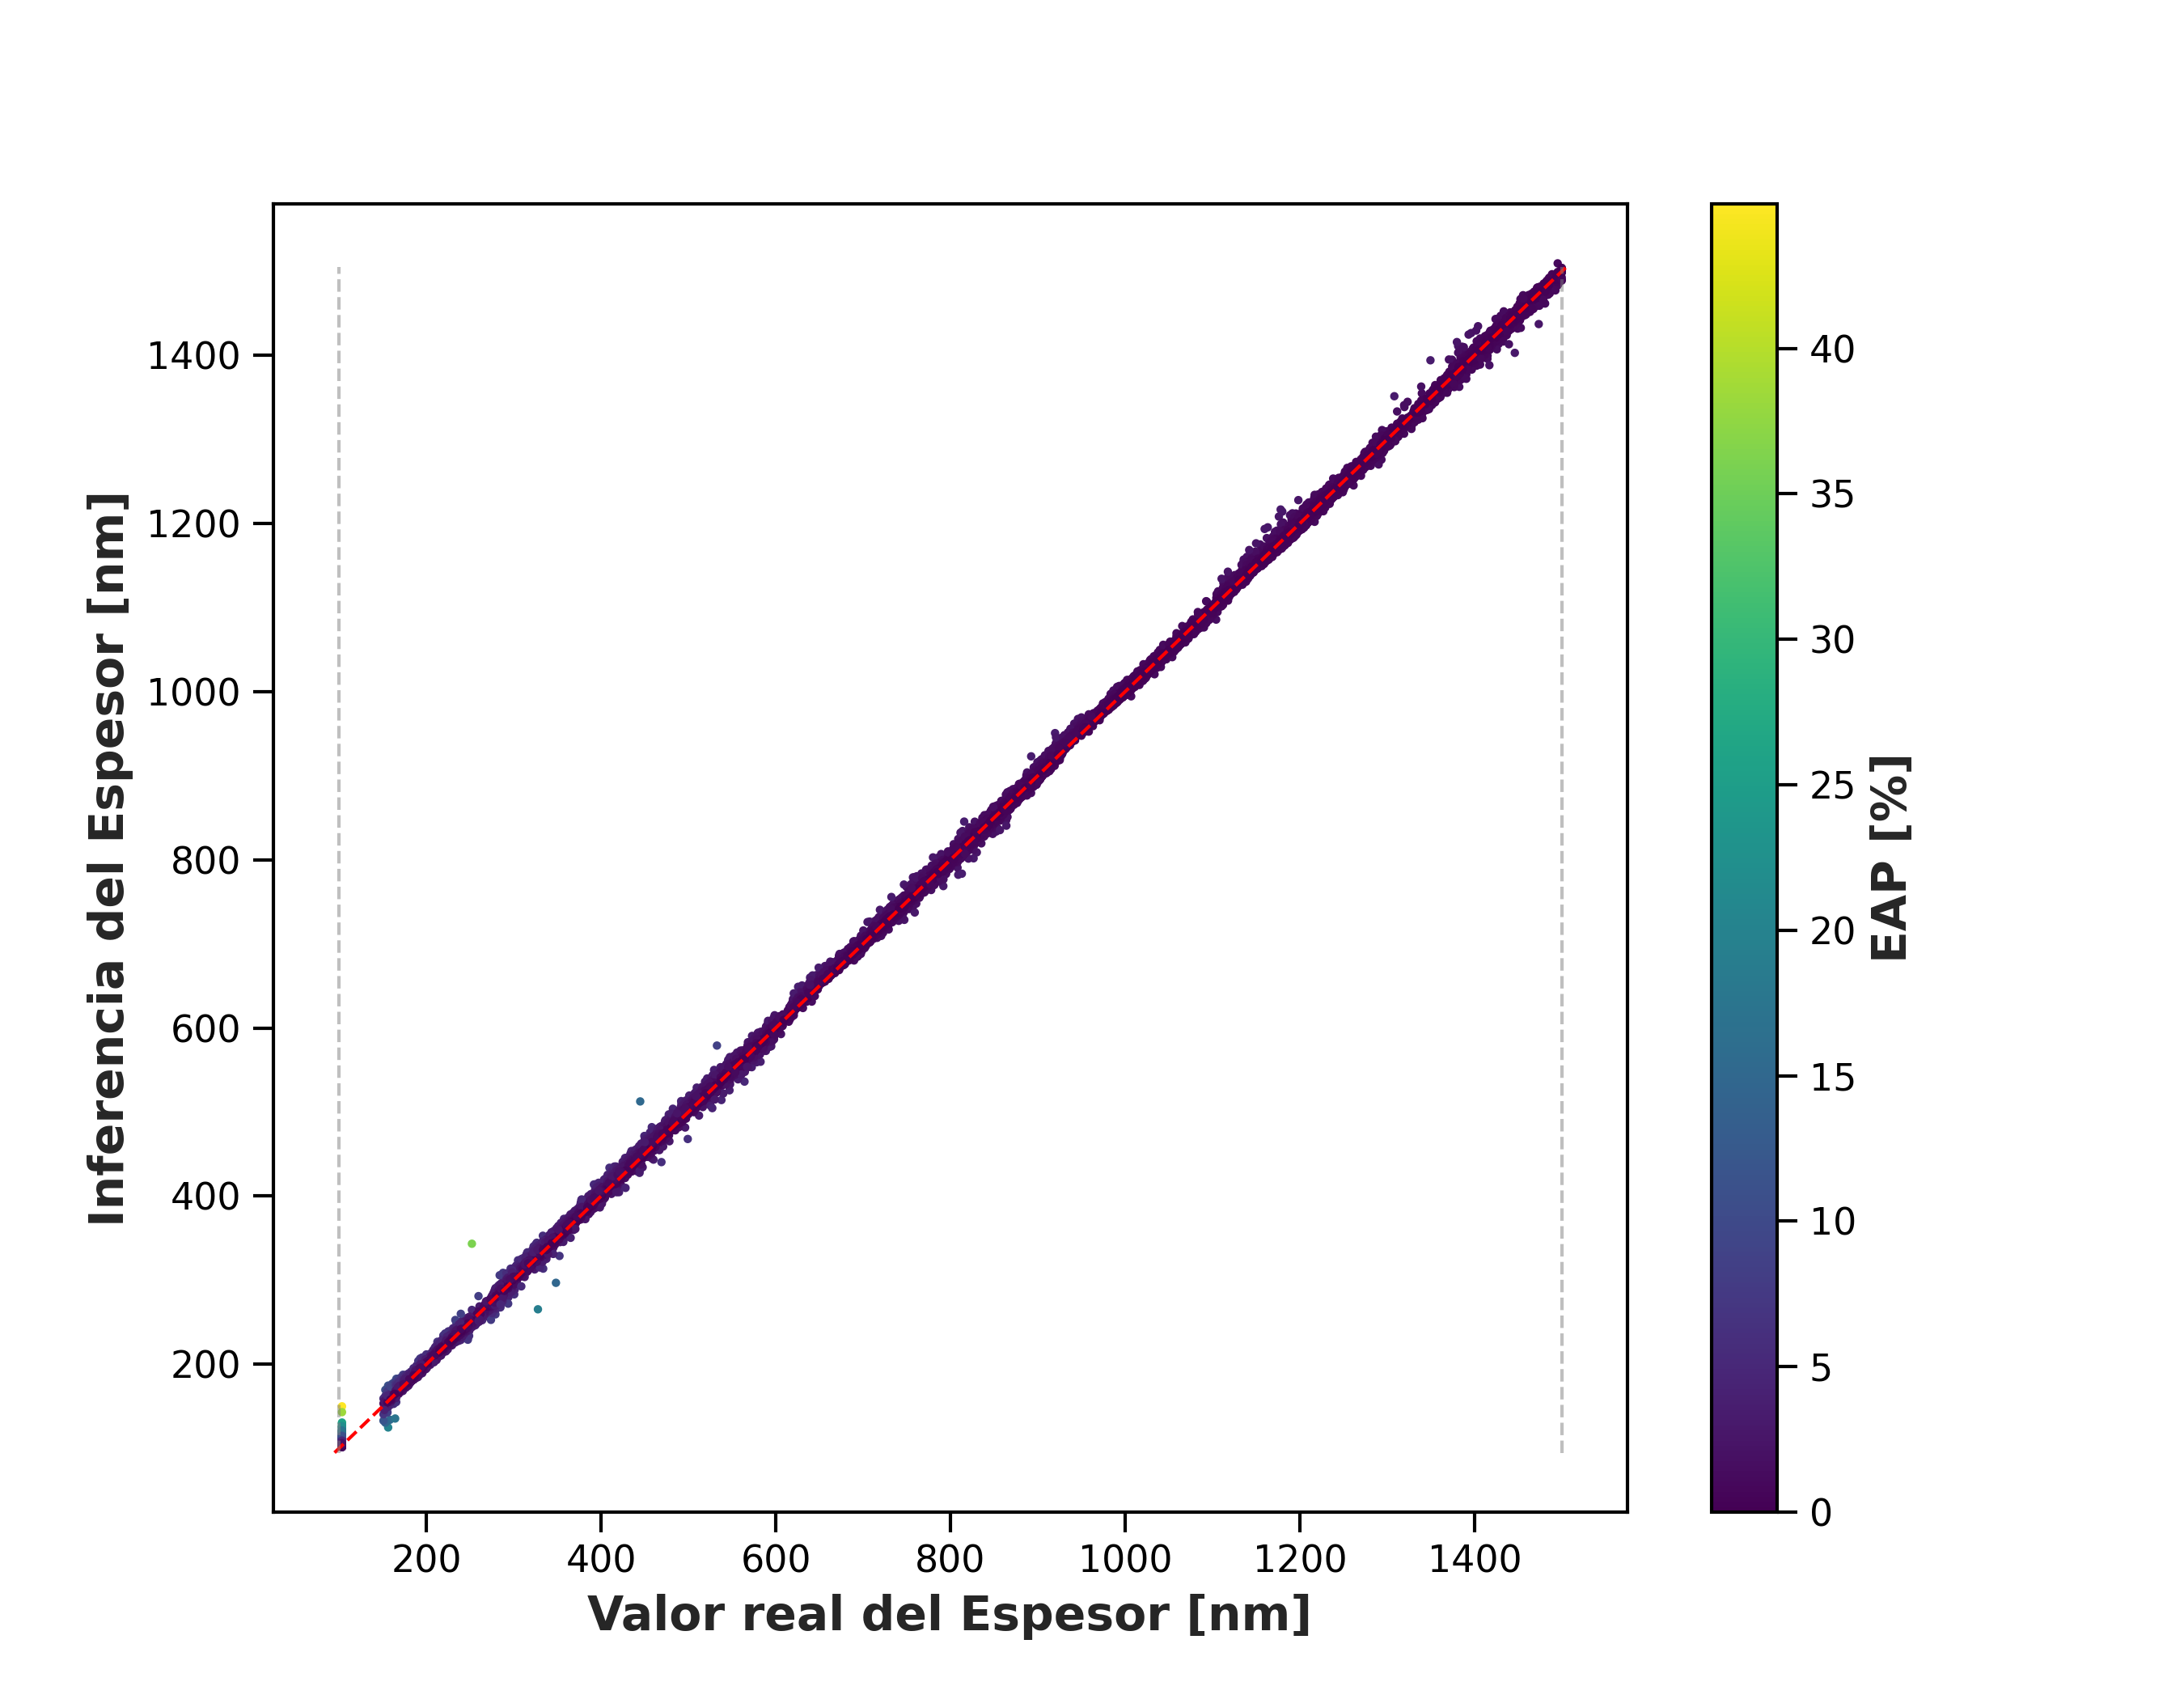
\includegraphics[width=0.48\textwidth]{test_comparsion_true_preds.png}
\caption{División Test: error de predicción (izq.) y comparación real vs predicho (der.).}
\label{fig:test-1}
\end{figure}

\begin{figure}[htbp]
\centering
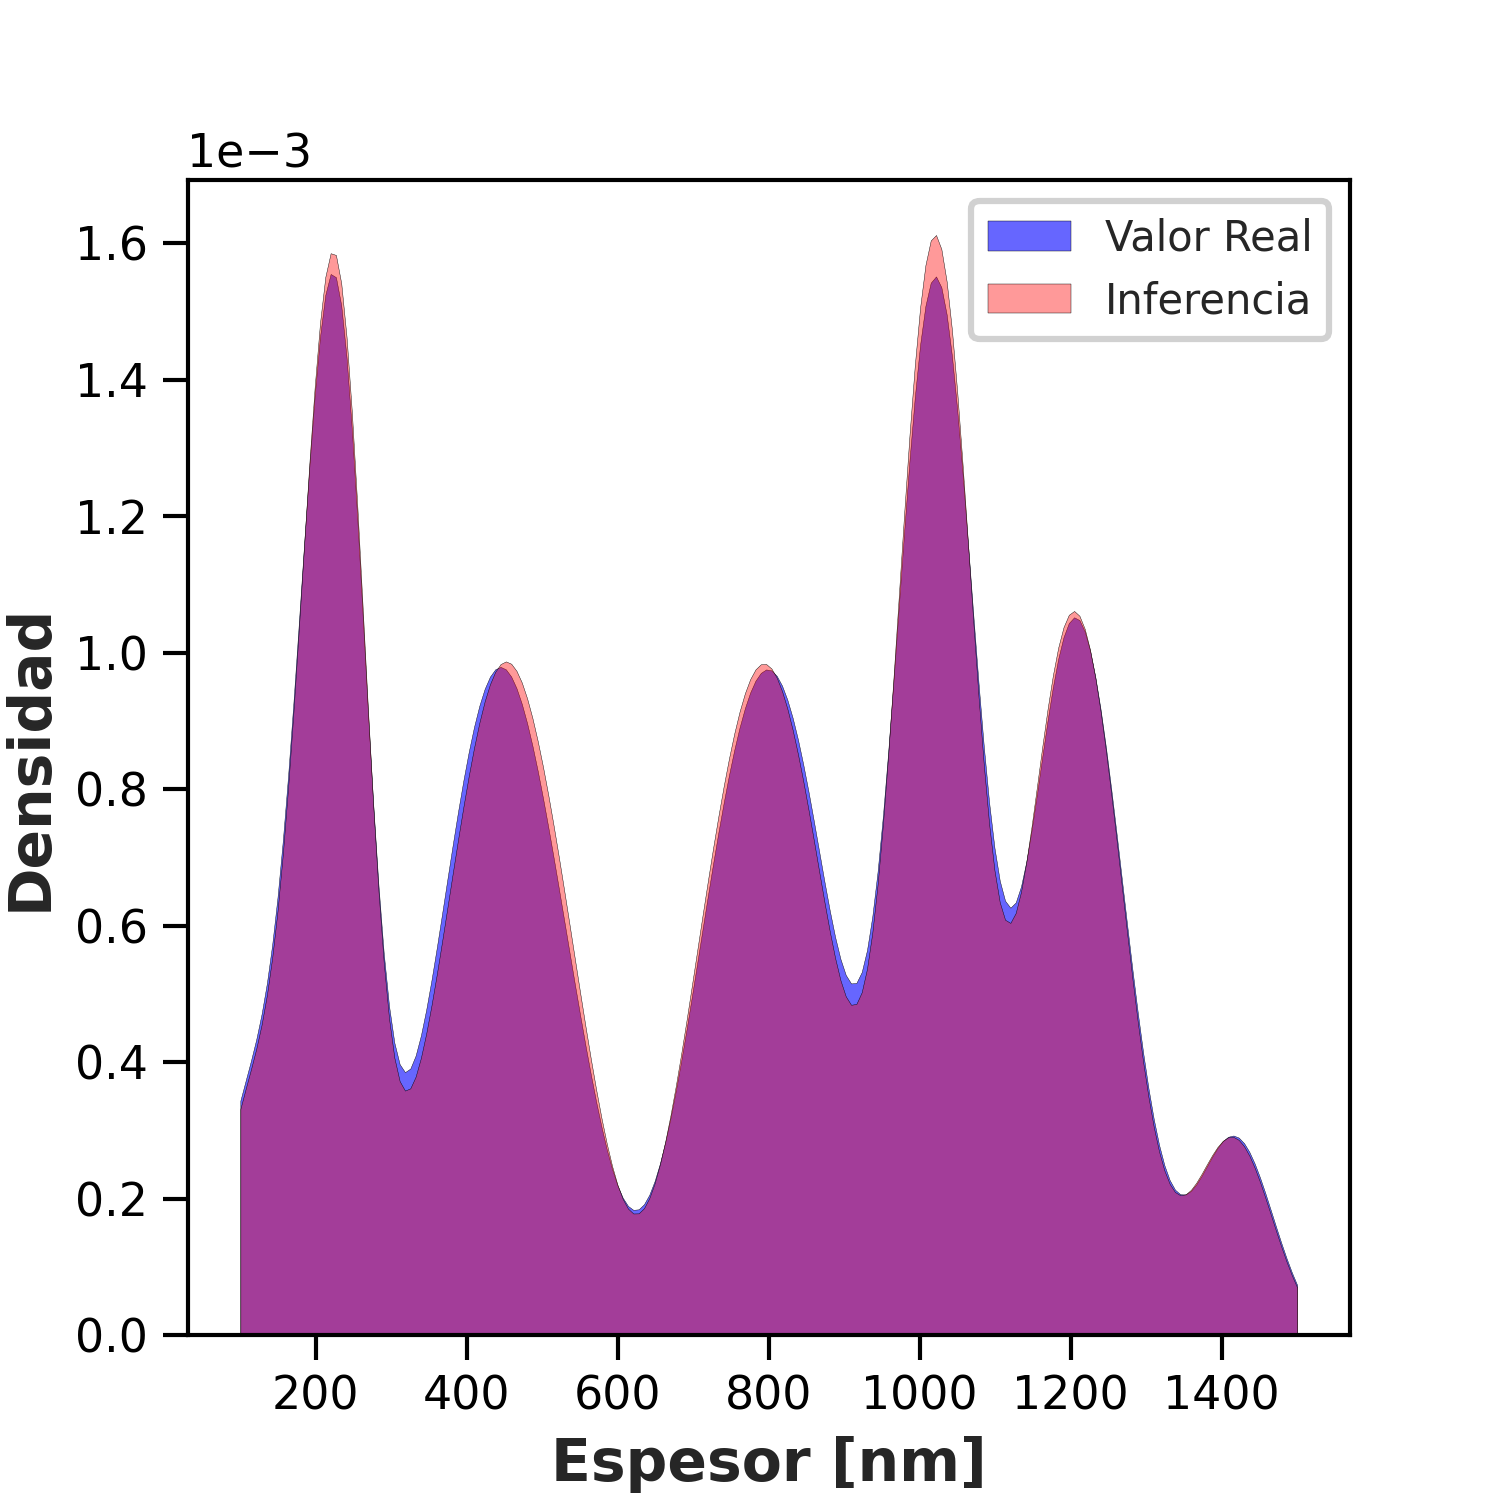
\includegraphics[width=0.48\textwidth]{test_two_dist.png}
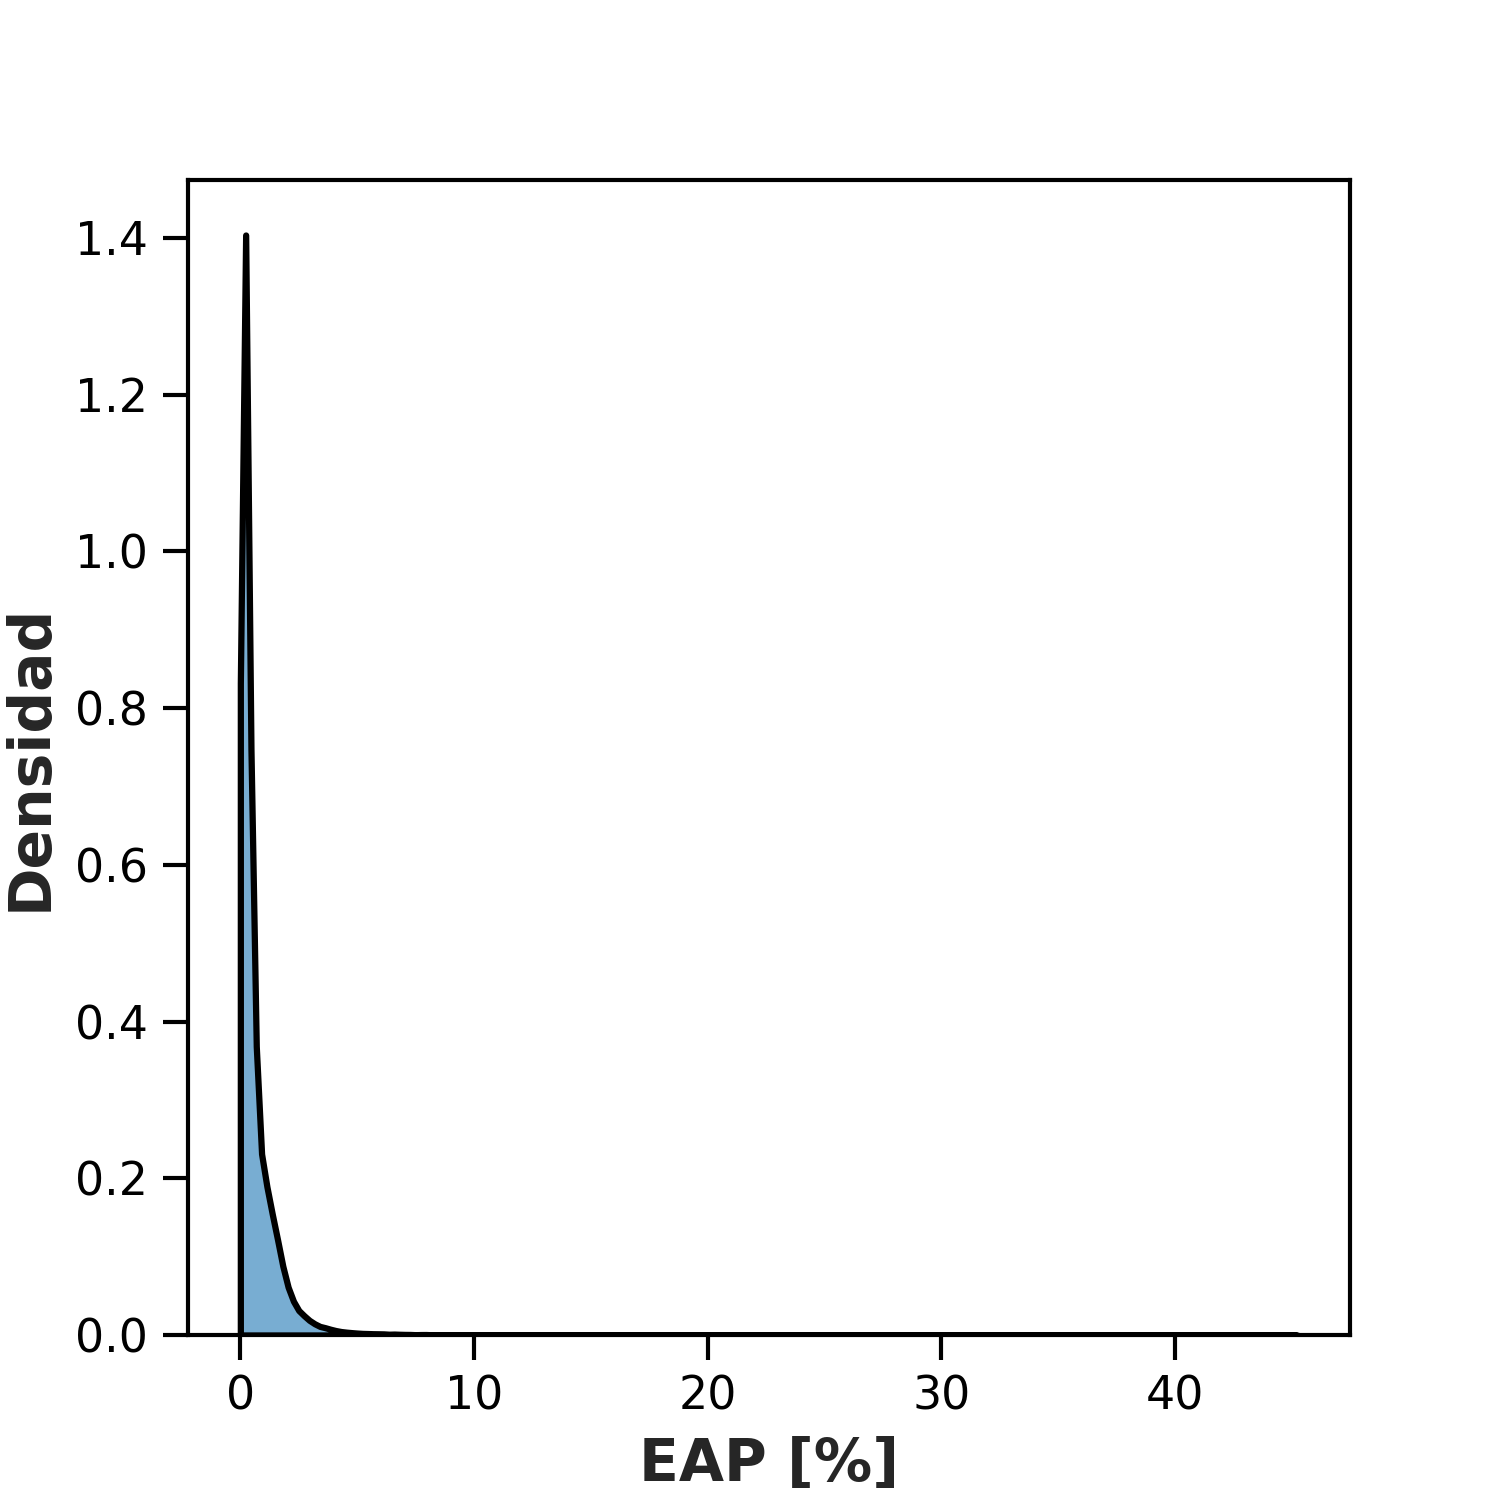
\includegraphics[width=0.48\textwidth]{test_dist_ape.png}
\caption{División Test: distribuciones superpuestas (izq.) y distribución APE (der.).}
\label{fig:test-2}
\end{figure}

\begin{figure}[htbp]
\centering
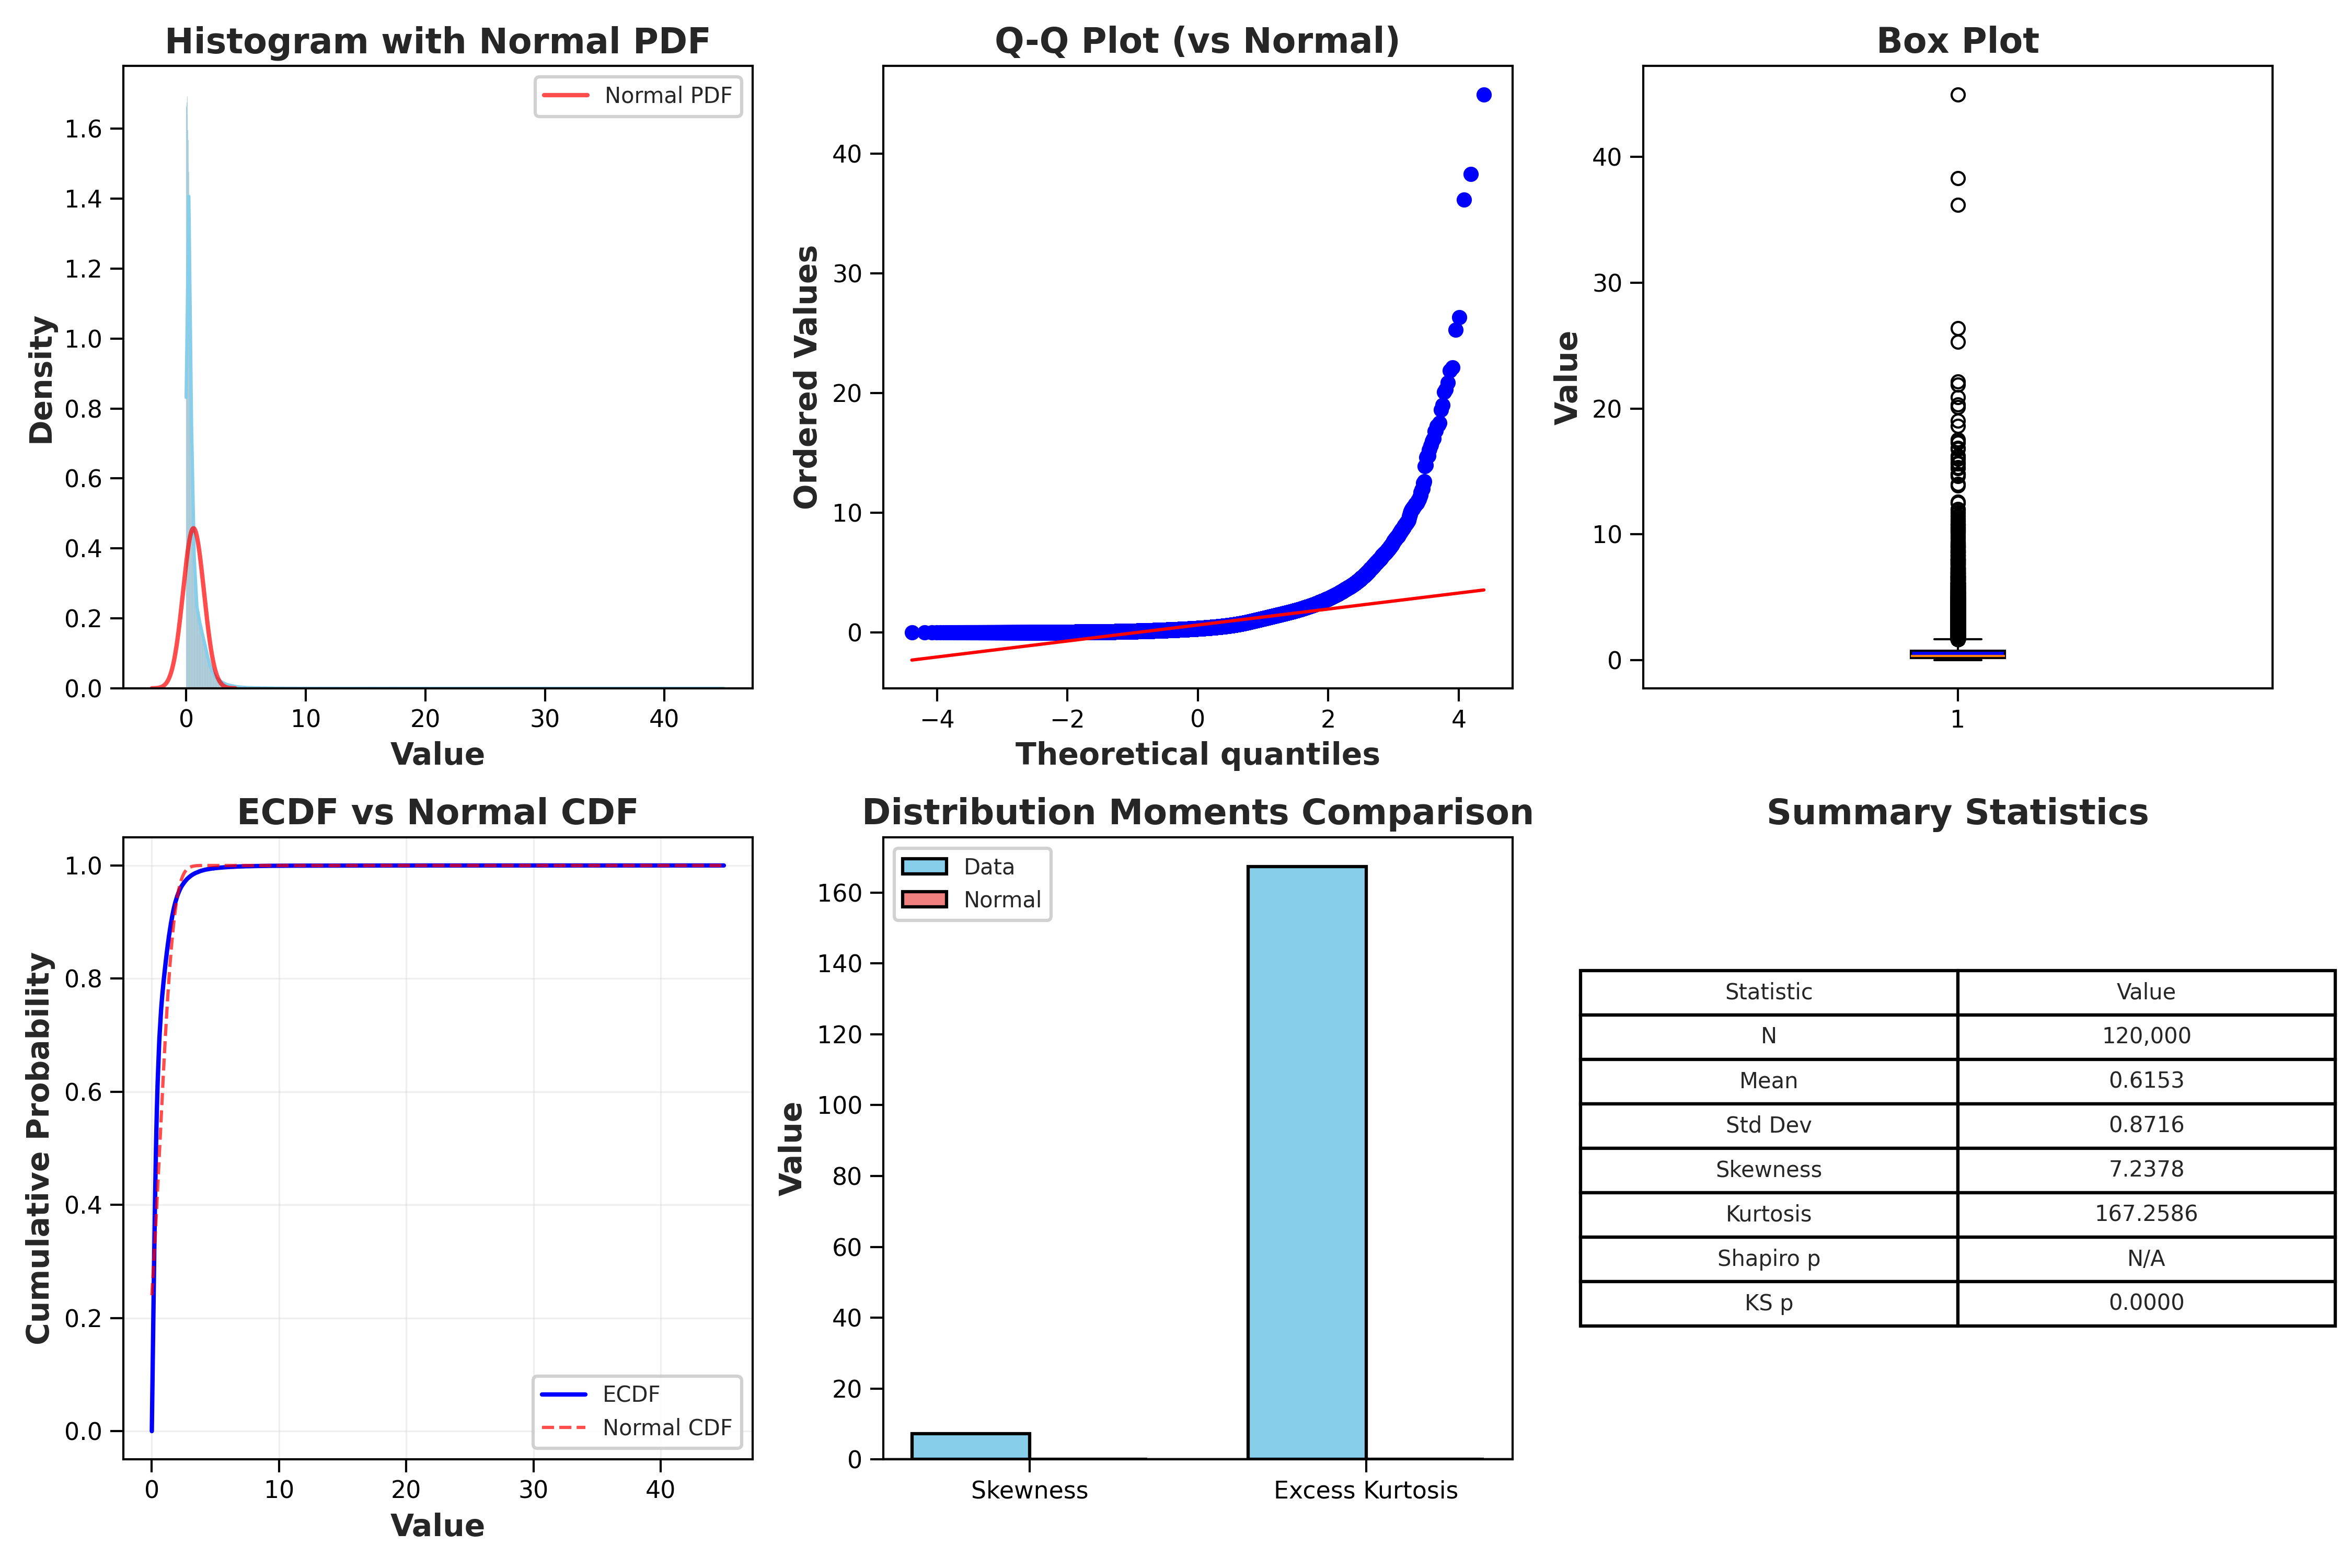
\includegraphics[width=0.48\textwidth]{test_dist_analysis_ape.png}
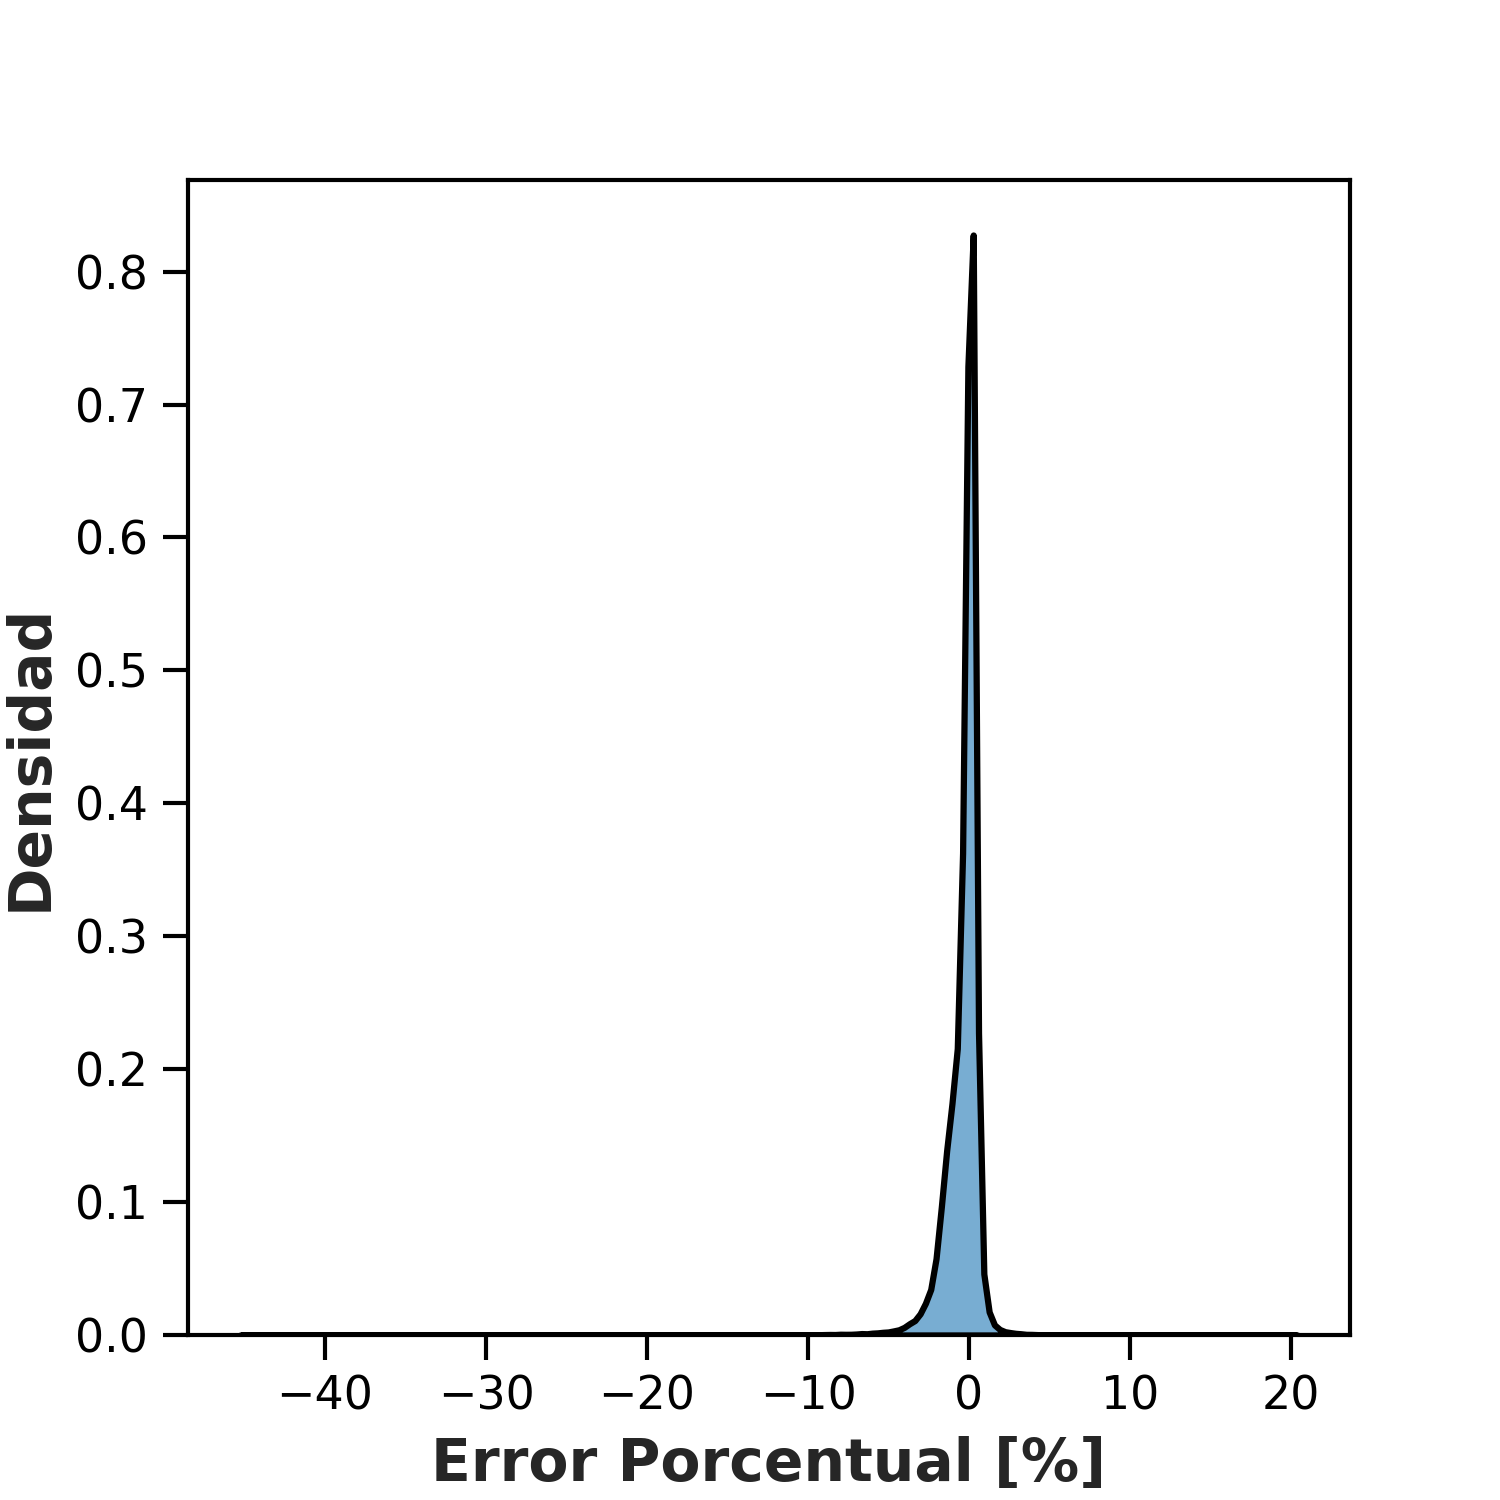
\includegraphics[width=0.48\textwidth]{test_dist_pe.png}
\caption{División Test: análisis diagnóstico APE (izq.) y distribución PE (der.).}
\label{fig:test-3}
\end{figure}

\begin{figure}[htbp]
\centering
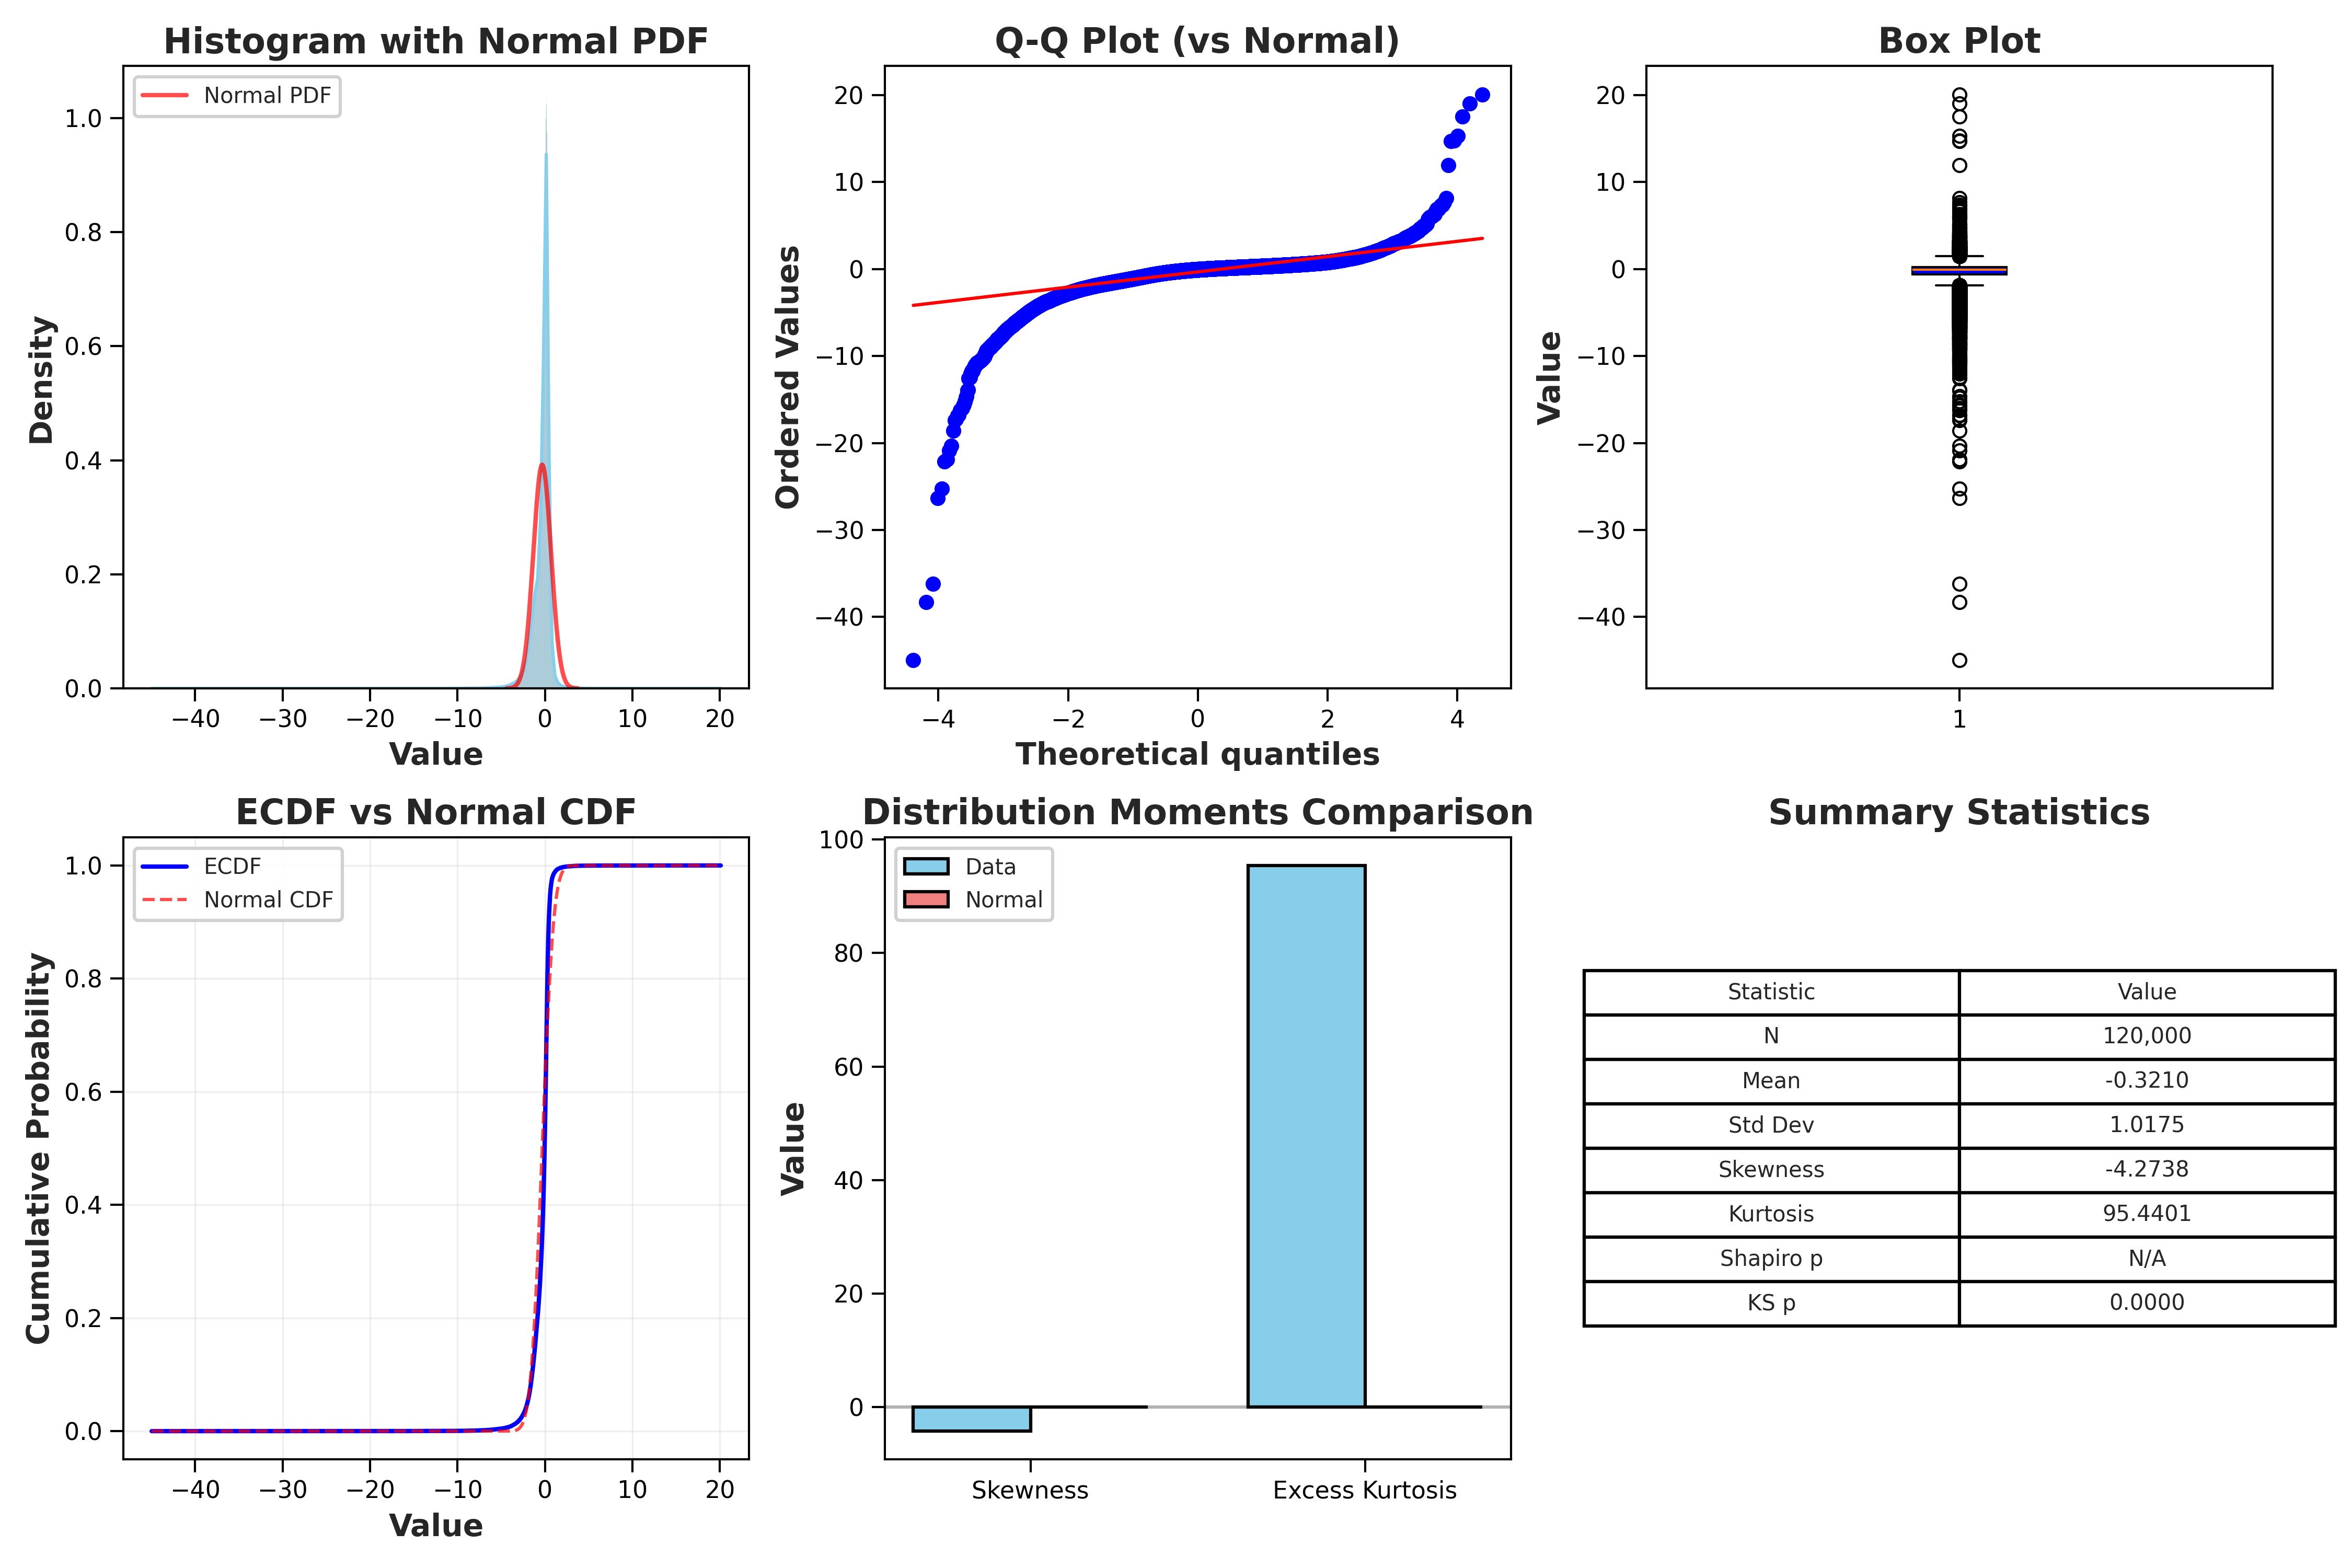
\includegraphics[width=0.7\textwidth]{test_dist_analysis_pe.png}
\caption{División Test: análisis diagnóstico PE (6 paneles).}
\label{fig:test-4}
\end{figure}

%%%%%%%%%%%%%%%%%%%%%%%%%%%%%%%%%%%%%%%%%%%%%%%%%%%%%%%%%%%%%%
\subsection{Datos Experimentales 145 ($N = 145$)}
%%%%%%%%%%%%%%%%%%%%%%%%%%%%%%%%%%%%%%%%%%%%%%%%%%%%%%%%%%%%%%

\subsubsection{Métricas de Error}

\begin{table}[htbp]
\centering
\caption{Métricas de error — Muestras Experimentales 145.}
\label{tab:exp145-metrics}
\begin{tabular}{ll}
\hline
Métrica & Valor \\
\hline
MAE  & 58.77~nm \\
MSE  & 7,029.82~nm$^2$ \\
RMSE & 83.84~nm \\
MAPE & 7.38\% \\
$R^2$ & 0.9385 \\
\hline
\end{tabular}
\end{table}

\subsubsection{Distribución APE (Error Porcentual Absoluto)}

\begin{table}[htbp]
\centering
\caption{Estadísticos de la distribución APE — Experimental 145.}
\label{tab:exp145-ape}
\begin{tabular}{ll}
\hline
Estadístico & Valor \\
\hline
Media                        & 7.3797\% \\
Mediana                      & 6.4231\% \\
Desviación Estándar          & 5.8508\% \\
Mínimo                       & 0.0049\% \\
Máximo                       & 27.6275\% \\
Asimetría (Skewness)         & 0.8061 (moderadamente sesgada, derecha) \\
Curtosis (Exceso)            & 0.1797 (mesocúrtica — cercana a normal) \\
Outliers (IQR)               & 1 (0.69\%) \\
Coeficiente de Variación     & 0.7928 \\
\hline
\end{tabular}
\end{table}

\textbf{Pruebas de Normalidad para APE:}
\begin{itemize}
\item Shapiro-Wilk: $W = 0.9286$, $p = 1 \times 10^{-6}$ $\rightarrow$ Rechazada.
\item Kolmogorov-Smirnov: $D = 0.1135$, $p = 0.044$ $\rightarrow$ Límite.
\item Anderson-Darling: $A^2 = 2.7328 > 0.7670$ $\rightarrow$ Rechazada al 5\%.
\item Jarque-Bera: $\text{JB} = 15.49$, $p = 0.0004$ $\rightarrow$ Rechazada.
\end{itemize}

\subsubsection{Distribución PE (Error Porcentual) — \texorpdfstring{¡Normal!}{¡Normal!}}

\begin{table}[htbp]
\centering
\caption{Estadísticos de la distribución PE — Experimental 145.}
\label{tab:exp145-pe}
\begin{tabular}{ll}
\hline
Estadístico & Valor \\
\hline
Media                        & $-1.7618\%$ \\
Mediana                      & $-1.0253\%$ \\
Desviación Estándar          & 9.2706\% \\
Asimetría (Skewness)         & $-0.0321$ (aproximadamente simétrica) \\
Curtosis (Exceso)            & $-0.1377$ (mesocúrtica) \\
Outliers (IQR)               & 0 (0.00\%) \\
\hline
\end{tabular}
\end{table}

\textbf{PRUEBAS DE NORMALIDAD — ¡NO RECHAZADA POR NINGUNA!}
\begin{itemize}
\item \textbf{Shapiro-Wilk:} $W = 0.9941$, $p = 0.816$ $\rightarrow$ No se rechaza normalidad.
\item \textbf{Kolmogorov-Smirnov:} $D = 0.0720$, $p = 0.421$ $\rightarrow$ No se rechaza.
\item \textbf{Anderson-Darling:} $A^2 = 0.4087 < 0.7670$ $\rightarrow$ No se rechaza al 5\%.
\item \textbf{Jarque-Bera:} $\text{JB} = 0.2074$, $p = 0.902$ $\rightarrow$ No se rechaza.
\end{itemize}

El hecho de que el PE en el conjunto experimental tenga una distribución aproximadamente normal es notable: sugiere que los errores del modelo en datos del mundo real, aunque de mayor magnitud, se comportan como \textbf{ruido Gaussiano no sesgado}. La media negativa del PE ($-1.76\%$) indica una pequeña tendencia sistemática a \textbf{sub-predecir} el espesor en las 145 muestras experimentales.

\subsubsection{Figuras — Datos Experimentales 145}

\begin{figure}[htbp]
\centering
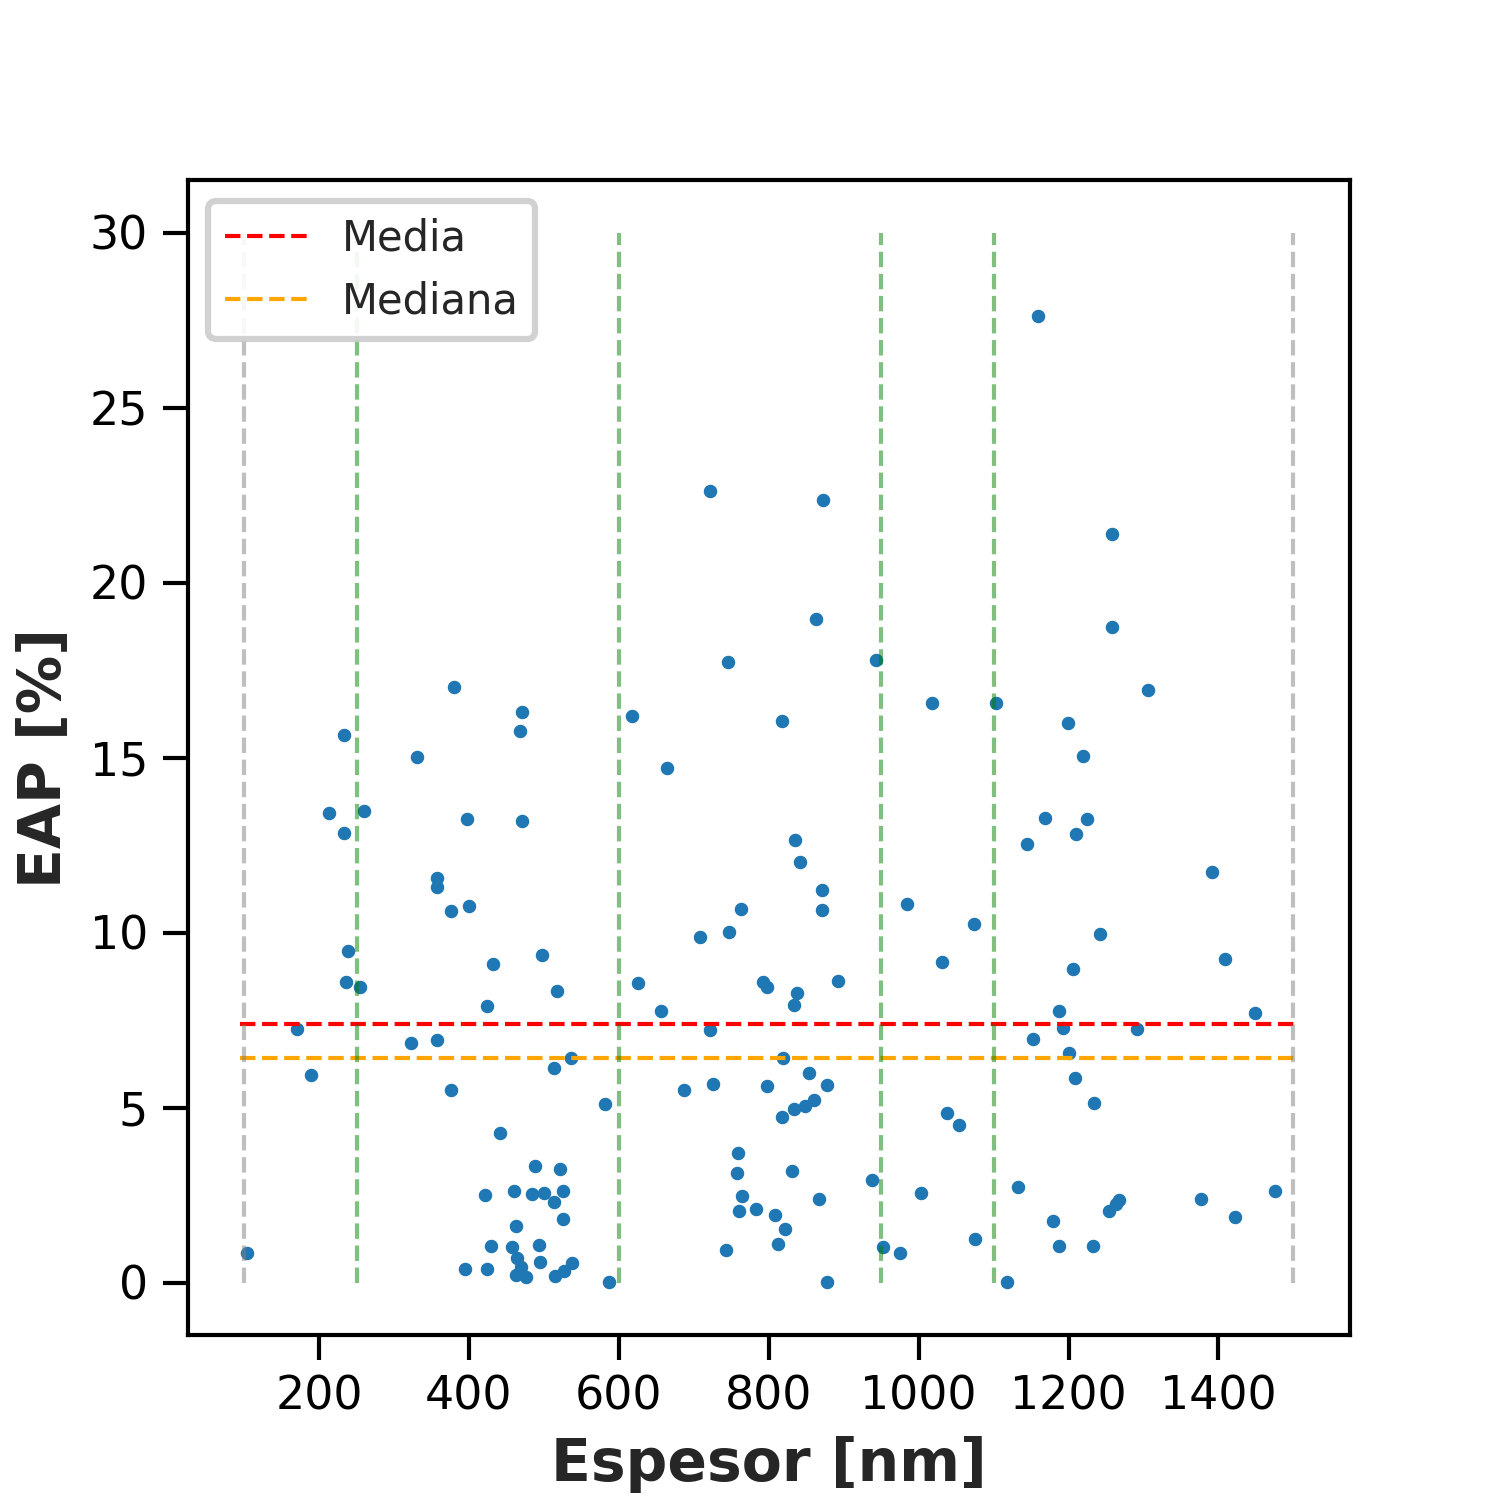
\includegraphics[width=0.48\textwidth]{145_error.png}
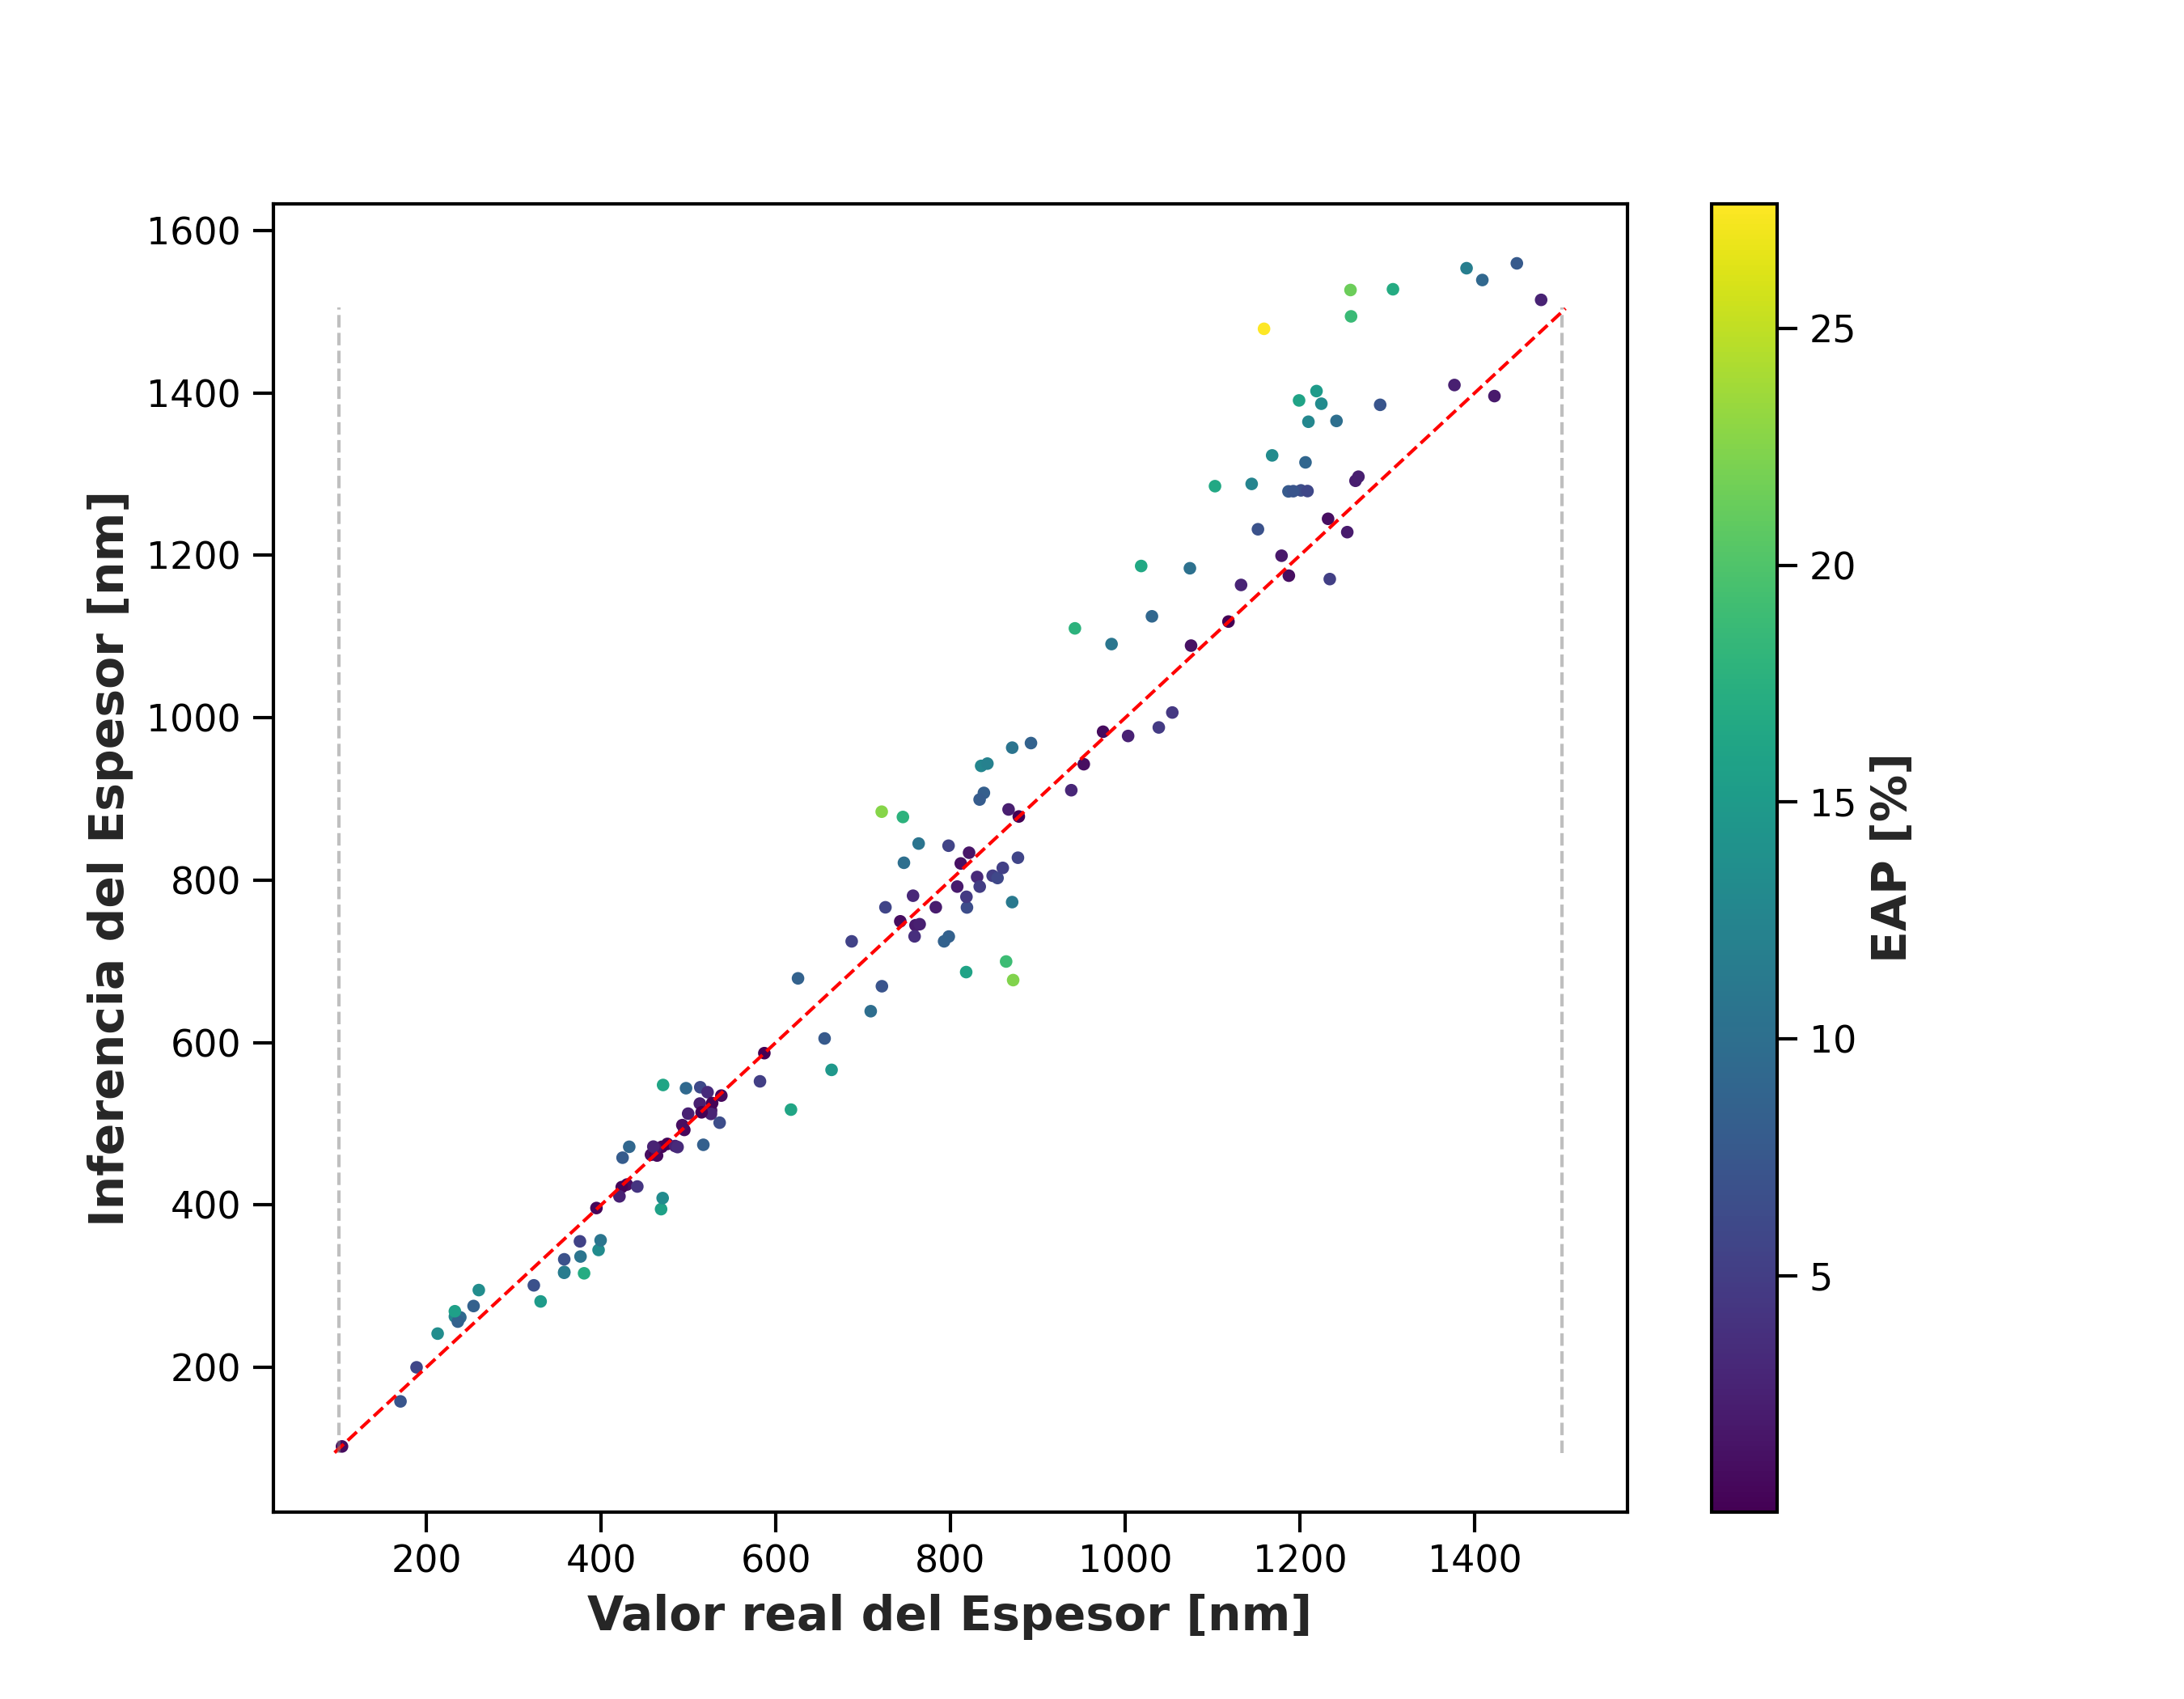
\includegraphics[width=0.48\textwidth]{145_comparsion_true_preds.png}
\caption{Muestras experimentales 145: error de predicción (izq.) y comparación real vs predicho (der.).}
\label{fig:145-1}
\end{figure}

\begin{figure}[htbp]
\centering
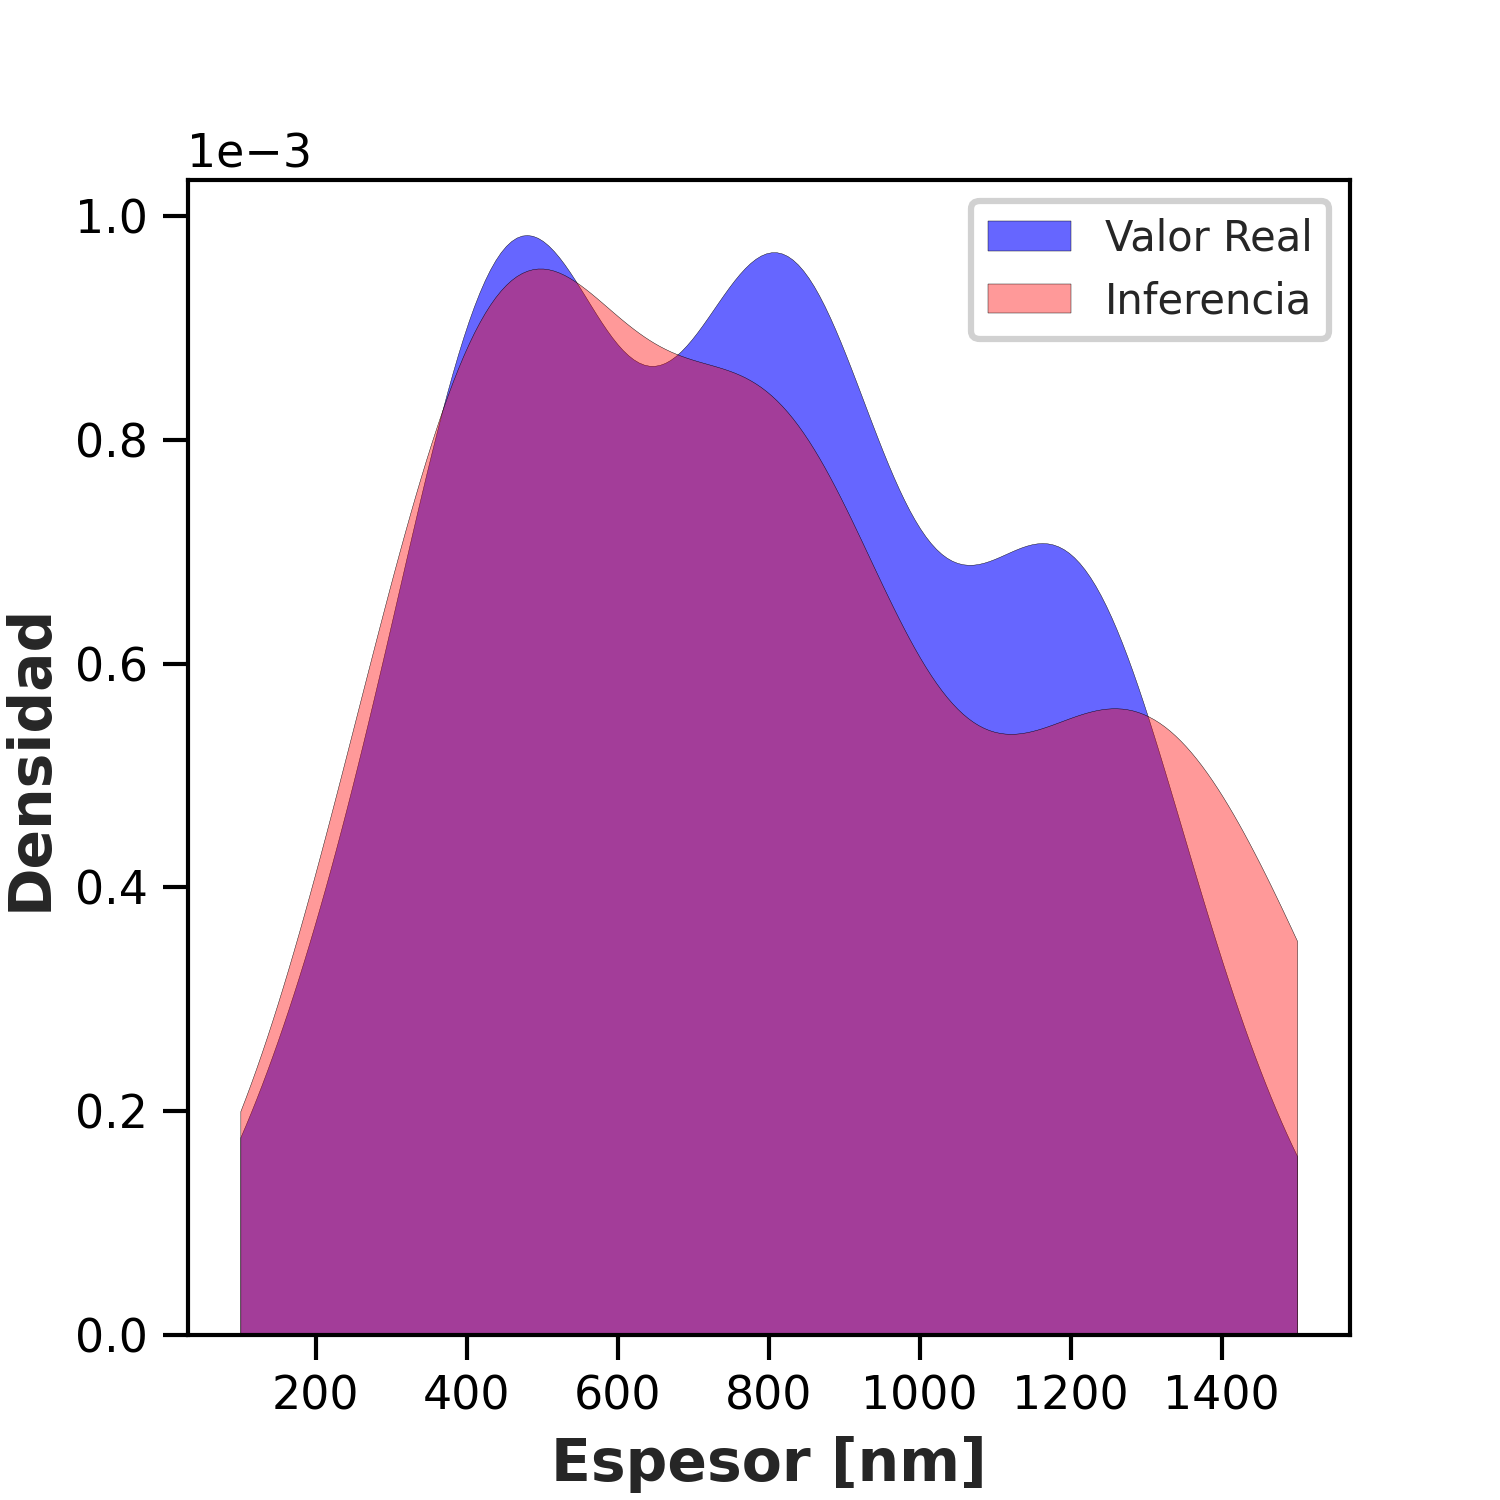
\includegraphics[width=0.48\textwidth]{145_two_dist.png}
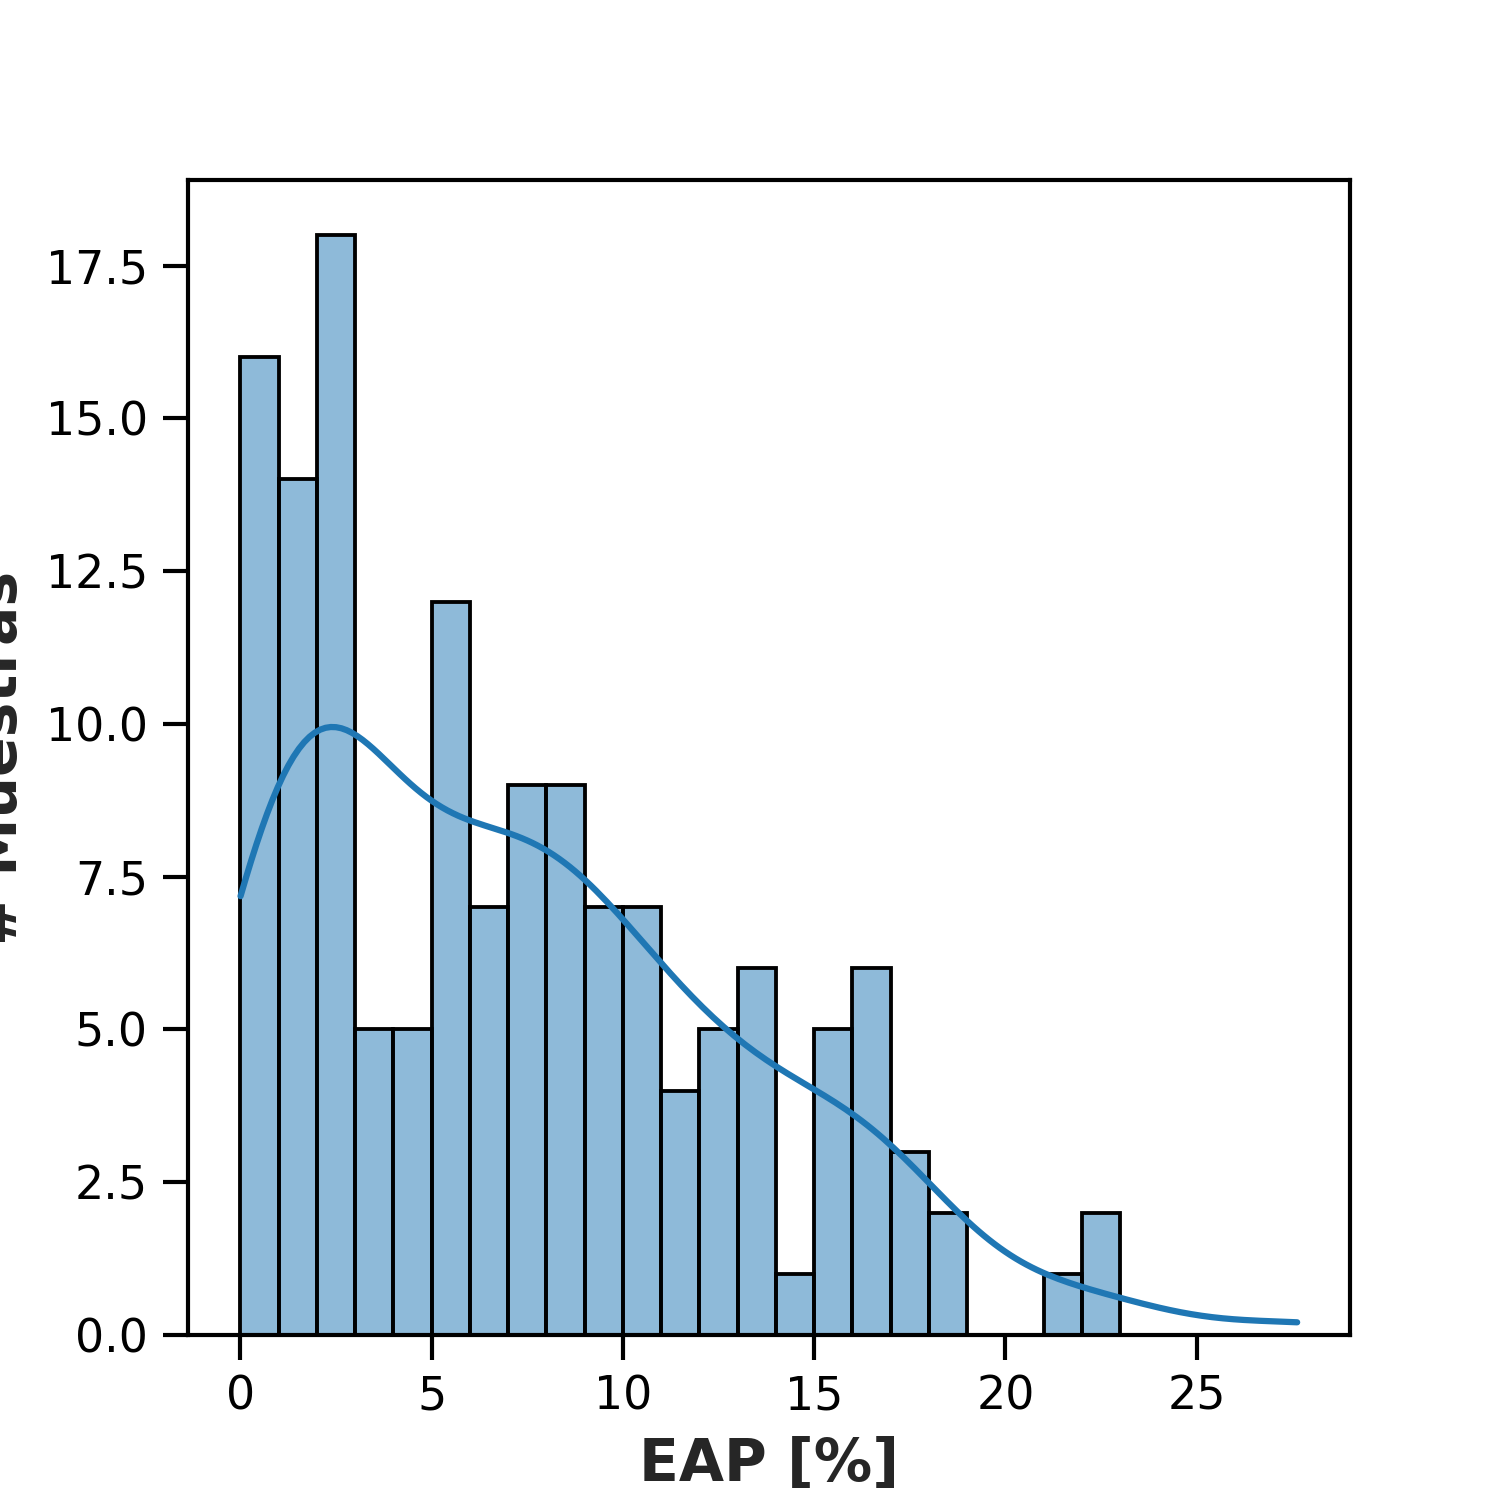
\includegraphics[width=0.48\textwidth]{145_hist.png}
\caption{Muestras experimentales 145: distribuciones superpuestas (izq.) e histograma (der.).}
\label{fig:145-2}
\end{figure}

\begin{figure}[htbp]
\centering
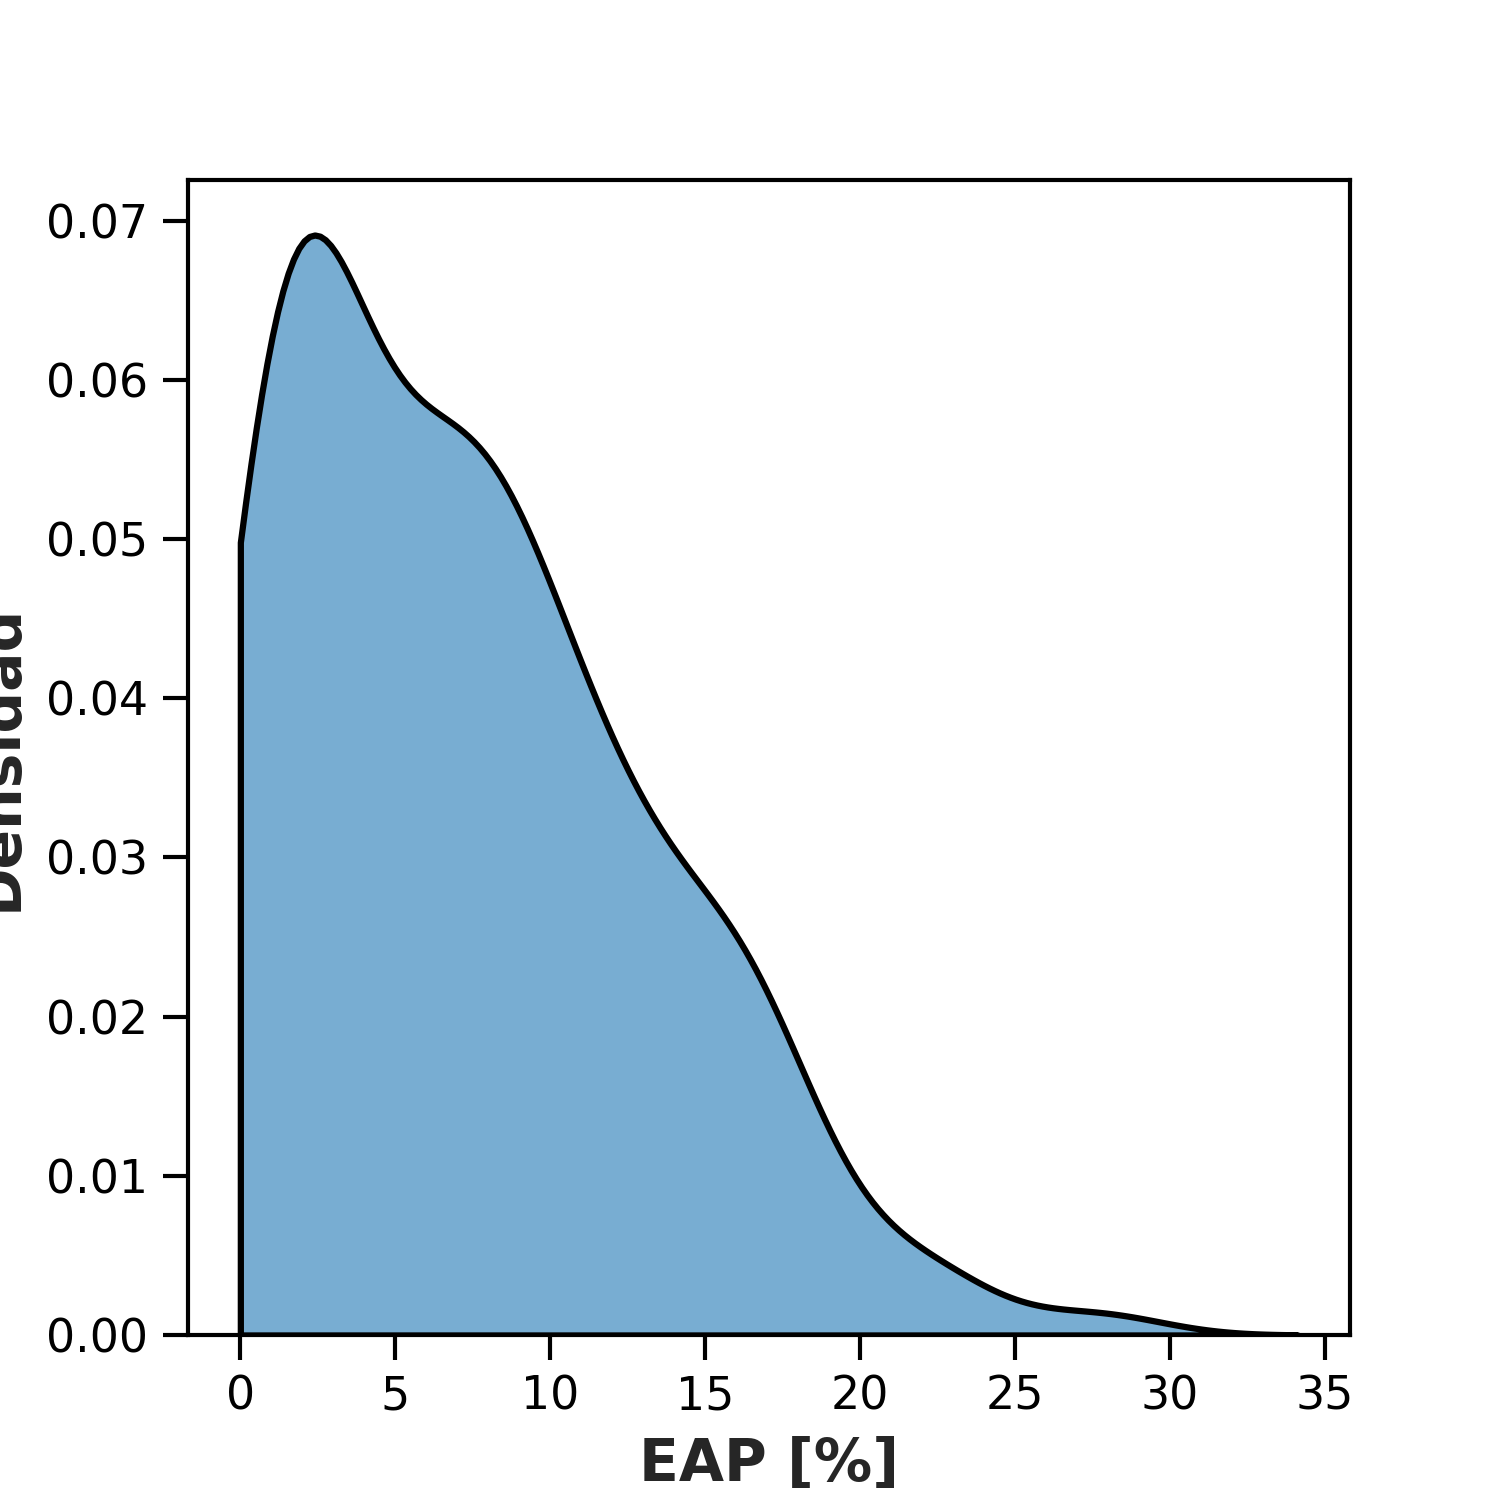
\includegraphics[width=0.48\textwidth]{145_dist_epa.png}
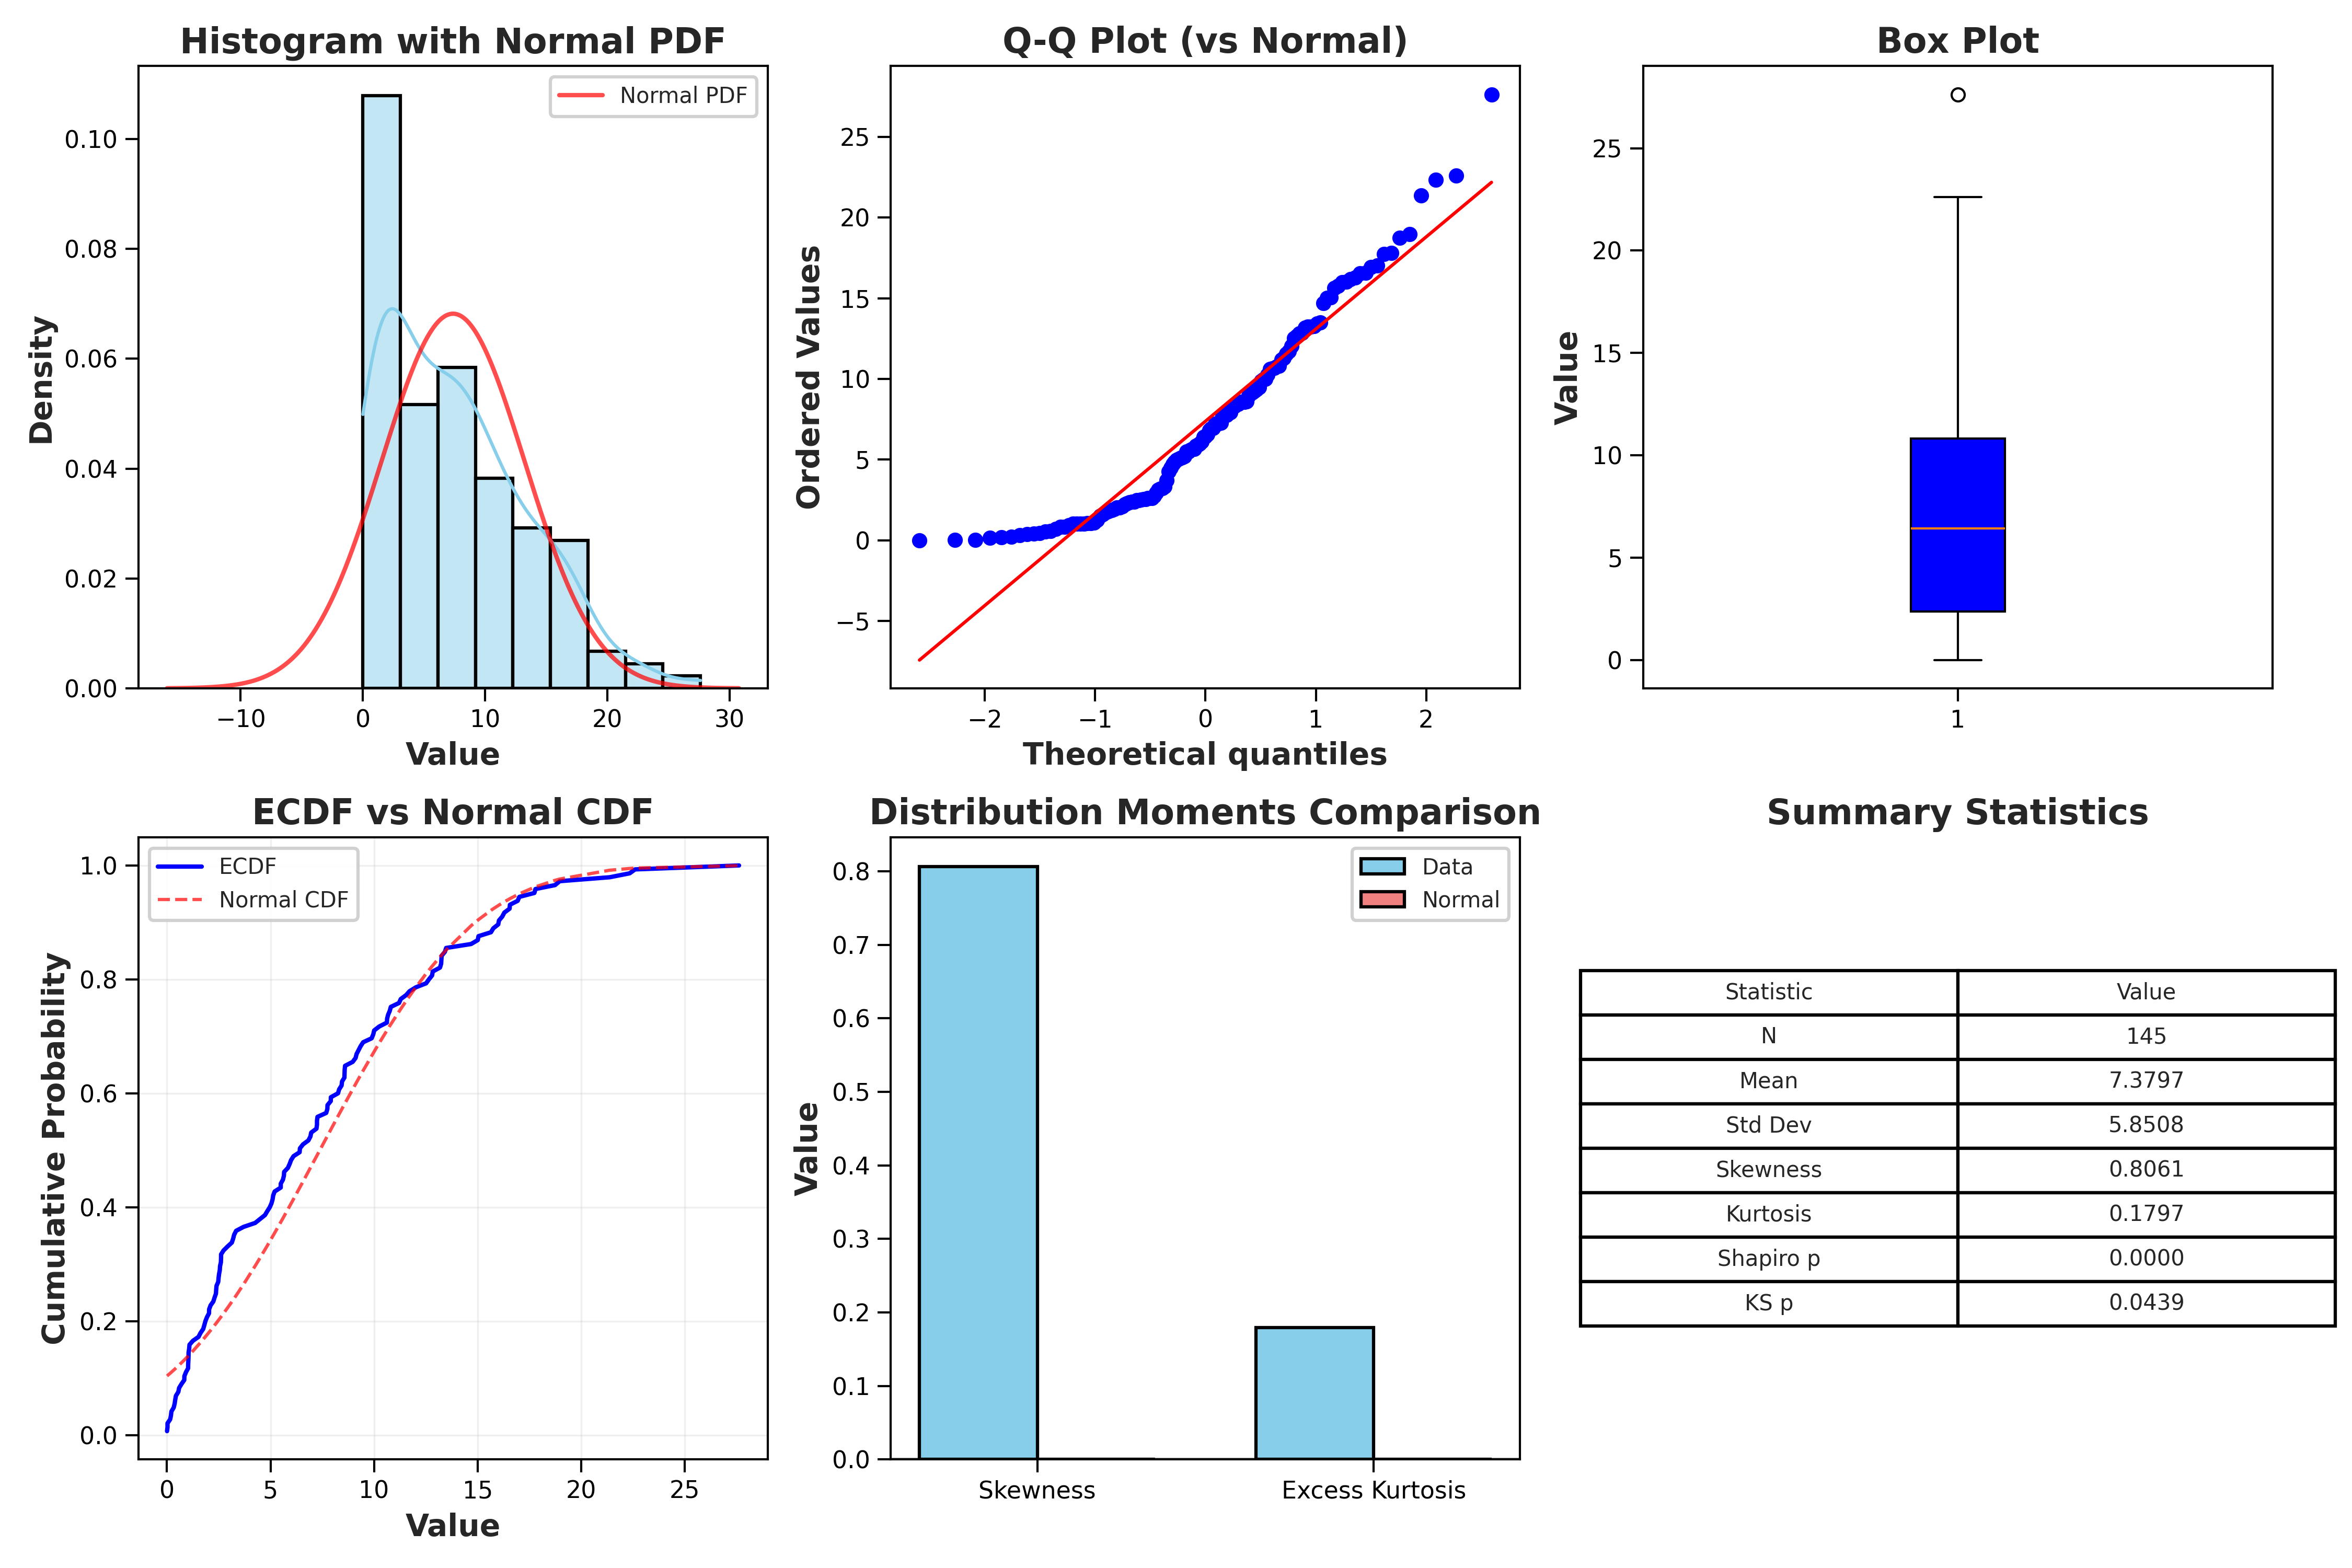
\includegraphics[width=0.48\textwidth]{145_dist_analysis_ape.png}
\caption{Muestras experimentales 145: distribución APE (izq.) y análisis diagnóstico APE (der.).}
\label{fig:145-3}
\end{figure}

\begin{figure}[htbp]
\centering
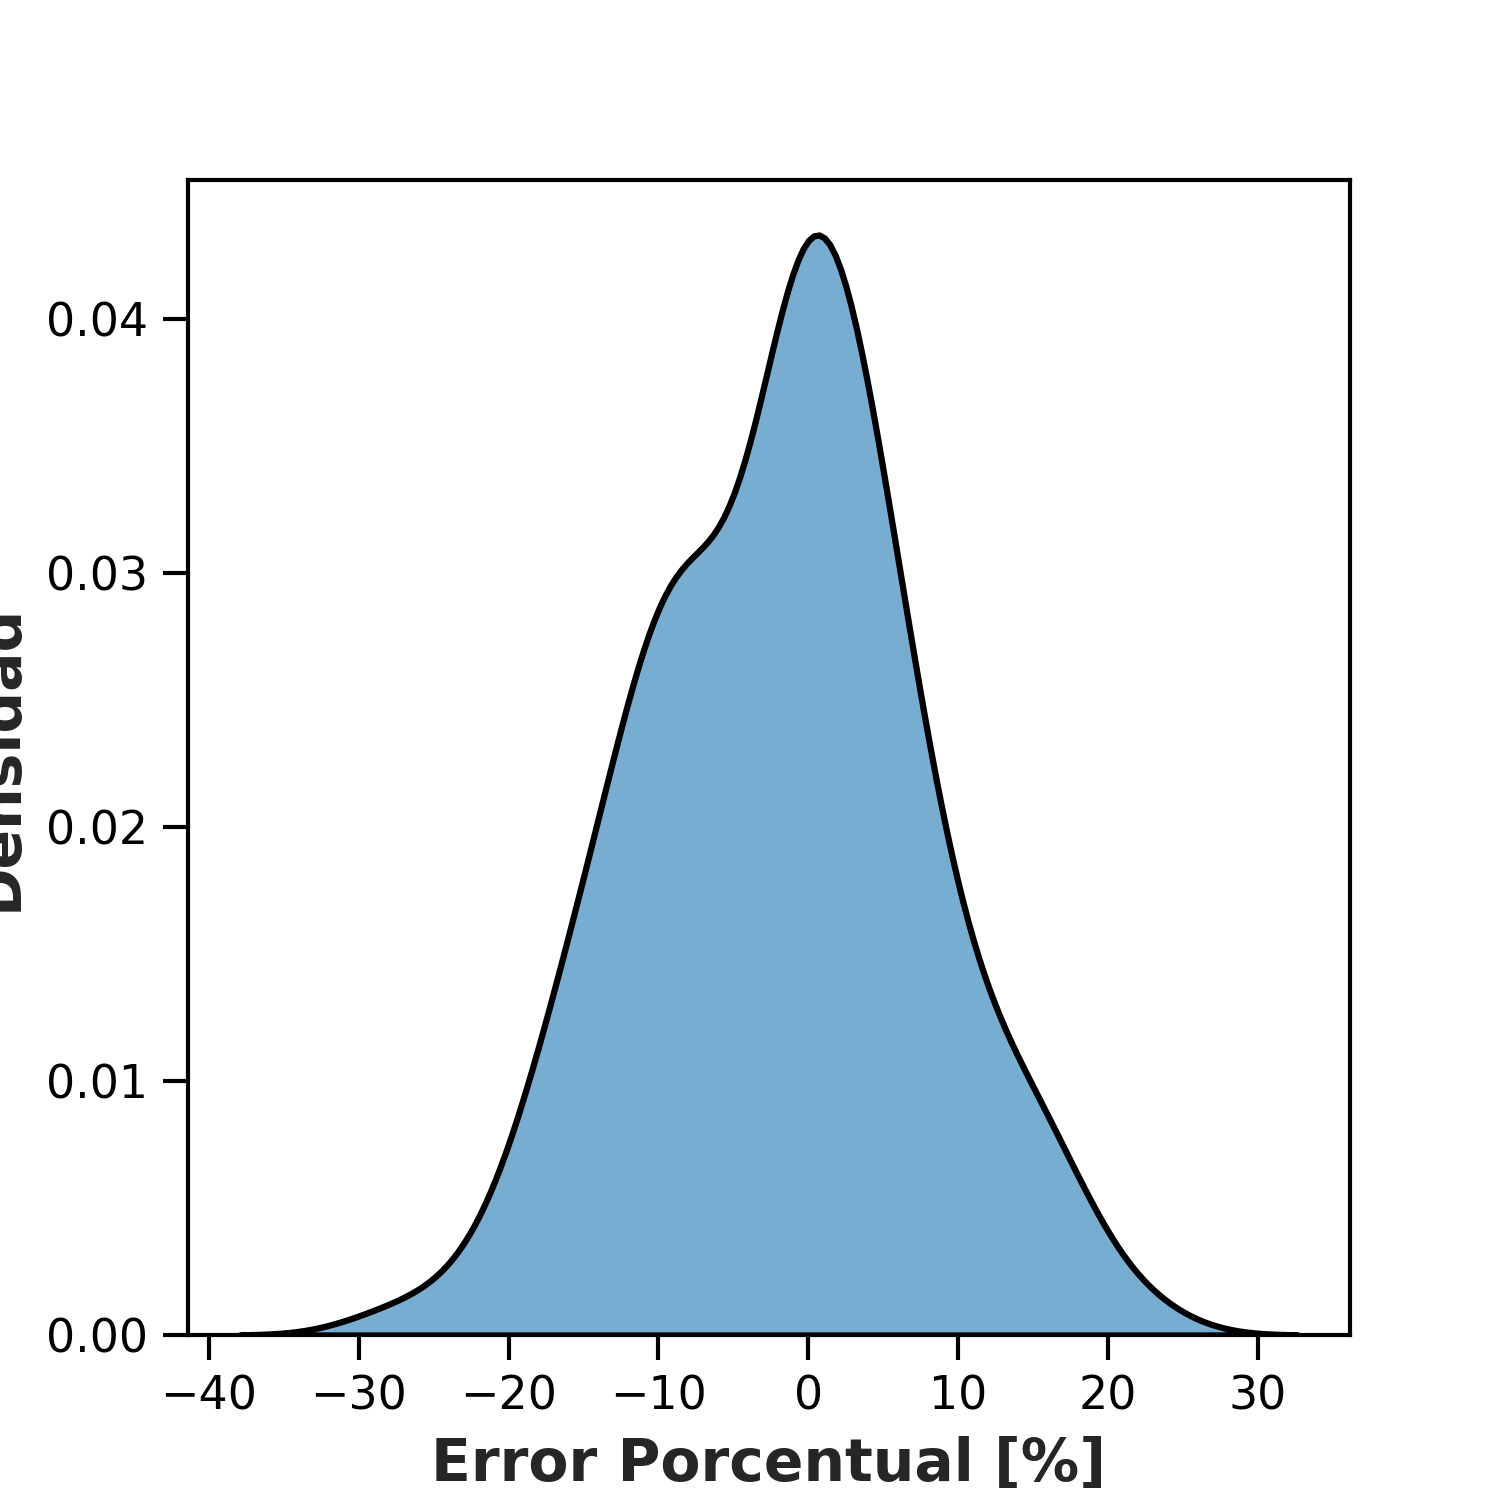
\includegraphics[width=0.48\textwidth]{145_dist_pe.png}
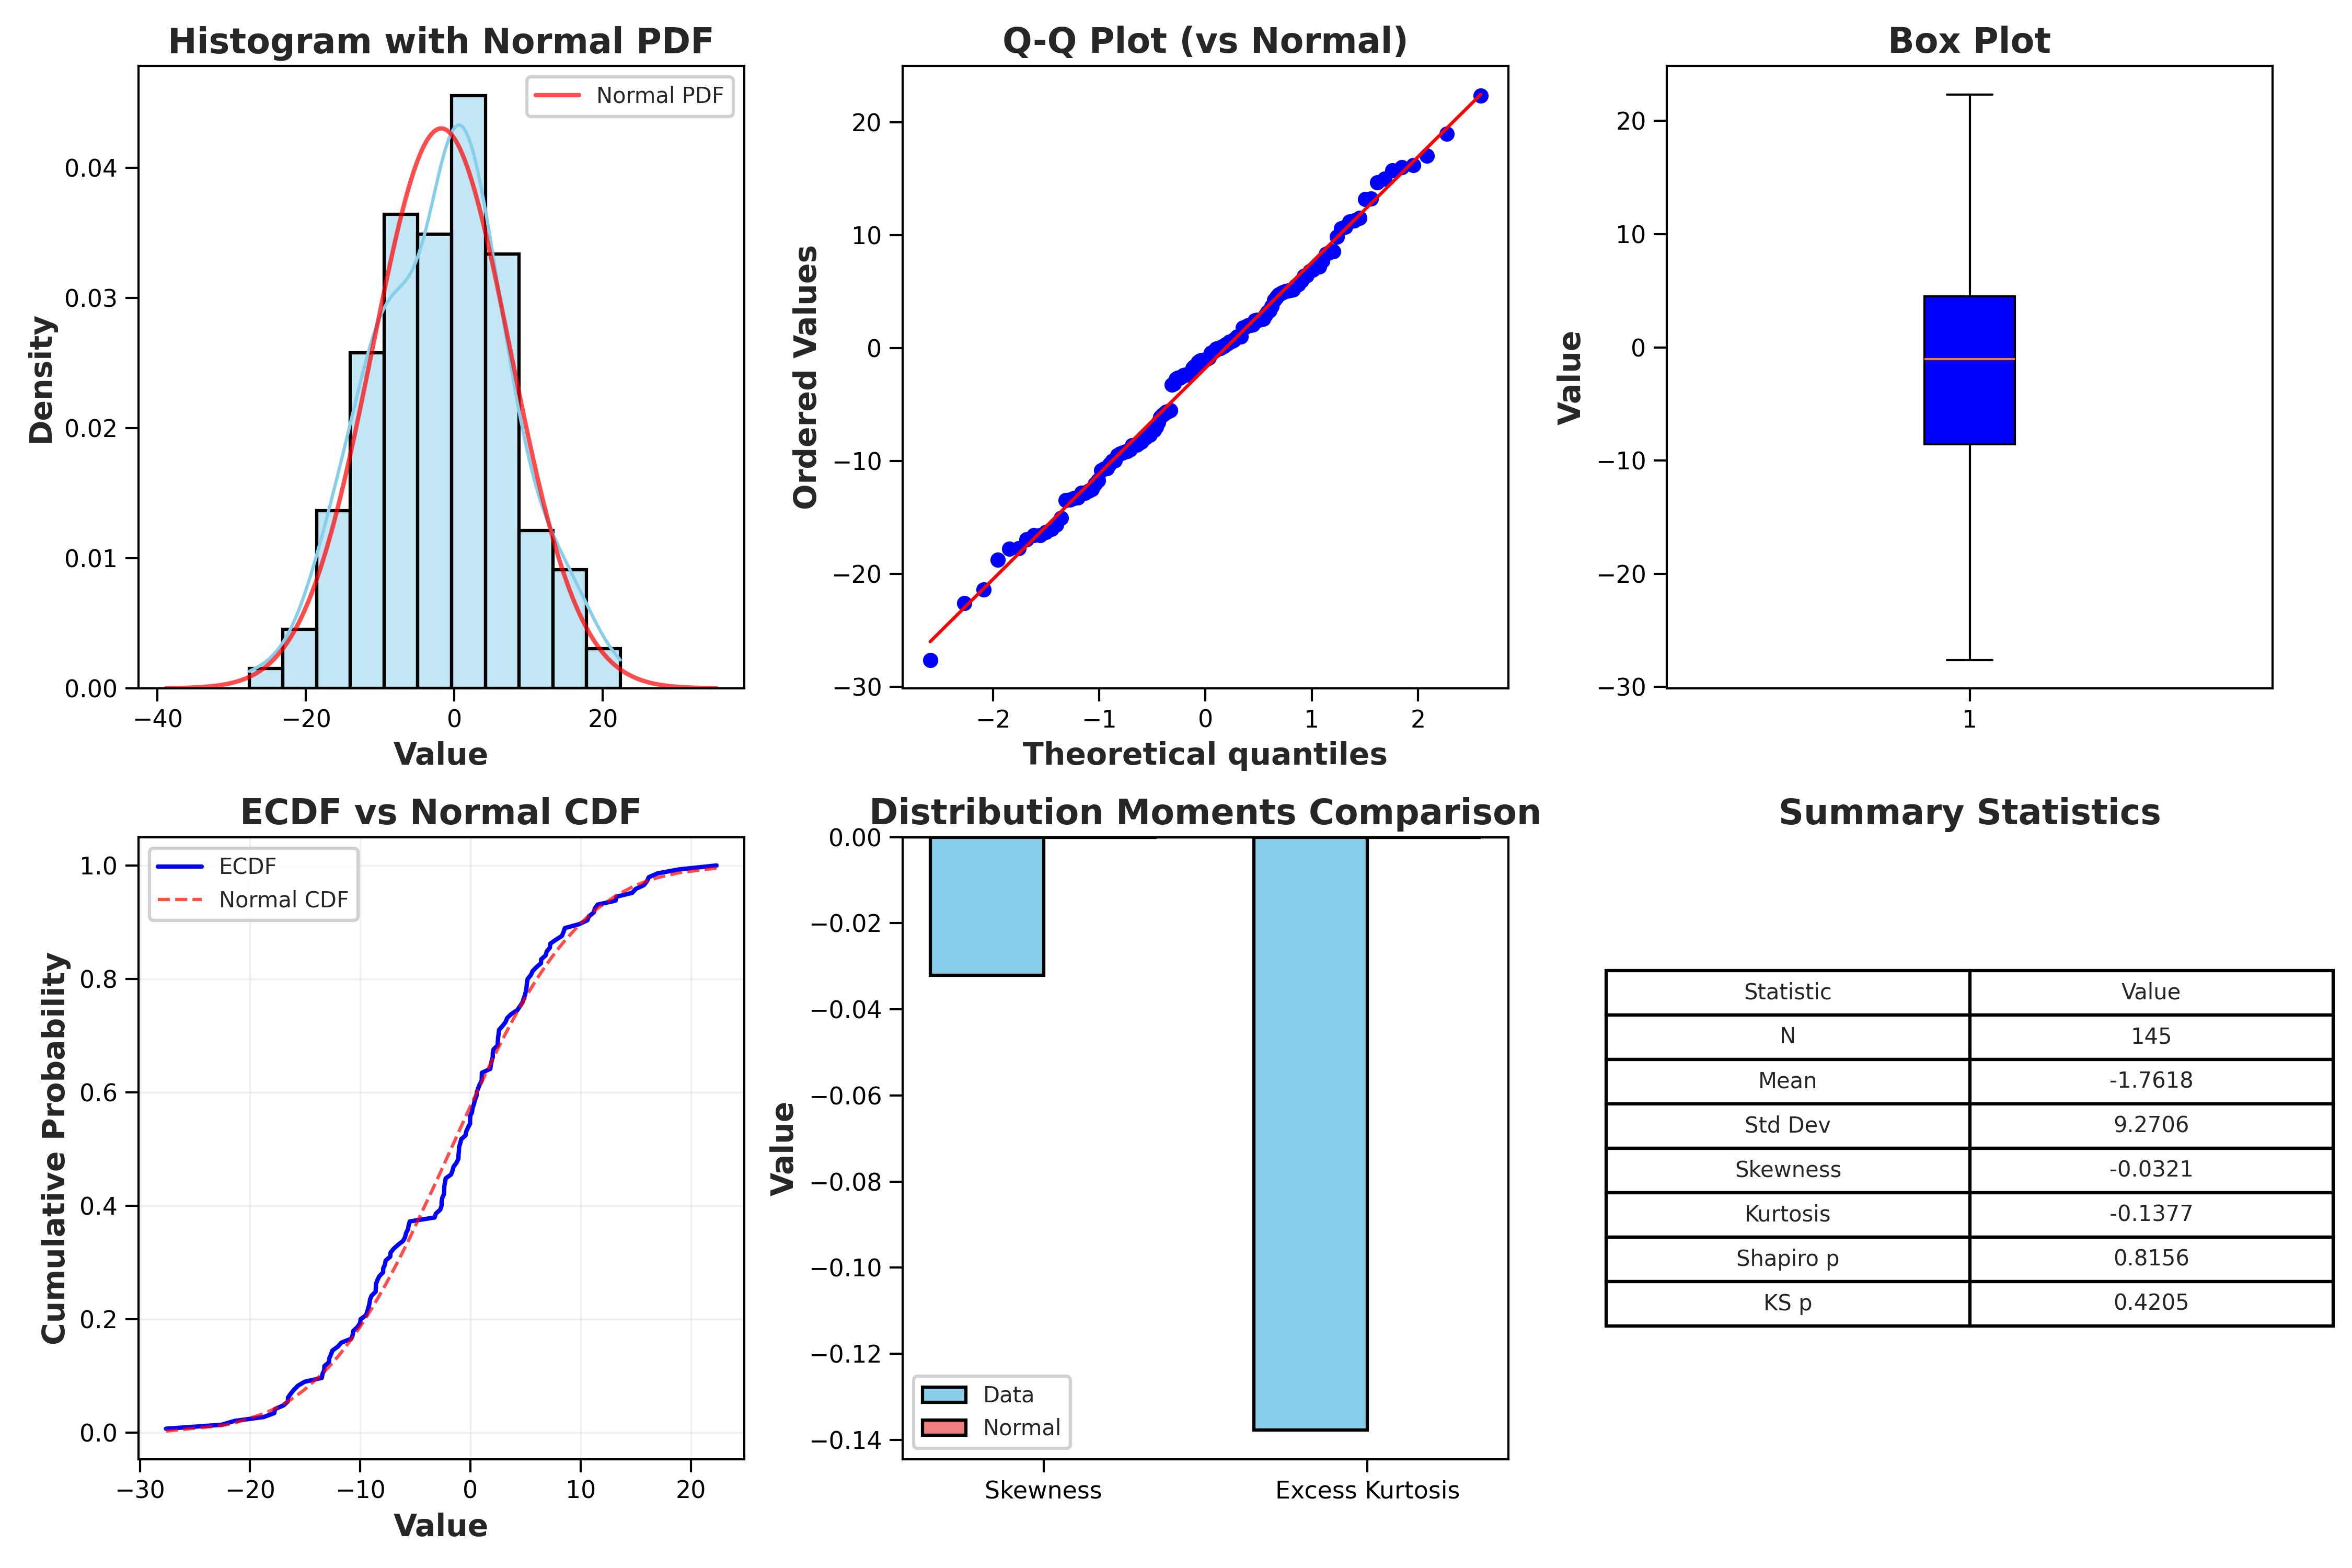
\includegraphics[width=0.48\textwidth]{145_dist_analysis_pe.png}
\caption{Muestras experimentales 145: distribución PE — ¡normalmente distribuida! (izq.) y análisis diagnóstico PE (der.).}
\label{fig:145-4}
\end{figure}

%%%%%%%%%%%%%%%%%%%%%%%%%%%%%%%%%%%%%%%%%%%%%%%%%%%%%%%%%%%%%%
\subsection{Comparación Entre Divisiones}
%%%%%%%%%%%%%%%%%%%%%%%%%%%%%%%%%%%%%%%%%%%%%%%%%%%%%%%%%%%%%%

\begin{table}[htbp]
\centering
\caption{Comparación completa de métricas entre las cuatro divisiones.}
\label{tab:cross-split}
\begin{tabular}{lcccccc}
\hline
División & $N$ & MAE (nm) & RMSE (nm) & MAPE (\%) & $R^2$ & APE Media (\%) & APE Mediana (\%) \\
\hline
Train      & 960,000 & 2.91  & 3.84  & 0.61 & 0.9999 & 0.6120 & 0.3273 \\
Validación & 120,000 & 2.91  & 3.85  & 0.61 & 0.9999 & 0.6095 & 0.3275 \\
Test       & 120,000 & 2.93  & 3.89  & 0.62 & 0.9999 & 0.6153 & 0.3280 \\
145 Exp.   & 145     & 58.77 & 83.84 & 7.38 & 0.9385 & 7.3797 & 6.4231 \\
\hline
\end{tabular}
\end{table}

\begin{table}[htbp]
\centering
\caption{Comparación de la forma de las distribuciones de error.}
\label{tab:dist-shape}
\begin{tabular}{lccccc}
\hline
División & APE Asimetría & APE Curtosis & PE Asimetría & PE Curtosis & PE ¿Normal? \\
\hline
Train      & +6.25 (der.) & 105.3 (leptocúrtica) & $-3.64$ (izq.) & 61.0 (leptocúrtica) & No \\
Validación & +6.52 (der.) & 124.7 (leptocúrtica) & $-4.13$ (izq.) & 70.9 (leptocúrtica) & No \\
Test       & +7.24 (der.) & 167.3 (leptocúrtica) & $-4.27$ (izq.) & 95.4 (leptocúrtica) & No \\
145 Exp.   & +0.81 (der.) & 0.18 (mesocúrtica)  & $-0.03$ (sim.)  & $-0.14$ (mesocúrtica) & \textbf{¡Sí!} ($p = 0.816$) \\
\hline
\end{tabular}
\end{table}

\textbf{Observaciones clave:}
\begin{itemize}
\item Las divisiones simuladas (Train/Val/Test) son \textbf{virtualmente indistinguibles} en todas las métricas, lo que proporciona fuerte evidencia de una generalización robusta y ausencia de sobreajuste.
\item El conjunto Experimental 145 muestra un MAPE aproximadamente \textbf{12$\times$ mayor}, lo cual es consistente con los desafíos adicionales de los espectros del mundo real: ruido, incertidumbre en la medición y desajuste del modelo entre simulación y experimento.
\item El $R^2$ de \textbf{0.9385} en datos experimentales sigue siendo alto, lo que demuestra que el modelo captura variación significativa de espesor incluso fuera de su distribución de entrenamiento.
\end{itemize}

\subsection{Análisis de Distribuciones: Resumen}

\textbf{Para todas las divisiones simuladas,} las distribuciones APE comparten una forma característica:
\begin{itemize}
\item Fuertemente sesgadas a la derecha (asimetría 6.2--7.2).
\item Extremadamente leptocúrticas (curtosis en exceso 105--167).
\item La mediana del APE es aproximadamente la mitad de la media ($\approx 0.33\%$ vs $\approx 0.61\%$), reflejando la cola derecha pesada.
\item Aproximadamente el 8.5\% de las muestras caen más allá del umbral de valores atípicos basado en IQR.
\item Rechazan la normalidad de manera decisiva en todas las pruebas ($p \approx 0$).
\end{itemize}

\textbf{Las distribuciones PE en las divisiones simuladas} reflejan este patrón en la cola izquierda (asimetría negativa $-3.6$ a $-4.3$, curtosis en exceso 60--95), lo que indica que los errores grandes tienden a ser sobre-predicciones.

\textbf{En contraste, el conjunto Experimental 145 exhibe:}
\begin{itemize}
\item PE aproximadamente \textbf{normal} (Shapiro-Wilk $p = 0.816$) — las cuatro pruebas de normalidad no logran rechazar la hipótesis nula.
\item Ligera asimetría positiva en APE.
\item Comportamiento mesocúrtico tanto en PE como en APE (curtosis en exceso cercana a cero).
\item Esta transición de \textbf{altamente leptocúrtico (simulado)} a \textbf{mesocúrtico (experimental)} puede reflejar el tamaño de muestra limitado ($N = 145$) o una estructura de error fundamentalmente diferente en datos reales.
\end{itemize}

\subsection{Conclusiones Finales del Capítulo}
\begin{itemize}
\item El modelo U-NET alcanza \textbf{MAPE = 0.61\%, RMSE = 3.85~nm, $R^2 = 0.9999$} en datos simulados, estableciendo un rendimiento de referencia excepcional.
\item En muestras experimentales reales, el modelo logra \textbf{MAPE = 7.38\%, $R^2 = 0.9385$}, demostrando una capacidad de generalización significativa a datos fuera de distribución.
\item El error PE en los datos experimentales presenta una \textbf{distribución normal} (hecho único entre todas las divisiones), lo que sugiere que los errores en datos reales se comportan como ruido Gaussiano aditivo.
\item Las métricas casi idénticas entre train/val/test confirman una excelente generalización y ausencia de sobreajuste.
\item El pipeline de extremo a extremo (datos experimentales $\rightarrow$ ajuste DE $\rightarrow$ simulación GMM $\rightarrow$ entrenamiento U-NET $\rightarrow$ inferencia) entrega exitosamente un \textbf{sistema práctico de predicción de espesor de películas delgadas}.
\end{itemize}

\subsection{Reproducibilidad}
\begin{itemize}
\item Modelo: UNET pre-entrenado guardado como archivo \texttt{.keras}.
\item Datos: Espectros simulados (HDF5) + espectros experimentales (PKL + NPY).
\item Entrenamiento: 100 épocas, Adam ($lr = 1 \times 10^{-3}$), sin programación de tasa de aprendizaje.
\item Pipeline de inferencia: \texttt{Predictions.py} $\rightarrow$ \texttt{training\_plots.py} $\rightarrow$ \texttt{1\_figures\_MSE.py}.
\item Directorio de salida: \texttt{MSE\_images/}.
\end{itemize}

\newpage

%%%%%%%%%%%%%%%%%%%%%%%%%%%%%%%%%%%%%%%%%%%%%%%%%%%%%%%%%%%%%%
%% CONCLUSIÓN
%%%%%%%%%%%%%%%%%%%%%%%%%%%%%%%%%%%%%%%%%%%%%%%%%%%%%%%%%%%%%%
\section{Conclusión}
\label{sec:conclusion}

El pipeline de extremo a extremo desarrollado en el proyecto AzONetV2 entrega exitosamente un sistema práctico de predicción de espesor de películas delgadas de AZO a partir de espectroscopía de transmitancia:

\begin{itemize}
\item \textbf{Procesamiento de datos experimentales:} Se consolidaron 145 muestras de AZO con espectros de transmitancia en el rango 190--1100~nm, corrigiendo valores de espesor y eliminando valores atípicos mediante inspección manual.

\item \textbf{Ajuste de modelo físico:} Se aplicó Evolución Diferencial (SciPy) para ajustar el modelo de transmitancia de Alonso (13 parámetros) a cada espectro experimental, minimizando el MSE. DE superó significativamente a Basin-Hopping y al algoritmo Direct, logrando un MSE cercano a cero de manera consistente.

\item \textbf{Simulación de datos:} Se ajustaron Modelos de Mezcla Gaussiana (GMM) a las distribuciones de parámetros por región de espesor (5 regiones), generando $\sim$1.2 millones de espectros sintéticos de transmitancia que preservan las propiedades estadísticas de los datos experimentales originales.

\item \textbf{Búsqueda de hiperparámetros:} La arquitectura U-NET superó a las DNN por un factor de 2$\times$ (MAPE 5.77\% vs 10.51\%), confirmando que las arquitecturas convolucionales son fundamentalmente más adecuadas para datos espectrales estructurados. La búsqueda en dos fases (descubrimiento de arquitectura + optimización de regularizadores) identificó $F=21$, nodos [470,340,330], $D=35\%$, y regularización L2 suave como configuración óptima.

\item \textbf{Entrenamiento de producción:} El modelo U-NET entrenado sobre el dataset sintético completo con pérdida MSE alcanzó MAPE = 0.61\% y RMSE = 3.85~nm en datos de validación. El cambio de MAE a MSE produjo una mejora relativa del 46\% en ambas métricas.

\item \textbf{Evaluación experimental:} En las 145 muestras experimentales externas, el modelo logró MAPE = 7.38\%, $R^2 = 0.9385$. Notablemente, la distribución del error porcentual en datos experimentales resultó ser normal (Shapiro-Wilk $p = 0.816$), con las cuatro pruebas de normalidad coincidiendo en no rechazar la hipótesis nula. Esto sugiere que los errores del modelo en datos reales se comportan como ruido Gaussiano aditivo no sesgado.
\end{itemize}

El proyecto demuestra que la combinación de modelado físico (Alonso IIM), optimización global (Evolución Diferencial), modelado generativo (GMM) y aprendizaje profundo (U-NET convolucional) constituye una estrategia efectiva para la caracterización no destructiva de películas delgadas semiconductoras.

\section*{Agradecimientos}
Este trabajo fue desarrollado como parte del proyecto AzONetV2.

% ============================================================
% BIBLIOGRAFÍA
% ============================================================
\begin{thebibliography}{99}

\bibitem{alonso} Alonso, et al.\ Modelo de transmitancia para películas delgadas semiconductoras. Método de Interferencia Inducida (IIM).

\bibitem{scipy} Virtanen, P., et al.\ (2020). SciPy 1.0: Fundamental Algorithms for Scientific Computing in Python. \textit{Nature Methods}, 17, 261--272.

\bibitem{keras} Chollet, F., et al.\ (2015). Keras. \url{https://keras.io}

\bibitem{tensorflow} Abadi, M., et al.\ (2016). TensorFlow: A system for large-scale machine learning. \textit{OSDI}, 265--283.

\bibitem{sklearn} Pedregosa, F., et al.\ (2011). Scikit-learn: Machine Learning in Python. \textit{JMLR}, 12, 2825--2830.

\bibitem{unet} Ronneberger, O., Fischer, P., \& Brox, T.\ (2015). U-Net: Convolutional Networks for Biomedical Image Segmentation. \textit{MICCAI}.

\bibitem{gmm} Bishop, C.\ M.\ (2006). Pattern Recognition and Machine Learning. Springer.

\bibitem{de} Storn, R., \& Price, K.\ (1997). Differential Evolution -- A Simple and Efficient Heuristic for Global Optimization. \textit{Journal of Global Optimization}, 11, 341--359.

\end{thebibliography}

\end{document}
